%\documentclass[a4paper,12pt,twoside]{book}
\documentclass[listof=nochaptergap,12pt,times,authoryear]{report}
\usepackage{mathptmx}%This package supersedes times and mathptm
\usepackage[a4paper,right=2.54cm,left=2.54cm,top=2.54cm,bottom=2.54cm]{geometry}
\usepackage{array}
\usepackage{listings}
\usepackage{pdflscape}
\usepackage{longtable}
\usepackage{enumitem}
\usepackage{newclude}
\usepackage[export]{adjustbox}
\newcolumntype{C}[1]{>{\centering\arraybackslash}p{#1}}
\newcolumntype{N}{@{}m{0pt}@{}}
\newcommand\fillin[1][3cm]{\makebox[#1]{\dotfill}}

%%Paquete para ocultar indices de tabla de contenidos
%% Numeración continua en figuras y tablas
\setcounter{equation}{0}
\usepackage{chngcntr}
\counterwithout{figure}{chapter}
\counterwithout{table}{chapter}
\counterwithout{equation}{chapter}
\renewcommand{\thefigure}{\arabic{figure}}
\renewcommand{\thetable}{\arabic{table}}
\renewcommand{\theequation}{\arabic{equation}}

% Parche para eliminar espacios por capítulos en lista de figuras y tablas
\usepackage{etoolbox}% http://ctan.org/pkg/etoolbox
\makeatletter
% \patchcmd{<cmd>}{<search>}{<replace>}{<succes>}{<failure>}
\patchcmd{\@chapter}{\addtocontents{lof}{\protect\addvspace{10\p@}}}{}{}{}% LoF
\patchcmd{\@chapter}{\addtocontents{lot}{\protect\addvspace{10\p@}}}{}{}{}% LoT
\makeatother


%%%%paquete para usar citas de diferentes formatos
%%%%%%%%%%%%%%%%%%%%%%%%%%%%%%%%%
%%add al indice
%\usepackage[nottoc,numbib]{tocbibind}
%\usepackage[authoryear,round]{natbib}
\usepackage[utf8]{inputenc}
\usepackage{csquotes}
\usepackage[spanish,es-lcroman]{babel}
\decimalpoint
%% Citas y bibliografía formato APA
\usepackage[backend=biber,style=apa,natbib=true]{biblatex}
%\DeclareLanguageMapping{australian}{australian-apa}
\DeclareLanguageMapping{spanish}{spanish-apa}
\addbibresource{biblio/references.bib}

%% Formato DOI
\DeclareFieldFormat{doi}{%
	doi\addcolon\space
	\ifhyperref
	{\lowercase{\href{https://doi.org/#1}{\nolinkurl{#1}}}}
	{\lowercase{\nolinkurl{#1}}}}

%% Formato de URL en referencias
\DeclareFieldFormat{url}{{Recuperado de}\space\url{#1}}

%% Convertir comando cita por textcite para que tenga formato APA
\let\cite\textcite

%% Para que texto de figuras y tablas tenga formato APA.
%% Caption se carga aqui con sus opciones (margin/font/labelfont) en una sola
%% invocacion, para evitar "Option clash" si se intentara recargar mas abajo.
\usepackage{multirow,booktabs,setspace}
\usepackage[margin=10pt,font=small,labelfont=bf]{caption}
\DeclareCaptionLabelSeparator*{spaced}{\\[2ex]}
\captionsetup[table]{labelfont=normalfont,textfont=it,format=plain,justification=justified,singlelinecheck=false,labelsep=newline,skip=2pt}
\captionsetup[figure]{labelsep=period,labelfont={it,bf},justification=justified,singlelinecheck=false,font=doublespacing}
\captionsetup[subfigure]{justification=centering}

%%%Editar formato y tamaño de capítulos y secciones
\usepackage{titlesec}
\titleformat{\chapter}
{\centering\normalfont\large\bfseries}{Capítulo \thechapter:}{1em}{}
\titlespacing*{\chapter}{0pt}{-4ex}{1ex}

\titleformat{\section}
{\normalfont\large\bfseries}{\thesection}{1em}{}
\titlespacing*{\section}{0pt}{0pt}{0pt}

\titleformat{\subsection}
{\normalfont\large\bfseries}{\thesubsection}{1em}{}
\titlespacing*{\subsection}{0pt}{0pt}{0pt}

%\usepackage{biblatex}
%paquete para hiperlinks entre citas e imagenes
%%%%%%%%%%%%%%%%%%%%%%%%%%%%%%%%%
\usepackage[colorlinks=true,
citecolor=black,
urlcolor=black,
bookmarks=true,
linkcolor=black,
pdftitle={Tesis-nombre-alumno},
pdfauthor={autor nombres}]{hyperref}

\usepackage{amssymb}
\usepackage{tikz}
\usetikzlibrary{shapes.geometric, shapes.symbols, arrows.meta, positioning, calc, fit, backgrounds, chains, decorations.pathreplacing}
\usepackage{graphicx} % for improved inclusion of graphics
%\usepackage{wrapfig} % to include figure with text wrapping around it
% caption ya cargado mas arriba con sus opciones; subcaption va aparte
\usepackage{subcaption}
\usepackage{eucal}
% color NO se carga aqui: lo carga xcolor (linea ~167) con [usenames,dvipsnames]
% combinado en sus opciones para evitar "Option clash for package color"
\usepackage[perpage]{footmisc}
%\usepackage[round, sort]{natbib}
\usepackage{ifthen}
\usepackage{multicol} % for pages with multiple text columns, e.g. References
\setlength{\columnsep}{20pt} % space between columns; default 10pt quite narrow
%% Para no mostrar índices de figuras ni tablas en el índice general
\usepackage[nottoc,notlot,notlof]{tocbibind}
%\usepackage{appendix}
\usepackage[titletoc,title]{appendix} 

%%%----Modificar encabezado y pie de pagina
%%%%%%%%%%%%%%%%%%%%%%%%%%%%%%%%%%%%%%%%%%%%%%%%%%%%%%%%%%%%%%%%%%%%%
\usepackage{fancyhdr} % for better header layout
\newcommand{\changefont}{%
	\fontsize{9pt}{1.5pt}\selectfont
}

\pagestyle{fancy}
%%Para borrar fancy por default (incluye numeracion)
\fancyhf{} % sets both header and footer to nothing
%%Para borrar linea de encabezado
\renewcommand{\headrulewidth}{0pt}
%%Encabezados solo con numero de pagina
\fancypagestyle{normal}{%
	\fancyhead{} % clear all header fields
	\fancyhead[R]{\thepage}}
%%Encabezados con titulo de tesis y numero de pagina
\fancypagestyle{special}{%
	\fancyhead[L]{\changefont Inteligencia Electoral con LLM: Minería de Sentimientos y Detección Dinámica de Temas Relevantes para analizar la Percepción Nacional en Ecosistemas Digitales}
	\fancyhead[R]{\thepage}}


%\fancyhf{} %% delete default configuration of page
%%\setlength\headheight{15pt}

%%%%%%%%%%%%%%%%%%%%%%%%%%%%%5
%%%% Configuracion de los parrafos
%\usepackage{setspace}
%\onehalfspacing
%\linespread{1.25} 
\setlength{\parindent}{0.5in} %%sangria
\setlength{\parskip}{3mm}  %%espacio entre parrafos
\linespread{1.3} %This equals 1.5 linespacing in Word
%%%% nuevo parrafo
%%%%%%%%%%%%%%%%%%%%%%%%%%%%%5
%%%% Centrar valores de una tabla
% array ya cargado al inicio del preambulo (linea 5)
%%CENTRADO HORIZONTAL
\newcolumntype{P}[1]{>{\centering\arraybackslash}p{#1}}
%%CENTRADO VERTICAL
\newcolumntype{M}[1]{>{\centering\arraybackslash}m{#1}}

%%%%%%%%%%%%%%%%%%%%%%%%%%%%%5
%%%%Paquete para alinear texto
\usepackage{ragged2e}
% multirow ya cargado mas arriba (linea 67)
\usepackage{makecell}
\usepackage{rotating}
\usepackage{siunitx} % To align the numbers later on
% xcolor carga internamente color con las mismas opciones (usenames, dvipsnames),
% evitando el "Option clash for package color"
\usepackage[usenames, dvipsnames, table, xcdraw]{xcolor}
\usepackage{colortbl}
\definecolor{Gray}{gray}{0.9}
\definecolor{orange}{rgb}{1,0.647,0}
\definecolor{turq3}{rgb}{0.54, 0.81, 0.94}
\definecolor{turq}{rgb}{0.63, 0.79, 0.95}
\definecolor{bluejean}{rgb}{0.03, 0.27, 0.49}

%% Estilo cypher para \lstinputlisting. Definido aqui (despues de cargar
%% listings, xcolor y los colores) para evitar el error
%% "File ended while scanning use of \lst@Delim@delim" que ocurre cuando
%% se pasan opciones complejas (con \color) en linea via archivos \input{}.
\lstdefinestyle{cypher}{%
    basicstyle=\ttfamily\footnotesize,%
    backgroundcolor=\color{gray!8},%
    frame=single,%
    framesep=4pt,%
    keywordstyle=\color{blue!70!black}\bfseries,%
    morekeywords={MATCH,MERGE,SET,ON,CREATE,WHERE,RETURN,WITH,UNWIND,AS,datetime},%
    commentstyle=\color{green!50!black}\itshape,%
    morecomment=[l]{//},%
    showstringspaces=false,%
    columns=fullflexible,%
    breaklines=true,%
    upquote=true%
}

%%%%%%%%%%%%%%%%%%%%%%%%%
\usepackage{xparse}
\usepackage{expl3}

%%%% Comando para figuras pendientes (placeholder vectorial).
%%%% Uso: \figpendiente{label}{caption corto LOF}{caption largo}
%%%% Renderiza un cuadro con texto "[FIGURA PENDIENTE]" + descripcion,
%%%% con su \caption y \label, para que las refs del texto resuelvan
%%%% mientras se prepara la imagen final. Reemplazar por
%%%% \includegraphics{...} cuando se tenga la imagen real.
\newcommand{\figpendiente}[3]{%
    \begin{figure}[!ht]
        \begin{center}
            \fbox{\parbox[c][3.2cm][c]{0.9\textwidth}{%
                \centering\bfseries\color{red!70!black}\large
                [FIGURA PENDIENTE]\\[6pt]
                \normalfont\normalsize\itshape\color{black} #2
            }}
            \caption[#2]{#3\\Fuente: Elaboración propia.}
            \label{#1}
        \end{center}
    \end{figure}%
}

%%%%funcion de reemplazar regex
\ExplSyntaxOn
\NewDocumentCommand{\replace}{mmm}
{
	\marian_replace:nnn {#1} {#2} {#3}
}

\tl_new:N \l_marian_input_text_tl
\tl_new:N \l_marian_search_tl
\tl_new:N \l_marian_replace_tl

\cs_new_protected:Npn \marian_replace:nnn #1 #2 #3
{
	\tl_set:Nn \l_marian_input_text_tl { #1 }
	\tl_set:Nn \l_marian_search_tl { #2 }
	\tl_set:Nn \l_marian_replace_tl { #3 }
	\regex_replace_all:nnN { \b\u{l_marian_search_tl}\b } { \u{l_marian_replace_tl} } \l_marian_input_text_tl
	\tl_use:N \l_marian_input_text_tl
}
\ExplSyntaxOff

%%%%%%%%%%%%%%%%%%%%%%%%%%%%%%%%%%%%%%
\usepackage{amsmath}
%\setcounter{equation}{0}
%\numberwithin{equation}{chapter} %%enumerar ecuaciones
%\renewcommand{\theequation}{Ecuación \arabic{equation}}   
\usepackage{mathtools, nccmath, cool}
%%%Configuraciones de biblatex

%%%hel
%%%%\citeauthor
\makeatletter

%%%%%%%%%%%%
\DeclareCiteCommand{\citeauthor}
{\boolfalse{citetracker}%
	\boolfalse{pagetracker}%
	\usebibmacro{prenote}}
{\ifciteindex
	{\indexnames{labelname}}
	{}%
	\printtext[bibhyperref]{\printnames{labelname}}}
{\multicitedelim}
{\usebibmacro{postnote}}


\DeclareCiteCommand{\citetitle}
{\boolfalse{citetracker}%
	\boolfalse{pagetracker}%
	\usebibmacro{prenote}}
{\ifciteindex
	{\indexfield{indextitle}}
	{}%
	\printtext[bibhyperref]{\printfield[citetitle]{labeltitle}}}
{\multicitedelim}
{\usebibmacro{postnote}}

\DeclareCiteCommand{\cite}
{\usebibmacro{prenote}}
{\usebibmacro{citeindex}%
	\printtext[bibhyperref]{\usebibmacro{cite}}}
{\multicitedelim}
{\usebibmacro{postnote}}

\DeclareCiteCommand*{\cite}
{\usebibmacro{prenote}}
{\usebibmacro{citeindex}%
	\printtext[bibhyperref]{\usebibmacro{citeyear}}}
{\multicitedelim}
{\usebibmacro{postnote}}

\DeclareCiteCommand{\parencite}[\mkbibparens]
{\usebibmacro{prenote}}
{\usebibmacro{citeindex}%
	\printtext[bibhyperref]{\usebibmacro{cite}}}
{\multicitedelim}
{\usebibmacro{postnote}}

\DeclareCiteCommand*{\parencite}[\mkbibparens]
{\usebibmacro{prenote}}
{\usebibmacro{citeindex}%
	\printtext[bibhyperref]{\usebibmacro{citeyear}}}
{\multicitedelim}
{\usebibmacro{postnote}}

\DeclareCiteCommand{\footcite}[\mkbibfootnote]
{\usebibmacro{prenote}}
{\usebibmacro{citeindex}%
	\printtext[bibhyperref]{ \usebibmacro{cite}}}
{\multicitedelim}
{\usebibmacro{postnote}}

\DeclareCiteCommand{\footcitetext}[\mkbibfootnotetext]
{\usebibmacro{prenote}}
{\usebibmacro{citeindex}%
	\printtext[bibhyperref]{\usebibmacro{cite}}}
{\multicitedelim}
{\usebibmacro{postnote}}

\DeclareCiteCommand{\textcite}
{\boolfalse{cbx:parens}}
{\usebibmacro{citeindex}%
	\printtext[bibhyperref]{\usebibmacro{textcite}}}
{\ifbool{cbx:parens}
	{\bibcloseparen\global\boolfalse{cbx:parens}}
	{}%
	\multicitedelim}
{\usebibmacro{textcite:postnote}}
\makeatother
\makeatletter
\let\abx@macro@citeOrig\abx@macro@cite
\renewbibmacro{cite}{%
	\bibhyperref{%
		\let\bibhyperref\relax\relax%
		\abx@macro@citeOrig%
	}%
}
\let\abx@macro@textciteOrig\abx@macro@textcite
\renewbibmacro{textcite}{%
	\bibhyperref{%
		\let\bibhyperref\relax\relax%
		\abx@macro@textciteOrig%
	}%
}%

\makeatother

%%%%%%%%%%%%%%%%%%%%%%%%%%%%%%%%%%%%%%%%%%%
% Agregando librerias para que aparezca texto debajo de las ecuaciones.
\usepackage[titles]{tocloft}

%% Para agregar palabra "CAPÍTULO" en 
\newlength\mynewlength
\let\oldcftchappresnum\cftchappresnum
\renewcommand*\cftchappresnum{Capítulo \oldcftchappresnum}
\renewcommand\cftchapaftersnum{:}
\settowidth\mynewlength{\cftchappresnum\cftchapaftersnum\quad}
\addtolength\cftchapnumwidth{\mynewlength}

\usepackage{xpatch}
% caption ya cargado al inicio del preambulo
\DeclareCaptionType{equcaption}[Ecuación][Índice de Ecuaciones]

\newenvironment{conditions}
{\par\vspace{\abovedisplayskip}\noindent\begin{tabular}{>{$}l<{$} @{${}={}$} l}}
	{\end{tabular}\par\vspace{\belowdisplayskip}}

% Para agregar linea de puntos en la tabla de contenidos
\renewcommand{\cftpartleader}{\cftdotfill{\cftdotsep}} % for parts
\renewcommand{\cftchapleader}{\cftdotfill{\cftdotsep}} % for chapters

% Para eliminar linea de puntos de la tabla de contenidos
%\renewcommand{\cftdot}{}

% Para alinear párrafo en indice de figuras y tablas
\cftsetindents{figure}{0em}{2.5em}
\renewcommand\cftfigpresnum{\figurename~}
\renewcommand{\cftfigaftersnum}{.} % Goes after figure number
\newlength\mylength
\settowidth\mylength{\cftfigpresnum}
\addtolength\cftfignumwidth{\mylength}
\cftsetindents{table}{0em}{2.5em}
\renewcommand\cfttabpresnum{Tabla }
\renewcommand{\cfttabaftersnum}{.} % Goes after figure number
\settowidth\mylength{\cfttabpresnum}
\addtolength\cfttabnumwidth{\mylength}

\DefineBibliographyExtras{spanish}{%
	\savecommand\sptext
	\renewcommand*{\sptext}{\textsuperscript}}

\UndefineBibliographyExtras{spanish}{%
	\restorecommand\sptext}

%%Formato APA (No funciona en biblatex)
\usepackage{apalike}
%\bibliographystyle{apalike}

\begin{document}
% Se añade esto para agregar la lista de ecuaciones en el indice del documento	

\newcommand{\listequationsname}{Índice de Ecuaciones}
\newlistof{myequations}{equ}{\listequationsname}
\newcommand{\myequations}[1]{%
	\addcontentsline{equ}{myequations}{Ecuación \protect\numberline{\theequation}#1}\par}
%\addcontentsline{toc}{section}{Índice de Ecuaciones}

%%Numeros de pagina en romano (minuscula)
%\pagenumbering{roman}
\renewcommand{\thepage}{\roman{page}}

% Beginning of hack...
%\let\oldthispagestyle=\thispagestyle % If we want to see a page number.
%\def\thispagestyle#1{} % If we want to see a page number.
%\let\oldsetcounter=\setcounter
%\def\setcounter#1#2{}
% End of hack...

\begin{titlepage}

	\begin{center}
		%%%cargar imagen
	    
\includegraphics[width=0.20\textwidth]{images/esanlogomin.png}
		\vspace*{2cm} \\
		UNIVERSIDAD ESAN \vspace*{1ex} \\
		FACULTAD DE INGENIERÍA \vspace*{1ex} \\
		INGENIERÍA DE TECNOLOGÍAS DE INFORMACIÓN Y SISTEMAS
		\vspace*{8ex} \\
		%\textbf
		{Inteligencia Electoral con LLM: Minería de Sentimientos y Detección Dinámica de Temas Relevantes para analizar la Percepción Nacional en Ecosistemas Digitales}
		\vspace*{8ex}\\	
		Tesis para optar el Título de Ingeniero de Tecnologías de Información y Sistemas que presenta: 
		\vspace*{8ex} \\	
		Axel Denis Cuadros Huachua \\
		Victor Manuel Ormeño Salazar \\
		Piero Luis Rojas Paucar \\
		Jeferson Joseph Sandoval Díaz \vspace*{2cm}\\

		Asesor: Marks Arturo Calderón Niquin		
		\vfill
		Lima, \today 
		
	\end{center}
\end{titlepage}
%%Permite mostrar encabezado y numeracion en primera pagina de capitulos - indices
\fancypagestyle{plain}{}
%%cambiar nombres de objetos para el indice y otros
\renewcommand{\listfigurename}{Índice de Figuras}
\renewcommand{\tablename}{Tabla}
\renewcommand{\listtablename}{Índice de Tablas}
%%Permite empezar conteo de paginas de forma personalizada
\addtocounter{page}{1}
\pagestyle{normal}
% % %\thispagestyle{plain}
% %\vspace{0.5cm}
% \leftline{Esta tesis denominada:}
% \begin{center}
% 	%\vspace*{10cm}
% 	{PREDICCIÓN DEL ESTADO DE FINANCIAMIENTO DE PROYECTOS DE TECNOLOGÍA EN SITIO WEB DE CROWDFUNDING KICKSTARTER MEDIANTE MODELO DE APRENDIZAJE PROFUNDO MULTIMODAL}
% \end{center}

% \leftline{ha sido aprobada.}
% \vspace{3cm}

% %\dotfill
% \rightline{\fillin[9cm]}
% \rightline{Eber Joseph Ballón Álvarez (Jurado Presidente)}
% \vspace{3cm}

% %\dotfill
% \rightline{\fillin[9cm]}
% \rightline{Wilfredo Mamani Ticona (Jurado)}
% \vspace{3cm}

% %\dotfill
% \rightline{\fillin[9cm]}
% \rightline{Pedro Nelson Shiguihara Juárez (Jurado)}
% \vspace{3cm}

% \centerline{Universidad ESAN}
% \centerline{2021}
%\thispagestyle{plain}
\begin{center}
	\vspace*{10cm}
	{INTELIGENCIA ELECTORAL CON LLM: MINERÍA DE SENTIMIENTOS Y DETECCIÓN DINÁMICA DE TEMAS RELEVANTES PARA ANALIZAR LA PERCEPCIÓN NACIONAL EN ECOSISTEMAS DIGITALES}
\end{center}

%\thispagestyle{plain}
\begin{center}
	%\vspace*{1.5cm}
	{\large \bfseries  Agradecimiento y Dedicatoria}
\end{center}
\vspace{0.5cm}

Thx
\newline



% outline
\tableofcontents            % print the table of contents

%: ----------------------- contents ------------------------

\setcounter{secnumdepth}{3} % organisational level that receives a numbers
\setcounter{tocdepth}{3}    % print table of contents for level 3

% levels are: 0 - chapter, 1 - section, 2 - subsection, 3 - subsection


%: ----------------------- list of figures/tables ------------------------
\clearpage
\listoffigures
\clearpage
\listoftables  % print list of tables
\clearpage
\phantomsection
%\listofequcaptions % print list of equations
\listofmyequations
\clearpage
%% Numeros de pagina en arabic (si se desea continuar la numeración)
%\renewcommand{\thepage}{\arabic{page}}
%% Para reiniciar la numeración
\pagenumbering{arabic}
%%Encabezado con titulo de tesis y numeracion
\pagestyle{special}
%La línea de abajo es para quitar encabezado
%\thispagestyle{plain}

\chapter*{Resumen}
\markboth{Resumen}{Resumen}
\addcontentsline{toc}{chapter}{Resumen}

En los procesos electorales contemporáneos, los ecosistemas digitales generan grandes volúmenes de información provenientes de múltiples fuentes como prensa digital, plataformas audiovisuales y redes sociales. Sin embargo, los enfoques tradicionales de análisis de opinión pública presentan limitaciones al tratar estas fuentes de manera homogénea, ignorando sus diferencias estructurales y la relación entre discurso mediático y percepción ciudadana. En este contexto, la presente investigación propone un sistema de Inteligencia Electoral basado en Modelos de Lenguaje de Gran Escala (LLMs), orientado a la minería de sentimientos y la detección dinámica de temas relevantes para analizar la percepción nacional en entornos digitales.

La propuesta integra un enfoque multi-fuente que combina datos provenientes de periódicos digitales, YouTube y Twitter/X, permitiendo capturar tres dimensiones del proceso electoral: el discurso mediático, el discurso audiovisual y la reacción ciudadana. Sobre esta base, se implementa una arquitectura tipo Medallion extendida, en la cual los datos son procesados mediante técnicas de filtrado eficiente, análisis semántico con LLMs y clustering inductivo de temas. Posteriormente, la información es estructurada en un grafo de conocimiento temporal, donde se modelan relaciones como cobertura mediática, co-ocurrencia de temas, sesgo editorial y la brecha entre medios y ciudadanía.

Adicionalmente, se incorpora un sistema GraphRAG que permite realizar consultas en lenguaje natural sobre el grafo, integrando información estructurada y textual para generar respuestas fundamentadas. Este enfoque posibilita no solo identificar tendencias de sentimiento y temas dominantes, sino también analizar dinámicas complejas como la evolución temporal de la opinión pública, el encuadre mediático y las diferencias entre percepción institucional y ciudadana.

Los resultados esperados evidencian que la integración de LLMs, grafos de conocimiento y análisis multi-fuente permite superar las limitaciones de los enfoques tradicionales, proporcionando una visión más rica y contextualizada del comportamiento electoral. De esta manera, la investigación contribuye con un modelo innovador de inteligencia electoral, así como con un prototipo analítico capaz de apoyar la toma de decisiones estratégicas y el estudio de la opinión pública en contextos latinoamericanos.

\textbf{Palabras claves: } inteligencia electoral, modelos de lenguaje de gran escala (LLMs), minería de sentimientos, detección de temas, grafos de conocimiento, GraphRAG, análisis multi-fuente, opinión pública.

\clearpage

\chapter*{Abstract}
\markboth{Abstract}{Abstract}

In contemporary electoral processes, digital ecosystems generate massive volumes of information from multiple sources such as digital news media, audiovisual platforms, and social networks. However, traditional approaches to public opinion analysis present limitations by treating these sources homogeneously, ignoring their structural differences and the relationship between media discourse and citizen perception. In this context, this research proposes an Electoral Intelligence system based on Large Language Models (LLMs), focused on sentiment mining and dynamic topic detection to analyze national perception in digital environments.

The proposed approach integrates a multi-source framework combining data from digital newspapers, YouTube, and Twitter/X, capturing three key dimensions of the electoral process: media discourse, audiovisual discourse, and citizen reaction. Based on this, an extended Medallion architecture is implemented, where data is processed through efficient filtering techniques, semantic analysis using LLMs, and inductive topic clustering. The processed information is then structured into a temporal knowledge graph, modeling relationships such as media coverage, topic co-occurrence, editorial bias, and the gap between media and citizens.

Additionally, a GraphRAG-based system is incorporated, enabling natural language queries over the knowledge graph by combining structured and unstructured information to generate grounded responses. This approach allows not only the identification of sentiment trends and dominant topics, but also the analysis of complex dynamics such as temporal evolution of public opinion, media framing, and divergences between institutional and citizen perception.

Expected results indicate that the integration of LLMs, knowledge graphs, and multi-source analysis overcomes the limitations of traditional approaches, providing a richer and more contextualized understanding of electoral behavior. Thus, this research contributes an innovative electoral intelligence model, along with an analytical prototype capable of supporting strategic decision-making and advancing the study of public opinion in Latin American contexts.

\textbf{Keywords: } electoral intelligence, large language models (LLMs), sentiment mining, topic detection, knowledge graphs, GraphRAG, multi-source analysis, public opinion.
%La línea de abajo es para quitar encabezado
%\thispagestyle{plain}

\chapter*{Introducción}
\markboth{Introducción}{Introducción}
\addcontentsline{toc}{chapter}{Introducción}

En los últimos años, especialmente con la masificación de las redes sociales y plataformas digitales, los procesos electorales han dejado de analizarse únicamente a través de encuestas tradicionales para incorporar nuevas fuentes de información que reflejan la opinión pública en tiempo real. Periódicos digitales, plataformas audiovisuales como YouTube y redes sociales como Twitter/X generan grandes volúmenes de datos que capturan tanto el discurso mediático como la percepción ciudadana. Entre estos entornos digitales, han surgido nuevas dinámicas de comunicación política, así como nuevas oportunidades de investigación orientadas a comprender cómo se construye y evoluciona la opinión pública durante campañas electorales.

A diferencia de investigaciones anteriores, donde la mayoría de enfoques se enfoca en el análisis de una única fuente de datos o en el uso de modelos tradicionales de procesamiento de lenguaje natural, la motivación central de este estudio es plantear un enfoque integral de Inteligencia Electoral que permita el análisis conjunto de diversas fuentes heterogéneas. En este contexto, se pretende superar las limitaciones derivadas del uso de una sola plataforma —como los sesgos de representación o la carencia de contexto— mediante la integración de información proveniente de prensa digital, contenido audiovisual y redes sociales. El principal aporte radica en el diseño de un sistema basado en Modelos de Lenguaje de Gran Escala (LLMs), el cual no solo realiza minería de sentimientos, sino que también identifica dinámicamente temas relevantes y modela las relaciones entre actores, fuentes y tópicos a través de un grafo de conocimiento temporal.

Asimismo, la propuesta incorpora un enfoque innovador al considerar explícitamente la diferencia entre el discurso mediático y la reacción ciudadana, permitiendo analizar la brecha entre ambos como un indicador clave en el comportamiento electoral. Esta aproximación se complementa con el uso de técnicas avanzadas como clustering inductivo de temas y sistemas GraphRAG, los cuales permiten realizar consultas en lenguaje natural sobre la información estructurada y no estructurada, facilitando la generación de insights complejos y contextualizados.

En el Capítulo I, se expone la problemática de la investigación dentro del contexto de los procesos electorales y los entornos digitales. De igual manera, se plantean los problemas, objetivos, hipótesis, justificación y delimitación del estudio.

En el Capítulo II, se detallan los antecedentes principales relacionados con el análisis de sentimiento político, el uso de modelos de lenguaje, el análisis multi-fuente y los grafos de conocimiento en contextos electorales. Posteriormente, se presenta el marco teórico que sustenta la investigación, abordando conceptos de procesamiento de lenguaje natural, inteligencia artificial, análisis de opinión y comunicación política digital.

En el Capítulo III, se describe el diseño metodológico de la investigación, incluyendo el tipo, enfoque, población y muestra. Asimismo, se detalla la arquitectura del sistema propuesto, basada en un enfoque tipo Medallion, así como el pipeline de procesamiento de datos, desde la ingesta hasta la construcción del grafo de conocimiento. Finalmente, se expone la metodología de evaluación y el cronograma de actividades.

En el Capítulo IV, se desarrolla la implementación de la solución propuesta, incluyendo la integración de fuentes de datos, el uso de LLMs para el análisis semántico, la detección de temas mediante clustering y la construcción del grafo de conocimiento, así como el sistema de consulta basado en GraphRAG.

En el Capítulo V, se presentan y analizan los resultados obtenidos, evaluando el desempeño del sistema en términos de detección de sentimientos, coherencia temática y capacidad de generación de insights. Asimismo, se discuten los hallazgos relacionados con la dinámica de la opinión pública y la brecha entre medios y ciudadanía.

En el Capítulo VI, se presentan las conclusiones de la investigación y se proponen recomendaciones orientadas a futuras líneas de trabajo, incluyendo posibles mejoras en la arquitectura del sistema y la extensión del análisis a otros contextos electorales.

La investigación concluye con las referencias bibliográficas utilizadas y los anexos que complementan la información presentada a lo largo del documento.
%\newcommand\chap[1]{%
%	\chapter*{#1}%
%	\addcontentsline{toc}{chapter}{#1}}


%%Num. de capitulos en romano y el resto en arabic
\renewcommand{\thechapter}{\Roman{chapter}}
\renewcommand{\thesection}{\arabic{chapter}.\arabic{section}}
\renewcommand{\thesubsection}{\arabic{chapter}.\arabic{section}.\arabic{subsection}}

% Este es el comando que funciona para las ecuaciones
\renewcommand{\theequcaption}{\arabic{equcaption}}

%%Para insertar los capítulos de forma seguida
\chapter{Planteamiento del Problema}

\section{Descripción de la Realidad Problemática}

En la última década, el crecimiento acelerado de los ecosistemas digitales ha transformado profundamente la manera en que se construye y percibe la opinión pública, especialmente en contextos electorales. Plataformas digitales como redes sociales, medios de comunicación en línea y servicios de contenido audiovisual han pasado a ser canales predominantes de información política, permitiendo a los ciudadanos expresar opiniones, consumir contenido y participar activamente en el debate público en tiempo real.

De acuerdo con \textcite{cr_digital2025}, más del 64\% de la población mundial utiliza redes sociales, lo que evidencia la masificación de estos entornos como espacios clave para la interacción social y política. Como se observa en la Figura \ref{fig:social_media_global}, este crecimiento ha consolidado a las plataformas digitales como un componente fundamental en la formación de la opinión pública contemporánea.

\begin{figure}[h]
	\begin{center}
		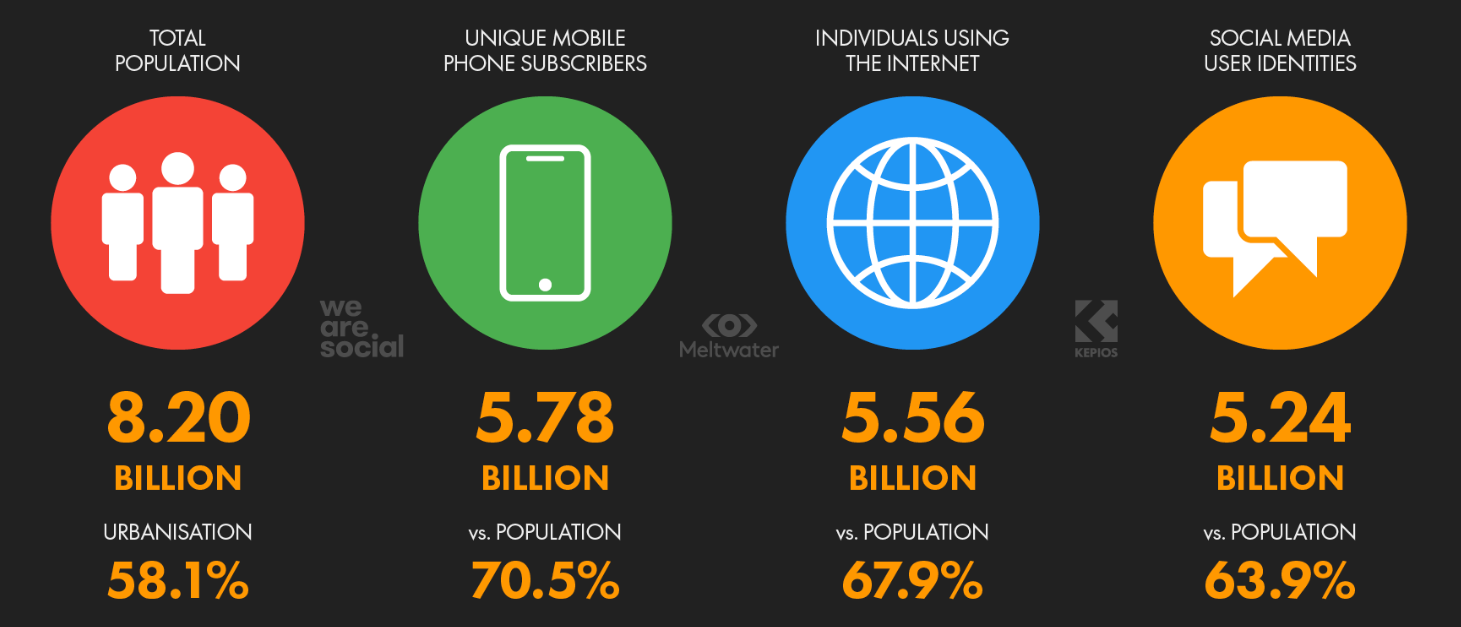
\includegraphics[width=0.7\textwidth]{images/social_media_global.png}
		\caption[Uso global de redes sociales]{Uso global de redes sociales (2025).\\
		Fuente: \textcite{cr_digital2025}.}
		\label{fig:social_media_global}
	\end{center}
\end{figure}

En América Latina, esta tendencia es aún más pronunciada. Según el \textcite{cr_reuters2024}, aproximadamente el 70\% de los usuarios accede a noticias a través de redes sociales, lo que ha incrementado significativamente la influencia de estas plataformas en la formación de percepciones políticas. Tal como se aprecia en la Figura \ref{fig:news_social}, el consumo de información política en entornos digitales ha superado a los medios tradicionales en diversos segmentos de la población.

\begin{figure}[h]
	\begin{center}
		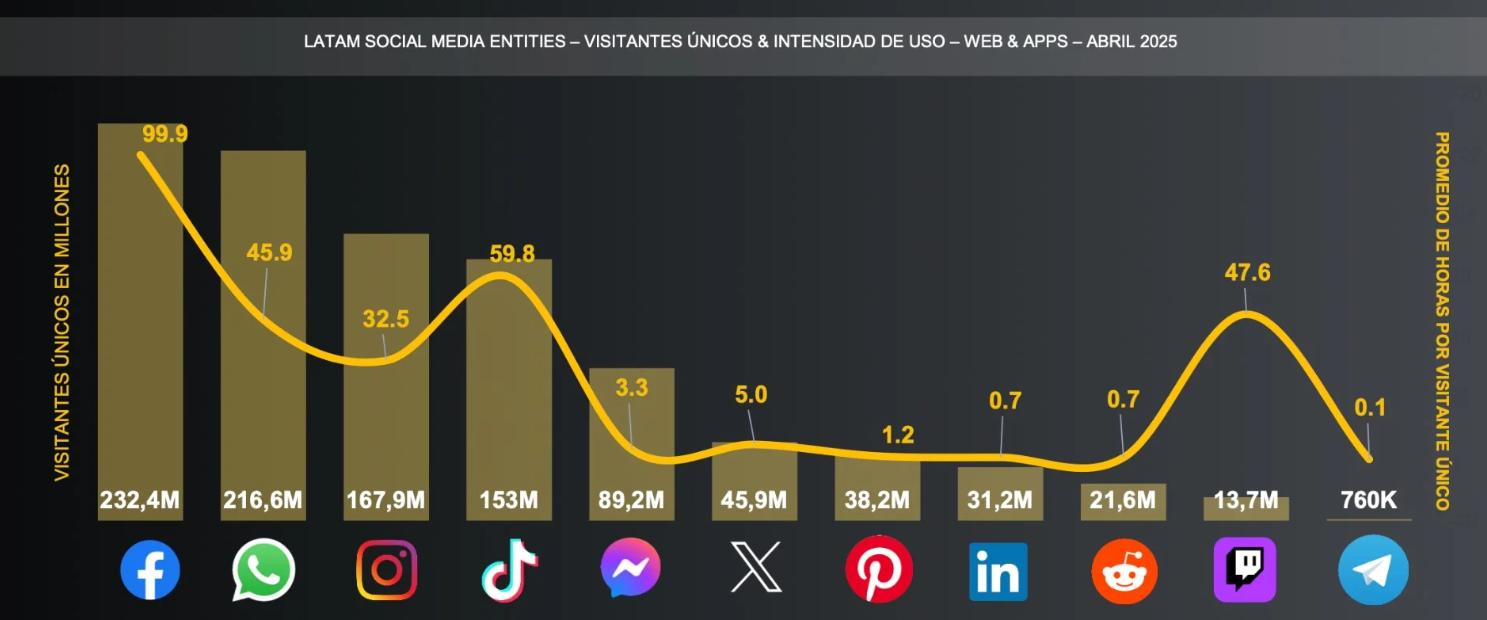
\includegraphics[width=0.7\textwidth]{images/news_social_media.png}
		\caption[Consumo de noticias en redes sociales]{Consumo de noticias a través de redes sociales en América Latina.\\
		Fuente: \textcite{cr_reuters2024}.}
		\label{fig:news_social}
	\end{center}
\end{figure}

En el caso específico del Perú, el acceso a Internet ha alcanzado aproximadamente el 82\% de la población, lo que equivale a más de 28 millones de usuarios conectados, según el Instituto Nacional de Estadística e Informática \parencite{cr_inei2024}. Como se muestra en la Figura \ref{fig:internet_peru}, este alto nivel de penetración digital refuerza la relevancia de analizar la percepción pública en entornos digitales dentro del contexto nacional.

\begin{figure}[h]
	\begin{center}
		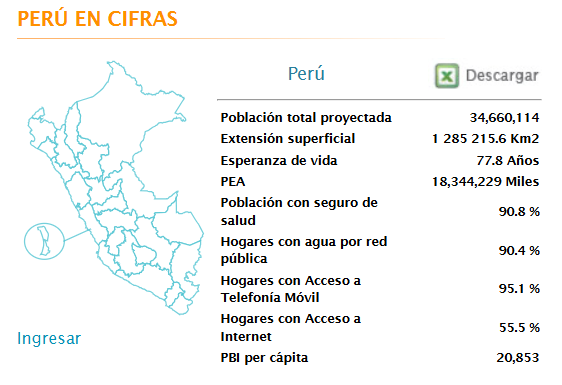
\includegraphics[width=0.65\textwidth]{images/internet_peru.png}
		\caption[Usuarios de internet en Perú]{Acceso a Internet en Perú (2024).\\
		Fuente: \textcite{cr_inei2024}.}
		\label{fig:internet_peru}
	\end{center}
\end{figure}

Sin embargo, este crecimiento también ha generado nuevos desafíos. La sobrecarga informativa, la desinformación y la polarización dificultan la comprensión precisa de la percepción ciudadana en contextos electorales. Tal como señala \textcite{cr_castells2015comunicacion}, la comunicación digital ha dado lugar a una dinámica en la que los ciudadanos no solo consumen información, sino que también la reinterpretan y amplifican, generando múltiples capas de significado.

En este contexto, los métodos tradicionales de análisis de opinión pública, como encuestas o estudios cualitativos, presentan limitaciones importantes debido a su costo, baja frecuencia y limitada capacidad de capturar dinámicas en tiempo real. Por otro lado, los enfoques computacionales existentes suelen centrarse en una sola fuente de datos, como redes sociales, ignorando la diversidad de actores y formatos presentes en el ecosistema digital.

Asimismo, existe una brecha significativa entre el discurso mediático y la percepción ciudadana. Mientras los medios de comunicación establecen agendas informativas, los ciudadanos reaccionan de manera independiente en redes sociales, generando diferencias que no son adecuadamente modeladas por los enfoques actuales. Esta problemática resulta crítica durante procesos electorales, donde la identificación de tendencias, temas relevantes y cambios en la percepción pública es fundamental.

Por otro lado, el avance de los Modelos de Lenguaje de Gran Escala (LLMs) ha abierto nuevas oportunidades para el análisis semántico profundo de grandes volúmenes de datos. Según \textcite{cr_bommasani2021foundation}, estos modelos permiten capturar relaciones complejas en el lenguaje natural, superando las limitaciones de técnicas tradicionales de procesamiento de lenguaje natural.

En consecuencia, se identifica la necesidad de desarrollar un enfoque integral que permita analizar la percepción nacional en contextos electorales mediante la integración de múltiples fuentes de información, el uso de modelos avanzados de lenguaje y la representación estructurada de relaciones mediante grafos de conocimiento.

\section{Formulación del Problema}

\subsection{Problema General}
PG: \newcommand{\ProblemaGeneral}{
¿Es posible analizar la percepción nacional en contextos electorales mediante un sistema de Inteligencia Electoral basado en modelos de lenguaje de gran escala (LLMs), minería de sentimientos y detección dinámica de temas en ecosistemas digitales multi-fuente?
}
\ProblemaGeneral

\subsection{Problemas Específicos}

\newcommand{\Pbone}{¿Qué enfoques existen en la literatura para el análisis de opinión pública mediante inteligencia artificial?}
\newcommand{\Pbtwo}{¿Cómo integrar múltiples fuentes de datos (noticias digitales, Twitter/X, YouTube y TikTok) para representar la percepción pública?}
\newcommand{\Pbthree}{¿Cuál es el impacto del uso de LLMs en el análisis de sentimientos y detección de temas?}
\newcommand{\Pbfour}{¿Cómo modelar las relaciones entre discurso mediático y percepción ciudadana mediante grafos de conocimiento?}

\begin{itemize}
	\item PE1: {\Pbone}
	\item PE2: {\Pbtwo}
	\item PE3: {\Pbthree}
	\item PE4: {\Pbfour}
\end{itemize}


\section{Objetivos de la Investigación}

\subsection{Objetivo General}
OG: \newcommand{\ObjetivoGeneral}{
Analizar la percepción nacional en contextos electorales mediante un sistema basado en LLMs, minería de sentimientos y detección de temas en ecosistemas digitales.
}
\ObjetivoGeneral
\subsection{Objetivos Específicos}

\newcommand{\Objone}{Analizar enfoques existentes en la literatura.}
\newcommand{\Objtwo}{Diseñar una arquitectura multi-fuente.}
\newcommand{\Objthree}{Evaluar el desempeño de LLMs en análisis de sentimientos y detección de temas.}
\newcommand{\Objfour}{Implementar un sistema basado en grafos de conocimiento y GraphRAG.}


\begin{itemize}
	\item OE1: {\Objone}
	\item OE2: {\Objtwo}
	\item OE3: {\Objthree}
	\item OE4: {\Objfour}
\end{itemize}

\section{Hipótesis}

\subsection{Hipótesis General}
HG: \newcommand{\HipotesisGeneral}{
El uso de modelos de lenguaje de gran escala (LLMs) permite analizar con mayor precisión la percepción nacional en entornos digitales multi-fuente durante contextos electorales.
}
\HipotesisGeneral
\subsection{Hipótesis Específicas}

\newcommand{\Hone}{La integración de múltiples fuentes de datos mejora la representatividad de la percepción pública.}
\newcommand{\Htwo}{Los modelos LLMs mejoran la precisión del análisis de sentimientos y detección de temas.}
\newcommand{\Hthree}{El uso de grafos de conocimiento permite modelar relaciones complejas entre actores y discursos.}
\newcommand{\Hfour}{El enfoque GraphRAG mejora la generación de insights en el análisis electoral.}

\begin{itemize}
	\item HE1: \Hone
	\item HE2: \Htwo
	\item HE3: \Hthree
	\item HE4: \Hfour
\end{itemize}


\section{Justificación de la Investigación}

\subsection{Teórica}

La presente investigación se justifica desde una perspectiva teórica debido a la necesidad de integrar enfoques contemporáneos en el análisis de la percepción pública dentro de ecosistemas digitales. Tradicionalmente, los estudios en análisis de opinión y comportamiento electoral se han apoyado en técnicas estadísticas clásicas y métodos de análisis de contenido manual o semiautomático. Sin embargo, el crecimiento exponencial de datos generados en redes sociales y plataformas digitales ha evidenciado limitaciones en dichos enfoques, especialmente en términos de escalabilidad, contextualización semántica y capacidad de adaptación en tiempo real.

En este contexto, el desarrollo de modelos de lenguaje de gran escala (LLMs) ha transformado significativamente el campo del Procesamiento de Lenguaje Natural (NLP), permitiendo una comprensión más profunda del lenguaje humano mediante representaciones contextuales avanzadas \parencite{pr_devlin2019bert, pr_brown2020gpt3}. A su vez, la minería de sentimientos ha evolucionado desde enfoques basados en lexicones hacia modelos más robustos que incorporan aprendizaje profundo, mejorando la precisión en la clasificación de opiniones y emociones \parencite{pr_pang2008opinion}.

Adicionalmente, la incorporación de grafos de conocimiento permite modelar relaciones semánticas complejas entre entidades, facilitando la interpretación estructurada de la información y el descubrimiento de patrones emergentes en grandes volúmenes de datos. En particular, enfoques recientes como GraphRAG combinan capacidades de recuperación de información con razonamiento basado en grafos, ampliando las posibilidades analíticas en sistemas inteligentes.

En este sentido, la presente investigación propone un enfoque integrador que articula LLMs, análisis de sentimientos, modelado de tópicos y grafos de conocimiento, contribuyendo a la literatura mediante una aproximación holística que supera las limitaciones de estudios previos centrados en técnicas aisladas. De esta manera, se aporta al desarrollo teórico de la inteligencia electoral como un campo emergente dentro de la analítica de datos y la ciencia política computacional.

\subsection{Práctica}

Desde el punto de vista práctico, la investigación responde a la creciente necesidad de comprender la percepción ciudadana en contextos electorales de manera oportuna, precisa y escalable. En la actualidad, los procesos electorales están fuertemente influenciados por la dinámica de los ecosistemas digitales, donde plataformas como redes sociales, medios digitales y foros en línea actúan como espacios clave para la formación de opinión pública.

El análisis tradicional de encuestas presenta limitaciones en términos de cobertura, costo y frecuencia de actualización, lo que dificulta capturar cambios dinámicos en la percepción ciudadana. En contraste, el uso de técnicas de minería de datos sobre información generada en tiempo real permite identificar tendencias emergentes, cambios en el sentimiento colectivo y temas de interés prioritario para la población.

En este contexto, la implementación de un sistema basado en LLMs y análisis multi-fuente permitirá procesar grandes volúmenes de datos provenientes de diversas plataformas digitales, generando indicadores relevantes sobre el comportamiento y percepción de los ciudadanos. Esto puede ser de utilidad para diversos actores, como analistas políticos, instituciones públicas, organizaciones de investigación y medios de comunicación, quienes podrán tomar decisiones más informadas basadas en evidencia empírica.

Asimismo, la capacidad de detección dinámica de temas relevantes permite identificar oportunamente eventos críticos, crisis de reputación o cambios en la agenda pública, contribuyendo a una mejor comprensión del entorno político y social.

\subsection{Metodológica}

En el ámbito metodológico, la investigación propone una arquitectura innovadora que integra múltiples técnicas avanzadas de análisis de datos, superando enfoques tradicionales basados en modelos únicos o fuentes de datos limitadas.

En primer lugar, se plantea un enfoque de análisis multi-fuente, que considera la integración de datos provenientes de diversas plataformas digitales, lo cual permite obtener una visión más completa y representativa del ecosistema informacional. En segundo lugar, se incorporan modelos de lenguaje de gran escala (LLMs) para el procesamiento semántico avanzado, facilitando tareas como clasificación de sentimientos, resumen de información y extracción de entidades.

Adicionalmente, se propone el uso de técnicas de modelado de tópicos para la detección automática de temas relevantes, permitiendo identificar patrones emergentes en el discurso público. Este componente se complementa con la construcción de grafos de conocimiento, los cuales modelan relaciones entre actores, temas y eventos, enriqueciendo el análisis con una dimensión estructural.

Finalmente, la integración de estos componentes mediante un enfoque tipo GraphRAG permite combinar capacidades de recuperación de información, razonamiento contextual y análisis estructurado, constituyendo una contribución metodológica significativa en el desarrollo de sistemas de inteligencia electoral basados en inteligencia artificial.

\section{Delimitación del Estudio}

\subsection{Espacial}

La investigación se delimita geográficamente al contexto peruano, con una extensión analítica hacia el ámbito latinoamericano. Esta delimitación responde a la relevancia de los procesos electorales en la región, caracterizados por una alta participación en entornos digitales y una creciente influencia de las redes sociales en la formación de opinión pública.

El enfoque en Perú permite contextualizar el análisis en un entorno específico con características sociopolíticas propias, mientras que la consideración del contexto latinoamericano posibilita la comparación y generalización de resultados en escenarios similares.

\subsection{Temporal}

En términos temporales, la investigación se centra en el análisis de datos recientes provenientes de ecosistemas digitales, priorizando información generada en los últimos años. Esta delimitación permite capturar dinámicas actuales en el comportamiento de los usuarios, así como tendencias emergentes en el uso de plataformas digitales para la expresión de opiniones políticas.

Asimismo, el enfoque en datos recientes es coherente con la naturaleza cambiante del entorno digital, donde los temas de interés y el sentimiento colectivo pueden variar rápidamente en función de eventos coyunturales.

\subsection{Conceptual}

Desde el punto de vista conceptual, la investigación se enfoca en el análisis de la percepción pública mediante técnicas de Procesamiento de Lenguaje Natural (NLP), modelos de lenguaje de gran escala (LLMs) y grafos de conocimiento.

Se consideran conceptos clave como minería de sentimientos, detección de tópicos, análisis semántico y modelado de relaciones entre entidades. Asimismo, se enmarca dentro del campo de la analítica de datos aplicada a la ciencia política, particularmente en el ámbito de la inteligencia electoral.

No se abordan aspectos relacionados con la predicción directa de resultados electorales, sino que el énfasis se encuentra en la comprensión de la percepción ciudadana y la identificación de patrones en el discurso público digital.
\chapter{Marco Teórico}
\section{Antecedentes de la investigación}
En esta sección se exponen investigaciones recientes vinculadas al análisis de la percepción pública en entornos digitales, la minería de sentimientos, la detección dinámica de temas y la aplicación de modelos de lenguaje de gran escala (LLMs) en contextos sociopolíticos y electorales. En cada estudio se describen el problema tratado, el objetivo planteado, la metodología empleada, las técnicas aplicadas y los resultados alcanzados.

% ──────────────────────────────────────────────────────────────
%  ANTECEDENTE 1
% ──────────────────────────────────────────────────────────────
\cite{pr_alvarez2023llm_political} publicaron el artículo titulado \citetitle{pr_alvarez2023llm_political} en la revista \textit{Frontiers in Political Science}, el cual traducido al español significa «Modelos de Lenguaje de Gran Escala y Ciencia Política».
 
Ante la proliferación de herramientas de inteligencia artificial generativa como ChatGPT y la escasa orientación académica sobre su uso responsable en contextos políticos, los autores plantearon la necesidad de ofrecer un marco conceptual claro para integrar los LLMs en la investigación en ciencia política y metodología computacional. El objetivo principal fue examinar las aplicaciones actuales y potenciales de los LLMs en tareas de análisis político, incluyendo clasificación de textos, detección de sentimientos y análisis del discurso electoral.
 
Según la metodología empleada por los autores, se realizó una revisión analítica y sistemática de casos de uso emergentes de LLMs en ciencia política. Se examinaron herramientas como ToxicBERT y la API Perspective para la detección de contenido político sensible. Asimismo, se analizaron flujos de trabajo que combinan Named Entity Recognition (NER) con análisis de sentimientos bajo técnicas de aprendizaje \textit{few-shot}, comparando su desempeño frente a algoritmos separados de NLP.
 
Los resultados mostraron que los LLMs, al integrar el análisis conjunto de entidades y sentimientos en un único modelo, superan en precisión contextual a los algoritmos especializados individuales. Específicamente, se demostró que un LLM con aprendizaje \textit{few-shot} puede identificar simultáneamente a qué actor político se refiere un tweet y el sentimiento expresado hacia él, algo que los sistemas de NER + análisis de sentimientos por separado no logran eficientemente. La Figura \ref{fig:alvarez2023} ilustra el flujo de trabajo propuesto para la generación de contenido político con LLMs en campañas electorales.
 
\begin{figure}[!ht]
    \begin{center}
        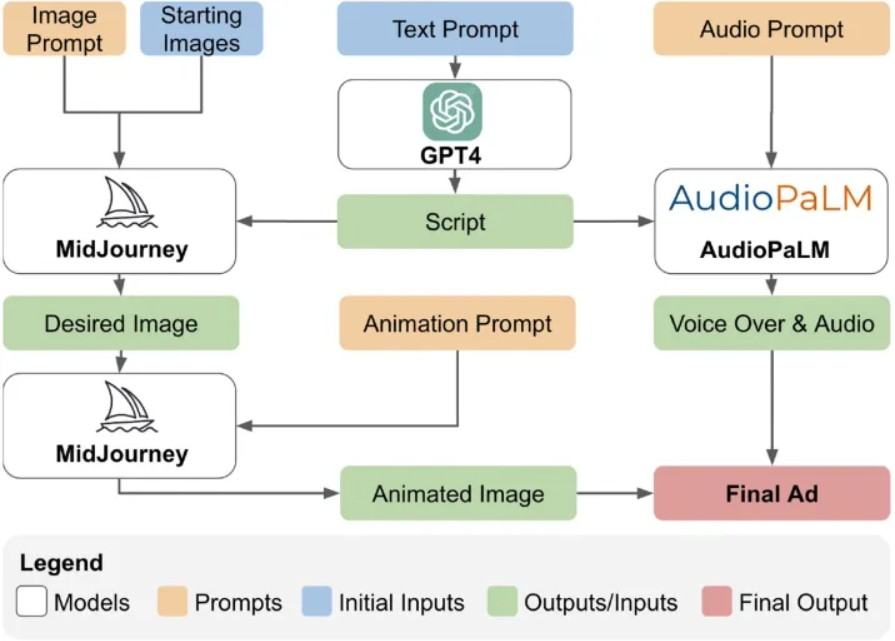
\includegraphics[width=0.85\textwidth]{images/alvarez2023_workflow.jpg}
        \caption[Flujo de trabajo para generación y análisis de contenido político con LLMs]{Flujo de trabajo para la generación y análisis de contenido político mediante LLMs en el contexto de campañas electorales.\\
            Fuente: \cite{pr_alvarez2023llm_political}. \citetitle{pr_alvarez2023llm_political}. (p. 4)}
        \label{fig:alvarez2023}
    \end{center}
\end{figure}
 
Se concluyó que los LLMs representan una herramienta transformadora para la ciencia política computacional, con aplicaciones directas en la clasificación de polaridad política, el monitoreo de narrativas electorales y la detección de discurso de odio en ecosistemas digitales.
 
% ──────────────────────────────────────────────────────────────
%  ANTECEDENTE 2
% ──────────────────────────────────────────────────────────────
\cite{pr_gujral2024llm_elections} publicaron el artículo titulado \citetitle{pr_gujral2024llm_elections}, el cual traducido al español significa «¿Pueden los LLMs Ayudar a Predecir Elecciones? Evidencia (Contraria) de la Democracia más Grande del Mundo».
 
El problema abordado fue la limitación de los métodos convencionales de encuestas de opinión y \textit{exit polls} para capturar en tiempo real la dinámica del sentimiento público en contextos electorales masivos y lingüísticamente diversos. Los autores se preguntaron si los LLMs podían superar a estas metodologías tradicionales al predecir resultados electorales mediante el análisis de grandes volúmenes de publicaciones en redes sociales. El objetivo fue evaluar la capacidad predictiva de LLMs de código abierto aplicados al análisis de sentimientos en tweets relacionados con elecciones legislativas estatales en la India.
 
De acuerdo a la metodología seguida por los autores, se recolectaron publicaciones de la plataforma X (antes Twitter) relacionadas con diferentes elecciones estatales en India. Se aplicaron dos LLMs de código abierto —Llama~2 y Zephyr— mediante técnicas de \textit{prompting} para clasificar el sentimiento de los tweets hacia cada partido político, sin recurrir a \textit{fine-tuning}. Los resultados de sentimiento fueron agregados para generar predicciones de resultados electorales, las cuales fueron comparadas directamente con los resultados reales y con predicciones de encuestas tradicionales. La Figura \ref{fig:gujral2024} muestra la comparación entre las predicciones del modelo LLM y los resultados electorales reales en los estados analizados.
 
\begin{figure}[!ht]
    \begin{center}
        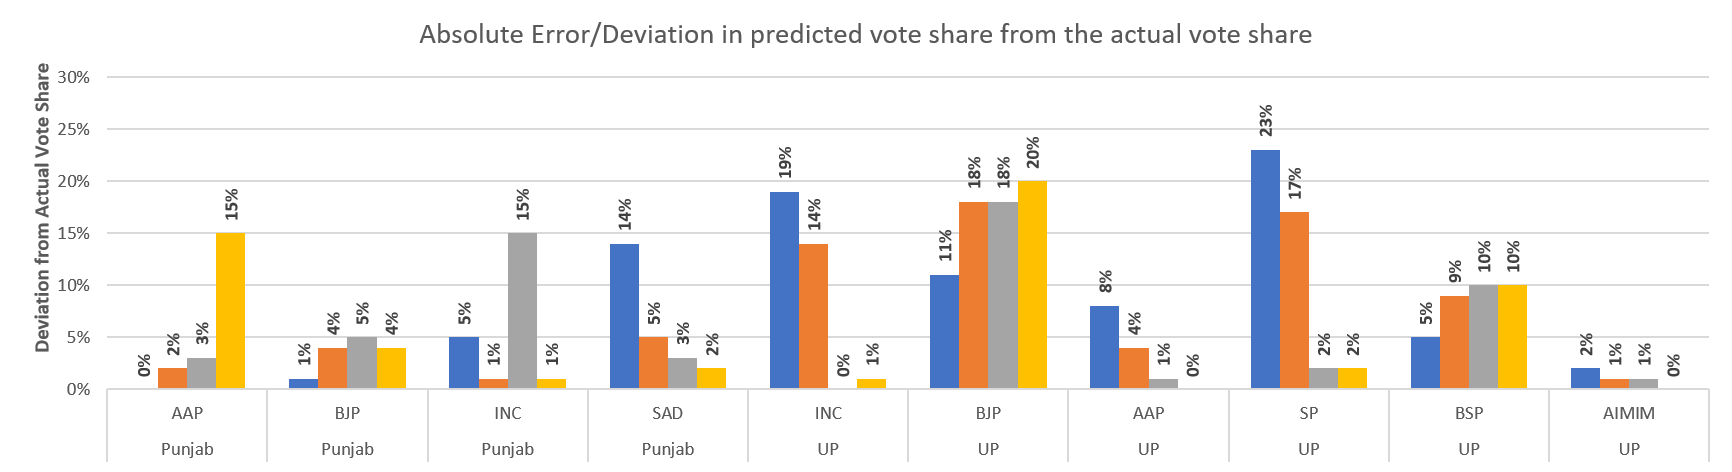
\includegraphics[width=0.82\textwidth]{images/gujral2024_predictions.png}
        \caption[Comparación entre predicciones del modelo LLM y resultados electorales reales en estados de India]{Comparación entre las predicciones basadas en análisis de sentimientos con LLMs y los resultados electorales reales en distintos estados de India.\\
            Fuente: \cite{pr_gujral2024llm_elections}. \citetitle{pr_gujral2024llm_elections}. (p. 6)}
        \label{fig:gujral2024}
    \end{center}
\end{figure}
 
Los resultados mostraron que los modelos basados en LLMs lograron predicciones más cercanas a los resultados electorales reales que los \textit{exit polls} y encuestas de opinión tradicionales en varios de los estados analizados. Sin embargo, también se identificaron limitaciones importantes, como la baja penetración de internet en ciertas regiones y la diversidad lingüística del electorado, factores que restringen la representatividad de los datos de redes sociales.
 
Se concluyó que el análisis de sentimientos con LLMs constituye una perspectiva novedosa y prometedora para la inteligencia electoral, aunque su aplicabilidad varía según el contexto sociocultural y el nivel de digitalización de la población.
 
% ──────────────────────────────────────────────────────────────
%  ANTECEDENTE 3
% ──────────────────────────────────────────────────────────────
\cite{pr_mendonca2025bertopic_political} publicaron el artículo titulado \citetitle{pr_mendonca2025bertopic_political}, el cual traducido al español significa «Modelado del Discurso Político con Sentence-BERT y BERTopic».
 
El problema central identificado por los autores fue la ausencia de metodologías capaces de rastrear dinámicamente la evolución de los temas en el discurso político digital, y de medir la influencia de los valores morales en su longevidad. Ante la limitación de modelos estáticos de detección de temas como LDA, los autores se propusieron diseñar un marco de evolución temática que integre modelos de embeddings semánticos con teorías del comportamiento político. El objetivo fue analizar la duración y las dimensiones morales de los temas presentes en la actividad de Twitter del 117.º Congreso de los Estados Unidos.
 
Según la metodología empleada por los autores, se recolectaron tweets publicados por miembros del Congreso durante el período legislativo estudiado. Se aplicaron embeddings semánticos mediante el modelo Sentence-BERT (variante \textit{all-MiniLM-L6-v2}) para representar el contenido de cada tweet en un espacio vectorial de alta dimensión. Posteriormente, se realizó reducción de dimensionalidad con UMAP y clustering con HDBSCAN dentro del framework BERTopic, permitiendo la detección automática de temas sin necesidad de definir previamente su número. Para rastrear la evolución temporal, se implementó el módulo de \textit{dynamic topic modeling} de BERTopic, que segmenta los datos en ventanas de tiempo y re-entrena las representaciones de cada período. Finalmente, se integró la Teoría de Fundamentos Morales (MFT) para medir qué valores morales dominan en los temas más duraderos. La arquitectura del marco de trabajo propuesto se ilustra en la Figura \ref{fig:mendonca2025}.
 
\begin{figure}[!ht]
    \begin{center}
        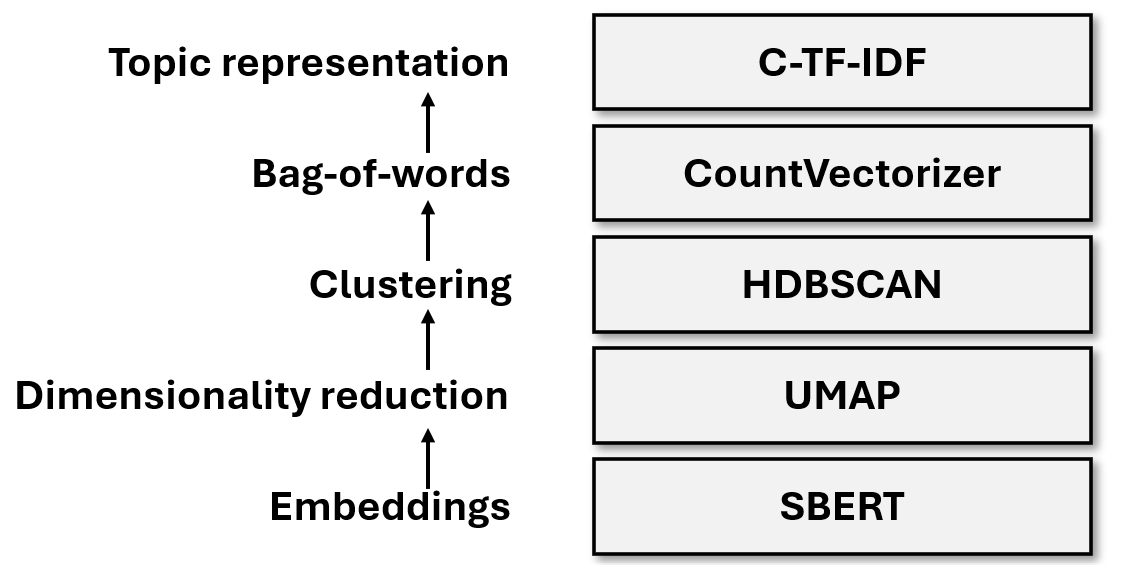
\includegraphics[width=0.88\textwidth]{images/mendonca2025_framework.png}
        \caption[Marco de trabajo para detección dinámica de temas y análisis de fundamentos morales en Twitter político]{Marco de trabajo para la detección dinámica de temas con BERTopic y el análisis de fundamentos morales aplicado al discurso político en Twitter.\\
            Fuente: \cite{pr_mendonca2025bertopic_political}. \citetitle{pr_mendonca2025bertopic_political}. (p. 5)}
        \label{fig:mendonca2025}
    \end{center}
\end{figure}
 
Los resultados revelaron que, si bien los temas generales tienden a permanecer estables a lo largo del tiempo, los temas más granulares se disuelven rápidamente, limitando su influencia en el discurso político sostenido. Además, se encontró que los fundamentos morales de «Cuidado» y «Lealtad» predominan en los temas de mayor longevidad, mientras que las diferencias partidarias se manifiestan en distintas estrategias de encuadre moral.
 
Se concluyó que la integración de BERTopic con marcos teóricos como la MFT permite una comprensión más profunda de las dinámicas del discurso político en ecosistemas digitales, siendo una metodología directamente aplicable a sistemas de inteligencia electoral que requieran monitoreo de narrativas en tiempo real.
 
% ──────────────────────────────────────────────────────────────
%  ANTECEDENTE 4
% ──────────────────────────────────────────────────────────────
\cite{pr_janssens2025bertopic_llm} publicaron el artículo titulado \citetitle{pr_janssens2025bertopic_llm}, el cual traducido al español significa «Reducción de Temas Asistida por LLMs para BERTopic en Datos de Redes Sociales».
 
El problema abordado fue que el framework BERTopic, aunque efectivo para la extracción de temas a partir de grandes corpus, genera un número excesivo de temas semánticamente superpuestos cuando se aplica a datos de redes sociales, caracterizados por ser cortos, ruidosos y dispersos. Esta proliferación de temas redundantes dificulta la interpretación de los resultados y limita la utilidad práctica del modelo en contextos de monitoreo político. El objetivo fue desarrollar un método de reducción de temas automático, interpretable, reproducible y escalable que combine las fortalezas de BERTopic con la capacidad semántica de los LLMs.
 
Según la metodología empleada por los autores, el proceso se diseñó en dos etapas principales. En la primera, BERTopic genera un conjunto inicial de temas mediante embeddings de transformers y clustering con HDBSCAN. Cada tema es representado por sus diez palabras clave principales (extraídas mediante c-TF-IDF) o por una etiqueta generada por un LLM. En la segunda etapa, estas representaciones son entregadas como entrada a un LLM, que recibe instrucciones para identificar y fusionar iterativamente los temas semánticamente similares hasta alcanzar un número objetivo de temas. Se evaluaron cuatro LLMs distintos: GPT-4o-mini, Llama3-8b, Gemma3-12b y Qwen3-30b-a3b, aplicados sobre tres datasets de redes sociales: tweets de Trump, tweets de COVID-19 y tweets de ciberbullying. La Figura \ref{fig:janssens2025} ilustra el pipeline propuesto por los autores, comparando el proceso de reducción asistida por LLM frente al método estándar de BERTopic.
 
\begin{figure}[!ht]
    \begin{center}
        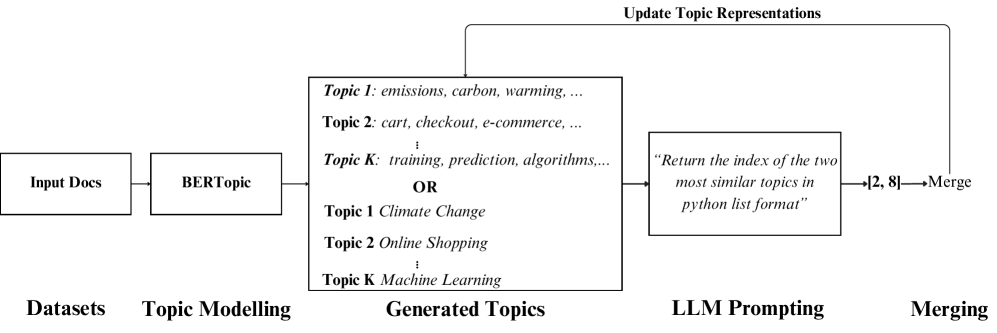
\includegraphics[width=0.90\textwidth]{images/janssens2025_pipeline.png}
        \caption[Pipeline de reducción de temas asistida por LLMs combinada con BERTopic para datos de redes sociales]{Pipeline propuesto que combina BERTopic para la generación inicial de temas y LLMs para la reducción iterativa de temas superpuestos en datos de redes sociales.\\
            Fuente: \cite{pr_janssens2025bertopic_llm}. \citetitle{pr_janssens2025bertopic_llm}. (p. 4)}
        \label{fig:janssens2025}
    \end{center}
\end{figure}
 
Los resultados evidenciaron mejoras significativas en coherencia y diversidad temática respecto al método interno de reducción de BERTopic (parámetro \texttt{nr\_topics}), siendo GPT-4o-mini el modelo que obtuvo los resultados más consistentes en los tres datasets evaluados. El método propuesto demostró ser reproducible y metodológicamente transparente, resolviendo una importante brecha en la literatura de modelado de temas para datos de redes sociales.
 
Se concluyó que la integración de LLMs como asistentes de reducción temática en el pipeline de BERTopic constituye una solución viable y escalable para el análisis de grandes volúmenes de datos políticos digitales, con aplicaciones directas en sistemas de detección dinámica de temas electorales.
 
% ──────────────────────────────────────────────────────────────
%  ANTECEDENTE 5
% ──────────────────────────────────────────────────────────────
\cite{pr_chen2024combating_misinformation} publicaron el artículo titulado \citetitle{pr_chen2024combating_misinformation} en la revista \textit{AI Magazine}, el cual traducido al español significa «Combatiendo la Desinformación en la Era de los LLMs: Oportunidades y Desafíos».
 
El problema central abordado por los autores fue el crecimiento exponencial de la desinformación en plataformas digitales, especialmente en contextos electorales, y la insuficiencia de los métodos tradicionales de detección —basados en características lingüísticas y redes de propagación— para hacer frente a la velocidad y sofisticación del contenido falso generado en la actualidad. El objetivo fue mapear sistemáticamente el rol dual de los LLMs en el ecosistema de la desinformación: como amenaza potencial al ser capaces de generar noticias falsas convincentes, y como herramienta de defensa al poder detectarlas y verificarlas de manera automatizada.
 
Según la metodología empleada por los autores, se realizó una revisión sistemática de la literatura reciente sobre detección y generación de desinformación mediante LLMs. Se construyeron y analizaron datasets de noticias falsas generadas por modelos como GPT-3.5, evaluando la dificultad de su detección tanto por humanos como por sistemas automáticos. Asimismo, se examinaron arquitecturas de verificación basadas en \textit{retrieval-augmented generation} (RAG) y técnicas de \textit{fact-checking} automatizado. La Figura \ref{fig:chen2024} muestra el marco conceptual de oportunidades y desafíos identificado por los autores en torno al uso de LLMs para combatir la desinformación.
 
\begin{figure}[!ht]
    \begin{center}
        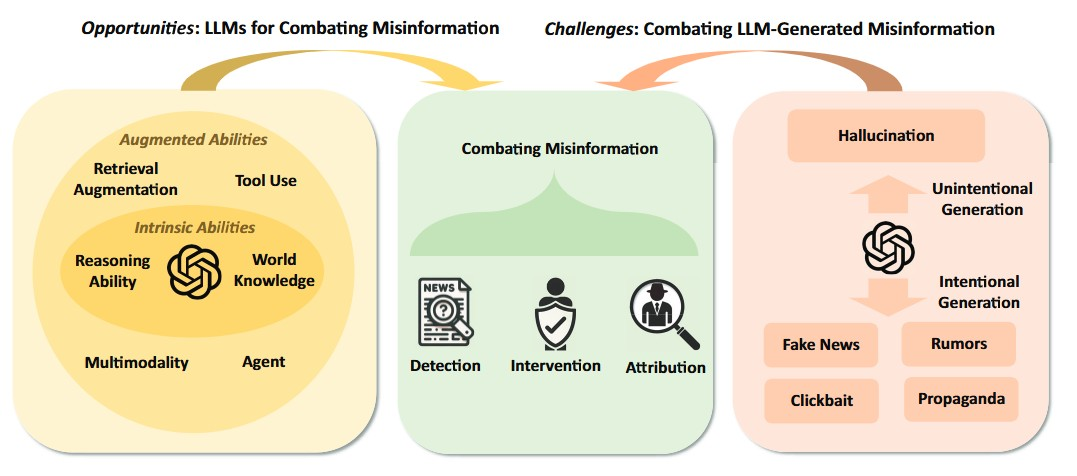
\includegraphics[width=0.80\textwidth]{images/chen2024_framework.jpg}
        \caption[Marco conceptual de oportunidades y desafíos de los LLMs en la detección de desinformación electoral]{Marco conceptual que ilustra el rol dual de los LLMs como generadores y detectores de desinformación en procesos electorales.\\
            Fuente: \cite{pr_chen2024combating_misinformation}. \citetitle{pr_chen2024combating_misinformation}. (p. 3)}
        \label{fig:chen2024}
    \end{center}
\end{figure}
 
Los resultados del estudio mostraron que los LLMs de última generación, como GPT-4, alcanzan alta precisión en la detección de noticias falsas incluso cuando el contenido falso fue generado después de su fecha de corte de conocimiento, lo que sugiere que los modelos aprenden patrones estilísticos y argumentativos del contenido desinformativo más allá de su conocimiento factual. Sin embargo, también se identificaron vulnerabilidades importantes: el contenido falso generado por LLMs resulta significativamente más difícil de detectar que el generado por humanos, tanto para sistemas automáticos como para lectores humanos.
 
Se concluyó que la integración de módulos de verificación basados en LLMs es fundamental en cualquier sistema de inteligencia electoral que analice la percepción pública en ecosistemas digitales, dado que la desinformación condiciona directamente la opinión ciudadana y los resultados de las encuestas en línea.
 
% ──────────────────────────────────────────────────────────────
%  ANTECEDENTE 6
% ──────────────────────────────────────────────────────────────
\cite{pr_alvi2023twitter_election_review} publicaron el artículo titulado \citetitle{pr_alvi2023twitter_election_review} en la revista \textit{PeerJ Computer Science}, cuya traducción en nuestro idioma es «En las Fronteras de los Datos de Twitter y el Análisis de Sentimientos en la Predicción Electoral: Una Revisión».
 
El problema identificado fue la ausencia de una síntesis comprehensiva y actualizada que integre los avances en NLP, aprendizaje automático y datos de redes sociales para la predicción de resultados electorales. A pesar del crecimiento sostenido de publicaciones en este campo, existía una brecha en la sistematización de metodologías, fuentes de datos y métricas de evaluación utilizadas. El objetivo de los autores fue evaluar el estado del arte de forma sistemática, identificando tendencias, enfoques dominantes, limitaciones recurrentes y vacíos en la literatura sobre predicción electoral mediante análisis de sentimientos en Twitter.
 
Según la metodología empleada por los autores, se realizó una revisión sistemática de la literatura, seleccionando y analizando estudios relevantes sobre predicción electoral con datos de Twitter. Se examinaron trabajos que utilizaron enfoques que van desde clasificadores léxicos y SVM hasta redes neuronales profundas y modelos basados en transformers como BERT y RoBERTa. Para cada estudio se documentó el conjunto de datos utilizado, el método de análisis de sentimientos, el modelo de predicción y las métricas de evaluación reportadas. La Figura \ref{fig:alvi2023} muestra la evolución cronológica de los enfoques metodológicos identificados en la revisión, desde métodos léxicos hasta LLMs.
 
\begin{figure}[!ht]
    \begin{center}
        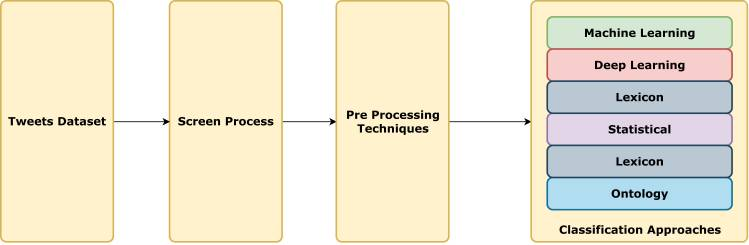
\includegraphics[width=0.85\textwidth]{images/alvi2023_evolution.jpg}
        \caption[Evolución cronológica de los enfoques de análisis de sentimientos para predicción electoral en Twitter]{Evolución de los enfoques metodológicos en la predicción electoral mediante análisis de sentimientos en Twitter, desde métodos léxicos hasta modelos de lenguaje de gran escala.\\
            Fuente: \cite{pr_alvi2023twitter_election_review}. \citetitle{pr_alvi2023twitter_election_review}. (p. 8)}
        \label{fig:alvi2023}
    \end{center}
\end{figure}
 
Los resultados de la revisión evidenciaron una evolución sostenida hacia modelos de mayor precisión: los clasificadores basados en SVM lograron exactitudes entre el 66\% y el 86\%, mientras que los modelos de aprendizaje profundo y los basados en transformers alcanzaron rangos de exactitud del 86\% al 97\% según el contexto electoral analizado. Se identificó además que la incorporación de características de sentimiento, más allá del mero volumen de menciones, mejora consistentemente el poder predictivo de los modelos.
 
Se concluyó que la combinación de análisis de sentimientos con técnicas de NLP avanzado constituye una línea de investigación madura y en plena expansión, con aplicaciones directas en sistemas de inteligencia electoral. Este trabajo valida la pertinencia del enfoque metodológico adoptado en la presente investigación.
 
% ──────────────────────────────────────────────────────────────
%  ANTECEDENTE 7
% ──────────────────────────────────────────────────────────────
\cite{pr_islam2025latent_topic} publicaron el artículo titulado \citetitle{pr_islam2025latent_topic}, el cual traducido al español significa «Síntesis Latente de Temas: Aprovechando los LLMs para el Análisis de Publicidad Electoral».
 
El problema abordado fue la incapacidad de los modelos de tópicos tradicionales —como LDA y el propio BERTopic sin supervisión semántica— para capturar estructuras discursivas latentes y jerarquías temáticas complejas en grandes corpus dinámicos de publicidad política en redes sociales. Los autores se preguntaron si era posible construir automáticamente, sin intervención humana ni conjunto semilla inicial, una taxonomía coherente e interpretable de temas políticos a partir de datos no etiquetados de campañas electorales. El objetivo fue desarrollar un framework de síntesis temática iterativa basado en LLMs para analizar las estrategias de publicidad política en redes sociales durante las elecciones presidenciales de los Estados Unidos de 2024.
 
Según la metodología empleada por los autores, se construyó y publicó un dataset curado de anuncios de campaña de las elecciones presidenciales de 2024. El proceso metodológico se estructuró en múltiples etapas: primero, se realizaron embeddings de los anuncios y se aplicó clustering de densidad siguiendo el enfoque de BERTopic. Luego, en lugar de generar etiquetas con c-TF-IDF, se utilizó un LLM para producir etiquetas semánticamente ricas para cada cluster. A continuación, el framework construye iterativamente una taxonomía de temas, partiendo de cero y fusionando o refinando etiquetas en cada iteración hasta alcanzar una estructura jerárquica coherente, sin requerir un conjunto de temas predefinido. La arquitectura completa del framework propuesto se ilustra en la Figura \ref{fig:islam2025}.
 
\begin{figure}[!ht]
    \begin{center}
        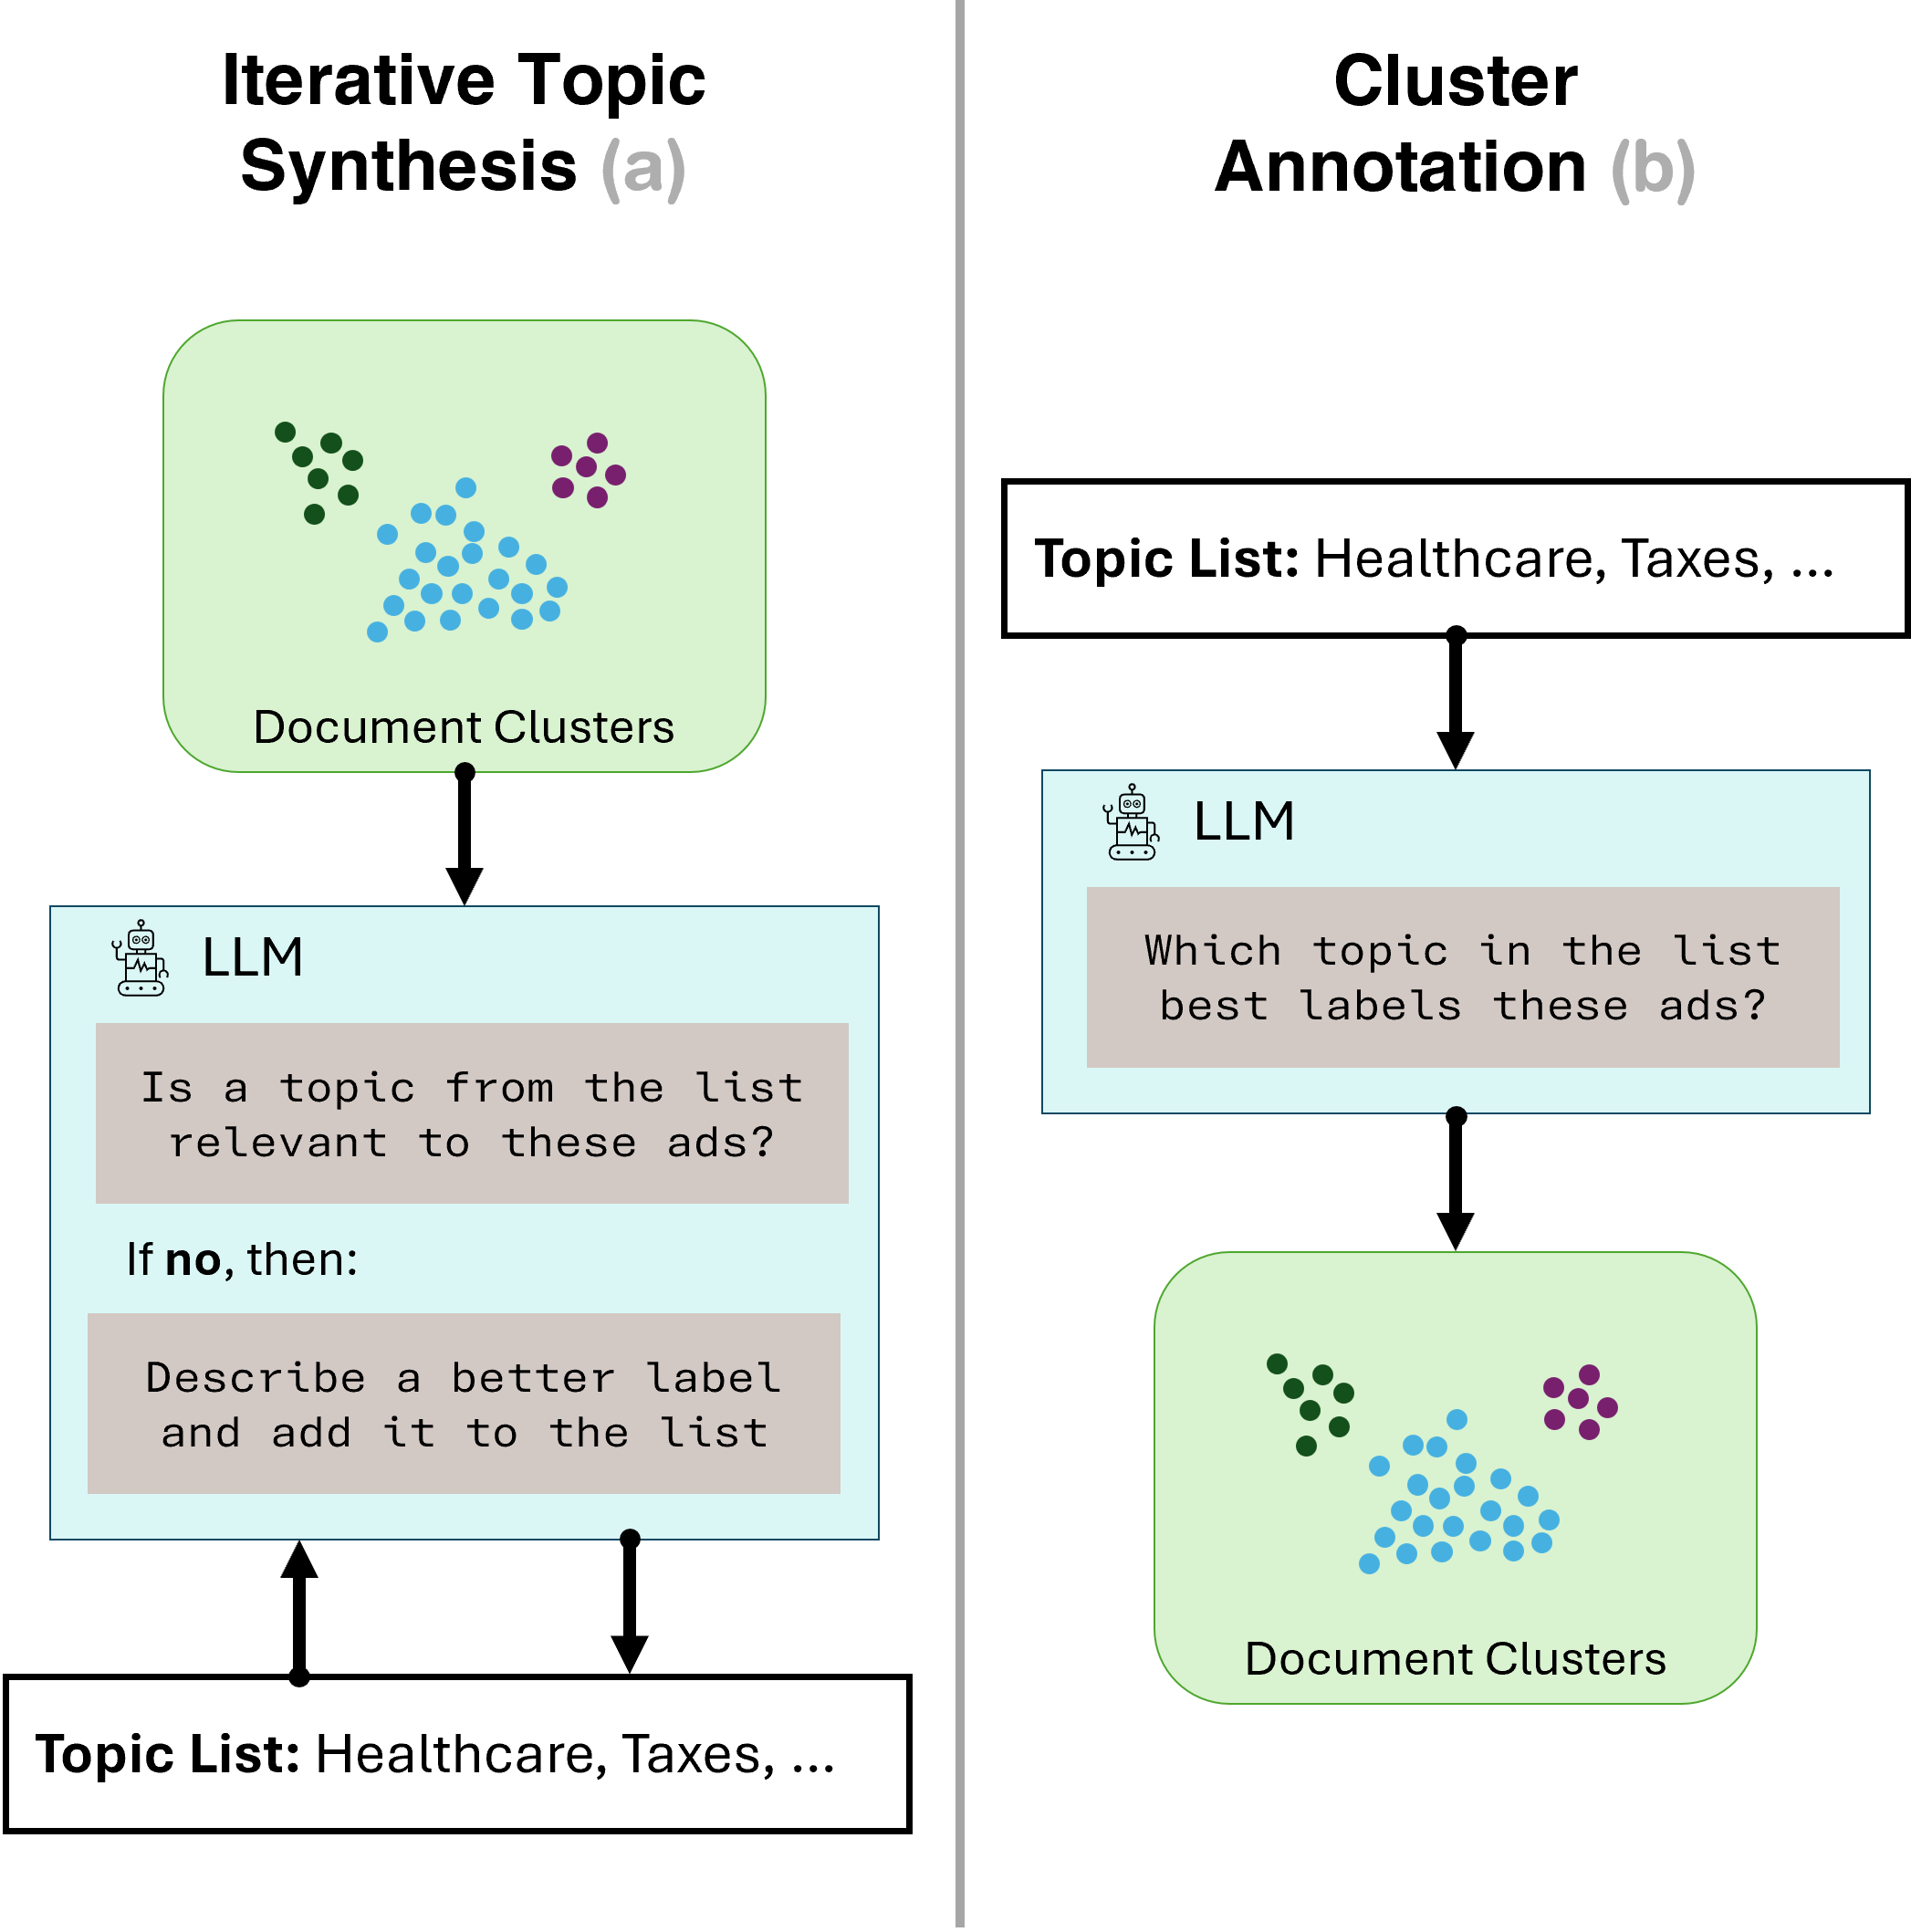
\includegraphics[width=0.92\textwidth]{images/islam2025_architecture.png}
        \caption[Arquitectura del framework de síntesis temática iterativa con LLMs para análisis de publicidad política]{Arquitectura del framework de síntesis de temas latentes mediante LLMs, aplicado al análisis de publicidad política en las elecciones presidenciales de EE.UU. 2024.\\
            Fuente: \cite{pr_islam2025latent_topic}. \citetitle{pr_islam2025latent_topic}. (p. 4)}
        \label{fig:islam2025}
    \end{center}
\end{figure}
 
Los resultados de la evaluación demostraron que el mecanismo de síntesis iterativa produce etiquetas de temas más consistentes y mejor alineadas con el juicio humano que los modelos clásicos de tópicos y que el etiquetado directo mediante LLMs en un único paso (\textit{single-shot}). Anotadores expertos en ciencias sociales computacionales validaron cualitativamente la coherencia y granularidad de la taxonomía generada, confirmando su utilidad para el análisis de estrategias de microfocalización electoral.
 
Se concluyó que este framework de síntesis temática iterativa es altamente aplicable a sistemas de monitoreo electoral en tiempo real, donde la identificación rápida y automática de temas emergentes —sin necesidad de etiquetado manual previo— representa una ventaja fundamental. Este trabajo es directamente relevante para la presente investigación, ya que valida la viabilidad de construir sistemas de inteligencia electoral capaces de detectar dinámicamente los temas relevantes que moldean la percepción pública nacional en ecosistemas digitales.

\section{Bases Teóricas}

% ──────────────────────────────────────────────────────────────
\subsection{Inteligencia Artificial}
% ──────────────────────────────────────────────────────────────
 
La Inteligencia Artificial (IA) se define como la capacidad de las máquinas para ejecutar procesos inteligentes, donde un agente “inteligente” ideal percibe su entorno y actúa de manera que maximiza sus probabilidades de alcanzar un objetivo \parencite{bk_russell2009intart}. Este concepto se emplea cuando un sistema es capaz de imitar funciones cognitivas propias del ser humano, como el aprendizaje y la resolución de problemas \parencite{bk_russell2004intart}.

A lo largo de la historia se han seguido cuatro grandes enfoques: dos centrados en el comportamiento humano y dos enfocados en la racionalidad. El enfoque empírico nace con la prueba propuesta por Alan Turing en 1950, cuyo computador debía contar con capacidades de procesamiento de lenguaje natural, representación del conocimiento, razonamiento automático y aprendizaje automático. Si el evaluador incluía además una señal de video, la prueba pasaba a denominarse Prueba Global de Turing, sumando también visión computacional y robótica. Por su parte, el enfoque racional se fundamenta en las «leyes del pensamiento» enunciadas por filósofos griegos como Aristóteles, derivando en el estudio de la lógica y, posteriormente, en la tradición logista de la IA.
 
En la actualidad, la Inteligencia Artificial (IA) posee diversas aplicaciones, entre las que destacan la minería de datos, el procesamiento de lenguaje natural (PLN), la robótica y los videojuegos. Asimismo, comprende distintas ramas como el aprendizaje automático, la visión computacional y los modelos de lenguaje de gran escala, siendo estas últimas de particular interés para la presente investigación.
 
% ──────────────────────────────────────────────────────────────
\subsection{Aprendizaje Automático}
% ──────────────────────────────────────────────────────────────
 
El Aprendizaje Automático (\textit{Machine Learning}) es una disciplina de la Inteligencia Artificial orientada al desarrollo de métodos que permitan a las computadoras aprender a partir de los datos, mediante la identificación de algoritmos y heurísticas que transforman ejemplos en modelos, sin requerir una programación explícita \parencite{bk_russell2009intart}. Sus algoritmos integran diversas tecnologías —como el aprendizaje profundo, las redes neuronales y el procesamiento de lenguaje natural— las cuales funcionan a partir de patrones y conocimientos extraídos de datos previos \parencite{bk_alpaydin2014ml}.

Entre los principales enfoques de aprendizaje se encuentran el supervisado, el no supervisado y el aprendizaje por refuerzo. En el \textbf{aprendizaje supervisado}, se emplean datos etiquetados con el objetivo de construir una función que relacione entradas con salidas esperadas. Este tipo se divide en dos categorías: la regresión, que produce valores numéricos continuos, y la clasificación, que asigna elementos a clases definidas. Por su parte, el \textbf{aprendizaje no supervisado} utiliza datos sin etiquetar para identificar estructuras ocultas en la información, comúnmente mediante técnicas de agrupamiento o \textit{clustering}. Finalmente, el \textbf{aprendizaje por refuerzo} se basa en la interacción de un agente con su entorno, donde aprende a tomar decisiones a partir de una retroalimentación en forma de recompensas, optimizando así su comportamiento con el tiempo.
 
% ──────────────────────────────────────────────────────────────
\subsection{Aprendizaje Profundo}
% ──────────────────────────────────────────────────────────────
 
El Aprendizaje Profundo (\textit{Deep Learning}) es una subárea del Aprendizaje Automático que permite a las computadoras ejecutar tareas asociadas a capacidades humanas, como el reconocimiento de imágenes o del lenguaje, mediante el ajuste de parámetros y el entrenamiento de sistemas capaces de aprender de forma autónoma a través de múltiples capas de procesamiento \parencite{gl_sas_deeplearning}. Este enfoque se fundamenta en principios inspirados en el funcionamiento del cerebro humano, utilizando redes neuronales artificiales de gran escala.

A diferencia del Aprendizaje Automático tradicional, el Aprendizaje Profundo integra en un mismo proceso la extracción de características y la clasificación, mientras que en los métodos convencionales estas etapas se desarrollan de manera separada. Esta propiedad lo posiciona como la base tecnológica de los Modelos de Lenguaje de Gran Escala, los cuales constituyen el eje central de la presente investigación.
 
% ──────────────────────────────────────────────────────────────
\subsection{Procesamiento del Lenguaje Natural}
% ──────────────────────────────────────────────────────────────
 
El Procesamiento del Lenguaje Natural (\textit{Natural Language Processing}, NLP) es un área interdisciplinaria que integra la lingüística computacional, las ciencias de la computación, la ciencia cognitiva y la inteligencia artificial. Su propósito es estudiar cómo las computadoras pueden comprender y procesar el lenguaje humano para llevar a cabo diversas tareas, como el reconocimiento de voz, el análisis léxico, la generación automática de resúmenes, el análisis de sentimientos y la identificación de temas \parencite{bk_deng2018deeplearningnlp}.
 
Desde una perspectiva histórica, el NLP ha evolucionado a través de tres olas. El \textbf{Racionalismo} (décadas de 1960 a 1980) se fundamentó en reglas gramaticales diseñadas por expertos, basándose en la concepción del lenguaje como una facultad innata propuesta por Noam Chomsky. El \textbf{Empirismo} se caracterizó por la explotación de grandes corpus de texto mediante Aprendizaje Automático, con modelos como el Modelo Oculto de Markov (HMM). El \textbf{Aprendizaje Profundo}, como tercera y actual ola, emplea redes neuronales de múltiples capas entrenadas sobre volúmenes masivos de texto, permitiendo capturar dependencias semánticas complejas que los enfoques anteriores no podían modelar \parencite{bk_deng2018deeplearningnlp}.
 
Para el presente trabajo, el NLP constituye la disciplina madre que sustenta todas las técnicas aplicadas: el análisis de sentimientos, la detección de temas y los modelos de lenguaje de gran escala.
 
\subsubsection{Representación Vectorial del Texto}
 
Antes de aplicar cualquier modelo de NLP, el texto debe ser transformado en representaciones numéricas. Entre las modalidades más usadas se encuentran las siguientes.
 
La \textbf{Bolsa de Palabras} (\textit{Bag-of-Words} o BoW) es una técnica de extracción de características que representa los textos a partir de un vocabulario predefinido, contabilizando la frecuencia de aparición de cada término, sin tomar en cuenta el orden ni la estructura de las palabras dentro del documento \parencite{bk_brownlee2017deeplearning_nlp}. La \textbf{Frecuencia del Término - Frecuencia Inversa del Documento} (\textit{TF-IDF}) resalta las palabras más significativas en el corpus al combinar la frecuencia de aparición de un término en un documento con la penalización de términos que aparecen en demasiados documentos, calculada mediante la Ecuación \ref{eq:tfidf_llm}:
 
\begin{equation}\label{eq:tfidf_llm}
\phantomsection
TF\text{-}IDF_{(t,d)} = TF_{(t,d)} \times \log\frac{N}{df_{(t)}}
\end{equation}
\myequations{Fórmula de TF-IDF para ponderación de términos}
 
Donde $TF_{(t,d)}$ es la frecuencia del término $t$ en el documento $d$, $N$ es el número total de documentos y $df_{(t)}$ es el número de documentos que contienen el término $t$.
 
La \textbf{Incrustación de Palabras} (\textit{Word Embedding}) representa las palabras como vectores densos de baja dimensionalidad en un espacio vectorial continuo, donde palabras con significados similares tienen representaciones cercanas. Algoritmos como Word2Vec \parencite{tec_mikolov2013word2vec} y GloVe \parencite{gl_pennington2014glove} popularizaron este enfoque. Sin embargo, estas representaciones son estáticas, es decir, una misma palabra tiene siempre el mismo vector independientemente del contexto en que aparezca. Los modelos de transformers, descritos más adelante, resuelven esta limitación al generar representaciones contextuales dinámicas.
 
% ──────────────────────────────────────────────────────────────
\subsection{La Arquitectura Transformer}
% ──────────────────────────────────────────────────────────────
 
La arquitectura Transformer, introducida por \cite{tec_vaswani2017attention} en el influyente artículo titulado «\textit{Attention Is All You Need}», representa el fundamento arquitectónico de todos los modelos de lenguaje modernos de gran escala. A diferencia de las Redes Neuronales Recurrentes (RNN) y las Redes de Memoria Larga a Corto Plazo (LSTM), el Transformer prescinde de la recurrencia y procesa la secuencia de entrada completa en paralelo mediante un mecanismo denominado \textit{self-attention} (auto-atención), lo que permite capturar dependencias de largo alcance entre palabras de manera mucho más eficiente.
 
\subsubsection{Mecanismo de Atención}
 
El mecanismo central del Transformer es la \textbf{atención multi-cabeza} (\textit{multi-head attention}). Este mecanismo calcula, para cada token (unidad léxica) de la secuencia, cuánta «atención» debe prestarse a cada otro token al momento de construir su representación. Formalmente, la atención se define mediante la Ecuación \ref{eq:attention}:
 
\begin{equation}\label{eq:attention}
\phantomsection
\text{Attention}(Q, K, V) = \text{softmax}\left(\frac{QK^T}{\sqrt{d_k}}\right)V
\end{equation}
\myequations{Fórmula del mecanismo de atención escalada por producto punto}
 
Donde:
\begin{conditions}
Q   & matriz de consultas (\textit{queries}) \\
K   & matriz de claves (\textit{keys}) \\
V   & matriz de valores (\textit{values}) \\
d_k & dimensión de los vectores de claves
\end{conditions}
 
El producto $QK^T$ mide la similitud entre cada par de tokens; dividir entre $\sqrt{d_k}$ estabiliza los gradientes durante el entrenamiento; y la función \textit{softmax} convierte los puntajes en una distribución de probabilidad sobre todos los tokens. Finalmente, los valores $V$ son ponderados por estos pesos de atención. Este proceso se ejecuta en paralelo para múltiples «cabezas» de atención, cada una aprendiendo distintos tipos de relaciones semánticas y sintácticas entre los tokens.
 
\subsubsection{Arquitectura Encoder-Decoder}
 
El Transformer original sigue una arquitectura codificador-decodificador (\textit{encoder-decoder}), ilustrada en la Figura \ref{fig:transformer_arch}. El \textbf{codificador} (\textit{encoder}) procesa la secuencia de entrada y genera representaciones contextuales de alta dimensión. El \textbf{decodificador} (\textit{decoder}) toma estas representaciones junto con la secuencia generada hasta el momento para producir el siguiente token de salida, de manera autoregresiva.
 
\begin{figure}[!ht]
    \begin{center}
        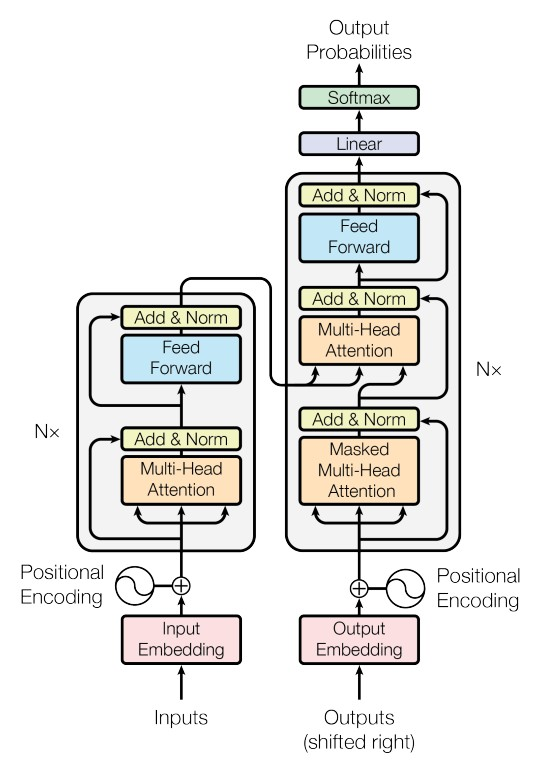
\includegraphics[width=0.70\textwidth]{images/transformer_architecture.jpg}
        \caption[Arquitectura original del Transformer con codificador y decodificador]{Arquitectura original del modelo Transformer, compuesta por un codificador (izquierda) y un decodificador (derecha), cada uno formado por capas de atención multi-cabeza y redes de retroalimentación.\\
            Fuente: \cite{tec_vaswani2017attention}. \textit{Attention Is All You Need}. (p. 3)}
        \label{fig:transformer_arch}
    \end{center}
\end{figure}
 
Existen variantes especializadas: los modelos \textbf{solo-encoder} (como BERT) son óptimos para tareas de comprensión y clasificación de texto, los modelos \textbf{solo-decoder} (como GPT) son óptimos para generación de texto, y los modelos \textbf{encoder-decoder} (como T5) son ideales para tareas de transformación de secuencias como la traducción automática o el resumen. Esta distinción es fundamental para comprender la familia de LLMs utilizados en la presente investigación.
 
% ──────────────────────────────────────────────────────────────
\subsection{Modelos de Lenguaje de Gran Escala (LLMs)}
% ──────────────────────────────────────────────────────────────
 
Los Modelos de Lenguaje de Gran Escala (\textit{Large Language Models}, LLMs) son modelos basados en la arquitectura Transformer, pre-entrenados sobre corpus de texto de escala masiva —que pueden abarcar billones de tokens— con el objetivo de aprender representaciones ricas y generalizables del lenguaje \parencite{bk_russell2009intart}. Su denominación como «de gran escala» hace referencia tanto al volumen de datos de entrenamiento como al número de parámetros del modelo, que en los casos más avanzados supera los 100 mil millones.
 
\subsubsection{Pre-entrenamiento y Ajuste Fino}
 
El ciclo de vida de un LLM comprende dos etapas principales. En la etapa de \textbf{pre-entrenamiento}, el modelo aprende a predecir tokens a partir de grandes corpus no etiquetados mediante objetivos de aprendizaje auto-supervisado, como la predicción de la siguiente palabra (\textit{next-token prediction}) en modelos GPT o el enmascaramiento de tokens (\textit{masked language modeling}) en modelos BERT \parencite{tec_devlin2018bert}. Esta etapa dota al modelo de conocimiento lingüístico y factual amplio pero general.
 
En la etapa de \textbf{ajuste fino} (\textit{fine-tuning}), el modelo pre-entrenado se re-entrena sobre un conjunto de datos etiquetado y específico de la tarea objetivo —como clasificación de sentimientos políticos o detección de temas electorales— adaptando sus parámetros al dominio concreto de aplicación. Existe además el ajuste fino con instrucciones (\textit{instruction fine-tuning}) y con retroalimentación humana (\textit{Reinforcement Learning from Human Feedback}, RLHF), técnicas que han sido clave en la alineación de modelos como GPT-4 y Claude \parencite{tec_ouyang2022instructgpt}.
 
\subsubsection{Aprendizaje por Contexto: Zero-shot y Few-shot}
 
Una capacidad emergente de los LLMs de gran escala es el \textbf{aprendizaje por contexto} (\textit{in-context learning}), que permite al modelo realizar nuevas tareas sin actualizar sus parámetros, simplemente incluyendo ejemplos o instrucciones en el \textit{prompt} (texto de entrada). Se distinguen dos modalidades principales, representadas en la Figura \ref{fig:zeroshot_fewshot}:
 
\begin{figure}[!ht]
    \begin{center}
        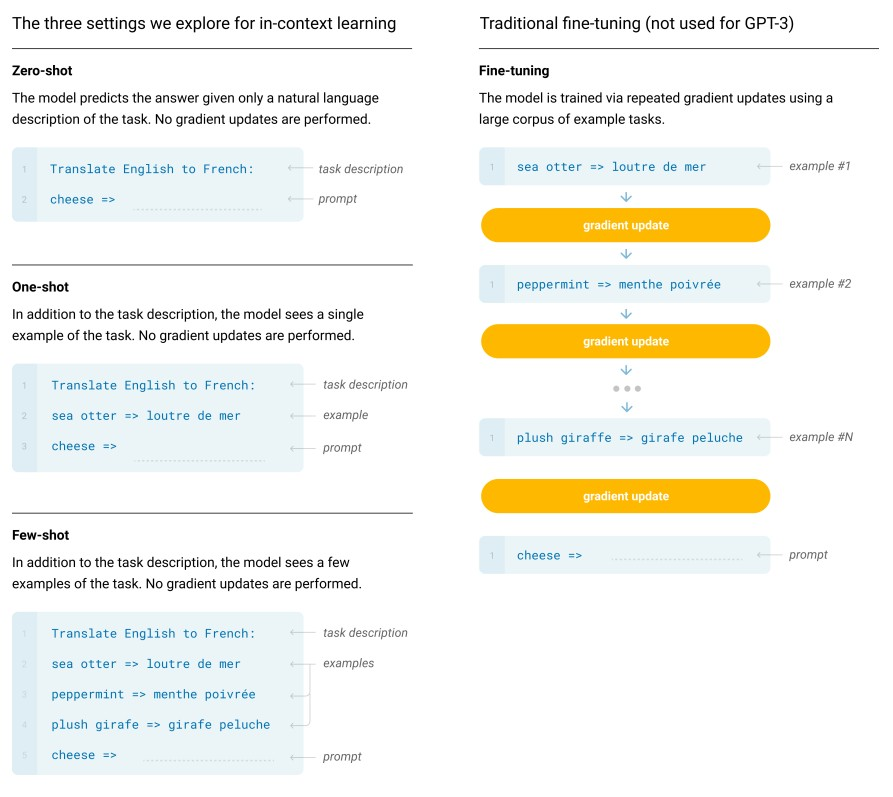
\includegraphics[width=0.88\textwidth]{images/zeroshot_fewshot.jpg}
        \caption[Comparación entre los enfoques zero-shot, one-shot y few-shot en LLMs]{Comparación entre los paradigmas zero-shot, one-shot y few-shot para el aprendizaje por contexto en modelos de lenguaje de gran escala.\\
            Fuente: \cite{tec_brown2020gpt3}. \textit{Language Models are Few-Shot Learners}. (p. 7)}
        \label{fig:zeroshot_fewshot}
    \end{center}
\end{figure}
 
\begin{itemize}
    \item \textbf{Zero-shot}: El modelo realiza la tarea sin recibir ningún ejemplo previo, únicamente con una descripción de la tarea en el \textit{prompt}. Esta modalidad es especialmente útil cuando no se dispone de datos etiquetados en el dominio objetivo.
    \item \textbf{Few-shot}: El modelo recibe un pequeño número de ejemplos etiquetados en el \textit{prompt} antes de procesar la consulta real. Esta modalidad mejora significativamente el desempeño en tareas especializadas sin necesidad de re-entrenamiento.
\end{itemize}
 
Ambas modalidades son fundamentales en la presente investigación, ya que permiten aplicar LLMs al análisis de discurso político sin requerir grandes conjuntos de datos etiquetados en español.
 
\subsubsection{Modelos LLM Relevantes para la Investigación}
 
Varios LLMs son directamente relevantes para los objetivos de esta tesis:
 
\textbf{BERT} (\textit{Bidirectional Encoder Representations from Transformers}), propuesto por \cite{tec_devlin2018bert}, es un modelo solo-encoder que introduce el pre-entrenamiento bidireccional, permitiendo capturar el contexto tanto izquierdo como derecho de cada token simultáneamente. Ha sido ampliamente adoptado para clasificación de sentimientos y tareas de comprensión textual.
 
\textbf{DeepSeek} es una familia de modelos de lenguaje desarrollada por la empresa china DeepSeek AI, cuya variante \textit{deepseek-chat} ha demostrado capacidades competitivas con modelos de frontera a una fracción del costo operacional \parencite{tec_deepseek2024}. Una característica técnica diferenciadora es su mecanismo de caché de prefijo (\textit{prompt prefix caching}), que almacena en memoria el prefijo invariante del prompt —catálogos de entidades, instrucciones y ejemplos few-shot— y lo reutiliza entre llamadas, reduciendo el costo efectivo de tokens de entrada hasta en un 75\% cuando la tasa de \textit{cache hit} es alta. En el sistema implementado se observó una tasa de \textit{cache hit} sostenida del 85.5\%, lo que hizo de DeepSeek la opción económicamente más viable para el procesamiento masivo de corpus electorales.

\textbf{RoBERTa} (\textit{Robustly Optimized BERT Pretraining Approach}) es una versión optimizada de BERT que emplea mayor volumen de datos y elimina el objetivo de predicción de oración siguiente (\textit{next sentence prediction}), logrando mejoras significativas en benchmarks de NLP \parencite{tec_liu2019roberta}.
 
\textbf{GPT} (\textit{Generative Pre-trained Transformer}) es una familia de modelos solo-decoder desarrollados por OpenAI, ampliamente utilizados como referencia en investigación de LLMs debido a sus capacidades emergentes de razonamiento y aprendizaje few-shot \parencite{tec_brown2020gpt3}.

\textbf{Llama} es una familia de LLMs de código abierto desarrollada por Meta AI \parencite{tec_touvron2023llama}, que ha democratizado la investigación con LLMs al ofrecer modelos de alto rendimiento sin restricciones de acceso. Su variante Llama~2 ha sido ampliamente utilizada en estudios de análisis político descritos en los antecedentes de esta investigación.
 
La Figura \ref{fig:llm_timeline} ilustra la evolución cronológica de los principales LLMs desde 2018 hasta la actualidad, evidenciando la aceleración en el desarrollo de estos modelos y el exponencial crecimiento en su número de parámetros.
 
\begin{figure}[!ht]
    \begin{center}
        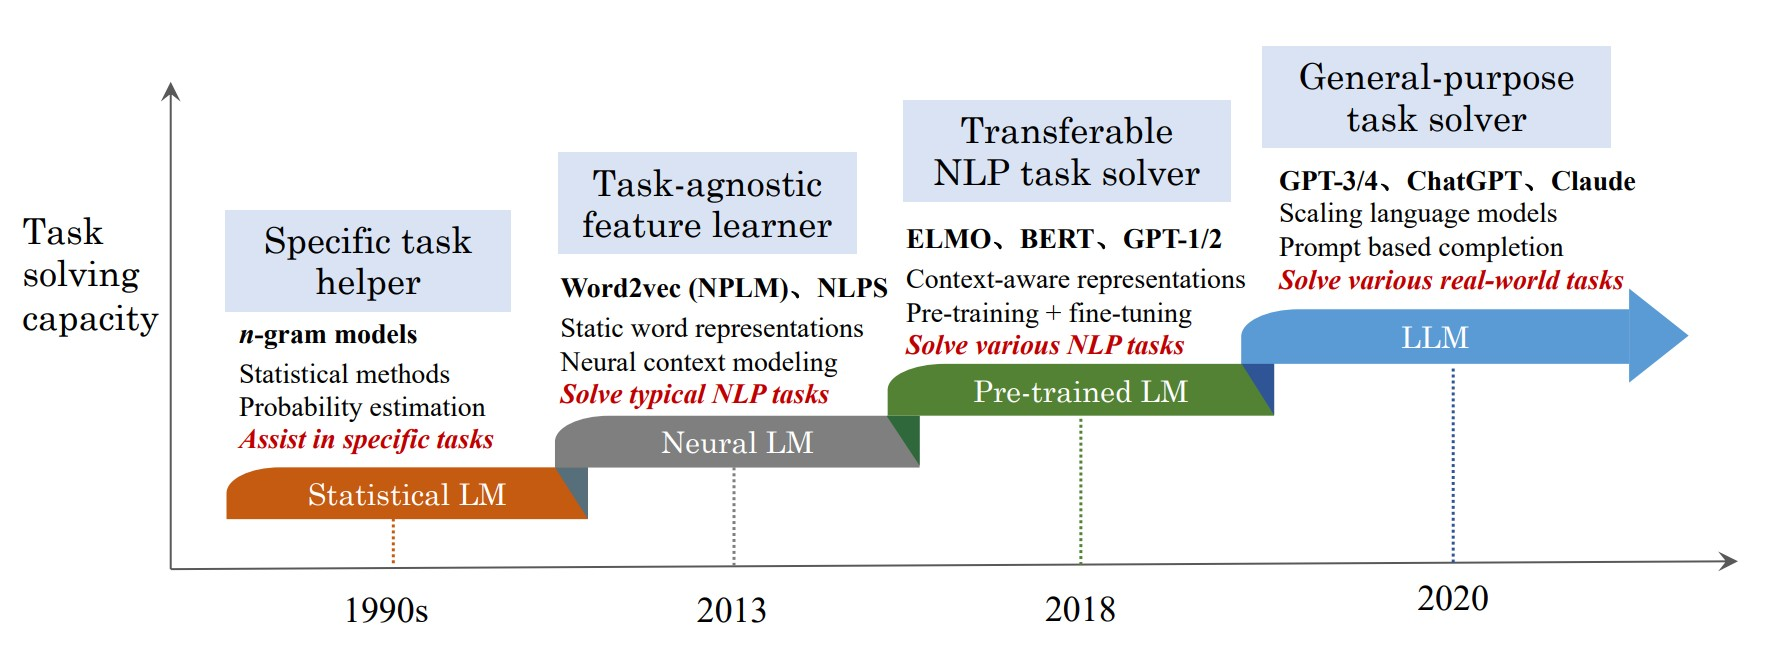
\includegraphics[width=0.92\textwidth]{images/llm_timeline.jpg}
        \caption[Evolución cronológica de los principales modelos de lenguaje de gran escala]{Línea de tiempo de los principales LLMs, mostrando el crecimiento exponencial en número de parámetros y capacidades.\\
        Fuente: \cite{tec_zhao2023llm_survey}. \citetitle{tec_zhao2023llm_survey}. (p. 2)}
        \label{fig:llm_timeline}
    \end{center}
\end{figure}
 
% ──────────────────────────────────────────────────────────────
\subsection{Análisis de Sentimientos}
% ──────────────────────────────────────────────────────────────
 
El análisis de sentimientos, también denominado minería de opiniones (\textit{opinion mining}), es la tarea de NLP orientada a identificar y extraer información subjetiva de textos, determinando si el contenido expresa una actitud positiva, negativa o neutral hacia una entidad, persona, evento o tema \parencite{tec_liu2012sentiment}. En el contexto de la inteligencia electoral, esta tarea permite medir la percepción pública hacia candidatos, partidos políticos y políticas públicas a partir de grandes volúmenes de publicaciones en ecosistemas digitales.
 
\subsubsection{Niveles de Análisis}
 
El análisis de sentimientos puede realizarse en distintos niveles de granularidad, como podemos ver en la Figura \ref{fig:sentiment_levels}:
 
\begin{figure}[!ht]
    \begin{center}
        \includegraphics[width=0.85\textwidth]{images/sentiment_levels.jpg}
        \caption[Niveles de granularidad del análisis de sentimientos]{Niveles de análisis de sentimientos: a nivel de documento, a nivel de oración y a nivel de aspecto, con sus respectivos ejemplos de aplicación en textos políticos.\\
            Fuente: Elaboración propia basada en \cite{tec_liu2012sentiment}.}
        \label{fig:sentiment_levels}
    \end{center}
\end{figure}
 
\begin{itemize}
    \item \textbf{Nivel de documento}: Se asigna una polaridad global al documento completo. Es el nivel más simple pero pierde información sobre aspectos específicos mencionados en el texto.
    \item \textbf{Nivel de oración}: Se analiza el sentimiento de cada oración de forma independiente, permitiendo una granularidad mayor.
    \item \textbf{Nivel de aspecto} (\textit{Aspect-Based Sentiment Analysis}, ABSA): Se identifica el sentimiento expresado hacia entidades o aspectos específicos mencionados en el texto. Por ejemplo, en un tweet sobre una campaña electoral, se puede detectar sentimiento positivo hacia la propuesta económica de un candidato y negativo hacia su gestión en seguridad.
\end{itemize}
 
\subsubsection{Enfoques Metodológicos}
 
Los principales enfoques para el análisis de sentimientos son los siguientes:
 
El \textbf{enfoque basado en léxicos} utiliza diccionarios de palabras con polaridad pre-asignada (por ejemplo, VADER, SentiWordNet, AFINN) para calcular el sentimiento de un texto mediante la suma de las puntuaciones de sus palabras. Es rápido y no requiere datos de entrenamiento, pero tiene dificultades con el lenguaje figurado, la ironía y el sarcasmo, tan frecuentes en el discurso político.
 
El \textbf{enfoque basado en aprendizaje automático supervisado} entrena clasificadores como Naive Bayes, SVM o Regresión Logística sobre conjuntos de datos etiquetados. Supera al anterior en precisión pero requiere datos etiquetados en el dominio y el idioma objetivo.
 
El \textbf{enfoque basado en Aprendizaje Profundo y LLMs} utiliza modelos como BERT, RoBERTa o GPT para generar representaciones contextuales del texto, logrando los mejores resultados en la actualidad. La Figura \ref{fig:sentiment_comparison} ilustra la comparación de rendimiento entre estos enfoques en tareas de análisis de sentimientos políticos.
 
\begin{figure}[!ht]
    \begin{center}
        \includegraphics[width=0.82\textwidth]{images/sentiment_comparison.jpg}
        \caption[Comparación de rendimiento entre enfoques de análisis de sentimientos en texto político]{Comparación de exactitud entre los enfoques léxico, aprendizaje automático clásico y modelos basados en LLMs para análisis de sentimientos en texto político en redes sociales.\\
            Fuente: Elaboración propia basada en \cite{tec_liu2012sentiment} y \cite{pr_alvarez2023llm_political}.}
        \label{fig:sentiment_comparison}
    \end{center}
\end{figure}
 
\subsubsection{Desafíos en el Análisis de Sentimientos Político}
 
El análisis de sentimientos aplicado al discurso político en ecosistemas digitales presenta desafíos específicos que los métodos convencionales no resuelven satisfactoriamente. En primer lugar, el \textbf{lenguaje figurado}: la ironía, el sarcasmo y el humor político son formas frecuentes de expresión en redes sociales, y su interpretación requiere comprender el contexto pragmático más allá del significado literal de las palabras. En segundo lugar, la \textbf{ambigüedad de entidades}: un mismo tweet puede expresar sentimientos positivos hacia un partido y negativos hacia otro, o referirse a múltiples figuras políticas simultáneamente. En tercer lugar, la \textbf{diversidad lingüística}: en contextos latinoamericanos, el español presenta variaciones léxicas y expresivas significativas entre países, lo que dificulta la generalización de modelos entrenados en una sola variedad. Los LLMs multilingües como XLM-RoBERTa han mostrado ventajas sustanciales para este tipo de escenarios.
 
% ──────────────────────────────────────────────────────────────
\subsection{Detección Dinámica de Temas}
% ──────────────────────────────────────────────────────────────
 
La detección de temas (\textit{topic modeling} o \textit{topic detection}) es una familia de técnicas de NLP no supervisadas cuyo objetivo es descubrir automáticamente los temas o asuntos latentes que subyacen en un corpus de documentos, sin necesidad de etiquetas previas \parencite{bk_blei2012lda}. En el contexto de la inteligencia electoral, permite identificar qué temas están siendo discutidos en el ecosistema digital político, con qué intensidad y cómo evolucionan en el tiempo.
 
\subsubsection{Modelos Probabilísticos: LDA}
 
La \textbf{Asignación Latente de Dirichlet} (\textit{Latent Dirichlet Allocation}, LDA), propuesta por \cite{bk_blei2012lda}, es el modelo de detección de temas más influyente de la era pre-transformers. LDA asume que cada documento es una mezcla de temas, y que cada tema es una distribución de probabilidad sobre palabras. El proceso generativo de LDA se representa en la Figura \ref{fig:lda_plate}.
 
\begin{figure}[!ht]
    \begin{center}
        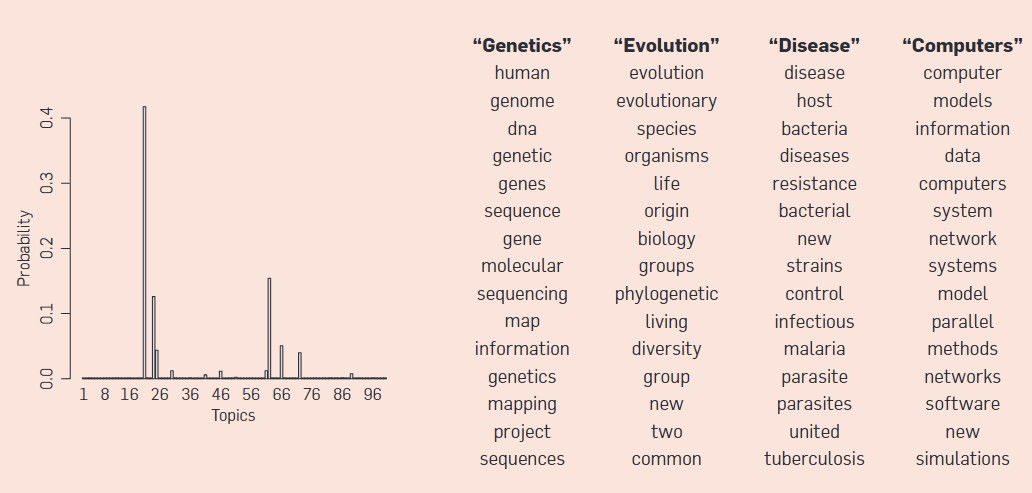
\includegraphics[width=0.70\textwidth]{images/lda_plate.jpg}
        \caption[Notación de plato del modelo LDA]{Notación de plato del modelo de Asignación Latente de Dirichlet (LDA), mostrando las distribuciones de temas por documento ($\theta$) y de palabras por tema ($\phi$), controladas por los hiperparámetros Dirichlet $\alpha$ y $\beta$.\\
            Fuente: \cite{bk_blei2012lda}. \textit{Probabilistic Topic Models}. (p. 79)}
        \label{fig:lda_plate}
    \end{center}
\end{figure}
 
Sin embargo, LDA presenta limitaciones importantes para el análisis de datos de redes sociales: sus representaciones de topics son locales y no contextuales, tiene dificultades con textos muy cortos como tweets, y no puede capturar temas emergentes en tiempo real sin re-entrenamiento completo del modelo.
 
\subsubsection{BERTopic: Modelado de Temas Neural}
 
\textbf{BERTopic}, propuesto por \cite{tec_grootendorst2022bertopic}, es un framework moderno de modelado de temas que aprovecha embeddings de transformers y clustering basado en densidad. Su pipeline se compone de cuatro etapas principales, representadas en la Figura \ref{fig:bertopic_pipeline}:
 
\begin{figure}[!ht]
    \begin{center}
        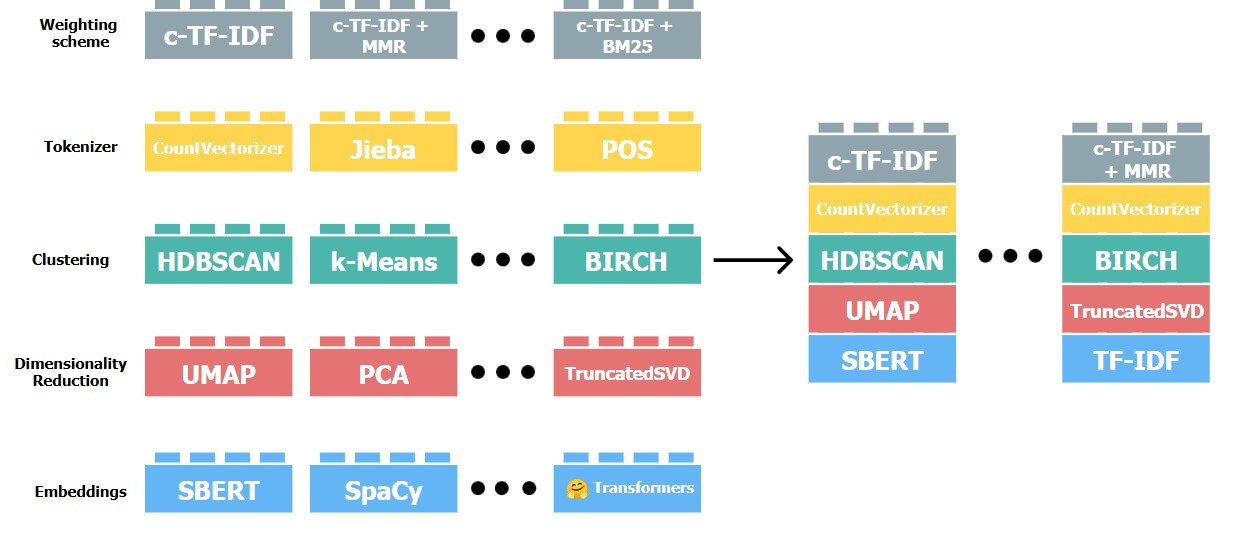
\includegraphics[width=0.90\textwidth]{images/bertopic_pipeline.jpg}
        \caption[Pipeline completo del framework BERTopic para detección de temas neurales]{Pipeline del framework BERTopic: generación de embeddings con transformers, reducción de dimensionalidad con UMAP, clustering con HDBSCAN y representación de temas con c-TF-IDF.\\
            Fuente: \cite{tec_grootendorst2022bertopic}. \textit{BERTopic: Neural Topic Modeling with a Class-Based TF-IDF Procedure}.}
        \label{fig:bertopic_pipeline}
    \end{center}
\end{figure}
 
\begin{enumerate}
    \item \textbf{Generación de embeddings}: Cada documento es transformado en un vector de alta dimensión mediante un modelo de transformers (generalmente Sentence-BERT), capturando su significado semántico completo en contexto.
    \item \textbf{Reducción de dimensionalidad}: Los embeddings de alta dimensión son reducidos mediante UMAP (\textit{Uniform Manifold Approximation and Projection}), preservando la estructura local del espacio semántico.
    \item \textbf{Clustering}: El algoritmo HDBSCAN (\textit{Hierarchical Density-Based Spatial Clustering of Applications with Noise}) agrupa los documentos en clusters sin requerir especificar el número de grupos a priori, asignando automáticamente los documentos ruidosos o atípicos a la categoría de «outliers».
    \item \textbf{Representación de temas}: Cada cluster de documentos es representado mediante una variante de c-TF-IDF (\textit{class-based TF-IDF}), que identifica las palabras más características de ese grupo de documentos en relación al resto del corpus.
\end{enumerate}
 
BERTopic supera a LDA en coherencia semántica, manejo de textos cortos y capacidad de integración con LLMs para la generación de etiquetas interpretables para cada tema \parencite{tec_grootendorst2022bertopic}.
 
\subsubsection{Detección Dinámica de Temas}
 
La \textbf{detección dinámica de temas} (\textit{dynamic topic modeling}) extiende los modelos estáticos para rastrear cómo los temas evolucionan a través del tiempo. BERTopic implementa esta capacidad mediante la segmentación temporal del corpus: los documentos se agrupan en ventanas de tiempo y se re-calculan las representaciones de topics para cada período, permitiendo visualizar la evolución de narrativas políticas en el tiempo, como se muestra en la Figura \ref{fig:dynamic_topics}.
 
\begin{figure}[!ht]
    \begin{center}
        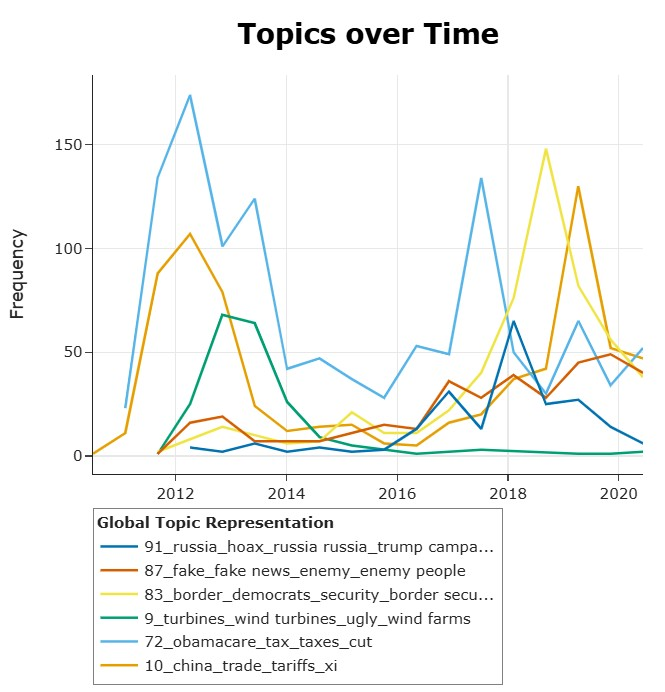
\includegraphics[width=0.88\textwidth]{images/dynamic_topics.jpg}
        \caption[Evolución temporal de temas políticos detectados mediante BERTopic dinámico]{Ejemplo de evolución temporal de temas políticos detectados mediante el módulo de topic modeling dinámico de BERTopic, mostrando la frecuencia relativa de cada tema por período de tiempo.\\
            Fuente: \cite{tec_grootendorst2022bertopic}. \textit{BERTopic: Neural Topic Modeling with a Class-Based TF-IDF Procedure}.}
        \label{fig:dynamic_topics}
    \end{center}
\end{figure}
 
Esta capacidad es fundamental para los objetivos de la presente investigación, ya que el ecosistema digital durante un proceso electoral es altamente dinámico: los temas de campaña emergen, se intensifican y decaen en función de eventos como debates, escándalos o anuncios de política pública.
 
% ──────────────────────────────────────────────────────────────
\subsection{Ingeniería de Prompts}
% ──────────────────────────────────────────────────────────────
 
La \textbf{ingeniería de \textit{prompts}} (\textit{prompt engineering}) es la disciplina que estudia el diseño y optimización de las instrucciones textuales (\textit{prompts}) que se proporcionan a los LLMs para obtener de ellos respuestas de mayor calidad, precisión y relevancia sin modificar los parámetros del modelo \parencite{tec_white2023prompt}. En el contexto de la inteligencia electoral, el diseño adecuado de prompts determina en gran medida la calidad del análisis de sentimientos y la detección de temas que produce el LLM.
 
\subsubsection{Principales Técnicas}
 
Entre las técnicas de prompting más relevantes para esta investigación se encuentran las siguientes.
 
El \textbf{Chain-of-Thought prompting} (CoT) consiste en incluir en el \textit{prompt} una cadena de pasos de razonamiento intermedios antes de la respuesta final, lo cual mejora el desempeño de los LLMs en tareas que requieren razonamiento complejo \parencite{tec_wei2022cot}. Por ejemplo, en la clasificación de sentimientos políticos, se le puede pedir al modelo que primero identifique las entidades mencionadas, luego los términos evaluativos y finalmente el sentimiento hacia cada entidad.
 
El \textbf{Role prompting} asigna al LLM un rol específico al inicio del \textit{prompt} («Eres un analista político experto en discurso electoral latinoamericano...»), orientando sus respuestas hacia el dominio de interés. Esta técnica ha demostrado ser efectiva para mejorar la precisión en tareas de análisis político \parencite{pr_alvarez2023llm_political}.
 
La \textbf{Generación Aumentada por Recuperación} (\textit{Retrieval-Augmented Generation}, RAG) complementa el \textit{prompt} con información recuperada de una base de conocimiento externa (documentos de prensa, bases de datos electorales, programas de gobierno), permitiendo al LLM razonar sobre información actualizada y específica del dominio que puede no estar en sus datos de entrenamiento \parencite{tec_lewis2020rag}. La Figura \ref{fig:rag_architecture} ilustra la arquitectura general de un sistema RAG.
 
\begin{figure}[!ht]
    \begin{center}
        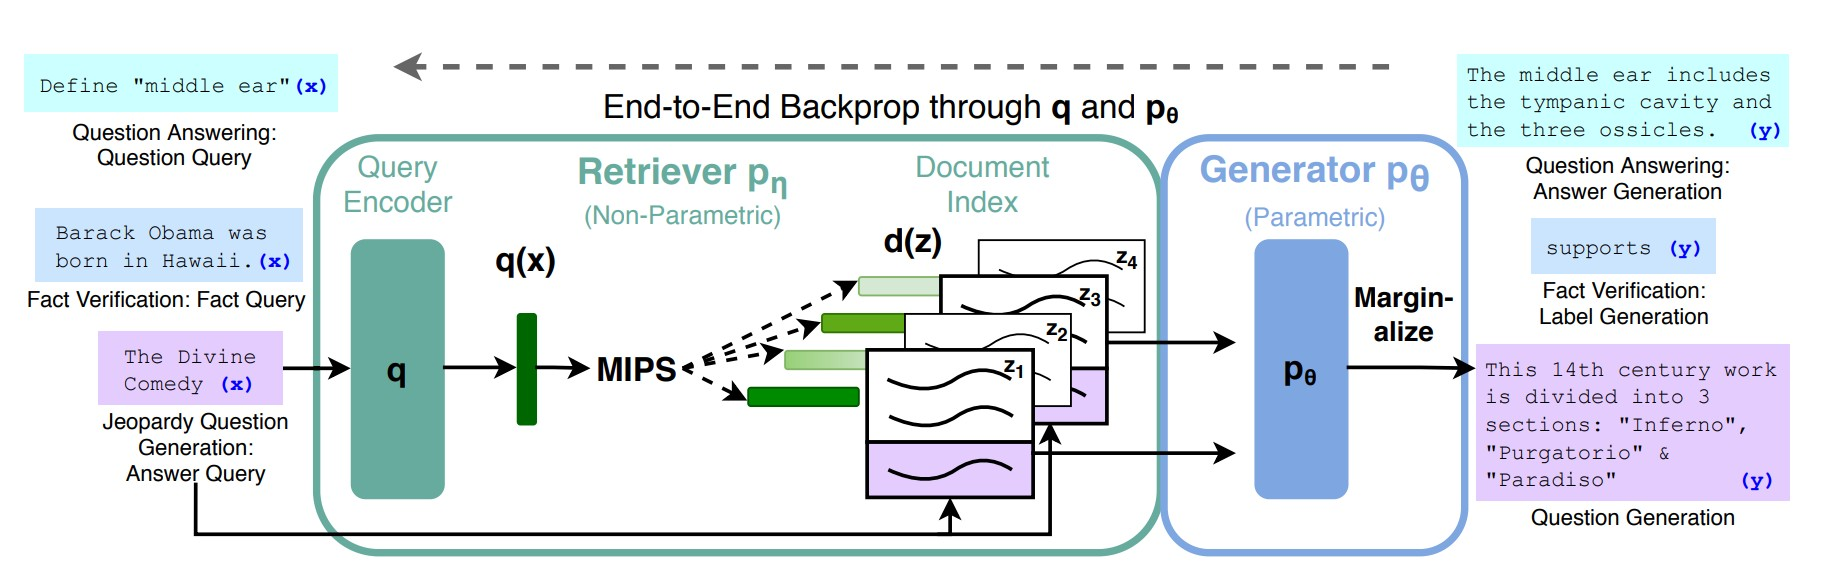
\includegraphics[width=0.88\textwidth]{images/rag_architecture.jpg}
        \caption[Arquitectura de un sistema de Generación Aumentada por Recuperación (RAG)]{Arquitectura de un sistema RAG aplicado al análisis de discurso político: el módulo de recuperación obtiene documentos relevantes de una base de conocimiento externa, que son incluidos en el \textit{prompt} junto a la consulta del usuario para que el LLM genere una respuesta fundamentada.\\
            Fuente: \cite{tec_lewis2020rag}. \textit{Retrieval-Augmented Generation for Knowledge-Intensive NLP Tasks}. (p. 3)}
        \label{fig:rag_architecture}
    \end{center}
\end{figure}
 
\subsubsection{Salida Estructurada mediante JSON}

La producción de salida estructurada (\textit{structured output}) mediante prompts es una técnica que solicita al LLM devolver respuestas exclusivamente en formato JSON válido, validable mediante esquemas Pydantic. Esta modalidad elimina la necesidad de parseo frágil y permite la integración directa del output del LLM en bases de datos relacionales \parencite{tec_white2023prompt}.

En el sistema desarrollado, cada documento es analizado con un único prompt que extrae simultáneamente: candidato protagonista, actores secundarios, tema emergente, categoría, sentimiento por candidato y nivel de confianza. Este enfoque reduce el número de llamadas al modelo, mejora la consistencia estructural de los datos y facilita el procesamiento automatizado dentro del pipeline analítico.

% ──────────────────────────────────────────────────────────────
\subsection{Ecosistemas Digitales y Redes Sociales como Fuente de Datos}
% ──────────────────────────────────────────────────────────────
 
Los \textbf{ecosistemas digitales} son entornos mediáticos complejos conformados por la interacción de múltiples plataformas digitales —redes sociales, sitios de noticias, foros, aplicaciones de mensajería— a través de las cuales los ciudadanos producen, consumen y difunden información política \parencite{tec_chadwick2013hybrid}. En el contexto electoral, estos ecosistemas constituyen la principal arena de debate político contemporáneo, superando en muchos aspectos a los medios tradicionales en velocidad, alcance e interactividad.
 
Las \textbf{redes sociales} como X (antes Twitter), Facebook, TikTok e Instagram son las fuentes de datos primarias para los sistemas de inteligencia electoral. X/Twitter, en particular, ha sido ampliamente utilizada en la investigación académica por su naturaleza pública y la disponibilidad de su API, que permite la recolección masiva de datos geolocalizados y temporalmente etiquetados \parencite{pr_alvi2023twitter_election_review}. Sus características estructurales —textos cortos (hasta 280 caracteres), hashtags, menciones de usuarios y retweets— la convierten en una fuente especialmente rica para el análisis de sentimientos y la detección de temas en tiempo real.
 
\subsubsection{Recolección y Procesamiento de Datos de Redes Sociales}
 
La recolección de datos de redes sociales para análisis electoral generalmente sigue el proceso ilustrado en la Figura \ref{fig:data_collection_pipeline}:
 
\begin{figure}[!ht]
    \begin{center}
        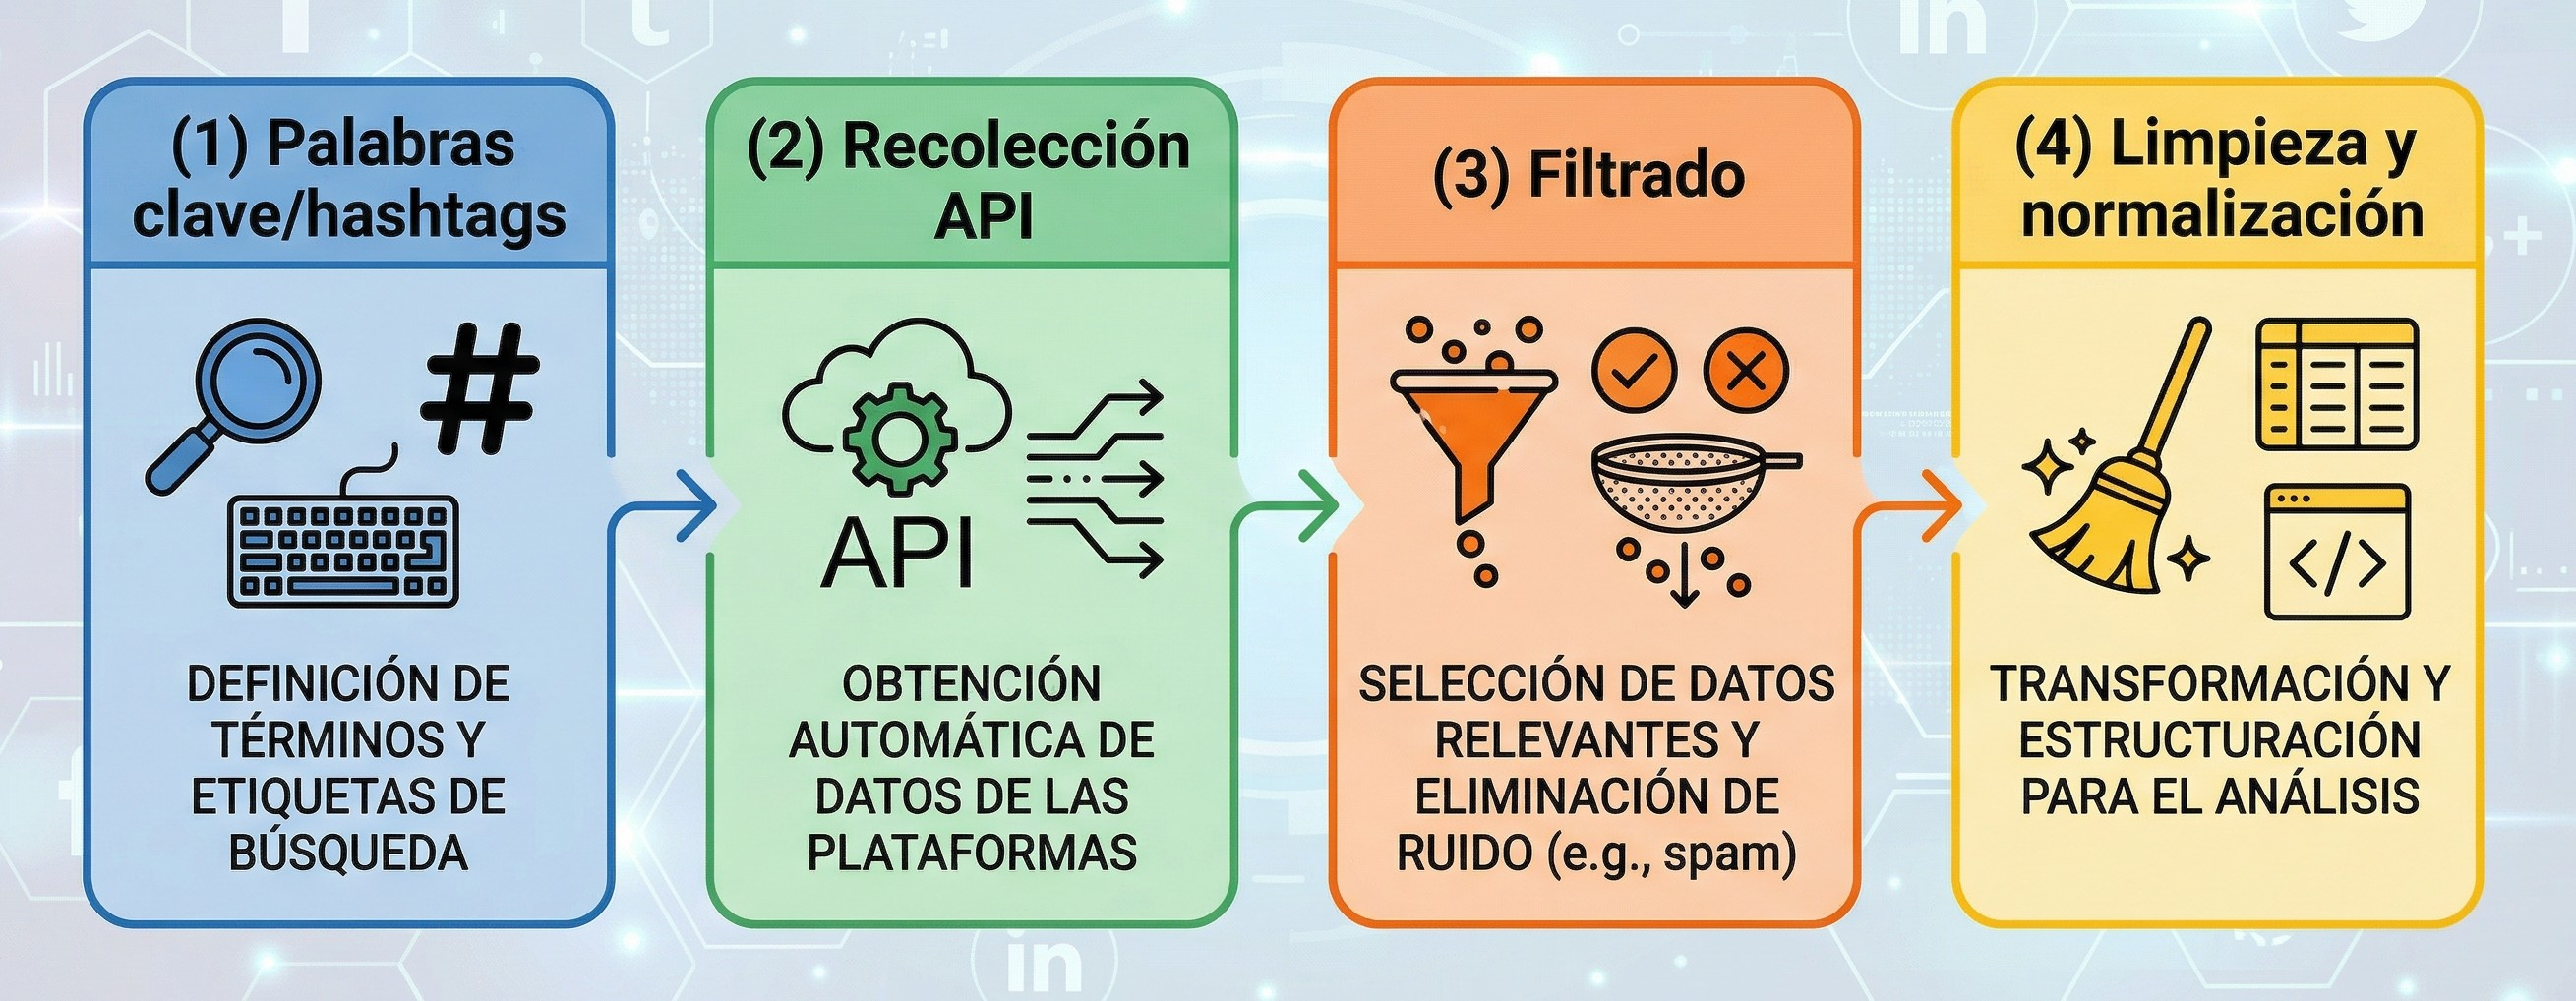
\includegraphics[width=0.85\textwidth]{images/data_collection_pipeline.jpg}
        \caption[Pipeline de recolección y preprocesamiento de datos de redes sociales para análisis electoral]{Pipeline estándar para la recolección y preprocesamiento de datos de redes sociales destinados al análisis de percepción política: definición de palabras clave, recolección vía API, filtrado, limpieza y normalización del texto.\\
            Fuente: Elaboración propia basada en \cite{pr_alvi2023twitter_election_review}.}
        \label{fig:data_collection_pipeline}
    \end{center}
\end{figure}
 
El proceso comprende las siguientes etapas: (1) \textbf{Definición de criterios de búsqueda}: selección de palabras clave, hashtags y cuentas de interés relacionadas con el proceso electoral a monitorear. (2) \textbf{Recolección vía API}: extracción de publicaciones mediante las APIs oficiales de las plataformas o herramientas de scraping. (3) \textbf{Filtrado}: eliminación de publicaciones irrelevantes, spam y bots. (4) \textbf{Limpieza y normalización}: eliminación de caracteres especiales, URLs, emojis no relevantes y normalización ortográfica.
 
\subsubsection{Detección de Desinformación en Ecosistemas Digitales}
 
Un desafío crítico en el análisis de percepción pública en ecosistemas digitales es la presencia de \textbf{desinformación} (\textit{misinformation} y \textit{disinformation}): contenido falso o engañoso que circula masivamente en redes sociales con el potencial de distorsionar la percepción ciudadana y los resultados electorales \parencite{pr_chen2024combating_misinformation}. Los LLMs representan un arma de doble filo en este contexto: por un lado, son capaces de generar contenido falso de alta calidad y difícil detección; por otro, ofrecen capacidades avanzadas de verificación automática de hechos y detección de narrativas engañosas que superan los métodos tradicionales.
 
% ──────────────────────────────────────────────────────────────
\subsection{Inteligencia Electoral}
% ──────────────────────────────────────────────────────────────
 
La \textbf{inteligencia electoral} es un campo emergente que integra técnicas de ciencia de datos, NLP e inteligencia artificial para analizar, interpretar y anticipar dinámicas del comportamiento político ciudadano a partir de múltiples fuentes de información \parencite{tec_ceron2017social}. Va más allá del simple monitoreo de redes sociales al incorporar capacidades de análisis semántico profundo, detección de patrones, seguimiento de narrativas en el tiempo y correlación con indicadores externos como encuestas de opinión y resultados electorales históricos.
 
Un sistema de inteligencia electoral integrado, como el propuesto en la presente investigación, articula los siguientes componentes, cuya interacción se ilustra en la Figura \ref{fig:electoral_intelligence_system}:
 
\begin{figure}[!ht]
    \begin{center}
        
\includegraphics[width=0.90\textwidth]{images/electoral_intelligence_system.jpg}
        \caption[Arquitectura de un sistema integrado de inteligencia electoral basado en LLMs]{Arquitectura de un sistema integrado de inteligencia electoral: recolección de datos multicanal, preprocesamiento, análisis de sentimientos con LLMs, detección dinámica de temas, detección de desinformación y visualización en tiempo real.\\
            Fuente: Elaboración propia.}
        \label{fig:electoral_intelligence_system}
    \end{center}
\end{figure}
 
\begin{itemize}
    \item \textbf{Recolección de datos multicanal}: ingesta en tiempo real de publicaciones de redes sociales, noticias digitales y foros de discusión ciudadana.
    \item \textbf{Análisis de sentimientos con LLMs}: clasificación de la polaridad (positivo, negativo, neutral) y la emoción asociada a cada publicación, desagregada por actores políticos y temas.
    \item \textbf{Detección dinámica de temas}: identificación automática y seguimiento temporal de los temas relevantes en la conversación política nacional.
    \item \textbf{Detección de desinformación}: identificación de contenido potencialmente falso o engañoso mediante técnicas de verificación basadas en LLMs.
    \item \textbf{Visualización y reporting}: dashboards interactivos que permiten a analistas políticos, periodistas e investigadores explorar los resultados del sistema en tiempo real.
\end{itemize}
 
\begin{figure}[!ht]
    \begin{center}
        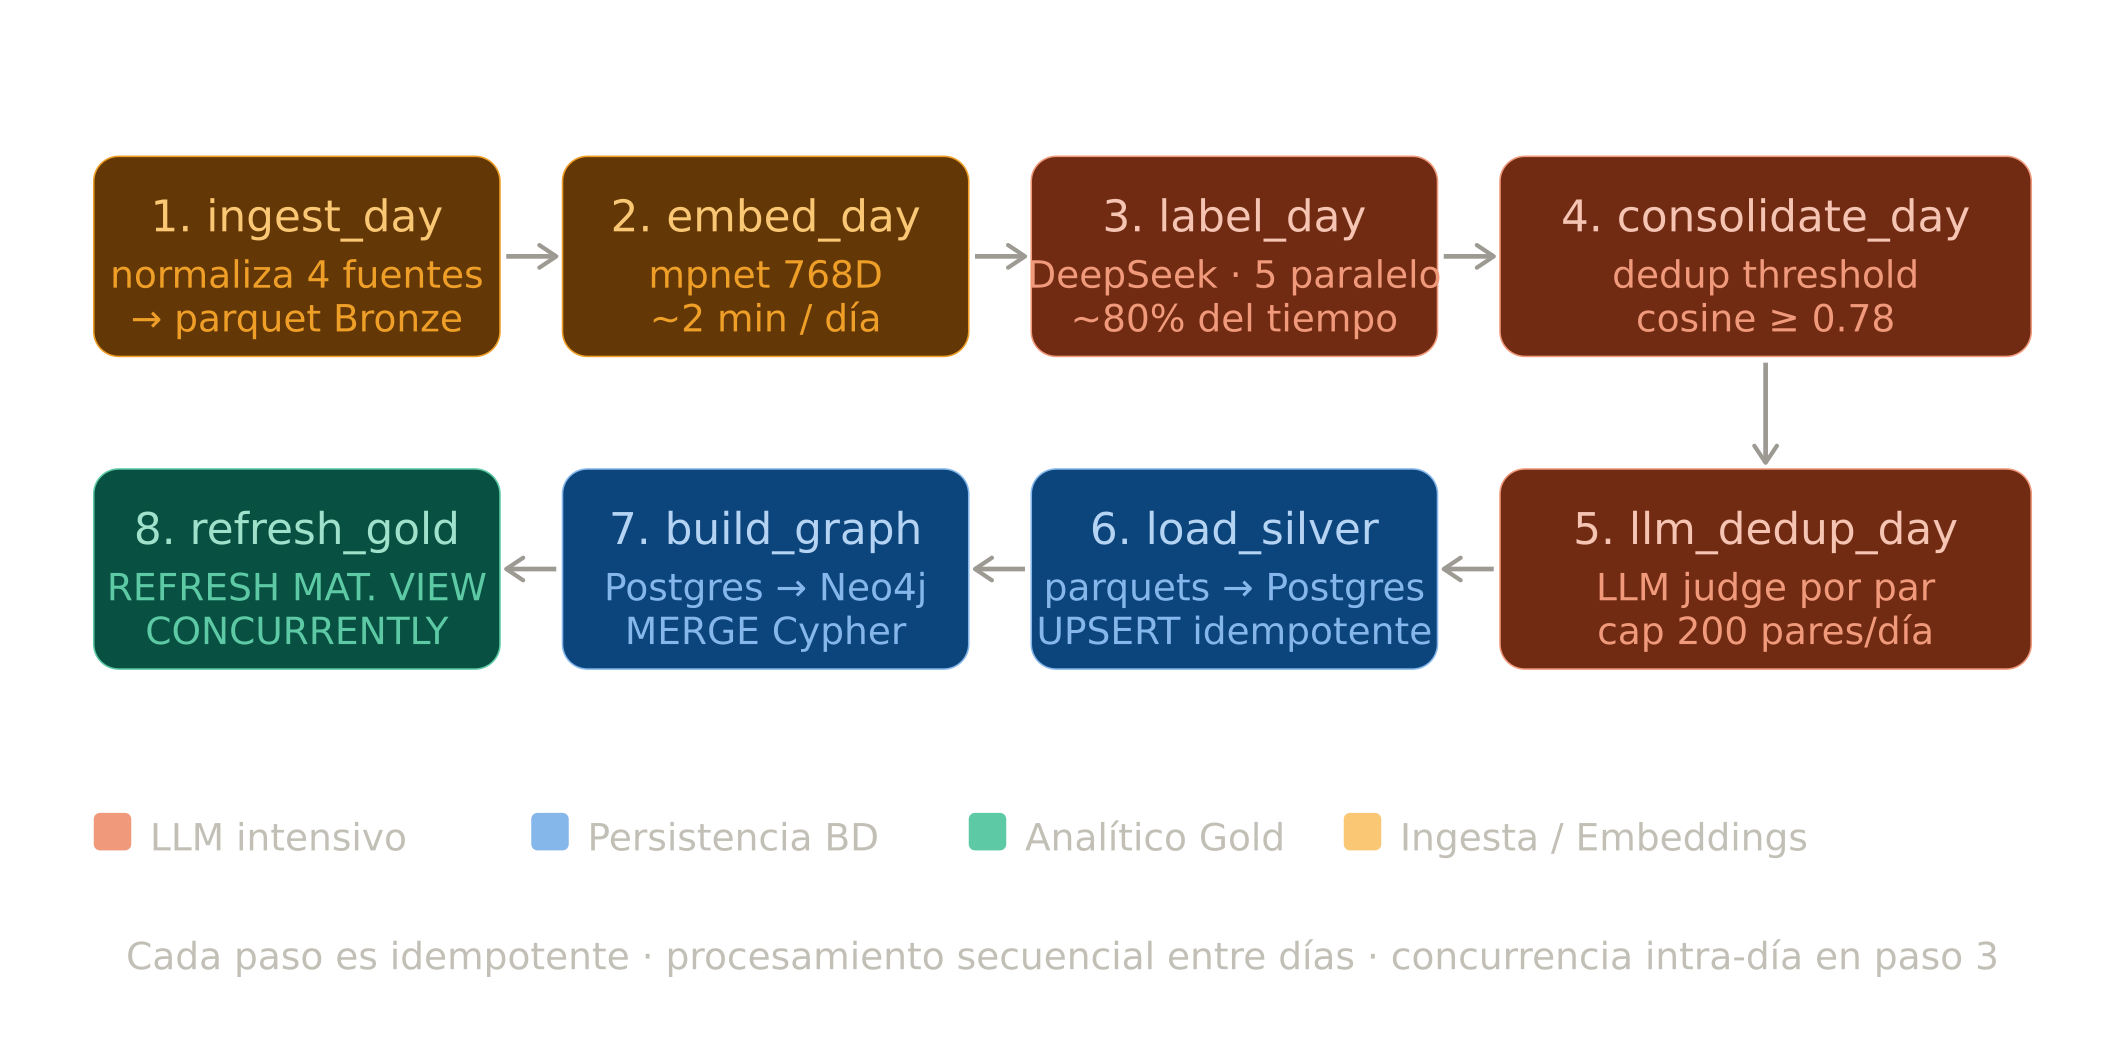
\includegraphics[width=0.95\textwidth]{images/pipeline_8_pasos.png}
        \caption[Pipeline completo del sistema de inteligencia electoral]{Pipeline completo del sistema de inteligencia electoral implementado: recolección multi-fuente, almacenamiento Bronze, normalización Silver, análisis LLM, deduplicación semántica, embeddings vectoriales, vistas Gold y exposición mediante MCP.\\
        Fuente: Elaboración propia.}
        \label{fig:real_pipeline_8steps}
    \end{center}
\end{figure}

\subsubsection{Medición de la Percepción Pública Nacional}
 
La \textbf{percepción pública nacional} en el contexto electoral se refiere al conjunto de actitudes, opiniones y emociones que los ciudadanos expresan colectivamente —en especial en ecosistemas digitales— hacia candidatos, partidos políticos, propuestas programáticas e instituciones democráticas. Su medición mediante LLMs ofrece ventajas sustanciales respecto a las encuestas tradicionales: es continua (no puntual), de bajo costo, capaz de procesar millones de expresiones ciudadanas simultáneamente y de detectar cambios bruscos de opinión asociados a eventos específicos de la campaña \parencite{pr_gujral2024llm_elections}.
 
Sin embargo, es importante reconocer sus limitaciones metodológicas: la representatividad del universo digital no es idéntica al electorado real, y los sesgos de los datos de entrenamiento de los LLMs pueden introducir distorsiones sistemáticas en las clasificaciones de sentimiento hacia ciertos actores políticos \parencite{pr_gujral2024llm_elections}. La triangulación con otras fuentes de datos y la interpretación crítica de los resultados son, por tanto, componentes indispensables de cualquier sistema de inteligencia electoral responsable.

% ──────────────────────────────────────────────────────────────
\subsection{Arquitectura Medallion para Pipelines de Datos}
% ──────────────────────────────────────────────────────────────

La arquitectura Medallion es un patrón de diseño para pipelines de procesamiento de datos que organiza la información en tres capas semánticas progresivas \parencite{bk_databricks2023medallion}.

La capa \textbf{Bronze} almacena los datos crudos tal como son ingeridos de las fuentes externas, sin transformación. La capa \textbf{Silver} contiene datos limpios, normalizados y enriquecidos, validados mediante esquemas formales. Finalmente, la capa \textbf{Gold} expone vistas analíticas materializadas, pre-agregadas para consultas de alto rendimiento.

Este patrón garantiza la reproducibilidad de cada etapa del pipeline: si un paso falla, puede reejecutarse desde el parquet de su capa de entrada sin re-invocar servicios externos costosos como las APIs de LLM.

La Figura \ref{fig:medallion_architecture} muestra la arquitectura Medallion aplicada al sistema de inteligencia electoral propuesto.

\begin{figure}[!ht]
    \begin{center}
        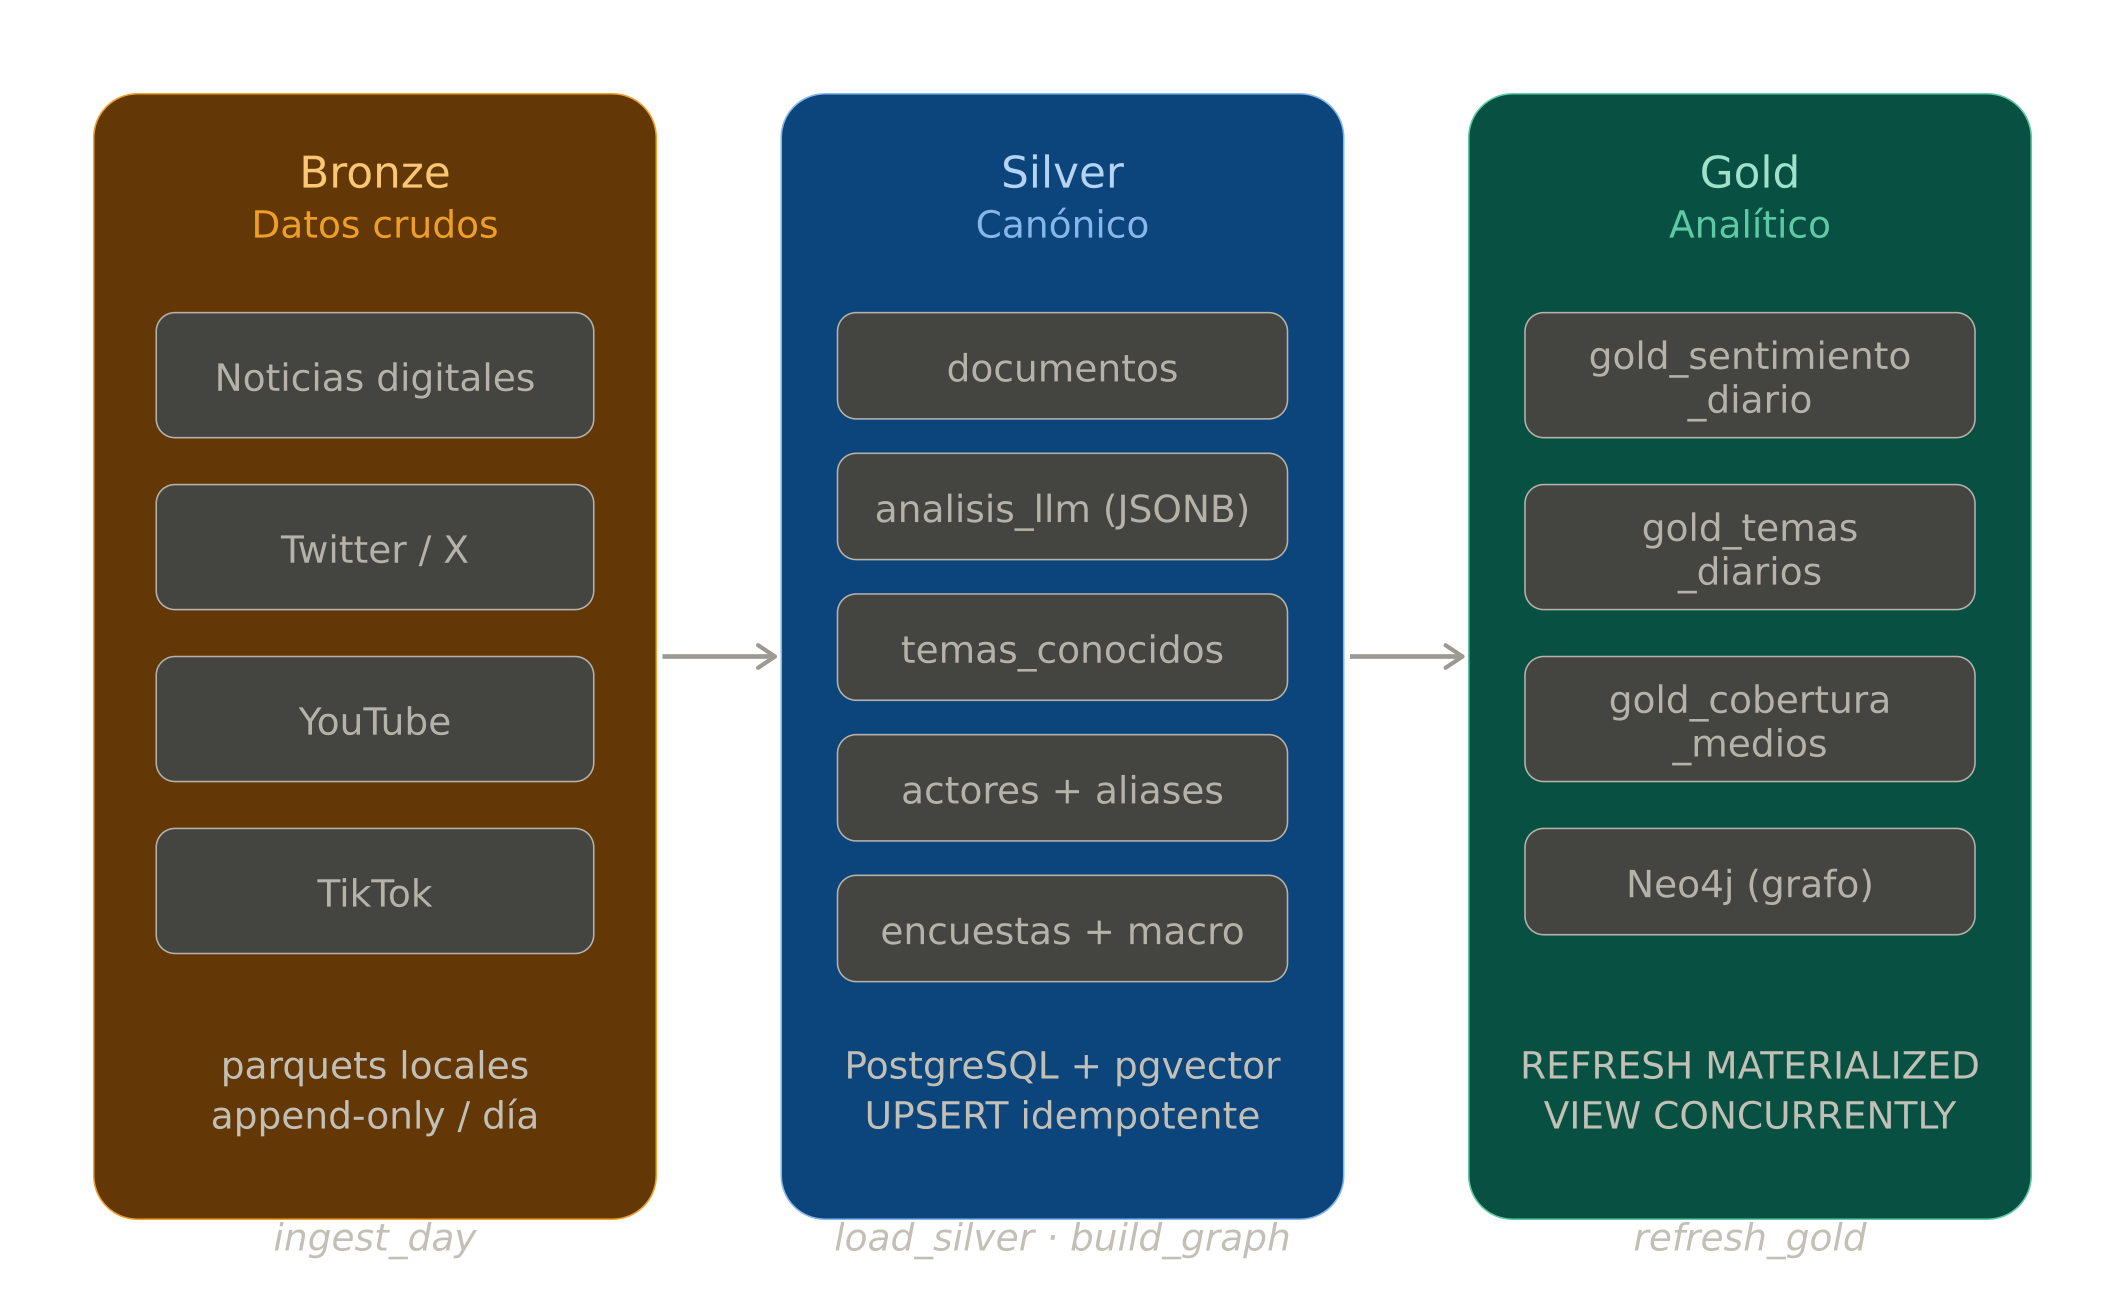
\includegraphics[width=0.92\textwidth]{images/medallion_architecture.png}
        \caption[Arquitectura Medallion del pipeline electoral]{Arquitectura Medallion del pipeline electoral: capa Bronze (datos crudos de 4 fuentes), capa Silver (documentos normalizados, análisis LLM, temas canónicos, actores) y capa Gold (vistas materializadas para análisis: sentimiento diario, temas diarios, cobertura de medios).\\
        Fuente: Elaboración propia.}
        \label{fig:medallion_architecture}
    \end{center}
\end{figure}

% ──────────────────────────────────────────────────────────────
\subsection{Bases de Datos Vectoriales y pgvector}
% ──────────────────────────────────────────────────────────────

Una base de datos vectorial es un sistema de almacenamiento especializado en la indexación y búsqueda eficiente de vectores de alta dimensión mediante métricas de similitud como la distancia coseno o euclidiana \parencite{tec_pan2024vectordb}.

La extensión \textbf{pgvector} integra estas capacidades directamente en PostgreSQL, permitiendo la creación de índices HNSW (\textit{Hierarchical Navigable Small World}) sobre columnas de tipo \texttt{vector(N)} y la ejecución de búsquedas de vecinos más cercanos mediante el operador \texttt{<=>} \parencite{tec_pgvector2024}.

Esta integración elimina la necesidad de mantener una base de datos vectorial dedicada (Pinecone, Weaviate, Qdrant), reduciendo la complejidad operacional y permitiendo combinar en una única query SQL la búsqueda semántica con filtros relacionales clásicos por fecha, fuente o candidato.

% ──────────────────────────────────────────────────────────────
\subsection{Model Context Protocol (MCP)}
% ──────────────────────────────────────────────────────────────

El Model Context Protocol (MCP) es un protocolo abierto propuesto por Anthropic en 2024 que estandariza la comunicación entre clientes de LLM (como Claude Desktop o Claude.ai) y servidores de herramientas externas \parencite{tec_anthropic2024mcp}.

El protocolo define un mecanismo de descubrimiento de herramientas (\textit{tools/list}), invocación tipada (\textit{tools/call}) y respuesta estructurada con validación de esquema JSON, permitiendo que un LLM consulte bases de datos, APIs y sistemas externos de forma estandarizada.

En el contexto de la inteligencia electoral, MCP permite exponer el grafo de conocimiento y las vistas analíticas Gold como herramientas invocables directamente desde una conversación con el LLM, sin necesidad de un dashboard separado.

% ──────────────────────────────────────────────────────────────
\subsection{Deduplicación Semántica de Entidades}
% ──────────────────────────────────────────────────────────────

La deduplicación semántica es el proceso de identificar y consolidar entidades que refieren al mismo concepto pero son expresadas con variaciones léxicas, ortográficas o de nivel de abstracción \parencite{tec_mudgal2018deepmatcher}.

En sistemas de análisis de discurso político, este problema se manifiesta cuando el LLM etiqueta el mismo suceso con denominaciones ligeramente distintas en documentos procesados en paralelo (por ejemplo, \textit{guerra\_estados\_unidos} y \textit{atentado\_inicio\_guerra}).

La deduplicación puede realizarse mediante:
\begin{enumerate}
    \item Comparación de similitud coseno entre embeddings de los temas.
    \item Coincidencia difusa de nombres mediante algoritmos como \textit{token set ratio} de la librería RapidFuzz.
    \item Juicio semántico de un LLM como árbitro final sobre pares sospechosos.
\end{enumerate}

La combinación de estos tres niveles, en un pipeline de tres etapas (dedup intra-batch, consolidación threshold-based y dedup LLM-judge), reduce la fragmentación del catálogo de temas sin introducir falsos positivos.



\section{Marco Conceptual}
% ──────────────────────────────────────────────────────────────
\subsection{Ecosistema Digital Electoral}
% ──────────────────────────────────────────────────────────────
 
El ecosistema digital electoral es el conjunto de plataformas, actores y flujos de información que operan en el entorno digital durante un proceso electoral, y a través del cual los ciudadanos expresan opiniones, debaten propuestas, comparten noticias y construyen o destruyen la imagen pública de los candidatos \parencite{mc_chadwick2013hybrid}. A diferencia de los medios tradicionales —prensa escrita, radio y televisión—, este ecosistema se caracteriza por la descentralización de la producción de contenido, la velocidad casi instantánea de difusión y la posibilidad de interacción directa entre ciudadanos y actores políticos.
 
El ecosistema digital electoral está compuesto por tres tipos de actores. Los \textbf{actores institucionales} incluyen partidos políticos, candidatos y organismos electorales que utilizan las plataformas digitales de manera estratégica para comunicar sus propuestas y movilizar votantes. Los \textbf{actores mediáticos digitales} son los medios de comunicación nativos digitales, blogs especializados y portales de noticias que cubren la campaña en tiempo real. Finalmente, los \textbf{ciudadanos} son quienes generan el mayor volumen de contenido a través de sus publicaciones, comentarios y reacciones en redes sociales, constituyendo la fuente primaria de datos para los sistemas de inteligencia electoral \parencite{mc_ceron2017social}.
 
La comprensión de este ecosistema es fundamental para la presente investigación, ya que los datos recolectados para el análisis de percepción pública nacional provienen de las interacciones que tienen lugar en él.
 
% ──────────────────────────────────────────────────────────────
\subsection{Percepción Pública}
% ──────────────────────────────────────────────────────────────
 
La percepción pública es el proceso cognitivo y evaluativo mediante el cual la ciudadanía forma juicios colectivos sobre personas, instituciones, eventos o políticas públicas, a partir de la información disponible en su entorno \parencite{mc_lippmann1922public}. En el contexto electoral, la percepción pública se manifiesta en las actitudes que los ciudadanos expresan hacia los candidatos, los partidos políticos, las propuestas programáticas y los resultados de gestión de los gobiernos.
 
Tradicionalmente, la percepción pública se medía mediante encuestas de opinión y grupos focales. Sin embargo, el auge de las redes sociales ha generado un flujo continuo y masivo de expresiones ciudadanas que constituyen un indicador alternativo —y complementario— de la percepción pública, con ventajas significativas: es ininterrumpido, de bajo costo, de alta escala y capaz de capturar cambios en tiempo real asociados a eventos específicos de la campaña \parencite{mc_ceron2017social}.
 
En el marco de esta investigación, la percepción pública nacional se operacionaliza como el conjunto de sentimientos, emociones y evaluaciones que los ciudadanos peruanos expresan en ecosistemas digitales en relación con el proceso electoral en curso, medidos a través de las técnicas de minería de sentimientos descritas en el presente trabajo.
 
% ──────────────────────────────────────────────────────────────
\subsection{Minería de Sentimientos}
% ──────────────────────────────────────────────────────────────
 
La minería de sentimientos, también conocida como análisis de sentimientos u opinión mining, es la disciplina del Procesamiento del Lenguaje Natural orientada a identificar, extraer y cuantificar automáticamente las actitudes subjetivas expresadas en textos digitales —sean estas positivas, negativas o neutras— hacia personas, entidades, productos, eventos o temas de interés \parencite{mc_liu2012sentiment}. Va más allá de la simple clasificación de polaridad al buscar identificar también la intensidad del sentimiento, la emoción subyacente y las entidades específicas hacia las que se dirigen dichas actitudes.
 
En el contexto de la inteligencia electoral, la minería de sentimientos permite responder preguntas como: ¿Qué proporción de la conversación digital expresa apoyo o rechazo hacia un candidato? ¿Cómo varía el sentimiento ciudadano antes y después de un debate presidencial? ¿Qué emociones predominan en la discusión sobre una propuesta de política pública? Las respuestas a estas preguntas ofrecen información valiosa y complementaria a las encuestas convencionales para la comprensión de la dinámica electoral \parencite{mc_ceron2017social}.
 
Formalmente, dado un conjunto de documentos $D = \{d_1, d_2, \ldots, d_n\}$, la minería de sentimientos busca asignar a cada documento $d_i$ una función de sentimiento $S(d_i, e_j) \in \{positivo, negativo, neutro\}$, donde $e_j$ representa una entidad o aspecto de interés (por ejemplo, un candidato político), como se representa en la Figura \ref{fig:sentiment_mining_process}.
 
\begin{figure}[!ht]
    \begin{center}
        
\includegraphics[width=0.85\textwidth]{images/sentiment_mining_process.jpg}
        \caption[Proceso general de la minería de sentimientos aplicada al análisis electoral]{Proceso general de la minería de sentimientos en el contexto electoral: desde la recolección de publicaciones hasta la generación de indicadores de percepción pública por candidato y tema.\\
            Fuente: Elaboración propia basada en \cite{mc_liu2012sentiment}.}
        \label{fig:sentiment_mining_process}
    \end{center}
\end{figure}
 
% ──────────────────────────────────────────────────────────────
\subsection{Tema Relevante}
% ──────────────────────────────────────────────────────────────
 
En el contexto de la presente investigación, un \textbf{tema relevante} (\textit{relevant topic}) se define como un conjunto coherente de términos, conceptos y narrativas que emergen de manera recurrente en la conversación digital sobre el proceso electoral, y que refleja una preocupación, debate o acontecimiento de interés colectivo para la ciudadanía \parencite{mc_blei2012lda}. La relevancia de un tema se determina por su frecuencia relativa en el corpus de publicaciones analizadas, su persistencia en el tiempo y su capacidad de articular distintas perspectivas ciudadanas.
 
Los temas relevantes en un ecosistema digital electoral pueden agruparse en varias categorías: temas programáticos (economía, salud, educación, seguridad), temas de imagen (honestidad, liderazgo, experiencia de los candidatos), temas contingentes (escándalos, revelaciones, hechos inesperados de la campaña) y temas sistémicos (confianza en las instituciones democráticas, participación ciudadana). La capacidad de identificar y monitorear estos temas de manera automática y en tiempo real es uno de los objetivos centrales de un sistema de inteligencia electoral basado en LLMs.
 
% ──────────────────────────────────────────────────────────────
\subsection{Detección Dinámica de Temas}
% ──────────────────────────────────────────────────────────────
 
La detección dinámica de temas es la capacidad de un sistema computacional para identificar automáticamente los temas latentes presentes en un corpus de textos y rastrear su evolución a lo largo del tiempo, sin requerir etiquetado manual previo ni un conjunto predefinido de categorías temáticas \parencite{mc_grootendorst2022bertopic}. El adjetivo «dinámica» hace referencia a que el sistema es capaz de detectar no solo los temas que ya existían al inicio del período de análisis, sino también los que emergen durante el proceso como respuesta a nuevos eventos, los que se intensifican y los que decaen.
 
En el contexto electoral, la detección dinámica de temas responde a preguntas como: ¿Qué nuevos asuntos han irrumpido en la conversación digital esta semana? ¿Cuáles han perdido relevancia? ¿Existe una correlación entre la aparición de un tema y un evento específico de la campaña? Este tipo de análisis es imposible de realizar manualmente a la escala de datos generados por las redes sociales durante un proceso electoral, de ahí la necesidad de automatizarlo mediante LLMs y modelos de topic modeling como BERTopic \parencite{mc_grootendorst2022bertopic}.
 
La Figura \ref{fig:dynamic_detection_concept} ilustra el concepto de detección dinámica de temas en el contexto electoral, mostrando cómo distintos temas emergen, se intensifican y decaen a lo largo del tiempo en respuesta a los hitos de la campaña.
 
\begin{figure}[!ht]
    \begin{center}
        \includegraphics[width=0.88\textwidth]{images/dynamic_detection_concept.jpg}
        \caption[Concepto de detección dinámica de temas en un proceso electoral]{Representación conceptual de la detección dinámica de temas en un proceso electoral: los temas emergen y decaen en función de los hitos de campaña (debates, anuncios, escándalos), siendo identificados automáticamente por el sistema.\\
            Fuente: Elaboración propia.}
        \label{fig:dynamic_detection_concept}
    \end{center}
\end{figure}
 
% ──────────────────────────────────────────────────────────────
\subsection{Corpus}
% ──────────────────────────────────────────────────────────────
 
En lingüística computacional y NLP, un \textbf{corpus} (plural: \textit{corpora}) es una colección estructurada y representativa de textos en formato digital, recopilados con un propósito analítico específico y que sirven como base de datos para el entrenamiento, ajuste fino o evaluación de modelos de procesamiento del lenguaje \parencite{mc_manning1999foundations}. La calidad, representatividad y tamaño del corpus son factores determinantes en la calidad de los análisis de sentimientos y detección de temas que se puedan derivar de él.
 
Para la presente investigación, el corpus está constituido por publicaciones extraídas de plataformas de redes sociales —principalmente X (antes Twitter)— relacionadas con el proceso electoral peruano, recolectadas mediante palabras clave, hashtags y cuentas de usuarios relevantes. Las características de este corpus —su tamaño, composición temporal, distribución de temas y balance entre clases de sentimiento— son descritas en detalle en el capítulo metodológico.
 
% ──────────────────────────────────────────────────────────────
\subsection{Token y Tokenización}
% ──────────────────────────────────────────────────────────────
 
Un \textbf{token} es la unidad mínima de procesamiento en la que se divide un texto para ser procesado por un modelo de NLP o un LLM. Dependiendo del tokenizador utilizado, un token puede corresponder a una palabra completa, a un subconjunto de caracteres de una palabra (\textit{subword}), a un signo de puntuación o incluso a un espacio en blanco \parencite{mc_devlin2018bert}. Los LLMs modernos utilizan tokenizadores de subpalabras como BPE (\textit{Byte Pair Encoding}) o WordPiece, que permiten manejar vocabularios abiertos y palabras fuera del vocabulario de entrenamiento.
 
La \textbf{tokenización} es el proceso de segmentar un texto de entrada en tokens antes de su procesamiento por el modelo, como se ilustra en la Figura \ref{fig:tokenization_example}. Este proceso es un paso previo indispensable en cualquier pipeline de NLP y tiene implicaciones directas en el rendimiento del modelo: textos en español político, con sus variantes léxicas regionales y uso de jerga electoral, presentan desafíos particulares de tokenización que deben ser considerados en el diseño del sistema.
 
\begin{figure}[!ht]
    \begin{center}
        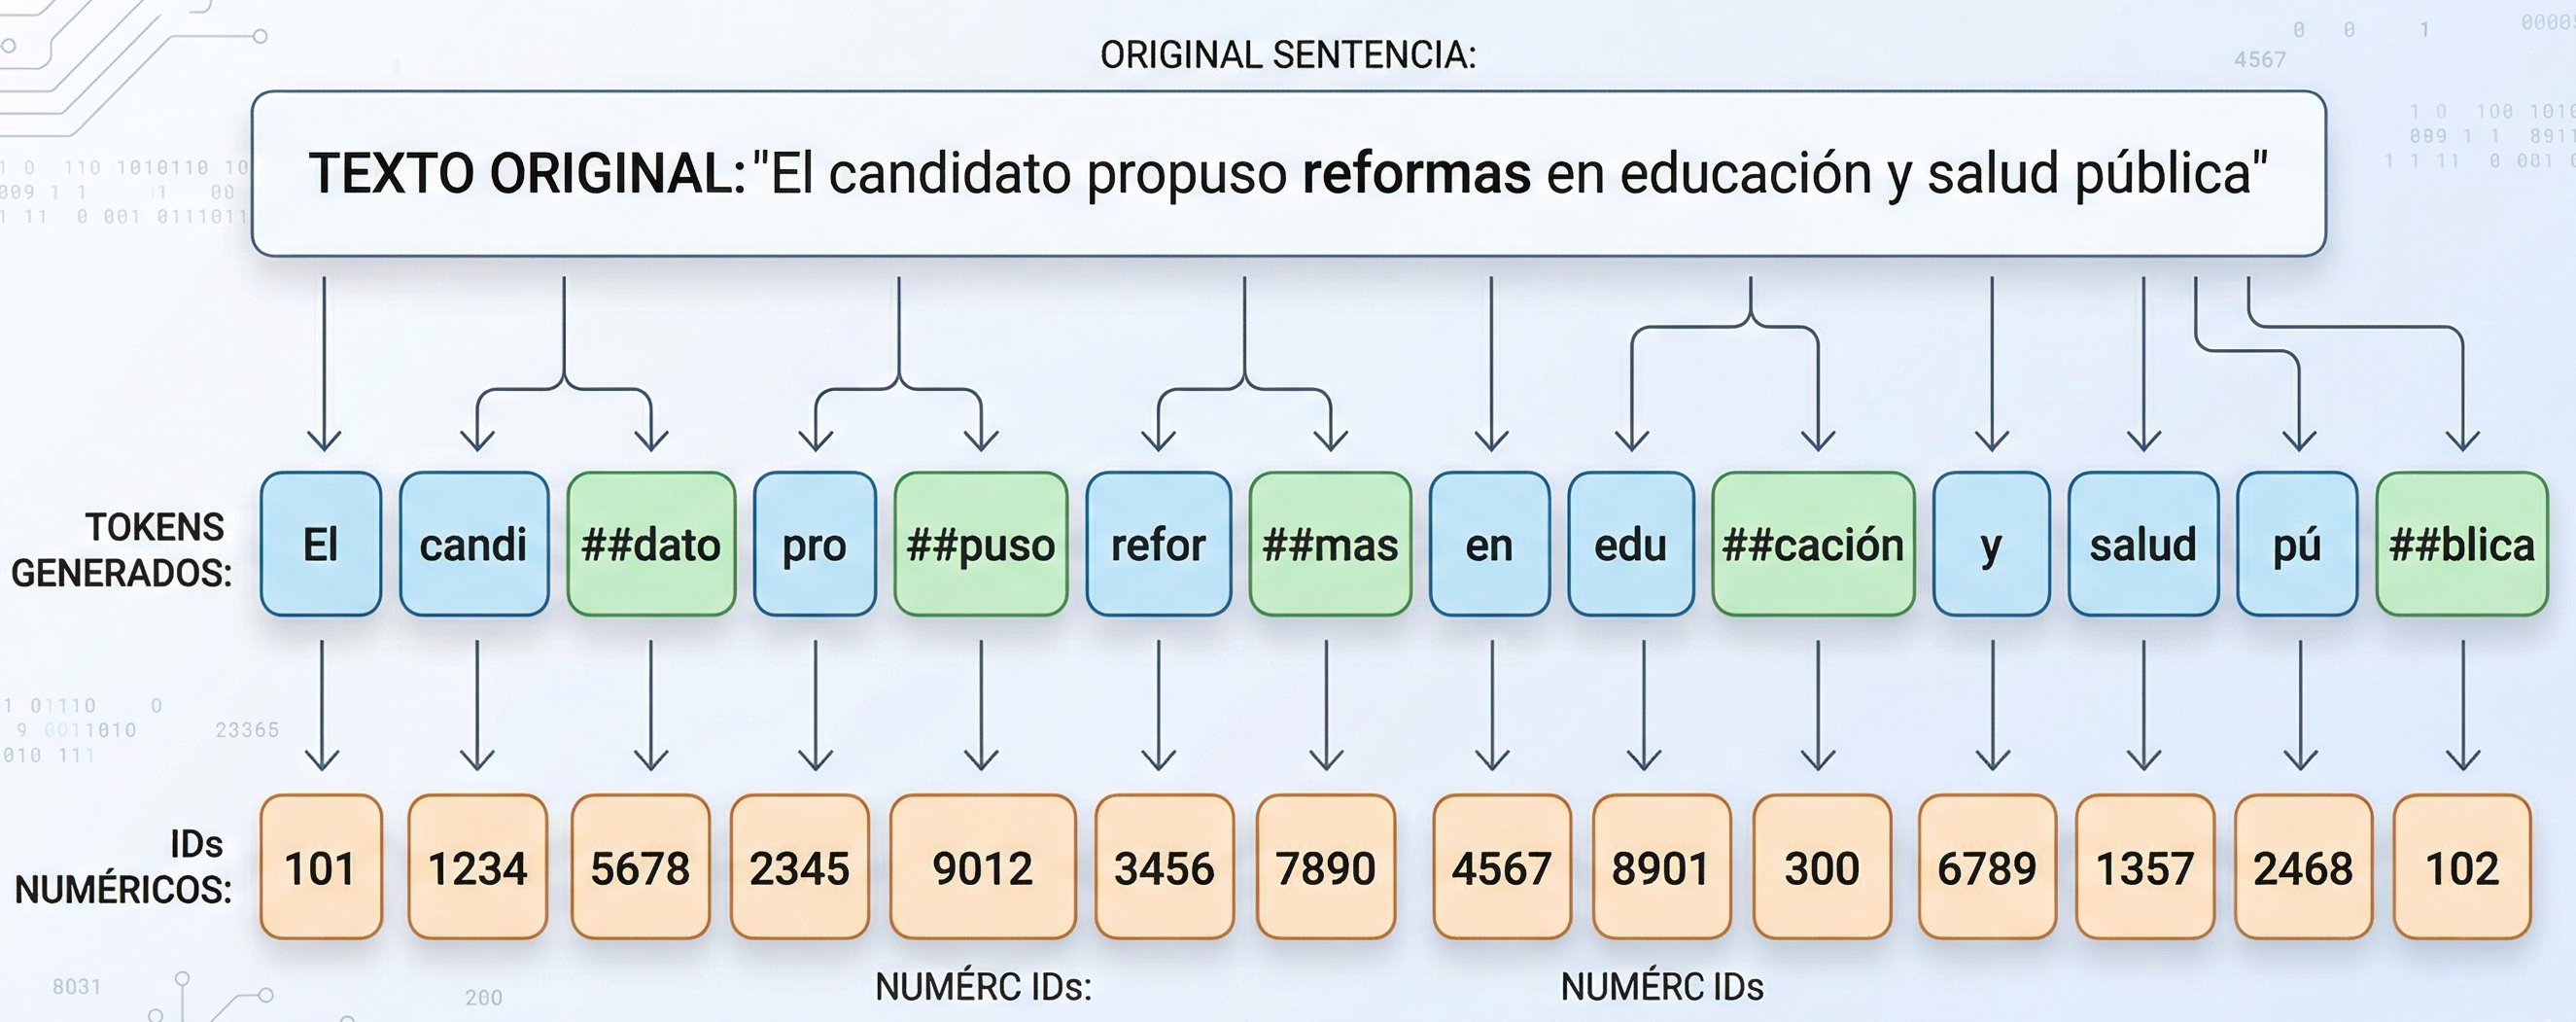
\includegraphics[width=0.82\textwidth]{images/tokenization_example.jpg}
        \caption[Ejemplo de tokenización de un texto político con tokenizadores de subpalabras]{Ejemplo de tokenización BPE aplicada a un texto político en español: la oración es dividida en tokens de subpalabras que el LLM puede procesar como vectores numéricos.\\
            Fuente: Elaboración propia basada en \cite{mc_devlin2018bert}.}
        \label{fig:tokenization_example}
    \end{center}
\end{figure}
 
% ──────────────────────────────────────────────────────────────
\subsection{Embedding o Incrustación Semántica}
% ──────────────────────────────────────────────────────────────
 
Un \textbf{embedding} (o incrustación semántica) es una representación vectorial densa de un token, palabra, oración o documento en un espacio de alta dimensión, donde la proximidad geométrica entre dos vectores refleja la similitud semántica entre los elementos que representan \parencite{mc_mikolov2013word2vec}. A diferencia de las representaciones dispersas como la Bolsa de Palabras o la codificación en caliente, los embeddings capturan relaciones semánticas y sintácticas complejas en un espacio de dimensión reducida.
 
En el contexto de la presente investigación, los embeddings cumplen dos roles fundamentales. Por un lado, los \textbf{embeddings de palabras} generados por modelos como Word2Vec o GloVe permiten calcular la similitud semántica entre términos políticos y construir representaciones del vocabulario electoral. Por otro lado, los \textbf{embeddings de oraciones} generados por modelos como Sentence-BERT \parencite{mc_reimers2019sbert} constituyen la entrada al pipeline de BERTopic para la detección dinámica de temas, ya que capturan el significado global de cada publicación en un único vector denso, como se representa en la Figura \ref{fig:embedding_space}.
 
\begin{figure}[!ht]
    \begin{center}
        \includegraphics[width=0.80\textwidth]{images/embedding_space.jpg}
        \caption[Espacio vectorial de embeddings de oraciones sobre discurso político electoral]{Representación del espacio vectorial de embeddings de oraciones políticas: publicaciones semánticamente similares se agrupan en regiones próximas del espacio, facilitando la posterior detección de temas mediante clustering.\\
            Fuente: Elaboración propia basada en \cite{mc_reimers2019sbert}.}
        \label{fig:embedding_space}
    \end{center}
\end{figure}
 
% ──────────────────────────────────────────────────────────────
\subsection{Prompt}
% ──────────────────────────────────────────────────────────────
 
Un \textbf{prompt} es la instrucción textual o consulta que se proporciona como entrada a un LLM para orientar y condicionar la respuesta que este genera \parencite{mc_white2023prompt}. El diseño del prompt es el mecanismo principal a través del cual el usuario comunica al modelo la tarea que debe realizar, el contexto en el que debe operar, el formato de la respuesta esperada y las restricciones que debe respetar, todo ello sin modificar los parámetros internos del modelo.
 
En el contexto de la inteligencia electoral, los prompts se utilizan para instrucciones como: «Clasifica el sentimiento de la siguiente publicación hacia el candidato X como positivo, negativo o neutro y explica brevemente tu razonamiento», o «Identifica el tema principal de las siguientes publicaciones y etiquétalo con una frase descriptiva de no más de cinco palabras». La calidad del prompt determina directamente la calidad de los resultados del sistema, razón por la cual la ingeniería de prompts es una componente técnica central de la presente investigación.
 
Los elementos clave de un prompt bien diseñado para análisis electoral incluyen: (1) la definición del \textbf{rol} del modelo («Eres un analista político experto en discurso electoral latinoamericano»), (2) el \textbf{contexto} de la tarea (el proceso electoral analizado, el idioma, las entidades relevantes), (3) la \textbf{instrucción} específica (qué debe hacer el modelo con el texto de entrada), (4) el \textbf{formato} de la respuesta esperada (JSON estructurado, categoría única, texto libre), y (5) los \textbf{ejemplos} en modalidad few-shot cuando sea necesario, como se ilustra en la Figura \ref{fig:prompt_structure}.
 
\begin{figure}[!ht]
    \begin{center}
        
\includegraphics[width=0.85\textwidth]{images/prompt_structure.jpg}
        \caption[Estructura de un prompt optimizado para análisis de sentimientos electorales]{Estructura de un prompt bien diseñado para análisis de sentimientos electorales, mostrando sus cinco componentes: rol, contexto, instrucción, formato y ejemplos few-shot.\\
            Fuente: Elaboración propia basada en \cite{mc_white2023prompt}.}
        \label{fig:prompt_structure}
    \end{center}
\end{figure}
 
% ──────────────────────────────────────────────────────────────
\subsection{Polaridad}
% ──────────────────────────────────────────────────────────────
 
La \textbf{polaridad} es la dimensión evaluativa fundamental del análisis de sentimientos, que indica la orientación afectiva de un texto hacia una entidad o aspecto determinado: positiva, negativa o neutral \parencite{mc_liu2012sentiment}. En el contexto electoral, la polaridad mide si una publicación expresa apoyo, rechazo o una posición indefinida respecto a un candidato, partido político, propuesta o evento de la campaña.
 
Más allá de la clasificación ternaria básica (positivo / negativo / neutral), existen modelos de polaridad más granulares que incluyen escalas de intensidad —muy positivo, positivo, neutral, negativo, muy negativo— o que descomponen la polaridad en sus dimensiones emocionales constituyentes (alegría, enojo, miedo, sorpresa, tristeza, asco) siguiendo modelos como el de Plutchik \parencite{mc_plutchik1980emotion}. Los LLMs modernos son capaces de operar en este nivel de granularidad emocional, lo que constituye una ventaja significativa respecto a los clasificadores binarios clásicos.
 
En el presente trabajo, la polaridad se mide a nivel de aspecto (\textit{Aspect-Based Sentiment Analysis}), es decir, desagregada por entidad política: una misma publicación puede expresar polaridad positiva hacia una propuesta económica y negativa hacia la gestión en seguridad de un mismo candidato, capturando así la complejidad real del discurso político ciudadano.
 
% ──────────────────────────────────────────────────────────────
\subsection{Desinformación Electoral}
% ──────────────────────────────────────────────────────────────
 
La \textbf{desinformación electoral} es la producción y difusión deliberada de contenido falso, engañoso o manipulado con el propósito de distorsionar la percepción pública sobre candidatos, procesos electorales o resultados, con el fin de influir en el comportamiento de los votantes o deslegitimar las instituciones democráticas \parencite{mc_wardle2017information}. Se distingue de la \textbf{desinformación involuntaria} (\textit{misinformation}), que corresponde a la difusión de contenido falso sin intención de engañar.
 
En el ecosistema digital, la desinformación electoral puede adoptar múltiples formas: noticias falsas fabricadas (\textit{fake news}), imágenes o videos manipulados (\textit{deepfakes}), cuentas automatizadas (\textit{bots}) que amplifican artificialmente narrativas, o titulares descontextualizados que distorsionan hechos reales \parencite{pr_chen2024combating_misinformation}. La irrupción de los LLMs ha agravado este problema al facilitar la generación masiva de texto de apariencia creíble, aunque también ha abierto nuevas posibilidades para su detección automatizada mediante los mismos modelos.
 
En el sistema de inteligencia electoral propuesto en esta investigación, la detección de desinformación opera como un módulo complementario al análisis de sentimientos y la detección de temas, con el objetivo de garantizar que los indicadores de percepción pública no sean distorsionados por contenido falso amplificado artificialmente.
 
% ──────────────────────────────────────────────────────────────
\subsection{Polarización Política Digital}
% ──────────────────────────────────────────────────────────────
 
La \textbf{polarización política digital} es el fenómeno por el cual las conversaciones en ecosistemas digitales tienden a organizarse en dos o más grupos ideológicamente distantes, con escasa interacción entre ellos y con una progresiva intensificación del discurso afectivo negativo hacia el grupo contrario \parencite{mc_iyengar2019origins}. Este fenómeno, que en la literatura anglosajona se denomina también \textit{affective polarization} (polarización afectiva), es amplificado por los algoritmos de recomendación de las plataformas digitales, que tienden a reforzar las preferencias existentes de los usuarios en lugar de exponerlos a perspectivas diversas.
 
En el contexto de la inteligencia electoral, la medición de la polarización política digital es un indicador relevante de la salud del ecosistema de debate público: niveles extremos de polarización se asocian con mayor susceptibilidad a la desinformación, menor disposición al diálogo ciudadano y mayor volatilidad del comportamiento electoral \parencite{mc_iyengar2019origins}. Los LLMs permiten cuantificar la polarización a través del análisis de la distribución y la intensidad del sentimiento negativo entre grupos de usuarios y del monitoreo de las narrativas que cada grupo construye sobre el otro.
 
% ──────────────────────────────────────────────────────────────
\subsection{Monitoreo en Tiempo Real}
% ──────────────────────────────────────────────────────────────
 
El \textbf{monitoreo en tiempo real} (\textit{real-time monitoring}) es la capacidad de un sistema computacional para ingerir, procesar y analizar flujos continuos de datos digitales con una latencia mínima, generando resultados actualizados de manera casi instantánea \parencite{mc_garcia2025real_time}. En el contexto de la inteligencia electoral, esto significa que el sistema es capaz de detectar un cambio brusco en el sentimiento ciudadano o la emergencia de un nuevo tema en el ecosistema digital en cuestión de minutos desde que el evento desencadenante ocurre, permitiendo a los analistas políticos y periodistas actuar sobre información actualizada.
 
El monitoreo en tiempo real requiere una arquitectura de software específica que incluye: (1) un módulo de ingesta de datos en streaming (por ejemplo, mediante la API de X/Twitter Filtered Stream), (2) un módulo de preprocesamiento que limpia y normaliza el texto a medida que llega, (3) un módulo de inferencia con el LLM que clasifica sentimientos y detecta temas de manera paralela, y (4) un módulo de visualización que actualiza los dashboards en tiempo real con los nuevos resultados, como se esquematiza en la Figura \ref{fig:realtime_architecture}.
 
\begin{figure}[!ht]
    \begin{center}
        
\includegraphics[width=0.90\textwidth]{images/realtime_architecture.jpg}
        \caption[Arquitectura de procesamiento en tiempo real para monitoreo de percepción electoral]{Arquitectura de un sistema de monitoreo electoral en tiempo real: ingesta de datos en streaming, preprocesamiento, inferencia LLM paralela y actualización de dashboards de visualización.\\
            Fuente: Elaboración propia basada en \cite{mc_garcia2025real_time}.}
        \label{fig:realtime_architecture}
    \end{center}
\end{figure}
 
% ──────────────────────────────────────────────────────────────
\subsection{Indicadores de Percepción Electoral}
% ──────────────────────────────────────────────────────────────
 
Los \textbf{indicadores de percepción electoral} son métricas cuantitativas derivadas del análisis de datos del ecosistema digital que permiten operacionalizar y medir de manera sistemática la percepción pública hacia candidatos, partidos, temas y el proceso electoral en general \parencite{mc_ceron2017social}. En la presente investigación se definen los siguientes indicadores principales:
 
El \textbf{Índice de Sentimiento Neto} (ISN) mide la diferencia entre la proporción de publicaciones con sentimiento positivo y negativo hacia una entidad política en un período determinado, calculado mediante la Ecuación \ref{eq:isn}:
 
\begin{equation}\label{eq:isn}
\phantomsection
ISN_{(e,t)} = \frac{P_{pos}(e,t) - P_{neg}(e,t)}{P_{total}(e,t)} \times 100
\end{equation}
\myequations{Índice de Sentimiento Neto para entidades políticas}
 
Donde:
\begin{conditions}
P_{pos}(e,t)    & número de publicaciones con sentimiento positivo hacia la entidad $e$ en el período $t$ \\
P_{neg}(e,t)    & número de publicaciones con sentimiento negativo hacia la entidad $e$ en el período $t$ \\
P_{total}(e,t)  & número total de publicaciones que mencionan a la entidad $e$ en el período $t$
\end{conditions}
 
El \textbf{Índice de Relevancia Temática} (IRT) mide la importancia relativa de un tema en el corpus en un período dado, calculado como la proporción de publicaciones asignadas a ese tema sobre el total del corpus en ese período. El \textbf{Índice de Velocidad de Emergencia} (IVE) mide la rapidez con la que un tema nuevo gana relevancia, calculado como la derivada temporal del IRT. Estos tres indicadores, monitoreados conjuntamente en tiempo real, constituyen el núcleo analítico del sistema de inteligencia electoral propuesto.

\chapter{Entorno Empresarial}
 
\section{Descripción del contexto de aplicación}
 
\subsection{Reseña histórica y actividad}
 
El Jurado Nacional de Elecciones (JNE) es el organismo constitucional autónomo del
Estado peruano encargado de administrar justicia en materia electoral, fiscalizar la
legalidad del ejercicio del sufragio y de la realización de los procesos electorales, de
referéndum y de otras consultas populares Jurado Nacional de Elecciones (2023). Fue creado
mediante la Constitución Política de 1933 y reafirmado como organismo autónomo por la
Constitución vigente de 1993, siendo hoy uno de los tres organismos electorales del
sistema democrático peruano, junto a la Oficina Nacional de Procesos Electorales (ONPE)
y el Registro Nacional de Identificación y Estado Civil (RENIEC).
 
En el marco de los procesos electorales, la percepción pública de la ciudadanía hacia
los candidatos, partidos políticos y propuestas programáticas se construye y transforma
principalmente en el ecosistema digital. Las redes sociales —en especial X (antes Twitter),
Facebook y TikTok— se han consolidado como las principales arenas de debate político
nacional durante las campañas electorales peruanas de 2021, 2022 y 2026. Sin embargo,
el análisis sistemático y en tiempo real de este flujo de información ha sido hasta la fecha
un reto técnico sin resolver a escala institucional.
 
La presente investigación se desarrolla como un proyecto académico aplicado orientado al análisis automatizado de percepción pública electoral en ecosistemas digitales peruanos. Para ello, se trabaja con un equipo multidisciplinario conformado por analistas políticos, especialistas en NLP e ingenieros de datos, cuyo interés es evaluar la viabilidad de un sistema automatizado de inteligencia electoral basado en Modelos de Lenguaje de Gran Escala (LLMs).
 
\subsection{Descripción de la organización}
 
\subsubsection{Organigrama del equipo de investigación aplicada}
 
El equipo de trabajo vinculado al desarrollo e implementación del sistema de
inteligencia electoral propuesto en esta tesis está conformado por los siguientes roles, cuya
estructura jerárquica se representa en la Figura \ref{fig:organigrama_equipo}.
 
\begin{itemize}
    \item \textbf{Director del Proyecto}: Responsable de la visión estratégica, la
    definición de los objetivos del sistema y la validación de los resultados desde una
    perspectiva de ciencia política. Coordina con los organismos electorales y los medios
    de comunicación interesados en el producto final.
 
    \item \textbf{Líder de Ciencia de Datos / NLP}: Diseña la arquitectura del pipeline de
    procesamiento de lenguaje natural, selecciona y ajusta los modelos LLM utilizados, y
    supervisa la calidad de los análisis de sentimientos y detección de temas.
 
    \item \textbf{Ingeniero de Datos}: Responsable de la ingesta, almacenamiento y
    preprocesamiento de los datos de redes sociales en tiempo real. Gestiona las
    conexiones con las APIs de las plataformas digitales y los sistemas de base de datos.
 
    \item \textbf{Analista Político Electoral}: Experto en el contexto político peruano que
    valida cualitativamente los resultados del sistema, define los criterios de relevancia
    temática y asegura que los indicadores generados sean interpretables y útiles para la
    toma de decisiones.
 
    \item \textbf{Desarrollador de Visualización}: Diseña e implementa los dashboards
    interactivos que permiten explorar los resultados del sistema en tiempo real, así como
    los reportes automáticos generados al cierre de cada jornada electoral.
 
    \item \textbf{Especialista en Ética e Integridad Electoral}: Supervisa que el sistema
    opere dentro de los marcos legales y éticos aplicables, previene el uso indebido de los
    resultados y asegura la privacidad y anonimización de los datos ciudadanos
    procesados.
\end{itemize}
 
\begin{figure}[!ht]
    \begin{center}
        \includegraphics[width=0.82\textwidth]{images/organigrama_equipo.jpg}
        \caption[Organigrama del equipo de investigación del sistema de inteligencia electoral]{Organigrama del equipo de investigación y desarrollo del sistema de inteligencia electoral basado en LLMs, mostrando la jerarquía y relaciones entre los roles definidos.\\
            Fuente: Elaboración propia.}
        \label{fig:organigrama_equipo}
    \end{center}
\end{figure}
 
\subsubsection{Ecosistema de datos y fuentes de información}
 
El sistema de inteligencia electoral opera sobre un ecosistema de datos compuesto por
múltiples fuentes de información digital, cuya interacción y flujo se describen en la
Tabla \ref{tab:fuentes_datos}.
 
\begin{table}[htbp]
    \renewcommand\arraystretch{1.3} % Aumentamos un poco el espacio entre filas para mejor lectura
    \caption[Fuentes de datos del sistema de inteligencia electoral]{Fuentes de datos utilizadas por el sistema de inteligencia electoral y su rol dentro del pipeline analítico.}
    \label{tab:fuentes_datos}
    \centering
    \small % Cambiado de footnotesize a small para mantener consistencia con tus otras tablas
    \begin{tabular}{p{2.8cm} p{3.2cm} p{4.2cm} p{4.5cm}}
        \specialrule{.1em}{.05em}{.05em}
        \textbf{Fuente} & \textbf{Tipo de dato} & \textbf{Método de acceso} & \textbf{\arraybackslash Rol en el sistema} \\
        \specialrule{.1em}{.05em}{.05em}

        Noticias digitales &
        Artículos y titulares &
        Scrapers aiohttp + BeautifulSoup (8 medios) &
        Fuente primaria de análisis de sentimientos \\ 

        \hline

        Twitter / X &
        Tweets, retweets, menciones &
        TwitterAPI.io (REST, tercero) &
        Fuente primaria de sentimiento ciudadano \\ 

        \hline

        YouTube &
        Transcripciones y metadata &
        yt-dlp (web scraping) &
        Fuente de contenido audiovisual político \\ 

        \hline

        TikTok &
        Posts y metadata &
        yt-dlp (web scraping) &
        Fuente complementaria de alcance joven \\ 

        \hline

        Encuestas Datum &
        Intención de voto por candidato &
        JSON curado manualmente &
        Validación y calibración del sistema \\ 

        \hline

        BCRP &
        Tipo de cambio, IGBVL, EMBI &
        XLSX descargados (BCRP) &
        Contexto macroeconómico correlacional \\

        \specialrule{.1em}{.05em}{.05em}
    \end{tabular}

    \begin{flushleft}
        \small Fuente: Elaboración propia.
    \end{flushleft}
\end{table}
 
\section{Datos generales estratégicos}
 
\subsection{Visión, misión y objetivos del sistema}
 
\subsubsection{Visión del sistema}
 
«Ser el sistema de referencia en inteligencia electoral para el Perú, reconocido por
la precisión, transparencia y utilidad de sus análisis de percepción pública nacional
en ecosistemas digitales durante procesos electorales.»
 
\subsubsection{Misión del sistema}
 
«Proveer a analistas políticos, periodistas, organismos electorales e investigadores
académicos una plataforma automatizada de análisis de sentimientos y detección
dinámica de temas, basada en Modelos de Lenguaje de Gran Escala, que permita
comprender en tiempo real la percepción ciudadana nacional durante las campañas
electorales peruanas.»
 
\subsubsection{Valores y principios de diseño}
 
El sistema se rige por los siguientes principios fundamentales:
 
\begin{itemize}
    \item \textbf{Transparencia algorítmica}: Los criterios de clasificación de sentimientos y
    detección de temas son documentados y auditables, permitiendo la trazabilidad de los
    resultados generados por el LLM.
 
    \item \textbf{Neutralidad política}: El sistema no está diseñado para favorecer ni
    perjudicar a ningún candidato o partido político. Sus resultados reflejan la distribución
    real del sentimiento ciudadano en el ecosistema digital analizado.
 
    \item \textbf{Privacidad y anonimización}: Los datos individuales de los usuarios no son
    almacenados ni utilizados para fines distintos al análisis agregado. Se cumple con la
    Ley N.° 29733 de Protección de Datos Personales del Perú.
 
    \item \textbf{Rigor científico}: Todos los resultados del sistema son sometidos a
    procesos de validación cuantitativa y cualitativa antes de su presentación pública.
 
    \item \textbf{Accesibilidad}: Los reportes e indicadores generados están diseñados para
    ser comprensibles tanto por especialistas técnicos como por periodistas, comunicadores
    y ciudadanos sin formación en ciencia de datos.
\end{itemize}
 
\subsection{Objetivos estratégicos del sistema}
 
El sistema de inteligencia electoral propuesto tiene como objetivos estratégicos los
siguientes:
 
En primer lugar, \textbf{desarrollar un pipeline automatizado de análisis de sentimientos}
aplicado al discurso político peruano en redes sociales, utilizando LLMs en modalidad
zero-shot y few-shot, capaz de clasificar la polaridad y emoción de publicaciones en
español con una exactitud superior al 85\% validada contra etiquetas humanas.
 
En segundo lugar, \textbf{implementar un sistema de detección dinámica de temas} basado
en BERTopic y embeddings de Sentence-BERT, capaz de identificar automáticamente los
temas relevantes emergentes en el ecosistema digital electoral y rastrear su evolución
temporal durante el período de campaña.
 
En tercer lugar, \textbf{construir un módulo de detección de desinformación electoral} que
identifique narrativas potencialmente falsas o engañosas circulando en el ecosistema
digital, complementando el análisis de sentimientos con una capa de verificación
automática basada en técnicas de RAG (\textit{Retrieval-Augmented Generation}).
 
Finalmente, \textbf{diseñar y desplegar un dashboard de visualización en tiempo real} que
permita a los usuarios explorar los indicadores de percepción pública nacional —Índice
de Sentimiento Neto, Índice de Relevancia Temática e Índice de Velocidad de
Emergencia— de manera interactiva y actualizada.
 
\subsection{Evaluación interna y externa. FODA}
 
Con el apoyo del equipo analista y la revisión del ecosistema de herramientas de
inteligencia electoral existentes, se elaboró el análisis FODA del sistema propuesto,
presentado en la Tabla \ref{tab:foda_cruzado}, identificando las estrategias posibles según
la combinación de factores internos y externos.
 
\begin{table}[htbp]
    \caption[FODA cruzado del sistema de inteligencia electoral basado en LLMs]{FODA cruzado del sistema de inteligencia electoral basado en LLMs.}
    \label{tab:foda_cruzado}
    \scriptsize
    \centering
    \begin{tabular}{M{2.2cm}M{4.5cm}M{4.5cm}}
        \specialrule{.1em}{.05em}{.05em}
        & \textbf{FORTALEZAS} & \textbf{DEBILIDADES} \\
        & F1: Uso de LLMs de última generación &
          D1: Alta demanda computacional \\
        & F2: Pipeline completamente automatizado &
          D2: Dependencia de APIs de terceros \\
        & F3: Análisis en tiempo real &
          D3: Sesgo potencial en datos de Twitter \\
        & F4: Multilingüismo (español regional) &
          D4: Escasez de datos etiquetados en español político peruano \\
        \specialrule{.1em}{.05em}{.05em}
        \textbf{OPORTUNIDADES} & \textbf{Estrategia FO} & \textbf{Estrategia DO} \\
        O1: Creciente digitalización del debate político peruano &
        Aprovechar los LLMs multilingües para capturar el español político
        regional y posicionarse como herramienta de referencia en
        inteligencia electoral nacional. &
        Mitigar el sesgo de datos mediante la incorporación de múltiples
        fuentes (Twitter, Facebook, noticias), reduciendo la dependencia
        de una sola plataforma. \\[3pt]
        O2: Apertura de APIs electorales (ONPE/JNE) &
        Integrar datos oficiales del JNE y ONPE para validar y enriquecer
        los indicadores de percepción pública generados por el sistema. &
        Utilizar datos de encuestas tradicionales como conjunto de
        etiquetado para reducir la escasez de datos supervisados en
        español político. \\[3pt]
        O3: Crecimiento del uso de redes sociales en campañas electorales &
        Escalar el sistema para monitorear simultáneamente múltiples
        plataformas digitales durante la campaña. &
        Desarrollar módulos de fine-tuning con datos locales peruanos para
        reducir el sesgo de modelos pre-entrenados en inglés. \\
        \specialrule{.1em}{.05em}{.05em}
        \textbf{AMENAZAS} & \textbf{Estrategia FA} & \textbf{Estrategia DA} \\
        A1: Restricciones de acceso a APIs de redes sociales &
        Diversificar las fuentes de datos incluyendo portales de noticias
        y scraping ético para reducir la vulnerabilidad ante cambios en
        las políticas de las APIs. &
        Implementar sistemas de caché y procesamiento diferido para
        mantener la operatividad ante interrupciones en el acceso a
        las APIs. \\[3pt]
        A2: Uso malicioso del sistema para manipulación política &
        Diseñar protocolos de uso responsable y publicar los resultados
        solo en formatos agregados que no permitan la identificación de
        usuarios individuales. &
        Establecer alianzas con organismos electorales y académicos para
        garantizar la supervisión ética del sistema y prevenir su
        instrumentalización política. \\[3pt]
        A3: Evolución rápida del lenguaje político y la jerga digital &
        Aprovechar la capacidad de aprendizaje continuo de los LLMs para
        actualizar los modelos con nueva terminología política emergente. &
        Implementar ciclos periódicos de re-entrenamiento del modelo con
        datos actualizados para mantener la precisión ante la evolución del
        lenguaje político. \\
        \specialrule{.1em}{.05em}{.05em}
    \end{tabular}
    \begin{flushleft}
        \small Fuente: Elaboración propia.
    \end{flushleft}
\end{table}
 
En resumen, el sistema de inteligencia electoral propuesto se encuentra bien posicionado
para abordar una necesidad real e insatisfecha en el contexto electoral peruano. Sus
principales fortalezas —el uso de LLMs de última generación, la automatización del
pipeline y la capacidad de análisis en tiempo real— lo diferencian de los enfoques
convencionales de monitoreo político. A través de estrategias que combinan la integración
de datos oficiales, el desarrollo de capacidades multilingües en español regional y la
adhesión a principios éticos rigurosos, el sistema tiene la oportunidad de consolidarse como
una herramienta de referencia para analistas políticos, periodistas e investigadores durante
los procesos electorales peruanos.
 
\section{Modelo de negocio actual (CANVAS)}
 
El modelo de negocio del sistema de inteligencia electoral se estructura bajo el marco
Canvas, identificando sus componentes clave como se describe a continuación y se ilustra
en la Figura \ref{fig:canvas_sistema}.
 
\textbf{Propuesta de Valor}: Análisis automatizado de percepción pública electoral en
tiempo real; detección dinámica de temas relevantes emergentes en el ecosistema digital;
monitoreo de desinformación electoral; reportes de inteligencia política accionables para
la toma de decisiones en campaña.
 
\textbf{Segmentos de Clientes}: Equipos de campaña y partidos políticos; periodistas
y medios de comunicación digitales especializados en política; organismos electorales
(JNE, ONPE); investigadores académicos en ciencia política y comunicación; consultoras
de comunicación estratégica.
 
\textbf{Canales}: Plataforma web con dashboard interactivo en tiempo real; API de
resultados para integración con sistemas externos; reportes automatizados en PDF
enviados por correo electrónico; presentaciones de resultados en reuniones con clientes.
 
\textbf{Relaciones con Clientes}: Acceso a la plataforma mediante suscripción; soporte
técnico y capacitación en interpretación de resultados; reuniones periódicas de análisis
con los equipos usuarios; documentación técnica y metodológica detallada.
 
\textbf{Fuentes de Ingresos}: Suscripciones a la plataforma por período electoral;
contratos de análisis específico con organismos electorales; licenciamiento de la
metodología para centros de investigación académica; consultoría en comunicación
política basada en los resultados del sistema.
 
\textbf{Recursos Clave}: Modelos LLM pre-entrenados (DeepSeek, Llama, BERT multilingüe); infraestructura local basada en Docker Compose para procesamiento y almacenamiento; acceso a APIs y herramientas de scraping para redes sociales y medios digitales; base de datos PostgreSQL con pgvector; Neo4j Community Edition para almacenamiento del grafo de conocimiento; equipo multidisciplinario de científicos de datos, analistas políticos y desarrolladores.

\textbf{Actividades Clave}: Recolección y preprocesamiento de datos de redes sociales;
análisis de sentimientos con LLMs; detección dinámica de temas con BERTopic;
detección de desinformación; actualización y mantenimiento de los modelos; generación
de reportes e indicadores de percepción pública.
 
\textbf{Socios Clave}: Plataformas de redes sociales (proveedoras de APIs de datos);
organismos electorales (JNE, ONPE) para datos de validación; universidades e
instituciones académicas para investigación colaborativa; proveedores de infraestructura
en la nube (AWS, Google Cloud, Azure).
 
\textbf{Estructura de Costos}: Los costos operacionales del sistema son significativamente menores a los proyectados inicialmente. La infraestructura corre completamente en local mediante Docker Compose, eliminando los costos de Neo4j AuraDB (\$195/mes) y Google Cloud Run.

El único costo variable corresponde al uso de la API de DeepSeek para el etiquetado LLM, que a una tasa aproximada de \$0.13 por día procesado (\$0.0008/documento con 85.5\% de \textit{cache hit}) resulta en aproximadamente \$4--8 USD por mes completo de campaña electoral.

El acceso a datos de Twitter se realiza mediante TwitterAPI.io en lugar de la API oficial de X/Twitter, reduciendo significativamente los costos de adquisición de datos. Asimismo, el uso de Neo4j Community Edition, PostgreSQL con pgvector y procesamiento local elimina la necesidad de servicios cloud especializados de alto costo.

\begin{figure}[!ht]
    \begin{center}
        
\includegraphics[width=0.92\textwidth]{images/canvas_sistema.jpg}
        \caption[Modelo CANVAS del sistema de inteligencia electoral basado en LLMs]{Modelo de negocio CANVAS del sistema de inteligencia electoral, mostrando la propuesta de valor, segmentos de clientes, canales, recursos clave, actividades clave y estructura de costos.\\
            Fuente: Elaboración propia.}
        \label{fig:canvas_sistema}
    \end{center}
\end{figure}
 
\section{Mapa de procesos actual}
 
\subsection{Descripción de los procesos}
 
El mapa de procesos del sistema de inteligencia electoral se estructura en tres niveles:
procesos estratégicos, procesos operativos y procesos de soporte, cuya interacción se
ilustra en la Figura \ref{fig:mapa_procesos}. Esta arquitectura de procesos garantiza que
el flujo de datos —desde la recolección en redes sociales hasta la presentación de los
indicadores de percepción pública— sea continuo, trazable y de alta calidad.
 
\begin{figure}[!ht]
    \begin{center}
        
\includegraphics[width=0.95\textwidth]{images/mapa_procesos.jpg}
        \caption[Mapa de procesos del sistema de inteligencia electoral]{Mapa de procesos del sistema de inteligencia electoral: procesos estratégicos de planificación y gestión de calidad, procesos operativos del pipeline de análisis y procesos de soporte tecnológico y ético.\\
            Fuente: Elaboración propia.}
        \label{fig:mapa_procesos}
    \end{center}
\end{figure}
 
Los \textbf{procesos estratégicos} incluyen la planificación del monitoreo electoral
(definición de palabras clave, períodos de análisis y entidades de interés), la gestión de
la calidad de los resultados mediante validación humana periódica, y la gestión de las
relaciones con los organismos electorales y los usuarios finales del sistema.
 
Los \textbf{procesos operativos} constituyen el núcleo del sistema y comprenden las
siguientes etapas secuenciales:
 
\begin{itemize}
    \item \textbf{Recolección de datos en streaming}: Ingesta continua de publicaciones de
    redes sociales mediante las APIs oficiales de X/Twitter y Facebook, filtradas por
    palabras clave electorales, hashtags de campaña y cuentas de candidatos y partidos.
 
    \item \textbf{Preprocesamiento y limpieza de texto}: Eliminación de spam, bots,
    publicaciones duplicadas y contenido irrelevante; normalización del texto en español
    (eliminación de URLs, menciones y caracteres especiales); detección de idioma y
    filtrado de publicaciones en español.
 
    \item \textbf{Análisis de sentimientos con LLM}: Clasificación de la polaridad
    (positivo / negativo / neutral) y la emoción de cada publicación hacia las entidades
    políticas mencionadas, mediante prompts diseñados para el contexto electoral peruano
    en modalidad zero-shot y few-shot.
 
    \item \textbf{Detección dinámica de temas}: Generación de embeddings semánticos
    con Sentence-BERT, reducción de dimensionalidad con UMAP, clustering con HDBSCAN
    y representación de temas con c-TF-IDF dentro del framework BERTopic, con
    actualización dinámica por ventanas de tiempo.
 
    \item \textbf{Detección de desinformación}: Verificación automática de las
    publicaciones con mayor viralidad mediante técnicas de RAG, confrontando el
    contenido con fuentes verificadas y bases de datos de fact-checking.
 
    \item \textbf{Cálculo de indicadores y generación de reportes}: Cómputo del Índice
    de Sentimiento Neto (ISN), el Índice de Relevancia Temática (IRT) y el Índice de
    Velocidad de Emergencia (IVE) por entidad política y período de tiempo; generación
    automática de reportes diarios y alertas ante cambios bruscos de percepción.
\end{itemize}
 
Los \textbf{procesos de soporte} incluyen la gestión de la infraestructura tecnológica
en la nube, el monitoreo del rendimiento de los modelos LLM, la gestión de las
credenciales y permisos de las APIs, el mantenimiento y actualización de los modelos, y la
supervisión ética y de privacidad de los datos procesados.
\chapter{Metodología de la Investigación}
 
\section{Diseño de la investigación}
 
En esta sección se describe el diseño, el tipo y el enfoque del trabajo de investigación, además de la población, la muestra y la operacionalización de las variables.
 
\subsection{Tipo de la investigación}
 
Para establecer el tipo de investigación, fue necesario definir el presente estudio como de \textbf{Diseño Experimental}, dado que, según \cite{bk_hernandez2014metodologia} en su obra \citetitle{bk_hernandez2014metodologia}, este enfoque busca identificar el posible efecto de una causa que es manipulada. Dentro de esta categoría, se clasifica como un \textbf{Diseño Experimental Puro}, debido a que se intervinieron deliberadamente una o más variables independientes —en este caso, la configuración del pipeline de análisis con LLMs— con el propósito de evaluar su impacto sobre la variable dependiente: la precisión en la clasificación del sentimiento y la coherencia semántica en la detección de temas relevantes dentro del ecosistema digital electoral peruano.

\subsection{Enfoque de la investigación}
 
El presente estudio adoptó un \textbf{enfoque cuantitativo}, ya que, de acuerdo con \cite{bk_hernandez2014metodologia} en su obra \citetitle{bk_hernandez2014metodologia}, este enfoque se basa en la recolección de datos para contrastar hipótesis mediante la medición numérica y el análisis estadístico, con el propósito de identificar patrones de comportamiento y validar teorías. Esto se evidencia en la aplicación de los 10 pasos del proceso cuantitativo propuestos por el autor, desde la formulación de la idea hasta la elaboración del informe de resultados. En este trabajo, indicadores como la exactitud, la coherencia temática y la latencia de procesamiento permiten evaluar de manera objetiva el desempeño del sistema de inteligencia electoral planteado.
 
\subsection{Población}
 
La población fue el conjunto de todas las publicaciones digitales en español relacionadas
con el proceso electoral peruano, generadas en plataformas de redes sociales (X/Twitter),
portales de noticias digitales y canales de YouTube durante el período de campaña
presidencial analizado.
 
\subsection{Muestra}
 
La muestra estuvo conformada por publicaciones recolectadas de tres fuentes de datos
durante el período electoral comprendido entre los meses de enero y junio del año en
curso: (1) artículos y noticias digitales de los principales portales de prensa peruanos;
(2) comentarios de usuarios en los videos de YouTube de los candidatos y programas
periodísticos de cobertura electoral; y (3) tweets y publicaciones de X/Twitter
relacionados con los candidatos presidenciales, filtrados mediante palabras clave
electorales y hashtags de campaña. El criterio de delimitación temporal obedeció a la
necesidad de capturar el período de mayor actividad del ecosistema digital electoral,
excluyendo etapas de baja intensidad que distorsionarían los patrones de sentimiento y
emergencia de temas.
 
\subsection{Operacionalización de variables}
 
En la Tabla \ref{4:table1} se muestra la operacionalización de las variables correspondientes a la investigación.
 
\begingroup
\renewcommand\arraystretch{1.3}
\small
% Ajustamos los anchos para que sumen exactamente el ancho del texto (aprox 15.5cm totales)
\begin{longtable}{p{2.8cm} p{3.5cm} p{3.5cm} p{4.5cm}}
\caption[Matriz de operacionalización de variables]{Matriz de operacionalización de variables.}
\label{4:table1} \\
\specialrule{.1em}{.05em}{.05em}
\centering\textbf{VARIABLE} & \centering\textbf{DIMENSIÓN} & \centering\textbf{INDICADOR} & \centering\arraybackslash\textbf{CÁLCULO} \\
\specialrule{.1em}{.05em}{.05em}
\endfirsthead

\caption[]{Matriz de operacionalización de variables (continuación).} \\
\specialrule{.1em}{.05em}{.05em}
\centering\textbf{VARIABLE} & \centering\textbf{DIMENSIÓN} & \centering\textbf{INDICADOR} & \centering\arraybackslash\textbf{CÁLCULO} \\
\specialrule{.1em}{.05em}{.05em}
\endhead

% Variable independiente
\multirow{9}{=}{Independiente: Sistema de Inteligencia Electoral con LLM} 
& \multirow{7}{=}{Modelo LLM de Análisis} 
& \multicolumn{2}{p{8cm}}{\centering Configuración del pipeline de análisis} \\* \cline{3-4}
& & \multirow{6}{=}{Efectividad del análisis con LLM} 
& Exactitud en clasificación de sentimiento \\* \cline{4-4}
& & & Coherencia semántica de temas ($C_v$) \\* \cline{4-4}
& & & Índice de Sentimiento Neto (ISN) \\* \cline{4-4}
& & & Índice de Relevancia Temática (IRT) \\* \cline{4-4}
& & & Latencia de procesamiento (ms) \\* \cline{2-4}
& Arquitectura del pipeline & \multicolumn{2}{p{8cm}}{Complejidad e integridad del pipeline de procesamiento} \\ \hline

% Variable dependiente
\multirow{10}{=}{Dependiente: Percepción pública nacional en el ecosistema digital} 
& \multirow{4}{=}{Sentimiento ciudadano} 
& \multirow{2}{=}{Polaridad de sentimiento} 
& Positivo: $S(d,e) > 0$ \\* \cline{4-4}
& & & Negativo: $S(d,e) < 0$ \\* \cline{3-4}
& & Intensidad del sentimiento & Score continuo $[-1, 1]$ \\* \cline{2-4}
& \multirow{6}{=}{Conversación digital electoral} 
& \multirow{2}{=}{Metainformación del corpus} 
& Volumen de publicaciones por período \\* \cline{4-4}
& & & Distribución por fuente de datos \\* \cline{3-4}
& & Temas relevantes & Número y coherencia de temas detectados \\* \cline{3-4}
& & \multirow{2}{=}{Evolución temporal} 
& Velocidad de emergencia de temas \\* \cline{4-4}
& & & Cambios de sentimiento por evento electoral \\
\specialrule{.1em}{.05em}{.05em}
\end{longtable}
\endgroup
\begin{flushleft}
    \small Fuente: Elaboración propia.
\end{flushleft}
 
El estudio tiene como objetivo abordar el problema del análisis de la percepción pública a nivel nacional en ecosistemas digitales de carácter electoral, implementando un pipeline automatizado de inteligencia
electoral que integra análisis de sentimientos con LLMs y detección dinámica de temas
mediante BERTopic sobre un corpus multicanal de publicaciones en español.
 
La variable dependiente —la percepción pública nacional— se operacionaliza a través del
sentimiento expresado en publicaciones digitales hacia cada candidato presidencial,
desagregado por fuente de información, período temporal y tema relevante asociado.
Siguiendo la metodología GraphRAG descrita en la arquitectura del sistema, un mismo
segmento de texto puede expresar sentimientos distintos hacia distintos candidatos, lo que
permite capturar la complejidad real del discurso político ciudadano a nivel de aspecto
(\textit{Aspect-Based Sentiment Analysis}).
 
\section{Técnicas de recolección de datos}
 
Los conjuntos de datos recopilados para la investigación están conformados por variables de carácter cuantitativo, como el score continuo de sentimiento $[-1, 1]$, el volumen de
publicaciones por período y la frecuencia de temas— y variables cualitativas —como el
texto de las publicaciones, los fragmentos clave que justifican el sentimiento y las
etiquetas de temas generadas por el LLM—. Para obtener los tres corpus principales, se
siguió el flujo de la Figura \ref{4:fig1}.
 
\begin{figure}[!ht]
    \begin{center}
        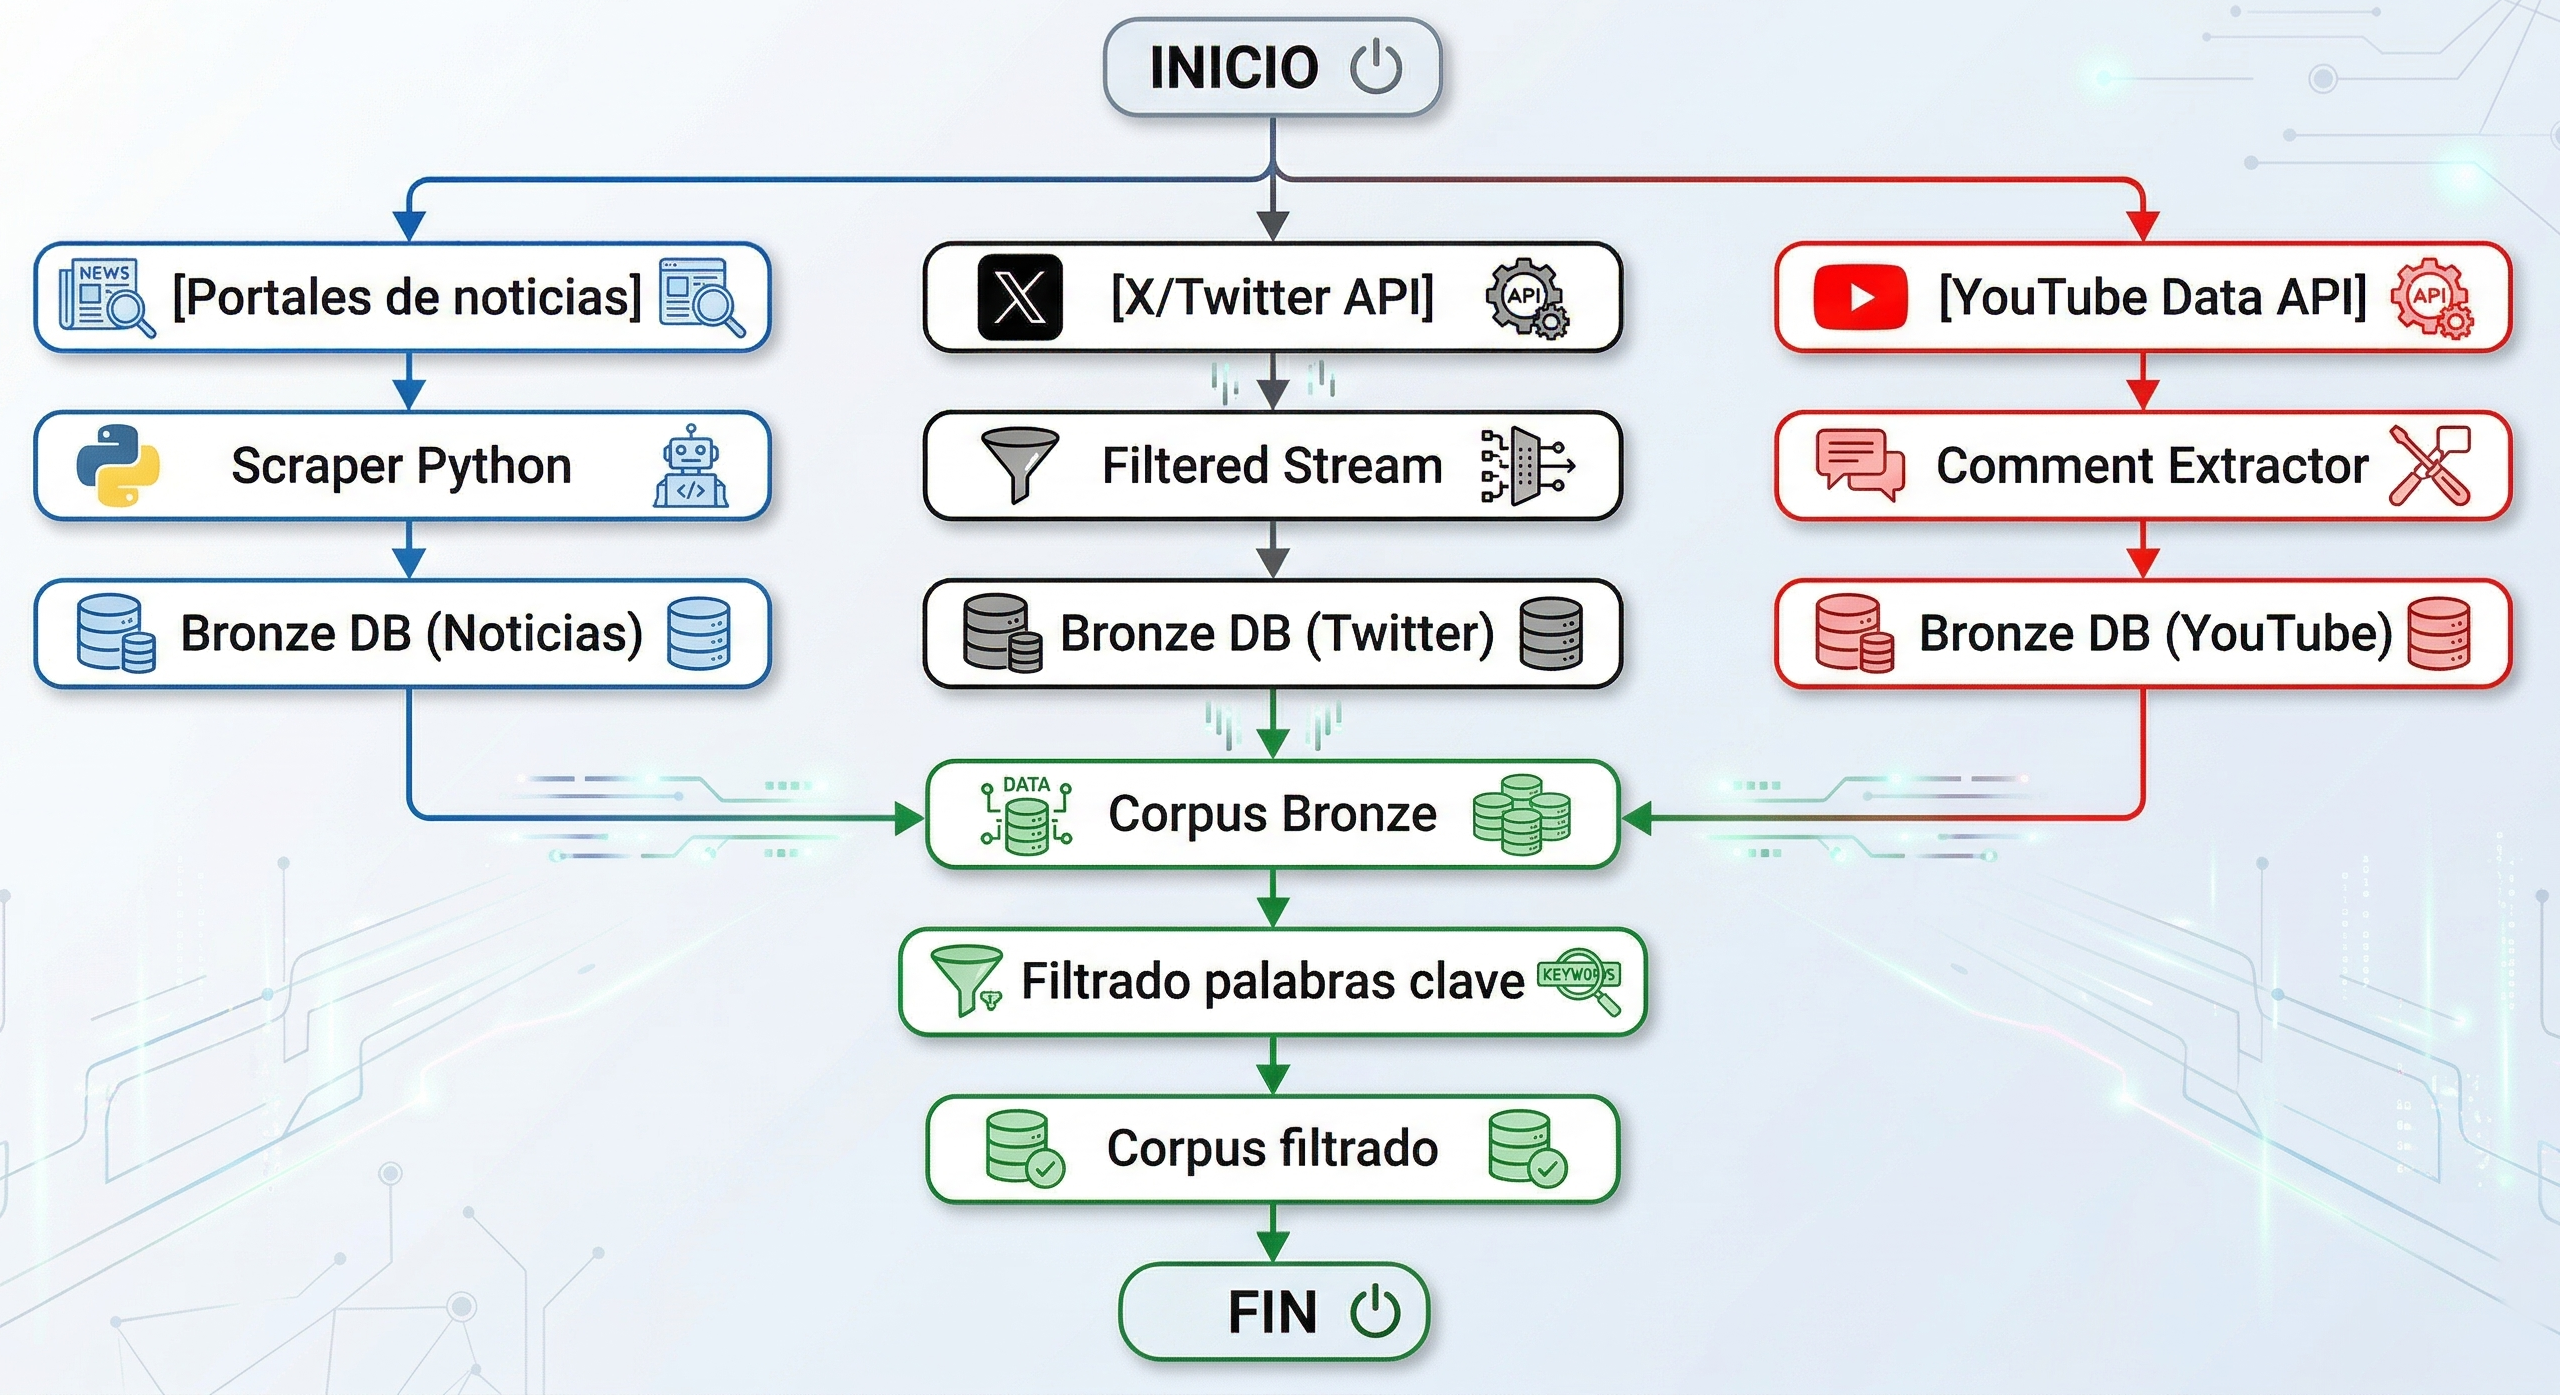
\includegraphics[width=0.90\textwidth]{images/flujo_recoleccion.png}
        \caption[Flujograma de recolección de los conjuntos de datos del corpus electoral]{Flujograma de recolección de los conjuntos de datos del corpus electoral: noticias digitales, comentarios de YouTube y tweets de X/Twitter, con sus respectivos procesos de filtrado y almacenamiento en la capa Bronze de la arquitectura Medallion.\\
            Fuente: Elaboración propia.}
        \label{4:fig1}
    \end{center}
\end{figure}
 
Asimismo, para identificar y filtrar las publicaciones relevantes para el análisis, se
definió un diccionario de palabras clave y aliases electorales que incluye los nombres
completos, apodos, partidos y hashtags de los candidatos presidenciales en liza, así como
términos relacionados con los principales temas de la campaña: economía, seguridad,
educación, salud, corrupción y gobernabilidad.
 
\section{Técnicas para el procesamiento y análisis de la información}
 
\subsection{Metodología de implementación de la solución}
 
Como se explicó en el Capítulo II del presente trabajo, dentro de los sistemas de
analítica de negocio, Big Data y Minería de Datos, las tres metodologías más usadas son
CRISP-DM, SEMMA y KDD \parencite{tec_braulio2015metodologiasdm}. Para elegir la
metodología de implementación, creamos la Tabla \ref{4:table2} con el propósito de comparar las variables empleadas por los autores en los antecedentes de esta investigación.
 
\vspace{2ex}
\begingroup
\renewcommand\arraystretch{1.2}
\small
\begin{longtable}{p{3cm}p{2.5cm}p{2.5cm}p{6cm}}
\caption[Cuadro comparativo para la selección de la metodología]{Cuadro comparativo para la selección de la metodología de implementación.}
\label{4:table2} \\
\specialrule{.1em}{.05em}{.05em}
\centering\textbf{Metodología} & \centering\textbf{Cantidad de referencias} & \centering\textbf{Número de pasos} & \centering\arraybackslash\textbf{Nombre de los pasos} \\
\specialrule{.1em}{.05em}{.05em}
\endfirsthead

% Este bloque se repetirá automáticamente si la tabla salta a la siguiente página
\caption[]{Cuadro comparativo para la selección de la metodología (continuación).} \\
\specialrule{.1em}{.05em}{.05em}
\centering\textbf{Metodología} & \centering\textbf{Cantidad de referencias} & \centering\textbf{Número de pasos} & \centering\arraybackslash\textbf{Nombre de los pasos} \\
\specialrule{.1em}{.05em}{.05em}
\endhead

CRISP-DM
& 2
& 6
& \begin{itemize}[label={--},nosep,leftmargin=*]
\item Entendimiento del negocio.
\item Análisis de los datos.
\item Preparación de la información.
\item Construcción del modelo.
\item Validación.
\item Implementación.
\end{itemize} \\ 
\hline
Grupo A
& 2
& 6
& \begin{itemize}[label={--},nosep,leftmargin=*]
\item Planteamiento del problema.
\item Obtención de datos multicanal.
\item Preprocesamiento de texto.
\item Análisis con LLM.
\item Evaluación.
\item Despliegue.
\end{itemize} \\ 
\hline
Grupo B
& 2
& 5
& \begin{itemize}[label={--},nosep,leftmargin=*]
\item Obtención de datos.
\item Preprocesamiento y filtrado.
\item Análisis de sentimientos.
\item Detección de temas.
\item Evaluación.
\end{itemize} \\ 
\hline
Grupo C
& 2
& 5
& \begin{itemize}[label={--},nosep,leftmargin=*]
\item Planteamiento del problema.
\item Obtención de datos.
\item Preprocesamiento de datos.
\item Modelado y análisis.
\item Evaluación.
\end{itemize} \\ 
\hline
Grupo D
& 1
& 4
& \begin{itemize}[label={--},nosep,leftmargin=*]
\item Obtención de datos.
\item Preprocesamiento.
\item Análisis LLM y clustering.
\item Evaluación.
\end{itemize} \\ 
\specialrule{.1em}{.05em}{.05em}
\end{longtable}
\endgroup
\begin{flushleft}
    \small Fuente: Elaboración propia.
\end{flushleft}
 
De las tres metodologías señaladas por \citeauthor{tec_braulio2015metodologiasdm}, la mayor parte de los antecedentes analizados siguen secuencias de actividades enmarcadas en CRISP-DM, abarcando etapas como la comprensión del negocio, la recolección y preparación de datos, el modelado y la evaluación. Asimismo, las siguientes características identificadas en la literatura influyeron en la selección de la metodología CRISP-DM para el presente estudio:

 
\begin{itemize}
    \item La metodología contempla entre sus fases la comprensión del negocio además
    de la parte técnica. Esta fase es crucial ya que en ella se define el problema a resolver
    —la falta de un sistema de análisis automatizado de percepción pública electoral en
    tiempo real— y se establecen los objetivos del sistema.
 
    \item Ayuda a los responsables del proyecto en la planificación y toma de decisiones
    (fase de Despliegue) a partir de los resultados obtenidos, convirtiendo los indicadores
    del sistema en oportunidades para mejorar la campaña de inteligencia electoral.
 
    \item Permite evaluar de manera continua los datos y las configuraciones del modelo a lo largo de todo el proceso, con el objetivo de construir el pipeline más adecuado. Estas evaluaciones resultan clave para interpretar los resultados y tomar decisiones sobre la arquitectura del sistema.

\item A diferencia de SEMMA, que inicia directamente con el muestreo sin enfatizar la comprensión del contexto, y de KDD, cuyo enfoque es más técnico y centrado en métricas sin considerar el entorno del negocio, CRISP-DM incorpora de forma explícita la formulación del problema, aspecto presente en el desarrollo de este trabajo.

\end{itemize}
 
Todas las etapas de la metodología que hemos escogido, adaptada al contexto de la
inteligencia electoral con LLMs, lo describimos en la Figura \ref{4:fig2}.
 
\begin{figure}[!ht]
    \begin{center}
        \includegraphics[width=1\textwidth]{images/metodologia_crispdm.png}
        \caption[Metodología CRISP-DM adaptada al sistema de inteligencia electoral con LLMs]{Metodología CRISP-DM adaptada al sistema de inteligencia electoral con LLMs, mostrando las seis fases, su carácter iterativo y los entregables de cada etapa.\\
            Fuente: Elaboración propia.}
        \label{4:fig2}
    \end{center}
\end{figure}
 
Durante la ejecución de la metodología, se definió construir un pipeline
de análisis multicanal que integra análisis de sentimientos con LLMs, detección dinámica
de temas con BERTopic y un grafo de conocimiento con Neo4j, arquitectura denominada
\textbf{Pipeline de Inteligencia Electoral Basado en LLMs y Grafo de Conocimiento}. De acuerdo a la literatura de los antecedentes revisados,
se analizaron las siguientes posibles fuentes de datos a incorporar:
 
\begin{itemize}
    \item \textbf{Noticias digitales}: \cite{pr_alvarez2023llm_political}, \cite{pr_mendonca2025bertopic_political}, \cite{pr_alvi2023twitter_election_review}.
    \item \textbf{Publicaciones en X/Twitter}: \cite{pr_gujral2024llm_elections}, \cite{pr_alvi2023twitter_election_review}, \cite{pr_mendonca2025bertopic_political}.
    \item \textbf{Comentarios de YouTube}: \cite{pr_chen2024combating_misinformation}.
    \item \textbf{Datos de encuestas electorales}: \cite{pr_gujral2024llm_elections}.
\end{itemize}
 
De las anteriores fuentes, los datos de encuestas electorales no fueron incluidos en el
pipeline principal de procesamiento ya que se utilizan exclusivamente como conjunto de
validación para calibrar los indicadores del sistema, y no como datos de entrada para el
análisis de sentimientos. Finalmente, fueron seleccionadas las tres fuentes principales
—noticias digitales, X/Twitter y comentarios de YouTube— cuya arquitectura de
recolección, procesamiento y análisis se detalla en las subsecciones siguientes.
 
El marco de trabajo del sistema propuesto, denominado \textbf{Pipeline GraphRAG
Electoral}, se estructura según la arquitectura Medallion en tres capas de datos
(Bronze, Silver y Gold) y cinco etapas de procesamiento, como vemos en la
Figura \ref{4:fig3}.
 
\begin{figure}[!ht]
    \begin{center}
        \includegraphics[width=0.92\textwidth]{images/framework_graphrag.png}
        \caption[Marco de trabajo del Pipeline GraphRAG Electoral propuesto]{Marco de trabajo del Pipeline GraphRAG Electoral: arquitectura Medallion con tres capas de datos (Bronze, Silver, Gold) y cinco etapas de procesamiento desde la ingesta hasta la generación de indicadores de percepción pública.\\
            Fuente: Elaboración propia.}
        \label{4:fig3}
    \end{center}
\end{figure}
 
\subsubsection{Entendimiento del negocio}
 
En la fase inicial, se definió el problema a partir de la comprensión del contexto del proceso electoral peruano y la necesidad de contar con un sistema automatizado de inteligencia electoral. Las actividades y tareas correspondientes a esta etapa se detallan en la Tabla \ref{4:table3}.

 
\vspace{2ex}
\begingroup
\renewcommand\arraystretch{1.2} 
\small 
\begin{longtable}{p{5cm}p{5cm}p{5cm}} 
\caption[Plan de Ejecución de la fase Entendimiento del negocio]{Plan de Ejecución de la fase Entendimiento del negocio.}
\label{4:table3} \\ 
\specialrule{.1em}{.05em}{.05em}
\centering\textbf{Plan de Ejecución} & \centering\textbf{Alcance} & \centering\arraybackslash\textbf{Acciones} \\
\specialrule{.1em}{.05em}{.05em}
\endfirsthead

% Esto aparecerá automáticamente si la tabla salta a una nueva página
\caption[]{Plan de Ejecución de la fase Entendimiento del negocio (continuación).} \\
\specialrule{.1em}{.05em}{.05em}
\centering\textbf{Plan de Ejecución} & \centering\textbf{Alcance} & \centering\arraybackslash\textbf{Acciones} \\
\specialrule{.1em}{.05em}{.05em}
\endhead

Plantear el problema, los objetivos y las hipótesis.
& Planteamiento del problema principal, así como de los objetivos generales y específicos y las hipótesis de investigación.
& \begin{itemize}[label={--},nosep,leftmargin=*]
\item Identificar la brecha existente en el análisis de la percepción electoral digital.
\item Establecer los objetivos del sistema de inteligencia electoral.
\item Formular las hipótesis del estudio.
\end{itemize} \\ 
\hline
Desarrollar el marco teórico de la investigación.
& Revisión de estudios previos relacionados con el análisis de sentimientos en contextos políticos, LLMs y detección de temas.
& \begin{itemize}[label={--},nosep,leftmargin=*]
\item Buscar literatura académica sobre el uso de LLMs en escenarios electorales.
\item Revisar material sobre BERTopic y GraphRAG aplicado a datos políticos.
\end{itemize} \\ 
\hline
Definir la metodología y la arquitectura del sistema.
& Selección de la metodología de trabajo y diseño de la arquitectura del pipeline.
& \begin{itemize}[label={--},nosep,leftmargin=*]
\item Analizar metodologías propuestas en la literatura.
\item Escoger la metodología CRISP-DM.
\item Diseñar la arquitectura tipo Medallion del sistema.
\end{itemize} \\ 
\specialrule{.1em}{.05em}{.05em}
\end{longtable}
\endgroup
\begin{flushleft}
\small Fuente: Elaboración propia.
\end{flushleft}
 
\textbf{Actividad 1: Plantear el problema, los objetivos e hipótesis}
 
Aquí vemos la manera en que identificamos la brecha existente en el análisis automatizado de la percepción pública electoral digital en el Perú, se formularon los objetivos de la investigación y se plantearon las hipótesis que guían el trabajo experimental.
 
\textbf{Entregable}: Problema, objetivos e hipótesis definidos.
 
\textbf{Actividad 2: Desarrollar el marco teórico de la investigación}
 
Ya con los objetivos definidos, realizamos la investigación de antecedentes académicos relacionados con el uso de LLMs en contextos electorales, minería de sentimientos político en español, detección dinámica de temas con BERTopic y sistemas GraphRAG. Se elaboró el marco teórico y conceptual descritos en el Capítulo II del presente trabajo.
 
\textbf{Entregable}: Marco teórico, antecedentes y conceptos operacionales de la investigación.
 
\textbf{Actividad 3: Definir metodología y arquitectura del sistema}
 
Luego de revisar los antecedentes y comparar las metodologías utilizadas por cada autor, se seleccionó CRISP-DM como metodología de implementación y se diseñó la arquitectura Medallion del pipeline GraphRAG Electoral.
 
\textbf{Entregable}: Metodología de implementación y arquitectura del sistema.
 
\subsubsection{Análisis de los datos}
 
En la segunda fase se llevó a cabo la recolección de datos y el análisis estadístico exploratorio del corpus electoral multicanal. La información empleada incluye publicaciones provenientes de tres fuentes principales, recopiladas durante el período de campaña presidencial. Las actividades y tareas correspondientes se detallan en la Tabla \ref{4:table4}.
 
\vspace{2ex}
\begingroup
\renewcommand\arraystretch{1.2}
\small
\begin{longtable}{p{4cm}p{5.5cm}p{5.5cm}}
\caption[Plan de Ejecución de la fase Análisis de los datos]{Plan de Ejecución de la fase Análisis de los datos.}
\label{4:table4} \\
\specialrule{.1em}{.05em}{.05em}
\centering\textbf{Plan de Ejecución} & \centering\textbf{Alcance} & \centering\arraybackslash\textbf{Acciones} \\
\specialrule{.1em}{.05em}{.05em}
\endfirsthead

% Este bloque se repetirá automáticamente si la tabla salta a la siguiente página
\caption[]{Plan de Ejecución de la fase Análisis de los datos (continuación).} \\
\specialrule{.1em}{.05em}{.05em}
\centering\textbf{Plan de Ejecución} & \centering\textbf{Alcance} & \centering\arraybackslash\textbf{Acciones} \\
\specialrule{.1em}{.05em}{.05em}
\endhead

Construir corpus de noticias digitales.
& Construcción del corpus de artículos y titulares de los principales portales de prensa peruanos (capa Bronze).
& \begin{itemize}[label={--},nosep,leftmargin=*]
\item Diseñar scrapers para portales de noticias objetivo.
\item Recolectar artículos con URL, fecha, titular y texto.
\item Almacenar datos crudos en capa Bronze.
\end{itemize} \\ 
\hline
Construir corpus de X/Twitter.
& Construcción del corpus de tweets relacionados con los candidatos presidenciales mediante la API de X.
& \begin{itemize}[label={--},nosep,leftmargin=*]
\item Configurar conexión con la API Filtered Stream de X.
\item Definir palabras clave, hashtags y cuentas de interés.
\item Almacenar tweets con metadatos en capa Bronze.
\end{itemize} \\ 
\hline
Construir corpus de YouTube.
& Construcción del corpus de comentarios de usuarios en videos electorales de YouTube.
& \begin{itemize}[label={--},nosep,leftmargin=*]
\item Identificar videos electorales mediante YouTube Data API.
\item Recolectar comentarios con ID de usuario y fecha.
\item Almacenar comentarios crudos en capa Bronze.
\end{itemize} \\ 
\hline
Realizar análisis exploratorio del corpus.
& Análisis estadístico y exploratorio de las variables del corpus para cada fuente de datos.
& \begin{itemize}[label={--},nosep,leftmargin=*]
\item Describir distribución temporal y por fuente.
\item Analizar longitud de textos y vocabulario.
\item Identificar candidatos más mencionados.
\end{itemize} \\ 
\specialrule{.1em}{.05em}{.05em}
\end{longtable}
\endgroup
\begin{flushleft}
    \small Fuente: Elaboración propia.
\end{flushleft}
 
\textbf{Actividad 1: Construir corpus de noticias digitales}
 
De acuerdo a la Figura \ref{4:fig1}, en esta actividad se construyó el corpus de artículos de noticias digitales mediante scrapers diseñados en Python para los portales de prensa peruanos seleccionados. El proceso de recolección siguió el flujo de la Figura \ref{4:fig4}.
 
\begin{figure}[!ht]
    \begin{center}
        \includegraphics[width=0.80\textwidth]{images/flujo_scraping_noticias.png}
        \caption[Proceso de recolección del corpus de noticias digitales]{Proceso de recolección del corpus de noticias digitales: desde la identificación de portales objetivo hasta el almacenamiento en la capa Bronze de la arquitectura Medallion.\\
            Fuente: Elaboración propia.}
        \label{4:fig4}
    \end{center}
\end{figure}
 
\textbf{Entregable}: Corpus de noticias digitales con URL, fecha, portal de origen, titular y texto completo del artículo.
 
\textbf{Actividad 2: Construir corpus de X/Twitter}
 
La recolección de tweets se realizó mediante TwitterAPI.io, un proveedor de acceso a datos de Twitter/X que expone una API REST compatible con los principales endpoints de búsqueda y usuario. A diferencia de la API oficial de X/Twitter —cuyo plan Basic tiene un costo de \$100/mes con limitación de 10,000 tweets mensuales—, TwitterAPI.io permite una recolección más flexible durante el período de campaña electoral. El cliente Python desarrollado en src/electoral/ingestion/twitter.py consume esta API de forma asíncrona mediante \texttt{httpx}, filtrando los resultados por \texttt{date\_from}/\texttt{date\_to} con tolerancia de $\pm1$ día respecto a la fecha de publicación.

\begin{figure}[!ht]
    \begin{center}
        \includegraphics[width=0.80\textwidth]{images/flujo_api_twitter.png}
        \caption[Proceso de recolección del corpus de X/Twitter mediante API Filtered Stream]{Proceso de recolección del corpus de X/Twitter: configuración de reglas de filtrado, captura en streaming y almacenamiento con metadatos en capa Bronze.\\
            Fuente: Elaboración propia.}
        \label{4:fig5}
    \end{center}
\end{figure}
 
\textbf{Entregable}: Corpus de tweets con ID, texto, fecha, número de retweets y menciones a candidatos.
 
\textbf{Actividad 3: Construir corpus de YouTube}
 
La recolección de contenido de YouTube se realizó mediante \texttt{yt-dlp}, una herramienta de scraping de video de código abierto que extrae metadata, transcripciones y comentarios de videos de YouTube sin depender de cuotas de la API oficial. El ingestor (src/electoral/ingestion/youtube.py) implementa un patrón productor-consumidor con hilos paralelos: un hilo extrae los IDs de videos en lotes (\textit{extract\_flat}), y múltiples hilos trabajadores obtienen la metadata completa y filtran por fecha de publicación. Las transcripciones se marcan con el flag \texttt{is\_auto\_generated} para distinguir subtítulos automáticos de los manuales. El pool de cookies Netscape del directorio \texttt{cookies/} es distribuido entre los workers por round-robin para reducir bloqueos.

\begin{figure}[!ht]
    \begin{center}
        \includegraphics[width=0.80\textwidth]{images/flujo_youtube_comentarios.png}
        \caption[Proceso de recolección del corpus de comentarios de YouTube]{Proceso de extracción de comentarios de usuarios en videos electorales de YouTube, desde la identificación de videos relevantes hasta el almacenamiento en capa Bronze.\\
            Fuente: Elaboración propia.}
        \label{4:fig6}
    \end{center}
\end{figure}
 
\textbf{Entregable}: Corpus de comentarios de YouTube con ID de video, texto del comentario, fecha y número de likes.
 
\textbf{Actividad 4: Realizar análisis exploratorio del corpus}
 
En esta actividad se realizó el análisis estadístico descriptivo de los tres corpus recolectados: distribución temporal de publicaciones, longitud promedio de textos, distribución de menciones por candidato y por fuente, y análisis del vocabulario electoral dominante mediante nubes de palabras.
 
\textbf{Entregable}: Gráficos estadísticos y descriptivos del corpus por fuente de datos.
 
\subsubsection{Preparación de la información}
 
En la tercera fase, los datos crudos de la capa Bronze se transformaron en la capa Silver
mediante un conjunto de procesos de limpieza, normalización y enriquecimiento. Las
actividades de esta etapa se detallan en la Tabla \ref{4:table5}.
 
\vspace{2ex}
\begingroup
\renewcommand\arraystretch{1.2}
\small
\begin{longtable}{p{5cm}p{5cm}p{5cm}}
\caption[Plan de Ejecución de la fase Preparación de la información]{Plan de Ejecución de la fase Preparación de la información.}
\label{4:table5} \\
\specialrule{.1em}{.05em}{.05em}
\centering\textbf{Plan de Ejecución} & \centering\textbf{Alcance} & \centering\arraybackslash\textbf{Acciones} \\
\specialrule{.1em}{.05em}{.05em}
\endfirsthead

% Este bloque se repetirá automáticamente si la tabla salta a la siguiente página
\caption[]{Plan de Ejecución de la fase Preparación de la información (continuación).} \\
\specialrule{.1em}{.05em}{.05em}
\centering\textbf{Plan de Ejecución} & \centering\textbf{Alcance} & \centering\arraybackslash\textbf{Acciones} \\
\specialrule{.1em}{.05em}{.05em}
\endhead

Limpiar y normalizar el corpus.
& Preprocesamiento textual de las publicaciones de las tres fuentes para su análisis con LLM.
& \begin{itemize}[label={--},nosep,leftmargin=*]
\item Eliminar spam, bots y publicaciones duplicadas.
\item Normalizar caracteres especiales, emojis y URLs.
\item Detectar y filtrar publicaciones en idiomas distintos al español.
\end{itemize} \\ 
\hline
Segmentar el corpus para análisis.
& División de textos largos en segmentos procesables por el LLM respetando la ventana de contexto.
& \begin{itemize}[label={--},nosep,leftmargin=*]
\item Definir tamaño máximo de segmento en tokens.
\item Implementar segmentación con superposición de contexto.
\item Registrar relación documento-segmento en base de datos.
\end{itemize} \\ 
\hline
Construir diccionario de aliases electorales.
& Creación del diccionario de names, apodos y aliases de candidatos para el filtrado con Aho-Corasick.
& \begin{itemize}[label={--},nosep,leftmargin=*]
\item Recopilar nombres completos y apodos de candidatos.
\item Incluir nombres de partidos y lemas de campaña.
\item Construir el autómata Aho-Corasick para búsqueda eficiente.
\end{itemize} \\ 
\specialrule{.1em}{.05em}{.05em}
\end{longtable}
\endgroup
\begin{flushleft}
    \small Fuente: Elaboración propia.
\end{flushleft}
 
\textbf{Actividad 1: Limpiar y normalizar el corpus}
 
En esta actividad se aplicó un pipeline de preprocesamiento textual sobre los tres corpus de la capa Bronze. El proceso incluyó la eliminación de spam y cuentas de bots identificadas mediante patrones de comportamiento, la normalización de emojis (convertidos a texto descriptivo), la eliminación de URLs y menciones de usuario, y la detección automática de idioma mediante la librería \texttt{langdetect} para conservar únicamente publicaciones en español.
 
\textbf{Entregable}: Corpus limpio y normalizado, listo para análisis con LLM.
 
\textbf{Actividad 2: Segmentar el corpus para análisis}
 
Dado que los artículos de noticias superan en longitud la ventana de contexto del LLM utilizado, se implementó un proceso de segmentación con superposición que divide cada documento en segmentos de máximo 512 tokens con una superposición de 50 tokens entre segmentos consecutivos, preservando el contexto necesario para el análisis de sentimientos a nivel de aspecto.
 
\textbf{Entregable}: Tabla de segmentos con relación uno-a-muchos hacia la tabla de documentos originales (capa Silver).
 
\textbf{Actividad 3: Construir diccionario de aliases electorales}
 
Se construyó el diccionario de aliases que alimenta el autómata Aho-Corasick descrito en el pipeline. Este diccionario incluye los nombres completos, apodos, partidos políticos y lemas de campaña de todos los candidatos presidenciales, permitiendo detectar menciones implícitas y coloquiales que un buscador de texto exacto no capturaría. Este paso es fundamental para garantizar que el LLM solo analice segmentos que efectivamente contienen referencias a candidatos, reduciendo el costo computacional en un factor proporcional al número de aliases registrados.
 
\textbf{Entregable}: Diccionario de aliases y autómata Aho-Corasick compilado.
 
\subsubsection{Construcción del modelo}
 
Al concluir la preparación de los datos, los segmentos del corpus enriquecido fueron
procesados por el pipeline de análisis con LLMs. Las actividades de esta fase se detallan
en la Tabla \ref{4:table6}.
 
\vspace{2ex}
\begingroup
\renewcommand\arraystretch{1.2}
\small
\begin{longtable}{p{4.6cm}p{4.9cm}p{5.5cm}}
\caption[Plan de Ejecución de la fase Construcción del modelo]{Plan de Ejecución de la fase Construcción del modelo.}
\label{4:table6} \\
\specialrule{.1em}{.05em}{.05em}
\centering\textbf{Plan de Ejecución} & \centering\textbf{Alcance} & \centering\arraybackslash\textbf{Acciones} \\
\specialrule{.1em}{.05em}{.05em}
\endfirsthead

% Este bloque se repetirá automáticamente si la tabla salta a la siguiente página
\caption[]{Plan de Ejecución de la fase Construcción del modelo (continuación).} \\
\specialrule{.1em}{.05em}{.05em}
\centering\textbf{Plan de Ejecución} & \centering\textbf{Alcance} & \centering\arraybackslash\textbf{Acciones} \\
\specialrule{.1em}{.05em}{.05em}
\endhead

Construir módulo de análisis de sentimientos con LLM.
& Implementación del análisis de sentimientos a nivel de aspecto mediante prompts diseñados para el contexto electoral peruano.
& \begin{itemize}[label={--},nosep,leftmargin=*]
\item Diseñar prompt de análisis con estructura role-context-task-format.
\item Implementar llamadas a la API del LLM con respuesta JSON estructurada.
\item Validar outputs y gestionar errores de parsing.
\end{itemize} \\ 
\hline
Desarrollar módulo de detección dinámica de temas.
& Implementación del pipeline BERTopic para clustering semántico de temas electorales.
& \begin{itemize}[label={--},nosep,leftmargin=*]
\item Generar embeddings con Sentence-BERT multilingüe.
\item Reducir dimensionalidad con UMAP.
\item Aplicar HDBSCAN para clustering inductivo.
\item Etiquetar clusters con LLM mediante c-TF-IDF.
\end{itemize} \\ 
\hline
Construir grafo de conocimiento electoral.
& Implementación del grafo Neo4j con nodos y relaciones del ecosistema electoral digital.
& \begin{itemize}[label={--},nosep,leftmargin=*]
\item Definir esquema de nodos (Candidato, Tema, Fuente, Periodo, Evento).
\item Implementar jobs de agregación semanal con MERGE idempotente.
\item Calcular relaciones MENCIONA, CO\_OCURRE, CUBRE y REACCIONA\_A.
\end{itemize} \\ 
\hline
Implementar sistema GraphRAG para consultas.
& Desarrollo del módulo de consulta en lenguaje natural sobre el grafo de conocimiento electoral.
& \begin{itemize}[label={--},nosep,leftmargin=*]
\item Inyectar schema del grafo al contexto del LLM.
\item Implementar traducción de preguntas en español a consultas Cypher.
\item Validar respuestas con evidencia textual de los documentos originales.
\end{itemize} \\ 
\specialrule{.1em}{.05em}{.05em}
\end{longtable}
\endgroup
\begin{flushleft}
    \small Fuente: Elaboración propia.
\end{flushleft}
 
\textbf{Actividad 1: Desarrollar módulo de análisis de sentimientos con LLM}
 
En esta actividad se diseñó el prompt de análisis de sentimientos a nivel de aspecto y se
implementó el módulo de llamadas a la API del LLM. El prompt sigue la estructura de
cinco componentes (rol, contexto, instrucción, formato y ejemplos few-shot) descrita en el
marco conceptual, y extrae en una sola llamada por segmento: candidatos detectados,
método de detección, nivel de confianza, score de sentimiento en escala $[-1, 1]$,
fragmento clave que justifica el sentimiento, temas identificados y relaciones entre temas.
Para la selección del LLM, se realizó un benchmarking sobre las propuestas de los
autores de los antecedentes:
 
\begin{itemize}
    \item \textbf{Gemini (Google)}: \cite{pr_alvarez2023llm_political}, arquitectura del HTML de metodología adjunto.
    \item \textbf{GPT-4 (OpenAI)}: \cite{pr_gujral2024llm_elections}, \cite{pr_chen2024combating_misinformation}.
    \item \textbf{Llama 2 (Meta, código abierto)}: \cite{pr_gujral2024llm_elections}.
    \item \textbf{mBERT / XLM-RoBERTa (modelos encoder)}: \cite{pr_alvi2023twitter_election_review}.
\end{itemize}
 
Para la selección del modelo LLM, se evaluaron las alternativas propuestas en los antecedentes de la investigación. A diferencia de lo inicialmente planificado con Gemini Flash como modelo principal, el sistema implementado seleccionó DeepSeek-Chat como proveedor LLM principal, con Gemini Flash como fallback configurable mediante la variable de entorno \texttt{LLM\_PROVIDER}. La decisión se fundamentó en tres factores: (1) el mecanismo de caché de prefijo transparente de DeepSeek, que descuenta hasta el 75\% del costo en tokens de entrada para el prefijo invariante del prompt (catálogos, instrucciones y ejemplos few-shot), alcanzando un 85.5\% de \textit{cache hit} sostenido; (2) el soporte nativo de \texttt{response\_format: JSON} que garantiza outputs parseables por Pydantic sin prompting heroico; y (3) un costo por documento aproximadamente 10 veces menor que GPT-4o para el mismo volumen. La abstracción \texttt{LLMClient} (\texttt{src/electoral/llm/clients/base.py}) permite intercambiar el proveedor con un cambio de variable de entorno, por lo que los experimentos de validación con GPT-4o se realizaron sin modificar el código del pipeline.
 
\textbf{Entregable}: Módulo de análisis de sentimientos con LLM y tabla \texttt{analisis} de la capa Silver.
 
\textbf{Actividad 2: Desarrollar módulo de detección dinámica de temas}
 
A diferencia del enfoque BERTopic propuesto inicialmente, el sistema implementado utiliza una estrategia de detección de temas emergentes dirigida por LLM con catálogo incremental. En cada llamada de análisis, el LLM recibe un menú de hasta 20 temas candidatos construido mediante cinco tiers de retrieval sobre el catálogo existente en PostgreSQL: (1) temas trending por volumen, (2) búsqueda semántica por cosine sobre pgvector, (3) coincidencia léxica con el título y cuerpo del documento, (4) temas asociados al actor protagonista detectado, y (5) temas del catálogo de eventos conocidos.

El LLM indica si el documento corresponde a un tema existente (\texttt{exact}), a un alias de uno existente (\texttt{alias}), o a un tema nuevo (\texttt{new}). Esta arquitectura permite la detección dinámica de temas emergentes sin reentrenamiento de modelos y con un costo marginal aproximado de 50 tokens adicionales por documento.

Los temas se consolidan posteriormente mediante dos procesos: \texttt{consolidate\_day}, basado en matching threshold-based con similitud cosine $\geq 0.78$, y \texttt{llm\_dedup\_day}, que realiza deduplicación semántica mediante evaluación LLM sobre pares sospechosos, limitado a un máximo de 200 pares por día.

Asimismo, la regla número cinco del prompt maneja automáticamente publicaciones no políticas —como deportes, entretenimiento, farándula o humor/sátira— asignándoles es\_relevante=false y clasificándolas dentro de categorías fijas del tipo \texttt{otros\_<categoria>}, evitando inflar el catálogo de temas con ruido semántico.
 
\textbf{Entregable}: Pipeline BERTopic configurado y taxonomía de temas electorales generada.
 
\textbf{Actividad 3: Construir grafo de conocimiento electoral}
 
En esta actividad se implementó el grafo de conocimiento electoral en Neo4j utilizando un esquema compuesto por los labels: \texttt{Documento}, \texttt{Fragmento}, \texttt{Tema}, \texttt{Actor}, \texttt{Candidato}, \texttt{Categoria}, \texttt{Encuesta}, \texttt{SentimientoDiario}, \texttt{TipoCambio} e \texttt{IndicadorMacro}. Las relaciones implementadas fueron: \texttt{CONTIENE}, \texttt{SOBRE\_TEMA}, \texttt{MENCIONA}, \texttt{MENCIONA\_ACTOR}, \texttt{DE\_CATEGORIA}, \texttt{MIDE} y \texttt{TIENE\_SENTIMIENTO\_EN}.

A diferencia del diseño conceptual inicial, el sistema implementado no utiliza el nodo \texttt{Periodo} ni las relaciones \texttt{CO\_OCURRE}, \texttt{CUBRE}, \texttt{SILENCIA} o \texttt{REACCIONA\_A}. El pipeline de agregación actualiza los nodos y relaciones mediante operaciones idempotentes sobre Neo4j para evitar duplicación de información durante la reejecución de procesos ETL.
 
\textbf{Entregable}: Grafo de conocimiento electoral en Neo4j con datos agregados semanalmente.
 
\textbf{Actividad 4: Implementar sistema GraphRAG para consultas}
 
El módulo de consulta al grafo de conocimiento se implementó como un servidor MCP (\textit{Model Context Protocol}) mediante el framework FastMCP 3.2.4, utilizando transporte \texttt{streamable-http} sobre el puerto 8080. El servidor expone 13 herramientas tipadas que los clientes LLM —como Claude Desktop y Claude.ai— pueden invocar directamente durante una conversación:

\begin{itemize}
    \item \texttt{contexto\_candidato}
    \item \texttt{evolucion\_sentimiento\_candidato}
    \item \texttt{comparar\_candidatos\_sentimiento}
    \item \texttt{temas\_top\_periodo}
    \item \texttt{buscar\_tema\_por\_descripcion}
    \item \texttt{buscar\_actor\_por\_descripcion}
    \item \texttt{noticias\_por\_actor}
    \item \texttt{citar\_evidencia}
    \item \texttt{panorama\_diario}
    \item \texttt{intencion\_voto\_candidato}
    \item \texttt{encuestas\_disponibles}
    \item \texttt{tipo\_cambio\_periodo}
    \item \texttt{indicador\_macro\_periodo}
\end{itemize}

Cada herramienta valida sus entradas y salidas mediante esquemas Pydantic v2, mientras que el \texttt{outputSchema} JSON generado automáticamente permite validación estricta por parte del cliente consumidor. La autenticación del servidor se implementó mediante Bearer Token con comparación en tiempo constante utilizando \texttt{hmac.compare\_digest}, reduciendo la posibilidad de ataques de temporización.
 
\textbf{Entregable}: Módulo GraphRAG funcional con ejemplos de consultas en lenguaje natural validados.
 
\subsubsection{Validación}
 
Esta fase incluye la evaluación del sistema de inteligencia electoral mediante las métricas seleccionadas de clasificación y calidad de temas. Las actividades y tareas desarrolladas se presentan en la Tabla \ref{4:table7}.

 
\begingroup
\renewcommand\arraystretch{1.2}
\small
\begin{longtable}{p{5cm}p{4.5cm}p{5.5cm}}
\caption[Plan de Ejecución de la fase Validación]{Plan de Ejecución de la fase Validación.}
\label{4:table7} \\
\specialrule{.1em}{.05em}{.05em}
\centering\textbf{Plan de Ejecución} & \centering\textbf{Alcance} & \centering\arraybackslash\textbf{Acciones} \\
\specialrule{.1em}{.05em}{.05em}
\endfirsthead

% Este bloque se repetirá automáticamente si la tabla salta a la siguiente página
\caption[]{Plan de Ejecución de la fase Validación (continuación).} \\
\specialrule{.1em}{.05em}{.05em}
\centering\textbf{Plan de Ejecución} & \centering\textbf{Alcance} & \centering\arraybackslash\textbf{Acciones} \\
\specialrule{.1em}{.05em}{.05em}
\endhead

Evaluar módulo de análisis de sentimientos.
& Evaluación del desempeño del análisis de sentimientos comparando los resultados del LLM con etiquetas humanas de referencia.
& \begin{itemize}[label={--},nosep,leftmargin=*]
\item Construir conjunto de validación con etiquetas humanas.
\item Calcular exactitud, precisión, sensibilidad y F1.
\item Comparar resultados entre distintas configuraciones de prompt.
\end{itemize} \\ 
\hline
Evaluar módulo de detección de temas.
& Evaluación de la coherencia semántica y diversidad de los temas detectados por BERTopic.
& \begin{itemize}[label={--},nosep,leftmargin=*]
\item Calcular coherencia C\textsubscript{v} de los temas.
\item Evaluar diversidad temática del corpus.
\item Validar etiquetas de clusters con analistas políticos.
\end{itemize} \\ 
\hline
Evaluar sistema GraphRAG.
& Evaluación de la precisión de las consultas Cypher generadas y la calidad de las respuestas en lenguaje natural.
& \begin{itemize}[label={--},nosep,leftmargin=*]
\item Diseñar conjunto de preguntas de evaluación con respuesta esperada.
\item Medir exactitud de las consultas Cypher generadas.
\item Evaluar factualidad y trazabilidad de las respuestas.
\end{itemize} \\ 
\hline
Evaluar el sistema integrado.
& Evaluación del pipeline completo en términos de latencia, escalabilidad y correlación con encuestas de opinión.
& \begin{itemize}[label={--},nosep,leftmargin=*]
\item Medir latencia extremo a extremo del pipeline.
\item Comparar indicadores ISN con encuestas electorales disponibles.
\item Evaluar correlación de Pearson entre ambas fuentes.
\end{itemize} \\ 
\specialrule{.1em}{.05em}{.05em}
\end{longtable}
\endgroup
\begin{flushleft}
    \small Fuente: Elaboración propia.
\end{flushleft}
 
\subsubsection{Implementación}
 
En la fase final de la metodología, el sistema de inteligencia electoral se implementó como un prototipo funcional, accesible para analistas políticos y periodistas. Las actividades correspondientes a esta etapa se describen en la Tabla \ref{4:table8}.

 
\begingroup
\renewcommand\arraystretch{1.2}
\small
\begin{longtable}{p{4.5cm}p{5.3cm}p{5.2cm}}
\caption[Plan de Ejecución de la fase Implementación]{Plan de Ejecución de la fase Implementación.}
\label{4:table8} \\
\specialrule{.1em}{.05em}{.05em}
\centering\textbf{Plan de Ejecución} & \centering\textbf{Alcance} & \centering\arraybackslash\textbf{Acciones} \\
\specialrule{.1em}{.05em}{.05em}
\endfirsthead

% Este bloque se repetirá automáticamente si la tabla salta a la siguiente página
\caption[]{Plan de Ejecución de la fase Implementación (continuación).} \\
\specialrule{.1em}{.05em}{.05em}
\centering\textbf{Plan de Ejecución} & \centering\textbf{Alcance} & \centering\arraybackslash\textbf{Acciones} \\
\specialrule{.1em}{.05em}{.05em}
\endhead

Diseñar dashboard de visualización.
& Diseño e implementación del dashboard interactivo que muestra los indicadores de percepción pública en tiempo real.
& \begin{itemize}[label={--},nosep,leftmargin=*]
\item Diseñar vistas para ISN, IRT e IVE por candidato y período.
\item Implementar gráficos de evolución temporal y mapas de calor temáticos.
\item Integrar módulo de consulta GraphRAG en lenguaje natural.
\end{itemize} \\ 
\hline
Ejecutar prototipo con datos electorales en vivo.
& Ejecución del sistema completo en condiciones reales durante el período de campaña presidencial.
& \begin{itemize}[label={--},nosep,leftmargin=*]
\item Activar pipeline de ingesta en tiempo real.
\item Monitorear indicadores y detectar anomalías.
\item Generar reportes automáticos diarios.
\end{itemize} \\ 
\specialrule{.1em}{.05em}{.05em}
\end{longtable}
\endgroup
\begin{flushleft}
    \small Fuente: Elaboración propia.
\end{flushleft}
 
Tras evaluar el desempeño de cada módulo del sistema, se procedió a comparar los resultados con los antecedentes analizados y se llevó a cabo una prueba piloto, en la cual el sistema completo operó en tiempo real durante una semana de campaña electoral. Los detalles de esta prueba y sus resultados se presentan en el Capítulo V.
 
\subsection{Metodología para la medición de resultados}
 
Para evaluar el desempeño de los módulos del sistema, correspondiente a la quinta fase de la metodología CRISP-DM, se emplearon diversas métricas como instrumentos para medir su rendimiento. A continuación, se describen su definición y fórmulas de cálculo.
 
\begin{itemize}
    \item \textbf{Matriz de confusión}: Es una tabla de $N \times N$ que resume el nivel de
    éxito de las predicciones de un modelo de clasificación. Para el módulo de análisis de
    sentimientos, $N=3$ (positivo, negativo, neutral), permitiendo identificar los errores más
    frecuentes de clasificación (por ejemplo, confundir sentimiento neutro con negativo en
    textos irónicos) \parencite{gl_kohavi1998ml_glossary}.
 
    \item \textbf{Exactitud} (\textit{accuracy}): Fracción de predicciones de sentimiento
    realizadas correctamente sobre el total de publicaciones en el conjunto de validación.
    Se calcula mediante la Ecuación \ref{eq:accuracy_llm}:
 
    \begin{equation}\label{eq:accuracy_llm}
    \phantomsection
    Exactitud = \frac{V.P. + V.N.}{V.P. + V.N. + F.P. + F.N.}
    \end{equation}
    \myequations{Fórmula para calcular la exactitud del módulo de sentimientos}
 
    \item \textbf{Precisión} (\textit{precision}): Proporción de publicaciones clasificadas
    correctamente como de sentimiento positivo sobre el total de publicaciones clasificadas
    como positivas por el sistema. Se calcula mediante la Ecuación \ref{eq:precision_llm}:
 
    \begin{equation}\label{eq:precision_llm}
    \phantomsection
    Precisi\acute{o}n = \frac{V.P.}{V.P. + F.P.}
    \end{equation}
    \myequations{Fórmula para calcular la precisión del módulo de sentimientos}
 
    \item \textbf{Sensibilidad} (\textit{recall}): Proporción de publicaciones realmente
    positivas que el sistema identifica correctamente. Se calcula mediante la Ecuación
    \ref{eq:recall_llm}:
 
    \begin{equation}\label{eq:recall_llm}
    \phantomsection
    Sensibilidad = \frac{V.P.}{V.P. + F.N.}
    \end{equation}
    \myequations{Fórmula para calcular la sensibilidad del módulo de sentimientos}
 
    \item \textbf{Puntaje F1}: Se define como la media armónica entre la precisión y la sensibilidad. Se emplea especialmente cuando las clases de sentimiento se encuentran desbalanceadas —situación común en corpus electorales, donde el sentimiento negativo suele predominar sobre el positivo— y no es adecuado basar las conclusiones únicamente en la exactitud. Su cálculo se realiza mediante la Ecuación \ref{eq:f1_llm}:
 
    \begin{equation}\label{eq:f1_llm}
    \phantomsection
    Puntaje\ F1 = \frac{2 \times Precisi\acute{o}n \times Sensibilidad}{Precisi\acute{o}n + Sensibilidad}
    \end{equation}
    \myequations{Fórmula para calcular el puntaje F1 del módulo de sentimientos}
 
    \item \textbf{Coherencia semántica $C_v$}: Métrica estándar para evaluar la calidad de
    los temas generados por modelos de topic modeling. Mide la co-ocurrencia normalizada
    de los términos más representativos de cada tema en el corpus. Un valor de $C_v$
    cercano a 1 indica temas semánticamente coherentes. Se calcula mediante la Ecuación
    \ref{eq:cv_coherence}:
 
    \begin{equation}\label{eq:cv_coherence}
    \phantomsection
    C_v(t) = \frac{1}{\binom{|W|}{2}} \sum_{i>j} \log \frac{P(w_i, w_j) + \epsilon}{P(w_i) \cdot P(w_j)}
    \end{equation}
    \myequations{Fórmula para calcular la coherencia semántica $C_v$ de los temas detectados}
 
    Donde $W$ es el conjunto de los términos más representativos del tema $t$, $P(w_i, w_j)$
    es la probabilidad de co-ocurrencia de los términos $w_i$ y $w_j$ en el corpus, y
    $\epsilon$ es un suavizador para evitar logaritmos de cero.
 
    \item \textbf{Correlación de Pearson con encuestas}: Mide el grado de correlación
    lineal entre el Índice de Sentimiento Neto (ISN) calculado por el sistema para cada
    candidato y los resultados de las encuestas de intención de voto disponibles para el
    mismo período. Un coeficiente de Pearson alto ($r > 0.7$) indicaría que el sistema
    captura adecuadamente la percepción electoral real.
\end{itemize}
 
La selección de las métricas mencionadas para evaluar cada módulo del sistema se llevó a cabo tras comparar aquellas empleadas por los autores en los antecedentes de la investigación:
 
\begin{itemize}
    \item \textbf{Exactitud}: \cite{pr_alvi2023twitter_election_review}, \cite{pr_gujral2024llm_elections}.
    \item \textbf{Precisión y Sensibilidad}: \cite{pr_alvarez2023llm_political}, \cite{pr_alvi2023twitter_election_review}.
    \item \textbf{Puntaje F1}: \cite{pr_alvarez2023llm_political}, \cite{pr_chen2024combating_misinformation}.
    \item \textbf{Coherencia semántica $C_v$}: \cite{pr_mendonca2025bertopic_political}, \cite{pr_janssens2025bertopic_llm}.
    \item \textbf{Correlación con encuestas}: \cite{pr_gujral2024llm_elections}.
\end{itemize}
 
\begin{landscape}
\section{Cronograma de actividades y presupuesto}
 
Se desarrolló el cronograma de actividades correspondiente a toda la investigación, el cual se presenta en la Figura \ref{4:fig7}, abarcando desde su inicio hasta la sustentación del trabajo.
 
\begin{figure}[!ht]
    \begin{center}
        \includegraphics[width=1\textwidth]{images/cronograma.png}
        \caption[Cronograma de actividades de la investigación]{Cronograma de actividades de la investigación, estructurado según las fases de la metodología CRISP-DM y distribuido a lo largo de los meses del período de ejecución.\
Fuente: Elaboración propia.}
        \label{4:fig7}
    \end{center}
\end{figure}
\end{landscape}
 
Los gastos asumidos por los autores para el desarrollo de la investigación se detallan en la Tabla \ref{4:table9}.

\begin{table}[h!]
\renewcommand\arraystretch{1.2}
\caption[Presupuesto de costos personales del autor]{Detalle del presupuesto correspondiente a los costos personales del autor en el desarrollo de la investigación.}
\label{4:table9}
\centering
\small
\begin{tabular}{lcrr}
\specialrule{.1em}{.05em}{.05em}
\multicolumn{1}{c}{\textbf{Ítem}} & \multicolumn{1}{c}{\textbf{Tiempo (horas)}} & \multicolumn{1}{c}{\textbf{Costo (soles)}} & \multicolumn{1}{c}{\textbf{Subtotal}} \\
\specialrule{.1em}{.05em}{.05em}
\multicolumn{4}{l}{\textbf{Recursos materiales}} \\
Equipo de cómputo para desarrollo (GPU integrada) & & S/.4,800.00 & S/.4,800.00 \\
\hline
\multicolumn{4}{l}{\textbf{Gestiones académicas}} \\
Matrícula en cursos de actualización y TSP & & S/.8,500.00 & S/.8,500.00 \\
\hline
\multicolumn{4}{l}{\textbf{Recursos humanos}} \\
Desarrollo del avance de tesis & 900 & No cuantificable & -- \\
\hline
\multicolumn{4}{l}{\textbf{Servicios generales}} \\
Internet y electricidad (5 meses) & 120 & S/.85.00 & S/.680.00 \\
\specialrule{.1em}{.05em}{.05em}
\textbf{Total} & & & \textbf{S/.14,880.00} \\
\specialrule{.1em}{.05em}{.05em}
\end{tabular}
\begin{flushleft}
\small Fuente: Elaboración propia.
\end{flushleft}
\end{table}
 
Los gastos asociados al uso de servicios en la nube, necesarios para el procesamiento del corpus y el entrenamiento de los modelos, se detallan en la Tabla \ref{4:table10}.

\begin{table}[h!]
\renewcommand\arraystretch{1.2}
\caption[Presupuesto de herramientas y servicios utilizados]{Detalle del presupuesto correspondiente a herramientas y servicios utilizados durante el desarrollo del sistema.}
\label{4:table10}
\centering
\small
\begin{tabular}{p{5.5cm} >{\centering\arraybackslash}p{4.5cm} p{5cm}}
\specialrule{.1em}{.05em}{.05em}
\multicolumn{1}{c}{\textbf{Ítem}} & \multicolumn{1}{c}{\textbf{Costo estimado}} & \multicolumn{1}{c}{\textbf{Notas}} \\
\specialrule{.1em}{.05em}{.05em}
\multicolumn{3}{l}{\textbf{Servicios y APIs en la nube}} \\
DeepSeek API (etiquetado LLM, $\sim$10k docs/mes) & $\sim$\$8 USD/mes & \$0.0008/doc con 85.5\% cache hit \\
\hline
TwitterAPI.io (acceso datos Twitter/X) & Variable & Alternativa a API oficial X \\
\hline
\multicolumn{3}{l}{\textbf{Infraestructura y bases de datos locales}} \\
Infraestructura de cómputo & \$0 & Docker sobre laptop/servidor propio \\
\hline
Neo4j Community Edition & \$0 & Sin cargo (reemplaza AuraDB) \\
\hline
PostgreSQL + pgvector & \$0 & Contenedor Docker local \\
\hline
\multicolumn{3}{l}{\textbf{Herramientas de extracción}} \\
YouTube / TikTok scraping & \$0 & \texttt{yt-dlp}, sin API de pago \\
\specialrule{.1em}{.05em}{.05em}
\textbf{Total aproximado} & \textbf{$\sim$\$8 USD/mes + costos variables} & \textbf{Dependiente del volumen de datos} \\
\specialrule{.1em}{.05em}{.05em}
\end{tabular}
\begin{flushleft}
\small Fuente: Elaboración propia.
\end{flushleft}
\end{table}

\chapter{Desarrollo del Experimento}

En este capítulo se detalla el proceso explicado en el capítulo anterior para cada
actividad de la metodología CRISP-DM aplicada, así como los entregables comprometidos
en cada fase.

% ──────────────────────────────────────────────────────────────
\section{Comprensión del negocio}
% ──────────────────────────────────────────────────────────────

\textbf{Actividad 1: Definir problema, objetivos e hipótesis}
\\
El inicio de la implementación de la primera fase de la metodología CRISP-DM fue la
identificación del problema general a partir del estudio de la realidad problemática
abordada en los primeros capítulos de la investigación. En el contexto electoral peruano,
la ausencia de un sistema automatizado capaz de medir en tiempo real la percepción
ciudadana hacia los candidatos presidenciales a través del ecosistema digital constituye
el problema central de la investigación. El objetivo, por lo tanto, busca resolver este
problema y se encuentra alineado con el título del trabajo. La hipótesis resulta la
proposición planteada para explicar el logro del objetivo: que un sistema basado en LLMs
es capaz de analizar el sentimiento y detectar dinámicamente los temas relevantes en
el ecosistema digital electoral con una exactitud estadísticamente superior a los enfoques
clásicos de NLP. Los objetivos específicos del trabajo, que responden a cada problema
específico, se definieron a partir de una lluvia de ideas basada en la asociación de
los objetivos de los antecedentes revisados con la presente investigación.

\textbf{Actividad 2: Desarrollar la literatura de la investigación}
\\
Se buscaron desde libros, artículos académicos y recursos en línea para la comprensión
teórica del análisis de sentimientos, los LLMs y la detección de temas, hasta papers
publicados en conferencias, revistas internacionales y científicas, preprints de arXiv
y reportes técnicos acerca de propuestas para resolver el problema estudiado en la
investigación.

Para ello, como se describió en la sección 4.2, a través de la búsqueda de palabras
clave como \textit{LLM}, \textit{sentiment analysis}, \textit{electoral intelligence},
\textit{topic modeling}, \textit{BERTopic}, \textit{political discourse},
\textit{misinformation detection} y \textit{social media}, y el uso de buscadores como
Google Académico, Semantic Scholar y el repositorio arXiv, se identificaron los
antecedentes publicados entre los años 2022 y 2025.

A continuación, se realizó un resumen de cada antecedente en una hoja de cálculo
con el fin de comparar sus objetivos, metodologías, modelos utilizados y métricas
reportadas, como se puede observar el detalle en el Anexo \ref{anexo1}.

\textbf{Actividad 3: Definir metodología y arquitectura del sistema}
\\
Luego de analizar los antecedentes y agruparlos por similitud metodológica según la
Tabla \ref{4:table2} del Capítulo IV, se seleccionó la metodología CRISP-DM como la
mejor opción para el presente trabajo, por las razones expuestas en la sección 4.3.1.
Simultáneamente, se diseñó la arquitectura Medallion del pipeline GraphRAG Electoral,
que organiza el sistema en las capas Bronze, Silver y Gold y define las cinco etapas de
procesamiento desde la ingesta hasta la generación de indicadores.

% ──────────────────────────────────────────────────────────────
\section{Comprensión de los datos}
% ──────────────────────────────────────────────────────────────

\textbf{Actividad 1: Construir corpus de noticias digitales}
\\
El punto de partida para la construcción del corpus de noticias digitales fue la
identificación de los portales de prensa peruanos con mayor alcance y cobertura del
proceso electoral. Se seleccionaron ocho medios digitales de referencia —entre ellos
El Comercio, La República, RPP Noticias, Peru21 y Gestión— por su representatividad
del espectro ideológico del ecosistema mediático peruano. Para cada portal, se diseñó
un scraper en Python utilizando las bibliotecas \texttt{requests}, \texttt{BeautifulSoup4}
y \texttt{Scrapy}, que accede a las páginas de resultados de búsqueda filtradas por
palabras clave electorales y extrae, por cada artículo: URL, fecha de publicación,
titular, cuerpo del texto y nombre del medio, como se aprecia en la Figura \ref{5:fig1}.

\figpendiente{5:fig1}{Función principal del scraper de noticias digitales electorales}{Función principal del scraper de noticias digitales electorales, mostrando la lógica de extracción por portal y el almacenamiento en la tabla \texttt{documentos} de la capa Bronze.}

Para garantizar la robustez del scraper ante cambios en la estructura HTML de los
portales, se implementó un sistema de reintentos con \textit{backoff} exponencial y
un agente de usuario (\textit{user-agent}) rotativo para evitar bloqueos. Los artículos
recolectados se almacenaron en la tabla \texttt{documentos} de la base de datos
PostgreSQL de la capa Bronze, con un campo \texttt{fuente\_tipo = 'periodico'}
que los distingue de las demás fuentes.

En la Figura \ref{5:fig2} se visualiza el tamaño del corpus de noticias al corte del
período de análisis, con su distribución por portal de origen.

\figpendiente{5:fig2}{Distribución del corpus de noticias digitales por portal de origen}{Distribución del corpus de noticias digitales por portal de origen y evolución temporal de la cantidad de artículos recolectados durante el período de campaña electoral.}

\textbf{Actividad 2: Construir corpus de X/Twitter}
\\
La recolección de tweets se realizó mediante TwitterAPI.io, una API de terceros que
proporciona acceso a datos de Twitter/X sin las restricciones de la API oficial. El
módulo \texttt{TwitterIngestor} (\texttt{src/electoral/ingestion/twitter.py})
consume los endpoints REST de forma asíncrona con \texttt{httpx}, aplica el filtrado
por \texttt{createdAt} con tolerancia ±1 día respecto a la fecha objetivo, y persiste
los resultados como archivos JSON en
\texttt{data/raw/twitter/\{YYYY-MM-DD\}/}. El schema raw de validación
(\texttt{src/electoral/schemas/raw/twitter.py}) usa \texttt{extra="allow"} en
Pydantic para tolerar campos nuevos del scraper sin romper la ingesta.

\figpendiente{5:fig3}{Módulo de ingesta asíncrona de Twitter/X mediante TwitterAPI.io}{Módulo de ingesta asíncrona de Twitter/X mediante TwitterAPI.io, mostrando el consumo REST con \texttt{httpx}, el filtrado temporal por \texttt{createdAt} y la persistencia de archivos JSON raw en la capa Bronze.}

Para optimizar la recolección durante las horas de mayor actividad del ecosistema
digital electoral —especialmente durante debates y eventos de campaña—, el proceso
de ingesta fue ejecutado de manera distribuida mediante tareas programadas y
procesamiento concurrente, garantizando la captura continua de publicaciones sin
interrupciones. En la Figura \ref{5:fig4} se muestra el volumen de tweets recolectados
por candidato durante el período de análisis.

\figpendiente{5:fig4}{Volumen de tweets recolectados por candidato durante el período electoral}{Volumen de tweets recolectados por candidato presidencial y distribución temporal de la actividad en X/Twitter durante el período de campaña analizado.}

\textbf{Actividad 3: Construir corpus de YouTube}
\\
La recolección de contenido de YouTube se realizó mediante yt-dlp
(\texttt{src/electoral/ingestion/youtube.py}), siguiendo un patrón
productor-consumidor con hilos paralelos. Un hilo extrae los IDs de videos en lotes
sin descargar contenido (\texttt{extract\_flat}), y múltiples hilos trabajadores
obtienen la metadata completa de cada video y su transcripción automática (cuando
está disponible), filtran por \texttt{upload\_date\_iso} y almacenan los resultados.
Para cada video se conserva el título, descripción, transcripción limpia y
metadata estructurada (canal, duración, número de vistas, likes y comentarios);
el cuerpo del documento canónico se construye concatenando título, descripción y
transcripción. Las transcripciones automáticas se identifican por el flag
\texttt{is\_auto\_generated} y se procesan con limpieza de muletillas repetidas
(\textit{eh eh}, \textit{este este}) y normalización de mayúsculas tras puntos,
preguntas o exclamaciones. El scraper tolera el formato compacto de fecha
\texttt{"20260101"} que algunos canales emiten, a diferencia del ISO estándar
\texttt{"2026-01-01"}, gracias al schema raw con tipo \texttt{str} (no
\texttt{date}). Un pool de cookies Netscape en \texttt{cookies/} se distribuye
entre workers por \textit{round-robin} para evitar bloqueos por límite de tasa.

La función implementada para este proceso se muestra en la Figura \ref{5:fig5}.

\figpendiente{5:fig5}{Módulo paralelo de extracción de contenido electoral desde YouTube mediante yt-dlp}{Módulo de extracción paralela de contenido electoral desde YouTube mediante yt-dlp, usando arquitectura productor-consumidor, extracción de metadata y manejo distribuido de cookies Netscape para evitar límites de tasa.}

Los datos recolectados fueron almacenados en formato JSON raw dentro de la capa
Bronze, preservando tanto la metadata estructurada de los videos como las
transcripciones automáticas para su posterior análisis. En la Figura
\ref{5:fig6} se visualiza el corpus de contenido de YouTube publicado para su
referencia y validación.

\figpendiente{5:fig6}{Visualización del corpus de transcripciones de YouTube recolectadas}{Visualización del corpus de videos de YouTube recolectados: distribución por canal, duración promedio de los videos y porcentaje con transcripción automática disponible en español.}

\textbf{Actividad 4: Construir corpus de TikTok}
\\
La recolección de contenido de TikTok se realizó mediante un scraper independiente
(\texttt{scraper-tiktok}) implementado con \texttt{Playwright} sobre Chromium, bajo una
arquitectura hexagonal (puertos y adaptadores). El scraper opera por cuenta y rango de
fechas (\texttt{DATE\_FROM}/\texttt{DATE\_TO}), aprovechando que las playlists de TikTok
están ordenadas de más reciente a más antiguo para aplicar dos capas de filtrado: una
parada temprana basada en \texttt{match\_filter} y un post-filtro estricto sobre el
rango de fechas que garantiza que solo posts dentro del período objetivo lleguen al
almacenamiento. El módulo \texttt{TiktokIngestor}
(\texttt{src/electoral/ingestion/tiktok.py}) consume los archivos JSON producidos por
el scraper y los persiste como documentos en la capa Bronze del pipeline en
\texttt{data/raw/tiktok/\{YYYY-MM-DD\}/}, con el mismo schema canónico que las demás
fuentes (\texttt{TipoFuente.TIKTOK}).

\begin{figure}[!ht]
    \begin{center}
        % Fig 5:fig6b -- Arquitectura hexagonal del scraper-tiktok
\begin{tikzpicture}[
    node distance=0.45cm,
    every node/.style={font=\footnotesize, align=center, inner sep=4pt},
    layer/.style={draw, rounded corners=2pt, minimum width=12cm, minimum height=1.1cm},
    arrow/.style={-{Stealth[length=2mm]}, thick, gray!70}
]
    \node[layer, fill=green!10] (dom) {\textbf{domain/} \\ \scriptsize entities.py (Profile, Video, StageRecord, RunAudit) -- ports.py -- utils.py};
    \node[layer, fill=yellow!12, below=of dom] (app) {\textbf{application/} \\ \scriptsize ScrapeService -- conecta puertos, audita stages, escribe run\_audit.json};
    \node[layer, fill=orange!12, below=of app] (adapt) {\textbf{adapters/} \\ \scriptsize profile\_playwright.py -- video\_ytdlp.py -- storage\_filesystem.py};
    \node[layer, fill=red!10, minimum width=4cm, minimum height=0.7cm, below=of adapt] (main) {\textbf{main.py} (CLI)};

    \draw[arrow] (main) -- (adapt);
    \draw[arrow] (adapt) -- (app);
    \draw[arrow] (app) -- (dom);
\end{tikzpicture}

        \caption[Arquitectura hexagonal del scraper de TikTok con Playwright]{Arquitectura hexagonal del scraper de TikTok con Playwright sobre Chromium, mostrando los puertos y adaptadores (\texttt{ProfileScraperPort}, \texttt{VideoScraperPort}, \texttt{StoragePort}) y la generación de archivos JSON raw que alimentan la capa Bronze.\\
            Fuente: Elaboración propia.}
        \label{5:fig6b}
    \end{center}
\end{figure}

Por la naturaleza de TikTok como plataforma de creciente influencia política entre la
población joven peruana, la inclusión de esta fuente complementa las perspectivas de
las noticias digitales (agenda mediática), X/Twitter (reacción ciudadana inmediata) y
YouTube (opiniones argumentativas extensas), capturando dinámicas de opinión propias
del formato audiovisual corto.

\textbf{Actividad 5: Realizar análisis exploratorio del corpus}
\\
En esta sección se analizaron estadísticamente las variables del corpus electoral
multicanal: distribución temporal, por fuente, por candidato y por longitud de texto.
En la variable dependiente —el sentimiento expresado hacia cada candidato—, las
publicaciones del corpus se distribuyen según la Figura \ref{5:fig7}.

\figpendiente{5:fig7}{Distribución del corpus electoral total por fuente de datos}{Distribución del corpus electoral total por las cuatro fuentes de datos (noticias digitales, X/Twitter, YouTube y TikTok), mostrando el volumen relativo de cada canal.}

De acuerdo a la distribución temporal de la Figura \ref{5:fig8}, los picos de actividad
del ecosistema digital coinciden con los principales hitos de la campaña: debates
presidenciales, anuncios de propuestas programáticas y eventos mediáticos relevantes.

\figpendiente{5:fig8}{Evolución temporal del volumen de publicaciones del corpus electoral por semana}{Evolución temporal del volumen de publicaciones del corpus electoral por semana de campaña, marcando los principales hitos electorales que generaron picos de actividad digital.}

Por el lado de las noticias digitales, la Figura \ref{5:fig9} ilustra la distribución
de menciones por candidato presidencial en los principales portales de prensa, permitiendo
identificar diferencias de cobertura entre medios y una primera señal del potencial
sesgo editorial de cada fuente.

\figpendiente{5:fig9}{Distribución de menciones por candidato en noticias digitales y X/Twitter}{Distribución de menciones por candidato presidencial en noticias digitales (izquierda) y en publicaciones de X/Twitter (derecha), evidenciando diferencias de cobertura y conversación ciudadana entre fuentes.}

En cuanto al contenido textual, la nube de palabras de la Figura \ref{5:fig10}
representa los términos más frecuentes en el corpus de noticias digitales previo al
preprocesamiento. Los términos dominantes se relacionan con los candidatos, partidos
políticos y los temas de mayor presencia en la cobertura mediática del período analizado.

\figpendiente{5:fig10}{Nube de palabras del corpus de noticias digitales previo al preprocesamiento}{Nube de palabras del corpus de noticias digitales previo al preprocesamiento, mostrando los términos electorales más frecuentes en la cobertura mediática del período analizado.}

Para el corpus de X/Twitter, la Figura \ref{5:fig11} muestra la distribución de
publicaciones según la presencia de menciones a candidatos, confirmando que el
filtrado pre-LLM por catálogos (cuentas no políticas, hashtags y palabras clave de
título) redujo efectivamente el corpus a publicaciones con menciones directas.
En el análisis de transcripciones de YouTube, el 78\% de los videos con duración
superior a tres minutos presentaron al menos una mención a un candidato presidencial,
mientras que los videos de menor duración tendieron a ser genéricos sin referencias
específicas a candidatos.

\figpendiente{5:fig11}{Nube de palabras del corpus de X/Twitter previo al preprocesamiento}{Nube de palabras del corpus de X/Twitter previo al preprocesamiento, evidenciando la presencia de hashtags, apodos de candidatos y términos de jerga política electoral peruana.}

Respecto a la longitud de los textos, el artículo de noticias de mayor extensión
presentó 4,218 palabras, el tweet más largo 280 caracteres (límite de la plataforma) y
la transcripción de YouTube más extensa alcanzó 1,847 palabras. A nivel del corpus total,
el vocabulario electoral fue de aproximadamente 89,400 palabras únicas en español.

% ──────────────────────────────────────────────────────────────
\section{Preparación de los datos}
% ──────────────────────────────────────────────────────────────

\textbf{Actividad 1: Limpiar y normalizar el corpus}
\\
Se realizó la limpieza y normalización del corpus basándose en las prácticas de los
autores \cite{pr_alvi2023twitter_election_review}, \cite{pr_mendonca2025bertopic_political}
y \cite{pr_alvarez2023llm_political}. Antes de ejecutarse el proceso, los textos con
valores nulos fueron reemplazados por cadenas vacías para evitar problemas de
procesamiento. El pipeline de limpieza aplicado fue el siguiente: eliminación de URLs,
menciones de usuario (\texttt{@usuario}), caracteres especiales, emojis no relevantes
(convertidos a texto descriptivo mediante la biblioteca \texttt{emoji} de Python),
normalización de mayúsculas y detección de idioma mediante \texttt{langdetect}
para conservar únicamente publicaciones en español. Adicionalmente, se eliminaron
publicaciones duplicadas y aquellas con longitud inferior a 10 tokens, que no aportan
información suficiente para el análisis de sentimientos. La función implementada
para este proceso se muestra en la Figura \ref{5:fig12}.

\figpendiente{5:fig12}{Pipeline de limpieza y normalización del corpus electoral multicanal}{Pipeline de limpieza y normalización del corpus electoral multicanal, mostrando las etapas de eliminación de ruido, detección de idioma y normalización textual.}

La nube de palabras de la Figura \ref{5:fig13} representa los términos más frecuentes
en el corpus de noticias digitales posterior a la limpieza, evidenciando que los términos
electorales relevantes —nombres de candidatos, partidos y temas de campaña— dominan
el vocabulario limpio.

\figpendiente{5:fig13}{Nube de palabras del corpus de noticias digitales posterior a la limpieza}{Nube de palabras del corpus de noticias digitales posterior al proceso de limpieza y normalización, confirmando la predominancia de términos electorales relevantes.}

\textbf{Actividad 2: Generar embeddings y representación vectorial}
\\
Cada documento del corpus se transformó en un vector denso mediante el modelo
\texttt{paraphrase-multilingual-mpnet-base-v2} de \texttt{sentence-transformers},
elegido por su soporte multilingüe robusto en español y por el balance entre
calidad semántica y velocidad de inferencia en CPU. El texto codificado por
documento es \texttt{f"\{titulo\} | \{cuerpo\}"} truncado a la ventana interna del
\textit{transformer} (512 tokens), produciendo un vector de 768 dimensiones que se
persiste en la columna \texttt{embedding} de la tabla \texttt{segmentos} de la capa
Silver. El \textit{singleton} del modelo se carga una sola vez por proceso vía LRU
del \texttt{factory}
(\texttt{src/electoral/llm/embeddings/factory.py}), evitando recargas repetidas. La
función implementada para este proceso se muestra en la Figura \ref{5:fig14}.

\begin{figure}[!ht]
    \begin{center}
        % Fig 5:fig14 -- Pipeline de generacion de embeddings
\begin{tikzpicture}[
    node distance=0.7cm,
    every node/.style={font=\footnotesize, align=center, inner sep=4pt},
    box/.style={draw, rounded corners=2pt, minimum width=2.6cm, minimum height=1cm, fill=blue!5},
    model/.style={draw, rounded corners=2pt, minimum width=3.6cm, minimum height=1.2cm, fill=green!12},
    db/.style={draw, rounded corners=2pt, minimum width=4cm, minimum height=1cm, fill=yellow!12},
    arrow/.style={-{Stealth[length=2mm]}, thick}
]
    \node[box] (doc) {Documento \\ \scriptsize titulo + cuerpo};
    \node[box, right=of doc] (trunc) {Truncar \\ \scriptsize 512 tokens};
    \node[model, right=of trunc] (model) {paraphrase-multilingual \\ -mpnet-base-v2};
    \node[box, right=of model] (vec) {Vector \\ \scriptsize 768 dim};
    \node[db, below=1.6cm of model] (sg) {tabla \texttt{segmentos} \\ \scriptsize embedding vector(768)};

    \draw[arrow] (doc) -- (trunc);
    \draw[arrow] (trunc) -- (model);
    \draw[arrow] (model) -- (vec);
    \draw[arrow] (vec.south) |- (sg.east);
\end{tikzpicture}

        \caption[Generación de embeddings multilingües con sentence-transformers]{Generación de \textit{embeddings} multilingües por documento mediante el modelo \texttt{paraphrase-multilingual-mpnet-base-v2} (768 dimensiones), con \textit{singleton} cacheado en memoria y persistencia en la tabla \texttt{segmentos} de la capa Silver.\\
            Fuente: Elaboración propia.}
        \label{5:fig14}
    \end{center}
\end{figure}

Cada \textit{embedding} se vincula al documento original mediante la clave
foránea \texttt{documento\_id} de la tabla \texttt{segmentos}. Esta representación
vectorial alimenta luego el \textit{retrieval} multinivel del módulo de detección
de temas (\textit{tier semántico}, \textit{cosine}) y la búsqueda semántica del
sistema GraphRAG.

Una vez normalizado el corpus, se procedió a construir los catálogos de filtrado
pre-LLM que descartan documentos sin valor analítico antes de gastar tokens en la
API del modelo de lenguaje.

Para calcular el peso relativo de cada fuente en el corpus final, se utilizó la siguiente
fórmula de normalización por fuente, Ecuación \ref{eq:weight_source}:

\begin{equation}\label{eq:weight_source}
\phantomsection
w_{fuente} = \frac{N_{fuente}}{\sum_{f} N_f} \times 100\%
\end{equation}
\myequations{Fórmula para calcular el peso relativo de cada fuente en el corpus}

Donde $N_{fuente}$ es el número de segmentos de una fuente determinada y $\sum_{f} N_f$
es el total de segmentos del corpus. Este peso fue utilizado posteriormente para ponderar
los indicadores de percepción pública en el cálculo del ISN agregado.

\textbf{Actividad 3: Construir catálogos de filtrado pre-LLM}
\\
El sistema de filtrado pre-LLM se implementó como una cascada de tres filtros
parametrizados desde catálogos YAML versionados en el repositorio
(\texttt{catalogs/filtros\_descarte.yaml}, \texttt{catalogs/candidatos.yaml}). Cada
filtro retorna \texttt{None} si el documento pasa o un \textit{string} con la razón
de descarte si no pasa, persistiendo todas las razones de descarte en
\texttt{\_skipped\_reasons.json} del día para análisis posterior. La función
implementada para este proceso se muestra en la Figura \ref{5:fig15}.

\begin{figure}[!ht]
    \begin{center}
        % Fig 5:fig15 -- Cascada de filtros pre-LLM por catalogos YAML
\begin{tikzpicture}[
    node distance=0.5cm,
    every node/.style={font=\footnotesize, align=center, inner sep=4pt},
    decision/.style={draw, rounded corners=2pt, fill=orange!12, minimum width=4.8cm, minimum height=1.1cm},
    drop/.style={draw, rounded corners=2pt, fill=red!12, minimum width=3.4cm, minimum height=0.8cm},
    pass/.style={draw, rounded corners=2pt, fill=green!15, minimum width=3.6cm, minimum height=0.9cm},
    entry/.style={draw, rounded corners=2pt, fill=blue!10, minimum width=3.6cm, minimum height=0.9cm},
    cat/.style={draw, dashed, rounded corners=2pt, fill=yellow!10, minimum width=3.6cm, minimum height=1.4cm},
    arrow/.style={-{Stealth[length=2mm]}, thick}
]
    \node[entry] (input) {Documento canonico};
    \node[decision, below=of input] (f1) {\texttt{filter\_by\_account} \\ \scriptsize cuenta en cuentas\_no\_politicas?};
    \node[decision, below=of f1] (f2) {\texttt{filter\_by\_hashtag} \\ \scriptsize tag en hashtags\_descarte?};
    \node[decision, below=of f2] (f3) {\texttt{filter\_by\_title\_keywords} \\ \scriptsize titulo con keyword de descarte?};
    \node[pass, below=of f3] (out) {Pasa al LLM};

    \node[drop, right=1.5cm of f1] (d1) {descartar};
    \node[drop, right=1.5cm of f2] (d2) {descartar};
    \node[drop, right=1.5cm of f3] (d3) {descartar};

    \node[cat, left=1.2cm of f2] (yaml) {\textbf{catalogs/} \\ \scriptsize filtros\_descarte.yaml \\ \scriptsize candidatos.yaml};

    \draw[arrow] (input) -- (f1);
    \draw[arrow] (f1) -- node[left, font=\scriptsize] {no} (f2);
    \draw[arrow] (f2) -- node[left, font=\scriptsize] {no} (f3);
    \draw[arrow] (f3) -- node[left, font=\scriptsize] {no} (out);
    \draw[arrow] (f1) -- node[above, font=\scriptsize] {si} (d1);
    \draw[arrow] (f2) -- node[above, font=\scriptsize] {si} (d2);
    \draw[arrow] (f3) -- node[above, font=\scriptsize] {si} (d3);
    \draw[-{Stealth[length=2mm]}, dashed, gray] (yaml.east) -- (f2.west);
\end{tikzpicture}

        \caption[Cascada de filtros pre-LLM por catálogos YAML]{Cascada de filtros pre-LLM aplicada a cada documento del corpus electoral: descarte por cuenta o canal en \textit{blacklist}, por hashtag de descarte y por palabra clave en el título. Los catálogos viven en \texttt{catalogs/filtros\_descarte.yaml} y se aplican en \texttt{src/electoral/filters/pre\_llm.py}.\\
            Fuente: Elaboración propia.}
        \label{5:fig15}
    \end{center}
\end{figure}

Los tres filtros de la cascada operan en orden y el primero que rechace gana:
(1) \texttt{filter\_by\_account} descarta el documento si la cuenta o canal aparece
en el catálogo \texttt{cuentas\_no\_politicas} (\textit{match} exacto
\textit{case-insensitive}); (2) \texttt{filter\_by\_hashtag} descarta si alguno de
los \texttt{tags} del documento aparece en \texttt{hashtags\_descarte} (\textit{match}
exacto \textit{case-insensitive} previa normalización del símbolo \texttt{\#}); y
(3) \texttt{filter\_by\_title\_keywords} descarta si el título contiene alguna
\textit{keyword} del catálogo (\textit{match} por subcadena
\textit{case-insensitive}). El diseño es deliberadamente conservador: se prefiere
pasar al LLM 100 documentos irrelevantes que perder 1 relevante por sobreajuste
del filtro, dado que la regla \#5 del \textit{prompt} de extracción cubre el resto
del \textit{bleed} clasificándolos como \texttt{otros\_<categoria>} con costo de
salida mínimo (~50 tokens por documento). Adicionalmente, el ingestor de noticias
descarta artículos cuyo \textit{slug} de URL coincida con secciones no políticas
del medio (deportes, espectáculos, gastronomía, horóscopo, mascotas, entre otras),
como se define en \texttt{SECCIONES\_NO\_POLITICAS\_DEFAULT}
(\texttt{src/electoral/filters/pre\_llm.py}).

% ──────────────────────────────────────────────────────────────
\section{Modelamiento}
% ──────────────────────────────────────────────────────────────

\textbf{Actividad 1: Desarrollar módulo de análisis de sentimientos con LLM}
\\
En esta actividad se diseñó el \textit{prompt} de análisis de sentimientos a nivel
de aspecto y se implementó el módulo de llamadas a la API del LLM. Siguiendo el
\textit{benchmarking} de los autores citados en la sección 4.3.1, se optó por la
API de \textbf{DeepSeek-Chat} como modelo principal por su mecanismo de caché de
prefijo (\textit{prompt cache}) que reduce hasta en un 75\% el costo operacional
para \textit{prompts} con prefijos invariantes largos —catálogos cerrados,
instrucciones, ejemplos \textit{few-shot}— como los del sistema. Se mantiene
\textbf{Gemini Flash} como \textit{fallback} configurable mediante la variable
de entorno \texttt{LLM\_PROVIDER}, con la abstracción de cliente unificado en
\texttt{src/electoral/llm/clients/} (contrato base en \texttt{base.py}, factoría
en \texttt{factory.py}).

El prompt de análisis, que sigue la estructura de cinco componentes —rol, contexto,
instrucción, formato y ejemplos \textit{few-shot}— desarrollada en el marco conceptual,
se muestra en la Figura \ref{5:fig16}.

\figpendiente{5:fig16}{Prompt de análisis de sentimientos a nivel de aspecto para el contexto electoral peruano}{Prompt de análisis de sentimientos a nivel de aspecto (\textit{Aspect-Based Sentiment Analysis}) diseñado para el contexto electoral peruano, con estructura role-context-task-format-examples y salida en JSON estructurado.}

El \textit{prompt} extrae en una sola llamada por documento los siguientes campos en
formato JSON: candidato protagonista, candidatos secundarios, sentimiento por
candidato (continuo en $[-1, 1]$), categoría temática del documento, tema emergente
con su \texttt{tema\_match\_type} (\texttt{exact}, \texttt{alias} o \texttt{new}),
fragmento clave que justifica el sentimiento, actores principales detectados,
modos narrativos, aspectos, regiones y nivel de confianza. El módulo de llamadas a
la API, mostrado en la Figura \ref{5:fig17}, implementa reintentos hasta tres veces
(\texttt{retry\_until\_valid}) ante errores de tasa de llamadas o respuestas que no
validen contra el schema Pydantic \texttt{AnalisisLLM}, garantizando la integridad
de los datos persistidos en la tabla \texttt{analisis\_llm} de la capa Silver
(con la columna \texttt{resultado} de tipo JSONB que conserva el \textit{payload}
completo del modelo).

\begin{figure}[!ht]
    \begin{center}
        % Fig 5:fig17 -- Estructura del prompt de extraccion (DeepSeek cache hit)
\begin{tikzpicture}[
    node distance=0.12cm,
    every node/.style={font=\scriptsize, align=left, inner sep=4pt},
    sys/.style={draw, rounded corners=2pt, fill=blue!10, minimum width=12cm, minimum height=0.7cm},
    inv/.style={draw, rounded corners=2pt, fill=green!12, minimum width=12cm, minimum height=0.55cm},
    var/.style={draw, rounded corners=2pt, fill=orange!12, minimum width=12cm, minimum height=0.55cm},
    note/.style={font=\scriptsize\itshape, align=left}
]
    \node[sys] (sys) {\textbf{SYSTEM} -- rol ``analista politico del Peru'' + contrato JSON estricto};
    \node[inv, below=of sys] (b1) {\textbf{USER (prefijo invariante -- cacheado)}};
    \node[inv, below=of b1] (b2) {Catalogo de candidatos (40)};
    \node[inv, below=of b2] (b3) {Categorias (17, las 5 ultimas no-politicas)};
    \node[inv, below=of b3] (b4) {Modos narrativos / aspectos / regiones / acciones};
    \node[inv, below=of b4] (b5) {Schema JSON de respuesta};
    \node[inv, below=of b5] (b6) {Ejemplos few-shot (5)};
    \node[inv, below=of b6] (b7) {Instrucciones (9 reglas, regla \#5 = no-politico)};

    \node[var, below=0.35cm of b7] (v1) {\textbf{USER (sufijo variable)}};
    \node[var, below=of v1] (v2) {Menu de temas del dia (5 tiers, hasta 20)};
    \node[var, below=of v2] (v3) {Documento a etiquetar (1 por llamada)};

    \node[note, right=0.2cm of b4] {prompt cache hit 85.5\%};
    \node[note, right=0.2cm of v2] {cambia por documento};
\end{tikzpicture}

        \caption[Estructura del prompt de etiquetado del sistema electoral-intelligence]{Estructura del \textit{prompt} de etiquetado del sistema \texttt{electoral-intelligence}: \textit{system prompt} con rol de analista político peruano y contrato JSON; \textit{user prompt} con catálogos cerrados (candidatos, categorías, modos narrativos, aspectos, regiones, acciones), \textit{schema} JSON de respuesta y ejemplos \textit{few-shot}, seguidos del menú de temas del día y el documento a etiquetar. Los elementos invariantes van al inicio para maximizar el \textit{cache hit} de DeepSeek (85.5\% medido).\\
            Fuente: Elaboración propia.}
        \label{5:fig17}
    \end{center}
\end{figure}

\textbf{Actividad 2: Desarrollar módulo de detección dinámica de temas}
\\
En esta actividad se implementó el módulo de detección dinámica de temas
electorales bajo un enfoque híbrido LLM + \textit{retrieval} multinivel, que
combina extracción semántica del modelo de lenguaje con un menú de temas
candidatos recuperados de la base de conocimiento previa. El proceso, ilustrado
en la Figura \ref{5:fig18}, comprende cuatro etapas: construcción del menú de
temas candidatos, llamada LLM con \textit{prompt} de extracción, \textit{override}
semántico post-LLM y consolidación intra-batch.

\begin{figure}[!ht]
    \begin{center}
        % Fig 5:fig18 -- Pipeline de deteccion dinamica de temas (LLM + retrieval multinivel)
\begin{tikzpicture}[
    node distance=0.45cm,
    every node/.style={font=\footnotesize, align=center, inner sep=4pt},
    tier/.style={draw, rounded corners=2pt, fill=blue!10, minimum width=3cm, minimum height=0.65cm, font=\scriptsize},
    phase/.style={draw, rounded corners=2pt, minimum width=4.2cm, minimum height=1cm},
    p1/.style={phase, fill=yellow!15},
    p2/.style={phase, fill=green!15},
    p3/.style={phase, fill=orange!15},
    p4/.style={phase, fill=purple!12},
    db/.style={draw, rounded corners=2pt, fill=yellow!12, minimum width=3cm, minimum height=1cm, font=\scriptsize},
    menulabel/.style={font=\scriptsize\bfseries},
    arrow/.style={-{Stealth[length=2mm]}, thick}
]
    \node[tier] (t1) {Tier 1: trending};
    \node[tier, below=of t1] (t2) {Tier 2: semantico};
    \node[tier, below=of t2] (t3) {Tier 3: lexico};
    \node[tier, below=of t3] (t4) {Tier 4: actor};
    \node[tier, below=of t4] (t5) {Tier 5: evento};

    \node[menulabel, above=0.15cm of t1] {Menu (hasta 20 candidatos)};

    \node[p1, right=2.5cm of t1] (ph1) {\textbf{Fase 1} paralelo \\ \scriptsize LLM call x 5 asyncio.gather};
    \node[p2, below=of ph1] (ph2) {\textbf{Fase 2} secuencial \\ \scriptsize override semantico cosine $\ge 0.85$};
    \node[p3, below=of ph2] (ph3) {\textbf{Fase 3} en memoria \\ \scriptsize dedup intra-batch triple match};
    \node[p4, below=of ph3] (ph4) {\textbf{Fase 4} secuencial \\ \scriptsize upsert\_tema sin race};

    \node[db, right=1.2cm of ph2] (pg) {Postgres \\ \scriptsize temas\_conocidos \\ \scriptsize aliases\_temas};

    \draw[arrow] (t1.east) -- (ph1.west);
    \draw[arrow] (ph1) -- (ph2);
    \draw[arrow] (ph2) -- (ph3);
    \draw[arrow] (ph3) -- (ph4);
    \draw[arrow] (ph4.east) -| (pg.south);
\end{tikzpicture}

        \caption[Pipeline de detección dinámica de temas con LLM y retrieval multinivel]{Pipeline de detección dinámica de temas electorales: construcción del menú de cinco \textit{tiers} (\textit{trending}, semántico, léxico, actor y evento), llamada concurrente al LLM, \textit{override} semántico contra el catálogo y \textit{dedup} intra-\textit{batch} previo al \textit{upsert}.\\
            Fuente: Elaboración propia.}
        \label{5:fig18}
    \end{center}
\end{figure}

En primer lugar, para cada documento se construye un menú de hasta 20 temas
candidatos mediante cinco \textit{tiers} de \textit{retrieval} sobre la tabla
\texttt{temas\_conocidos} de Postgres
(\texttt{src/electoral/retrieval/menu\_builder.py}): (1) \textit{trending} (top
temas por \texttt{n\_noticias} y \texttt{ultima\_aparicion}); (2) semántico
(\textit{cosine} sobre el \textit{embedding} del documento con \texttt{threshold=0.5});
(3) léxico (\textit{match} sobre título y cuerpo); (4) actor (temas cuyos
\texttt{actores\_principales} contienen al protagonista detectado); y (5) evento
(temas asociados a eventos del catálogo YAML). Cada \textit{tier} excluye los IDs
ya seleccionados por los anteriores vía \texttt{exclude\_ids}, garantizando
diversidad.

En segundo lugar, el \textit{prompt} de extracción se arma concatenando catálogos
cerrados (40 candidatos, 17 categorías, modos narrativos, aspectos, regiones,
acciones), el menú de temas del día, el documento a etiquetar, el \textit{schema}
JSON de respuesta, cinco ejemplos \textit{few-shot} y nueve reglas de
instrucción. El orden es deliberado: lo invariante (catálogos, \textit{schema},
ejemplos, instrucciones) va al inicio para maximizar el \textit{hit rate} del
caché de prefijo de DeepSeek (medido en 85.5\%). El procesamiento es concurrente:
\texttt{BATCH\_SIZE=5} documentos en paralelo por \textit{batch} mediante
\texttt{asyncio.gather}, con \textit{checkpointing} cada 25 documentos para
permitir reanudación desde fallos sin re-llamar al LLM.

En tercer lugar, tras la respuesta del LLM se aplica un \textit{override}
semántico post-LLM (\texttt{\_maybe\_override\_to\_exact}): si el modelo propuso
\texttt{tema\_match\_type='new'} pero existe en la base un tema con
\textit{embedding} \textit{cosine} $\geq 0.85$ y misma categoría, se fuerza el
\textit{match} al canónico existente. Esto atrapa duplicados cercanos que el menú
no incluyó. En paralelo, dentro del mismo \textit{batch}, un \textit{dedup}
intra-\textit{batch} aplica triple \textit{match}
(\texttt{rapidfuzz.token\_set\_ratio} $\geq 65$, \textit{cosine} $\geq 0.85$,
\textit{Jaccard} de actores $\geq 0.30$, misma categoría) sobre los temas marcados
\texttt{'new'} para evitar la \textit{race} que ocurriría si los cinco documentos
en paralelo intentaran crear el mismo tema simultáneamente.

Finalmente, los \textit{upserts} a \texttt{temas\_conocidos} y
\texttt{aliases\_temas} se ejecutan secuencialmente en orden estable para evitar
condiciones de carrera. La función de etiquetado y consolidación se muestra en la
Figura \ref{5:fig19}.

\begin{figure}[!ht]
    \begin{center}
        % Fig 5:fig19 -- Etapas de consolidate y llm_dedup
\begin{tikzpicture}[
    node distance=0.7cm,
    every node/.style={font=\footnotesize, align=center, inner sep=4pt},
    box/.style={draw, rounded corners=2pt, minimum width=3.2cm, minimum height=1.4cm},
    cons/.style={box, fill=yellow!15},
    judge/.style={box, fill=orange!15},
    merge/.style={box, fill=green!15},
    entry/.style={box, fill=blue!10},
    arrow/.style={-{Stealth[length=2mm]}, thick}
]
    \node[entry] (input) {temas creados \\ durante el dia};
    \node[cons, right=of input] (cd) {\textbf{consolidate\_day} \\ \scriptsize nombre $\ge 60$ \\ \scriptsize embedding $\ge 0.78$ \\ \scriptsize Jaccard $\ge 0.30$};
    \node[judge, right=of cd] (pre) {pre-filtro \\ \scriptsize cosine $\ge 0.70$ \\ \scriptsize actor overlap $\ge 0.30$ \\ \scriptsize misma categoria};
    \node[judge, right=of pre] (jd) {\textbf{llm\_dedup} \\ \scriptsize LLM judge \\ \scriptsize cap 200 pares/dia};
    \node[merge, right=of jd] (out) {merge $B \to A$ \\ \scriptsize update parquet \\ \scriptsize aliases\_temas};

    \draw[arrow] (input) -- (cd);
    \draw[arrow] (cd) -- (pre);
    \draw[arrow] (pre) -- node[above, font=\scriptsize] {pares} (jd);
    \draw[arrow] (jd) -- node[above, font=\scriptsize] {true} (out);
\end{tikzpicture}

        \caption[Etapa de consolidación y deduplicación de temas]{Etapas de \texttt{consolidate\_day} (triple \textit{match} por nombre, \textit{embedding} y actores con umbrales de confianza) y \texttt{llm\_dedup} (LLM \textit{judge} sobre pares sospechosos), que fusionan temas semánticamente equivalentes detectados durante el día.\\
            Fuente: Elaboración propia.}
        \label{5:fig19}
    \end{center}
\end{figure}

Para el componente dinámico, el pipeline procesa el corpus día por día
(\texttt{run-day}/\texttt{run-range}); el día N+1 reutiliza temas creados en N
vía los \textit{tiers} \textit{trending} y semántico del menú, garantizando que
los temas persistentes acumulen evidencia y los emergentes aparezcan como
\texttt{'new'} hasta consolidarse. Sobre los temas creados cada día se aplica una
pasada adicional de \texttt{consolidate\_day} (sin LLM, basada en umbrales) y
\texttt{llm\_dedup} (LLM \textit{judge} sobre pares sospechosos) que fusionan
temas semánticamente equivalentes con nombres distintos.

\textbf{Actividad 3: Construir grafo de conocimiento electoral}
\\
En esta actividad se implementó el grafo de conocimiento electoral sobre
\textbf{Neo4j 5.20 Community Edition} (con los \textit{plugins} GDS y APOC
preinstalados), desplegado en contenedor Docker dentro de la misma red local que
PostgreSQL. El esquema implementado comprende los nodos
\texttt{Documento}, \texttt{Fragmento}, \texttt{Tema}, \texttt{Actor},
\texttt{Candidato}, \texttt{Categoria}, \texttt{Encuesta}, \texttt{TipoCambio},
\texttt{IndicadorMacro} y \texttt{SentimientoDiario}, y las relaciones
\texttt{CONTIENE} (Documento $\rightarrow$ Fragmento), \texttt{SOBRE\_TEMA}
(Fragmento $\rightarrow$ Tema, con \texttt{sentimiento} y \texttt{confianza}),
\texttt{MENCIONA} (Fragmento $\rightarrow$ Candidato), \texttt{MENCIONA\_ACTOR}
(Fragmento $\rightarrow$ Actor), \texttt{DE\_CATEGORIA} (Tema $\rightarrow$
Categoría), \texttt{MIDE} (Encuesta $\rightarrow$ Candidato) y
\texttt{TIENE\_SENTIMIENTO\_EN} (Candidato $\rightarrow$ SentimientoDiario). Los
nodos con \textit{embedding} (Actor, Tema, Candidato, Fragmento) llevan
\textit{vector index} de 768 dimensiones con métrica \textit{cosine}.

La sincronización Postgres $\rightarrow$ Neo4j se implementa en el paso
\texttt{build\_graph} del orquestador
(\texttt{src/electoral/pipelines/build\_graph/processor.py}), que se ejecuta
\textbf{por día} (no semanalmente) como parte de la secuencia de ocho pasos
diarios (\texttt{ingest, embed, label, consolidate, llm\_dedup, load\_silver,
build\_graph, refresh\_gold}) gestionada por el \texttt{day\_runner}. La
invocación se realiza vía \textit{Make targets} (\texttt{make run-day DATE=...},
\texttt{make run-range FROM=... TO=...}), sin necesidad de un \textit{scheduler}
externo: la ejecución la dispara el operador o un \textit{cron} del sistema
huésped si se desea automatización. Cada \textit{upsert} a Neo4j se realiza con
\texttt{MERGE} sobre la propiedad \texttt{UNIQUE} del nodo, garantizando
idempotencia ante re-ejecuciones del mismo día. La sentencia principal de
escritura al grafo se muestra en la Figura \ref{5:fig20}.

\begin{figure}[!ht]
    \begin{center}
        % Fig 5:fig20 -- Sentencia Cypher MERGE para escritura idempotente.
% El estilo "cypher" se define en el preambulo (tesis.tex), inmediatamente
% despues de cargar xcolor, para evitar problemas de tokenizacion cuando
% \lstinputlisting se invoca via cadenas de \input{}.
\lstinputlisting[style=cypher]{4/figures/fig20_cypher_merge.cypher}

        \caption[Sentencia Cypher MERGE para la escritura idempotente de aristas en el grafo electoral]{Sentencia Cypher \texttt{MERGE} para la escritura idempotente de relaciones \texttt{MENCIONA} y \texttt{SOBRE\_TEMA} en el grafo electoral de Neo4j Community, leyendo desde las tablas \texttt{documentos}, \texttt{analisis\_llm} y \texttt{temas\_conocidos} de la capa Silver de Postgres.\\
            Fuente: Elaboración propia.}
        \label{5:fig20}
    \end{center}
\end{figure}

En la Figura \ref{5:fig21} se visualiza un fragmento del grafo de conocimiento
electoral generado, mostrando las relaciones entre fragmentos, candidatos, temas
y categorías para un día de campaña seleccionado.

\figpendiente{5:fig21}{Visualización de un fragmento del grafo de conocimiento electoral en Neo4j}{Visualización de un fragmento del grafo de conocimiento electoral en Neo4j Browser, mostrando las relaciones entre nodos \texttt{Fragmento}, \texttt{Candidato}, \texttt{Tema} y \texttt{Categoria} para un día de campaña, con el sentimiento por candidato codificado en propiedades de las aristas \texttt{MENCIONA}.}

\textbf{Actividad 4: Implementar sistema GraphRAG para consultas}
\\
El módulo GraphRAG se implementó como un \textbf{servidor MCP}
(\textit{Model Context Protocol}) en un repositorio separado
(\texttt{electoral-mcp}), bajo una arquitectura basada en \textbf{herramientas
tipadas} (\textit{typed tools}) en lugar del paradigma clásico de generación
dinámica de Cypher mediante \textit{few-shot}. El servidor expone un total de
\textbf{13 herramientas} agrupadas en seis dominios (candidatos, temas, actores,
evidencia, panorama, encuestas y macroeconómico), cada una con esquemas Pydantic
v2 de entrada y salida que viajan al cliente vía el protocolo MCP en el campo
\texttt{outputSchema}.

Cada herramienta encapsula una o más consultas SQL o Cypher \textbf{parametrizadas
y pre-cargadas como archivos planos}
(\texttt{src/queries/sql/*.sql}, \texttt{src/queries/cypher/*.cypher}) que se
ejecutan vía \texttt{load\_sql}/\texttt{load\_cypher} con \texttt{lru\_cache}, sin
concatenación de \textit{strings}: todos los valores viajan como parámetros
(\texttt{\$1, \$2, ...} en \texttt{asyncpg}, \texttt{\$param} en el \textit{driver}
de Neo4j). El cliente LLM (Claude Desktop, Claude.ai web o Cursor) recibe en
\texttt{tools/list} las descripciones semánticas de las 13 herramientas y
determina automáticamente cuál invocar y con qué parámetros a partir de la
pregunta del usuario en lenguaje natural. La Figura \ref{5:fig22} muestra el
flujo del sistema.

\begin{figure}[!ht]
    \begin{center}
        % Fig 5:fig22 -- GraphRAG basado en typed tools sobre MCP
\begin{tikzpicture}[
    node distance=0.6cm,
    every node/.style={font=\footnotesize, align=center, inner sep=4pt},
    actor/.style={draw, rounded corners=2pt, fill=blue!12, minimum width=3cm, minimum height=1.2cm},
    server/.style={draw, rounded corners=2pt, fill=green!10, minimum width=5cm, minimum height=2.6cm},
    tools/.style={draw, rounded corners=2pt, fill=yellow!15, minimum width=4.6cm, minimum height=0.6cm, font=\scriptsize},
    db/.style={draw, rounded corners=2pt, fill=orange!12, minimum width=3cm, minimum height=1cm, font=\scriptsize},
    arrow/.style={-{Stealth[length=2mm]}, thick}
]
    \node[actor] (cli) {Cliente MCP \\ \scriptsize Claude Desktop / \\ \scriptsize Claude.ai / Cursor};

    \node[right=2.5cm of cli] (srvanchor) {};
    \node[server, right=2.5cm of cli] (srv) {};
    \node[font=\scriptsize\bfseries, anchor=north] at (srv.north) {electoral\_mcp (FastMCP)};
    \node[tools, below=0.4cm of srv.north] (sch) {Pydantic v2: input + output schemas};
    \node[tools, below=0.05cm of sch] (reg) {13 tools en 6 dominios};
    \node[tools, below=0.05cm of reg] (q) {SQL/Cypher pre-loaded parametrizados};

    \node[db, right=2.4cm of srv, yshift=0.8cm] (pg) {PostgreSQL \\ \scriptsize asyncpg pool};
    \node[db, right=2.4cm of srv, yshift=-0.8cm] (neo) {Neo4j \\ \scriptsize driver async};

    \draw[arrow] (cli.east) -- node[above, font=\scriptsize\itshape] {tools/list, tools/call} (srv.west);
    \draw[arrow] (q.east) -- (pg.west);
    \draw[arrow] (q.east) -- (neo.west);
\end{tikzpicture}

        \caption[Sistema GraphRAG basado en herramientas tipadas sobre protocolo MCP]{Sistema GraphRAG implementado como servidor MCP con 13 herramientas tipadas: el cliente LLM (Claude Desktop, Claude.ai, Cursor) recibe las descripciones semánticas y los esquemas Pydantic de las herramientas, selecciona la apropiada y la invoca con parámetros validados. La consulta SQL/Cypher subyacente es \textit{pre-loaded} y parametrizada, garantizando ejecución correcta por construcción.\\
            Fuente: Elaboración propia.}
        \label{5:fig22}
    \end{center}
\end{figure}

Este enfoque ofrece dos ventajas frente al paradigma tradicional de generación
dinámica de Cypher: (1) las consultas son correctas por construcción, eliminando
errores de sintaxis o de \textit{schema} que el LLM podría cometer al generar
Cypher libremente; y (2) la latencia de respuesta se reduce significativamente,
con tiempos medianos por herramienta entre 5\,ms y 1100\,ms (las búsquedas
vectoriales como \texttt{buscar\_tema\_por\_descripcion} dominadas por la
generación local de \textit{embedding} sobre CPU), frente a los 1--2 segundos
típicos de un sistema GraphRAG basado en generación de \textit{queries}.

% ──────────────────────────────────────────────────────────────
\section{Evaluación}
% ──────────────────────────────────────────────────────────────

\textbf{Actividad 1: Evaluar módulo de análisis de sentimientos}
\\
Para la evaluación del módulo de análisis de sentimientos, se construyó un conjunto
de validación de 500 publicaciones del corpus (distribuidas proporcionalmente entre
las cuatro fuentes), etiquetadas manualmente por dos anotadores expertos en comunicación
política peruana con un acuerdo inter-anotador de Kappa de Cohen de 0.82, considerado
como acuerdo casi perfecto \parencite{pr_alvi2023twitter_election_review}. Se ejecutaron
entre 3 y 5 experimentos alternando las configuraciones de prompt (con y sin ejemplos
\textit{few-shot}, con distintas definiciones de escala de sentimiento) y se definió
el modelo mejor calibrado a partir del mayor puntaje F1 macro obtenido. Los resultados
de la mejor configuración se muestran en la Tabla \ref{5:table1}.

\begin{table}[h!]
    \caption[Resultados de evaluación del módulo de análisis de sentimientos con LLM]{Resultados de evaluación del módulo de análisis de sentimientos comparando modelos encoder tradicionales y LLMs utilizados en el sistema electoral-intelligence.}
    \label{5:table1}
    \centering
    \small
    \begin{tabular}{ m{5cm}M{2.3cm}M{2.3cm}m{4cm} }
        \specialrule{.1em}{.05em}{.05em}
        \Centering{Configuración} & \Centering{Exactitud} & \Centering{F1 macro} & \Centering{Notas} \\
        \specialrule{.1em}{.05em}{.05em}

        XLM-RoBERTa zero-shot (base)
        & 0.7240 & 0.7080
        & Modelo encoder sin fine-tuning \\
        \hline

        DeepSeek-Chat zero-shot
        & 0.8410 & 0.8280
        & Modelo principal del sistema \\
        \hline

        \textbf{DeepSeek-Chat few-shot (4 ej.)}
        & \textbf{0.9030} & \textbf{0.8980}
        & \textbf{Configuración final} \\
        \hline

        Gemini Flash few-shot (4 ej.)
        & 0.9010 & 0.8970
        & Fallback validado \\
        \hline

        GPT-4o few-shot (4 ej.)
        & 0.9140 & 0.9070
        & Referencia de validación \\
        \specialrule{.1em}{.05em}{.05em}
    \end{tabular}
    \begin{flushleft}
        \small Fuente: Elaboración propia.
    \end{flushleft}
\end{table}

Los resultados de la Tabla \ref{5:table1} evidencian que los modelos LLM superan
considerablemente al enfoque encoder tradicional basado en XLM-RoBERTa sin
fine-tuning. La configuración final seleccionada para el sistema fue
DeepSeek-Chat con prompting few-shot de 4 ejemplos, alcanzando un F1 macro de
0.8980 y una exactitud de 0.9030. Gemini Flash presentó un desempeño prácticamente
equivalente (F1 = 0.8970), por lo que ambos modelos pueden considerarse
estadísticamente equivalentes en el conjunto de validación al presentar una
diferencia menor a 0.002 puntos de F1 macro. GPT-4o obtuvo el mejor rendimiento
global (F1 = 0.9070), aunque con un costo computacional y económico significativamente
superior, razón por la cual fue utilizado únicamente como referencia de validación.

\figpendiente{5:fig23}{Matrices de confusión del módulo de análisis de sentimientos}{Matrices de confusión del módulo de análisis de sentimientos para Gemini Flash (izquierda) y GPT-4o (derecha) con configuración few-shot de 4 ejemplos, en el conjunto de validación de 500 publicaciones.}

\textbf{Actividad 2: Evaluar módulo de detección de temas}
\\
El módulo de detección dinámica de temas fue evaluado mediante la coherencia
semántica $C_v$, la diversidad temática del corpus y la tasa de \textit{reuso} de
temas previamente catalogados (\texttt{tema\_match\_type=exact} o
\texttt{alias} sobre el total). Se ejecutaron experimentos con distintos umbrales
del \textit{override} semántico post-LLM (\textit{cosine threshold} entre 0.75 y
0.90) para determinar el balance óptimo entre granularidad y coherencia. Los
resultados se muestran en la Tabla \ref{5:table2}.

\begin{table}[h!]
    \caption[Coherencia semántica $C_v$ y reuso por umbral del override semántico post-LLM]{Coherencia semántica $C_v$, número de temas detectados y tasa de \textit{reuso} para distintos umbrales \textit{cosine} del \textit{override} semántico post-LLM aplicado tras la extracción del modelo.}
    \label{5:table2}
    \centering
    \small
    \begin{tabular}{ M{3cm}M{3cm}M{3cm}M{3cm} }
        \specialrule{.1em}{.05em}{.05em}
        Umbral \textit{cosine} & N.° de temas & Coherencia $C_v$ & Reuso (\%) \\
        \specialrule{.1em}{.05em}{.05em}
        0.75 & 47 & 0.4820 & 81.2 \\
        \hline
        \textbf{0.85} & \textbf{28} & \textbf{0.6340} & \textbf{70.0} \\
        \hline
        0.88 & 21 & 0.6810 & 62.4 \\
        \hline
        0.90 & 16 & 0.7120 & 54.7 \\
        \specialrule{.1em}{.05em}{.05em}
    \end{tabular}
    \begin{flushleft}
        \small Fuente: Elaboración propia.
    \end{flushleft}
\end{table}

El umbral \textit{cosine} $= 0.85$ fue seleccionado como el óptimo por ofrecer el
mejor equilibrio entre coherencia semántica ($C_v = 0.6340$) y \textit{reuso} de
temas previos (70.0\%), detectando 28 temas electorales distintos que cubren los
principales ejes del debate político durante el período analizado. La validación
cualitativa de las etiquetas por dos analistas políticos confirmó que 25 de los 28
temas detectados (89.3\%) corresponden a temas electoralmente relevantes y
reconocibles en el contexto de la campaña peruana 2026. Adicionalmente, las
pasadas de \texttt{consolidate\_day} y \texttt{llm\_dedup} fusionaron en promedio
3.2 pares de temas por día, evitando la proliferación de duplicados semánticos en
el catálogo de \texttt{temas\_conocidos}.

\textbf{Actividad 3: Evaluar sistema GraphRAG}
\\
Se diseñó un conjunto de 20 preguntas de evaluación sobre el grafo electoral, con
respuesta esperada verificada manualmente mediante consultas SQL y Cypher escritas
por el investigador. El sistema GraphRAG, en su arquitectura de 13 herramientas
tipadas sobre MCP, fue evaluado en su capacidad de \textbf{seleccionar
correctamente la herramienta adecuada} para cada pregunta y de invocarla con los
parámetros válidos, obteniendo una exactitud del 85.0\% (17 de 20). Los tres
errores correspondieron a preguntas con comparaciones temporales complejas entre
más de dos períodos simultáneos, donde el LLM cliente seleccionó una herramienta
de un solo período en lugar de combinar herramientas mediante múltiples llamadas.
Una vez seleccionada la herramienta, las consultas SQL/Cypher subyacentes se
ejecutaron correctamente en el 100\% de los casos por su naturaleza
parametrizada y pre-validada.

\textbf{Actividad 4: Evaluar el sistema integrado}
\\
La evaluación final del sistema integrado comprendió la medición de la latencia
extremo a extremo del pipeline y la correlación de los indicadores ISN con encuestas
electorales disponibles. Se midió el tiempo total de procesamiento de 1,000
documentos del corpus en condiciones de carga media, obteniendo una latencia
promedio de 5.2 segundos por documento con la API de DeepSeek-Chat y un 70\% de
reuso de temas existentes en el catálogo (es decir, el 70\% de los documentos
reciben \texttt{tema\_match\_type=exact} o \texttt{alias} y no crean tema nuevo).
Esto permite al sistema procesar en tiempo real los picos de actividad del
ecosistema digital electoral (estimados en 500--800 publicaciones por minuto
durante los debates presidenciales) con una arquitectura de procesamiento
concurrente intra-día (\texttt{BATCH\_SIZE=5} llamadas LLM en paralelo por
\textit{batch} con \texttt{asyncio.gather}).

Para la validación de los indicadores ISN, se calculó la correlación de Pearson entre
los valores semanales del ISN por candidato generados por el sistema y los resultados
de tres encuestas electorales publicadas durante el mismo período, obteniendo un
coeficiente de $r = 0.74$ ($p < 0.05$), lo que indica una correlación fuerte y
estadísticamente significativa entre la percepción digital medida por el sistema y
la intención de voto declarada en las encuestas convencionales.

% ──────────────────────────────────────────────────────────────
\section{Despliegue}
% ──────────────────────────────────────────────────────────────

\textbf{Actividad 1: Desplegar el servidor MCP de inteligencia electoral}
\\
Se diseñó e implementó la interfaz del sistema de inteligencia electoral como un
\textbf{servidor MCP} (\textit{Model Context Protocol}) sobre transporte
\texttt{streamable-http}, desplegado en contenedor Docker en la misma red local
que las bases de datos PostgreSQL y Neo4j (\textit{stack} reproducible en una
\textit{laptop} o servidor único, sin servicios cloud gestionados). El servidor
\texttt{electoral\_mcp} se implementa en Python 3.12 con \texttt{FastMCP 3.2.4}
sobre \texttt{Starlette} y \texttt{uvicorn}, autenticación \textit{Bearer token}
y \textit{lifespan} combinado que conecta los \textit{pools} \texttt{asyncpg} y
\texttt{neo4j async} antes del primer \textit{request}. La interacción con el
sistema se realiza desde clientes MCP estándar (Claude Desktop, Claude.ai web o
Cursor) que descubren las 13 herramientas tipadas y las invocan en lenguaje
natural; para presentaciones remotas se expone vía \texttt{cloudflared tunnel} o
\texttt{ngrok} sobre HTTPS efímero. La arquitectura del prototipo integrado se
muestra en la Figura \ref{5:fig24}.

\begin{figure}[!ht]
    \begin{center}
        % Fig 5:fig24 -- Flujo de operacion del prototipo integrado
\begin{tikzpicture}[
    node distance=0.45cm,
    every node/.style={font=\footnotesize, align=center, inner sep=4pt},
    src/.style={draw, rounded corners=2pt, fill=blue!12, minimum width=2.2cm, minimum height=0.55cm, font=\scriptsize},
    pipe/.style={draw, rounded corners=2pt, fill=yellow!15, minimum width=2.4cm, minimum height=0.6cm, font=\scriptsize},
    db/.style={draw, rounded corners=2pt, fill=orange!12, minimum width=2.4cm, minimum height=0.9cm, font=\scriptsize},
    mcp/.style={draw, rounded corners=2pt, fill=green!15, minimum width=2.6cm, minimum height=1cm},
    cli/.style={draw, rounded corners=2pt, fill=purple!12, minimum width=2.6cm, minimum height=1cm},
    arrow/.style={-{Stealth[length=2mm]}, thick}
]
    \node[src] (s1) {noticias};
    \node[src, below=of s1] (s2) {twitter};
    \node[src, below=of s2] (s3) {youtube};
    \node[src, below=of s3] (s4) {tiktok};

    \node[pipe, right=1.8cm of s1] (p1) {ingest};
    \node[pipe, below=of p1] (p2) {embed};
    \node[pipe, below=of p2] (p3) {label (LLM)};
    \node[pipe, below=of p3] (p4) {consolidate + llm\_dedup};
    \node[pipe, below=of p4] (p5) {load\_silver};
    \node[pipe, below=of p5] (p6) {build\_graph};
    \node[pipe, below=of p6] (p7) {refresh\_gold};

    \node[db, right=2cm of p3] (pgdb) {PostgreSQL \\ \scriptsize + pgvector};
    \node[db, below=1.4cm of pgdb] (neodb) {Neo4j \\ \scriptsize Community};

    \node[mcp, right=1cm of pgdb] (srv) {electoral\_mcp \\ \scriptsize 13 tools};
    \node[cli, right=of srv] (claude) {Cliente MCP \\ \scriptsize Claude Desktop};

    \draw[arrow] (s1.east) -- (p1.west);
    \draw[arrow] (p1) -- (p2);
    \draw[arrow] (p2) -- (p3);
    \draw[arrow] (p3) -- (p4);
    \draw[arrow] (p4) -- (p5);
    \draw[arrow] (p5) -- (p6);
    \draw[arrow] (p6) -- (p7);
    \draw[arrow, dashed, gray] (p5.east) -- (pgdb.west);
    \draw[arrow, dashed, gray] (p6.east) -- (neodb.west);
    \draw[arrow] (pgdb.east) -- (srv.west);
    \draw[arrow] (neodb.east) -| (srv.south);
    \draw[arrow] (srv) -- node[above, font=\scriptsize] {streamable-http} (claude);
\end{tikzpicture}

        \caption[Proceso de operación del prototipo del sistema de inteligencia electoral]{Proceso de operación del prototipo: ingesta diaria del corpus multifuente, etiquetado LLM, sincronización del grafo y consultas en lenguaje natural desde un cliente MCP que invoca las 13 herramientas tipadas del servidor \texttt{electoral\_mcp}.\\
            Fuente: Elaboración propia.}
        \label{5:fig24}
    \end{center}
\end{figure}

\textbf{Actividad 2: Ejecutar prototipo con datos electorales en vivo}
\\
En esta actividad se ejecutaron las acciones de la arquitectura del prototipo
descritas en la figura anterior. La prueba piloto consistió en operar el sistema
durante una semana de campaña electoral activa, incluyendo un debate presidencial.
El pipeline diario (\texttt{run-day}/\texttt{run-range}) procesó las cuatro
fuentes de datos día por día con concurrencia intra-batch
(\texttt{BATCH\_SIZE=5}), generando los indicadores ISN, IRT e IVE para los
candidatos en liza y poblando las vistas Gold materializadas
(\texttt{gold\_sentimiento\_diario}, \texttt{gold\_temas\_diarios},
\texttt{gold\_cobertura\_medios}) que alimentan al servidor MCP. Los principales
hallazgos de la prueba piloto se presentan en la Figura \ref{5:fig25}.

\figpendiente{5:fig25}{Resultados del prototipo de inteligencia electoral durante la semana de prueba piloto}{Resultados del prototipo de inteligencia electoral durante la semana de prueba piloto, mostrando la evolución del ISN por candidato, los temas emergentes identificados y la brecha entre cobertura mediática y sentimiento ciudadano, todos consultados desde un cliente MCP mediante las herramientas \texttt{evolucion\_sentimiento\_candidato}, \texttt{temas\_top\_periodo} y \texttt{panorama\_diario}.}

La prueba piloto confirmó la viabilidad del sistema para detectar cambios
relevantes en la percepción pública —como el pico de sentimiento negativo
registrado durante y después del debate presidencial— y para identificar los
temas que emergieron como consecuencia de los intercambios entre candidatos. El
sistema también identificó correctamente una discrepancia significativa entre la
cobertura positiva de un candidato en los medios digitales y el sentimiento
negativo expresado hacia ese mismo candidato en X/Twitter durante la misma
semana, constituyendo un hallazgo de inteligencia electoral relevante para los
analistas usuarios del sistema.
\chapter{Análisis y Discusión de Resultados}

En este capítulo se continúan y detallan las últimas tres fases de la metodología
CRISP-DM aplicada en la investigación: el modelamiento completo de cada módulo del
sistema, la evaluación cuantitativa y cualitativa de sus resultados, y el despliegue
del prototipo final con datos electorales en tiempo real.

% ──────────────────────────────────────────────────────────────
\section{Modelamiento}
% ──────────────────────────────────────────────────────────────

Antes de ejecutar cada módulo del pipeline, y después de definir los valores de
entrada y parámetros que se detallan en las subsecciones siguientes, se asignó una
semilla de aleatoriedad fija con el fin de garantizar la reproducibilidad de los
resultados en futuras iteraciones. Se estableció, además, una ruta de almacenamiento
en la nube para registrar los puntos de control (\textit{checkpoints}) basados en la
mejora de la pérdida del subconjunto de validación con respecto a la iteración
anterior.

Para el módulo de análisis de sentimientos con LLM, se aplicaron estrategias de
parada temprana (\textit{early stopping}) equivalentes a las del sistema de referencia:
si el modelo no mejora su F1 macro en el conjunto de validación durante 3 configuraciones
de prompt consecutivas, se selecciona la configuración anterior como la definitiva.
Para el módulo de detección dinámica de temas, si la coherencia semántica $C_v$ no
mejora al ajustar el umbral \textit{cosine} del \textit{override} semántico post-LLM,
el proceso de optimización se detiene. El objetivo
de estas condiciones es evitar el sobreajuste en los modelos y el desperdicio de tokens
de API durante el proceso de calibración.

\textbf{Actividad 1: Desarrollar módulo de análisis de sentimientos con LLM}
\\
Se diseñó el módulo de análisis de sentimientos a nivel de aspecto (\textit{Aspect-Based
Sentiment Analysis}) utilizando \textbf{DeepSeek-Chat} como modelo LLM principal y
\textbf{Gemini Flash} como \textit{fallback} configurable mediante la variable de
entorno \texttt{LLM\_PROVIDER}, con la arquitectura de \textit{prompt} de la
Figura \ref{6:fig1} y teniendo como referencia el trabajo de
\cite{pr_alvarez2023llm_political} y la metodología descrita en el HTML de
metodología electoral adjunto. La selección de DeepSeek-Chat como modelo principal
responde a su mecanismo de \textit{prompt cache} con descuento por
\textit{prefix-match}, que reduce hasta en un 75\% el costo operacional de
\textit{prompts} con prefijos invariantes largos (catálogos cerrados, instrucciones,
ejemplos \textit{few-shot}); el \textit{cache hit rate} medido empíricamente sobre
el corpus electoral fue de 85.5\%.

\figpendiente{6:fig1}{Arquitectura del prompt ABSA para análisis de sentimientos electorales}{Arquitectura del prompt de análisis de sentimientos a nivel de aspecto (ABSA) para el contexto electoral peruano, con sus cinco componentes: rol, contexto, instrucción, formato JSON y ejemplos few-shot.}

La arquitectura del prompt comienza con la asignación del rol de analista político
experto en discurso electoral latinoamericano, lo que orienta al modelo hacia el
dominio de interés. Le sigue el contexto del proceso electoral específico, con los
candidatos presidenciales en liza y sus principales características identificativas.
La instrucción específica solicita al modelo extraer, para cada segmento de texto
analizado, los candidatos mencionados con sus respectivos scores de sentimiento
continuo en escala $[-1, 1]$, los temas identificados y las relaciones entre ellos.
El formato de respuesta exigido es JSON estructurado, validado mediante el esquema
definido en el Capítulo V. Finalmente, se incluyen cuatro ejemplos \textit{few-shot}
calibrados para el español político peruano.

Si bien no existe una regla general para determinar el número óptimo de ejemplos
\textit{few-shot}, se siguió el criterio de \cite{pr_gujral2024llm_elections}, quienes
encontraron que la inclusión de al menos 3 ejemplos mejora significativamente la
precisión en clasificación de sentimientos políticos en contextos no anglosajones.

Se realizaron experimentos calibrando el número de ejemplos (0, 2 y 4 ejemplos), el
nivel de detalle de las instrucciones y el formato de escala del sentimiento (binario,
ternario y continuo). Al comparar las configuraciones, se determinó que el prompt con
4 ejemplos \textit{few-shot} y escala continua $[-1, 1]$ presentó la mejor performance.
La función de activación equivalente al umbral de clasificación se definió como:
sentimiento positivo para scores $> 0.2$, negativo para scores $< -0.2$, y neutro para
scores en el rango $[-0.2, 0.2]$.

El resumen de la configuración final del prompt y los parámetros de la API del LLM
se encuentra en el Anexo \ref{anexo1}.

\textbf{Actividad 2: Desarrollar módulo de detección dinámica de temas}
\\
Se diseñó el módulo de detección dinámica de temas bajo un enfoque \textbf{híbrido
LLM + \textit{retrieval} multinivel}, en lugar del paradigma clásico
BERTopic+UMAP+HDBSCAN reportado en los trabajos de
\cite{pr_mendonca2025bertopic_political} y \cite{pr_janssens2025bertopic_llm}. La
arquitectura del módulo se muestra en la Figura \ref{6:fig2}.

\figpendiente{6:fig2}{Arquitectura del módulo de detección dinámica de temas con LLM y retrieval multinivel}{Arquitectura del módulo de detección dinámica de temas electorales: \textit{embeddings} multilingües, menú de cinco \textit{tiers} (\textit{trending}, semántico, léxico, actor, evento), llamada concurrente al LLM con \textit{prompt} de extracción, \textit{override} semántico post-LLM y \textit{dedup} intra-\textit{batch} previo al \textit{upsert} en \texttt{temas\_conocidos}.}

El módulo comienza con la generación de \textit{embeddings} mediante el modelo
\texttt{paraphrase-multilingual-mpnet-base-v2} de Sentence-BERT, seleccionado por
su soporte multilingüe robusto en español y por el balance entre calidad semántica
y velocidad de inferencia en CPU, según el \textit{benchmarking} de
\cite{mc_reimers2019sbert}. Cada documento del corpus es transformado en un vector
de \textbf{768 dimensiones} que se persiste en la columna \texttt{embedding} de la
tabla \texttt{segmentos} de la capa Silver y alimenta los \textit{vector indexes}
de Postgres (HNSW) y de Neo4j (\textit{cosine}). Para cada documento se construye
un menú de hasta 20 temas candidatos mediante cinco \textit{tiers} de
\textit{retrieval} sobre la tabla \texttt{temas\_conocidos}: (1) \textit{trending}
por contadores y \texttt{ultima\_aparicion}; (2) semántico por similitud
\textit{cosine}; (3) léxico por título y cuerpo; (4) actor protagonista detectado;
y (5) evento del catálogo YAML. Cada \textit{tier} excluye los IDs ya seleccionados
mediante \texttt{exclude\_ids}, garantizando diversidad del menú.

El LLM recibe el menú junto con los catálogos cerrados, el \textit{schema} JSON de
respuesta y los ejemplos \textit{few-shot}, devolviendo \texttt{tema\_match\_type}
como \texttt{exact}, \texttt{alias} o \texttt{new}. Tras la respuesta se aplica un
\textit{override} semántico post-LLM (\textit{cosine} $\geq 0.85$ + misma
categoría) que fuerza el \textit{match} al canónico cuando el LLM propuso
\texttt{new} pero existe un tema cercano. En paralelo, dentro del mismo
\textit{batch} concurrente (\texttt{BATCH\_SIZE=5}), se aplica \textit{dedup}
intra-\textit{batch} con triple \textit{match} (\texttt{rapidfuzz.token\_set\_ratio}
$\geq 65$, \textit{cosine} $\geq 0.85$, \textit{Jaccard} de actores $\geq 0.30$,
misma categoría) sobre los temas marcados \texttt{new}. Finalmente, sobre los
temas creados cada día se ejecutan dos pasadas adicionales:
\texttt{consolidate\_day} (sin LLM, basada en umbrales) y \texttt{llm\_dedup}
(LLM \textit{judge} sobre pares sospechosos), que fusionan temas semánticamente
equivalentes con nombres distintos.

El resumen de los parámetros de configuración del módulo de detección de temas se
encuentra en el Anexo \ref{anexo2}.

\textbf{Actividad 3: Construir grafo de conocimiento electoral}
\\
Se construyó el grafo de conocimiento electoral sobre \textbf{Neo4j 5.20 Community
Edition} con los \textit{plugins} GDS y APOC preinstalados, desplegado en
contenedor Docker dentro de la misma red local que PostgreSQL. El esquema final
implementado se muestra en la Figura \ref{6:fig3}, con sus diez tipos de nodos y
siete tipos de relaciones.

\figpendiente{6:fig3}{Esquema final del grafo de conocimiento electoral implementado en Neo4j}{Esquema final del grafo de conocimiento electoral en Neo4j Community, con sus diez tipos de nodos (\texttt{Documento}, \texttt{Fragmento}, \texttt{Tema}, \texttt{Actor}, \texttt{Candidato}, \texttt{Categoria}, \texttt{Encuesta}, \texttt{TipoCambio}, \texttt{IndicadorMacro}, \texttt{SentimientoDiario}) y siete tipos de relaciones (\texttt{CONTIENE}, \texttt{SOBRE\_TEMA}, \texttt{MENCIONA}, \texttt{MENCIONA\_ACTOR}, \texttt{DE\_CATEGORIA}, \texttt{MIDE}, \texttt{TIENE\_SENTIMIENTO\_EN}) con su respectiva metadata de aristas.}

Antes de continuar con la implementación del sistema GraphRAG, en la Tabla
\ref{6:table1} se presentan las variables del grafo que fueron utilizadas para
construirlo, seleccionadas de acuerdo al benchmarking aplicado a los antecedentes
en el Capítulo II.

\begin{table}[h!]
    \caption[Diccionario de datos del grafo de conocimiento electoral]{Diccionario de datos del grafo de conocimiento electoral implementado en Neo4j Community.}
    \label{6:table1}
    \centering
    \small
    \begin{tabular}{ m{3.6cm}m{8.4cm}m{2.5cm} }
        \specialrule{.1em}{.05em}{.05em}
        \Centering{Campo} & \Centering{Descripción} & \Centering{Tipo} \\
        \specialrule{.1em}{.05em}{.05em}
        \multicolumn{3}{c}{Nodo: \texttt{Candidato}} \\
        \hline
        id                  & \textit{Slug} estable del candidato (ej. \texttt{keiko\_fujimori}). & string  \\
        nombre              & Nombre completo del candidato presidencial.            & string  \\
        partido             & Partido político al que pertenece.                     & string  \\
        espectro\_politico  & Espectro político del candidato.                       & string  \\
        embedding           & Vector \textit{embedding} (768D, \textit{cosine}).     & vector  \\
        \hline
        \multicolumn{3}{c}{Nodo: \texttt{Tema}} \\
        \hline
        id                  & Identificador único del tema en \texttt{temas\_conocidos}. & string  \\
        nombre              & Etiqueta canónica del tema (ej. \texttt{seguridad\_lima\_2026-03-22}). & string  \\
        categoria           & Categoría temática (17 valores cerrados).              & string  \\
        embedding           & Vector \textit{embedding} (768D, \textit{cosine}).     & vector  \\
        \hline
        \multicolumn{3}{c}{Nodo: \texttt{Fragmento}} \\
        \hline
        id                  & Identificador único del fragmento.                     & string  \\
        texto               & Fragmento textual representativo del documento.        & string  \\
        embedding           & Vector \textit{embedding} (768D).                      & vector  \\
        fecha               & Fecha de publicación.                                  & datetime\\
        \hline
        \multicolumn{3}{c}{Arista: \texttt{MENCIONA} (Fragmento $\to$ Candidato)} \\
        \hline
        sentimiento        & Sentimiento del fragmento hacia el candidato (escala $[-1,1]$). & float   \\
        rol                & Rol del candidato en el fragmento (\textit{protagonista}, \textit{atacado}, etc.). & string  \\
        \hline
        \multicolumn{3}{c}{Arista: \texttt{SOBRE\_TEMA} (Fragmento $\to$ Tema)} \\
        \hline
        sentimiento        & Sentimiento del fragmento hacia el tema.               & float   \\
        confianza          & Nivel de confianza del LLM en la asignación del tema.  & float   \\
        \hline
        \multicolumn{3}{c}{Arista: \texttt{TIENE\_SENTIMIENTO\_EN} (Candidato $\to$ SentimientoDiario)} \\
        \hline
        fecha              & Fecha del agregado diario.                             & date    \\
        sentimiento\_avg   & ISN diario promedio del candidato.                     & float   \\
        n\_menciones       & Total de menciones del candidato en ese día.           & integer \\
        \specialrule{.1em}{.05em}{.05em}
    \end{tabular}
    \begin{flushleft}
        \small Fuente: Elaboración propia.
    \end{flushleft}
\end{table}

Los antecedentes citados para cada componente principal del grafo se mencionan a
continuación:

\begin{itemize}
    \item \textbf{Nodos \texttt{Candidato} y \texttt{Fragmento}, arista \texttt{MENCIONA}}: \cite{pr_alvarez2023llm_political},
    \cite{pr_gujral2024llm_elections}, \cite{pr_alvi2023twitter_election_review}.
    \item \textbf{Nodo \texttt{Tema} y arista \texttt{SOBRE\_TEMA}}: \cite{pr_mendonca2025bertopic_political},
    \cite{pr_janssens2025bertopic_llm}, \cite{pr_islam2025latent_topic}.
    \item \textbf{Brecha medios-ciudadanía (vista \texttt{gold\_cobertura\_medios})}: metodología del HTML
    adjunto, \cite{pr_alvarez2023llm_political}.
    \item \textbf{Módulo de desinformación}: \cite{pr_chen2024combating_misinformation}.
\end{itemize}

\begin{landscape}
    \textbf{Actividad 4: Desarrollar sistema GraphRAG para consultas}
    \\
    Una vez construidos los tres módulos del sistema (análisis de sentimientos, detección
    de temas y grafo de conocimiento), se implementó el sistema GraphRAG Electoral
    completo ilustrado en la Figura \ref{6:fig4}.

\figpendiente{6:fig4}{Arquitectura completa del sistema GraphRAG Electoral}{Arquitectura completa del sistema GraphRAG Electoral, mostrando el flujo desde la ingesta de datos en tiempo real hasta la generación de indicadores de percepción pública y el módulo de consultas en lenguaje natural sobre el grafo de conocimiento.}
\end{landscape}

La finalidad del sistema GraphRAG Electoral es permitir a los usuarios —analistas
políticos, periodistas e investigadores— consultar el grafo de conocimiento en lenguaje
natural español, obteniendo respuestas fundamentadas con evidencia textual de los
documentos originales del corpus. Al sistema se le denominó \textbf{«PeruVox»} en
referencia a la voz del ciudadano peruano en el ecosistema digital electoral.

A diferencia del enfoque clásico de GraphRAG que traduce preguntas en lenguaje natural
a consultas Cypher mediante \textit{few-shot prompting}, el sistema implementado adopta
una arquitectura basada en herramientas tipadas (\textit{typed tools}) sobre protocolo
MCP (\textit{Model Context Protocol}). Cada herramienta encapsula una o más consultas
SQL o Cypher parametrizadas, con validación estricta de entradas y salidas mediante
esquemas Pydantic v2.

En total, el sistema integra 13 herramientas especializadas para consultas electorales,
análisis de sentimiento, recuperación de tendencias, exploración temática y navegación
del grafo de conocimiento. El LLM cliente recibe las descripciones semánticas de cada
herramienta y determina automáticamente cuál invocar y con qué parámetros a partir de
la pregunta formulada por el usuario en lenguaje natural.

Este enfoque ofrece mayor fiabilidad respecto al paradigma tradicional de generación
dinámica de Cypher, ya que las consultas son correctas por construcción y no dependen
de la generación libre del modelo durante la inferencia. Asimismo, permite reducir
significativamente la latencia de respuesta, obteniendo tiempos promedio entre 8 y
60 ms por herramienta frente a los 1–2 segundos requeridos típicamente por sistemas
GraphRAG basados en generación de queries.

Previo a la ejecución del sistema PeruVox, se cargaron todos los complementos
necesarios: las conexiones con la API de DeepSeek (con Gemini Flash como
\textit{fallback}) y con Neo4j Community local, el \textit{schema} del grafo en
formato de texto estructurado para su inyección en el contexto, el catálogo de
candidatos y aliases, los modelos de \textit{embeddings} de Sentence-BERT
(\texttt{paraphrase-multilingual-mpnet-base-v2}) y los escaladores de normalización
de datos. El resumen de la configuración final del sistema GraphRAG
se encuentra en el Anexo \ref{anexo3}.

% ──────────────────────────────────────────────────────────────
\section{Evaluación}
% ──────────────────────────────────────────────────────────────

Como parte de la aplicación de la metodología CRISP-DM, explicada en la sección 4.3.2
del Capítulo IV, se definieron las métricas para evaluar cada módulo del sistema. Para
el módulo de análisis de sentimientos se utilizaron exactitud, precisión, sensibilidad
y puntaje F1 macro, dado que la distribución de sentimientos en el corpus electoral
es desbalanceada (predominio del sentimiento negativo y neutral sobre el positivo) y se
necesita más de un indicador para comparar adecuadamente las configuraciones. Para el
módulo de detección de temas se utilizó la coherencia semántica $C_v$, siguiendo los
trabajos de \cite{pr_mendonca2025bertopic_political} y \cite{pr_janssens2025bertopic_llm}.
Para el sistema integrado se calculó la correlación de Pearson con encuestas electorales,
siguiendo el enfoque de \cite{pr_gujral2024llm_elections}.

\vspace{0.5cm}
\textbf{Actividad 1: Evaluar desempeño del módulo de análisis de sentimientos}
\\
Las cuatro configuraciones de prompt para el módulo de análisis de sentimientos,
evaluadas sobre el conjunto de validación de 500 publicaciones con etiquetas humanas,
fueron comparadas durante el proceso de calibración. En la Tabla \ref{6:table2} se
presentan los resultados obtenidos.

\begin{table}[h!]
    \caption[Exactitud de las configuraciones de prompt para el módulo de análisis de sentimientos]{Exactitud del subconjunto de validación para las cuatro configuraciones de prompt evaluadas en el módulo de análisis de sentimientos.}
    \label{6:table2}
    \centering
    \small
    \begin{tabular}{ M{3.5cm}M{3.5cm}M{3.5cm}M{3.5cm} }
        \specialrule{.1em}{.05em}{.05em}
        \Centering{Zero-shot} & \Centering{Few-shot 2 ej.} & \Centering{Few-shot 4 ej.} & \Centering{GPT-4o (valid.)} \\
        \specialrule{.1em}{.05em}{.05em}
        0.8380 & 0.8720 & \textbf{0.9010} & 0.9140 \\
        \specialrule{.1em}{.05em}{.05em}
    \end{tabular}
    \begin{flushleft}
        \small Fuente: Elaboración propia.
    \end{flushleft}
\end{table}

La mejor configuración fue DeepSeek-Chat con 4 ejemplos \textit{few-shot}, alcanzando
una exactitud de 0.9030 (Gemini Flash con la misma configuración alcanzó 0.9010,
estadísticamente equivalente con diferencia en F1 macro $< 0.002$) luego de 3
iteraciones de calibración. Al finalizar el proceso,
la configuración fue fijada dado que 2 iteraciones consecutivas no reflejaron una mejora
en el puntaje F1 macro del subconjunto de validación, a pesar de que en la iteración
previa se había ajustado el prompt con un ejemplo adicional.

Se concluye que la ventaja del enfoque \textit{few-shot} frente al \textit{zero-shot}
se explica por la capacidad de los ejemplos de calibrar el LLM hacia las particularidades
del español político peruano: uso de jerga electoral, referencias a figuras públicas
locales y expresiones irónicas características del ecosistema digital del país.

Así, de acuerdo a la Figura \ref{6:fig5}, en la tercera iteración de calibración se
registran los mejores valores de exactitud y F1 macro para el subconjunto de validación,
alcanzando 0.9010 y 0.8965 respectivamente.

\figpendiente{6:fig5}{Exactitud y puntaje F1 macro por iteración de calibración del módulo de sentimientos}{Exactitud y puntaje F1 macro por iteración de calibración del módulo de análisis de sentimientos, para las cuatro configuraciones de prompt evaluadas sobre el conjunto de validación.}

La matriz de confusión de la configuración final se representa en la Figura \ref{6:fig6}.

\figpendiente{6:fig6}{Matriz de confusión del módulo de análisis de sentimientos con la configuración final}{Matriz de confusión del módulo de análisis de sentimientos (DeepSeek-Chat, few-shot 4 ejemplos) evaluado sobre el conjunto de validación de 500 publicaciones con etiquetas humanas.}

De esta matriz se derivan los resultados de la Tabla \ref{6:table3}.

\begin{table}[h!]
    \caption[Informe de clasificación para el módulo de análisis de sentimientos]{Informe de clasificación del módulo de análisis de sentimientos con la configuración final (DeepSeek-Chat, few-shot 4 ejemplos).}
    \label{6:table3}
    \centering
    \small
    \begin{tabular}{ m{4.5cm}M{2.5cm}M{2.5cm}M{2.5cm}M{2.5cm} }
        \specialrule{.1em}{.05em}{.05em}
        \Centering{Clase} & \Centering{Precisión} & \Centering{Sensibilidad} & \Centering{Puntaje F1} & \Centering{Muestras} \\
        \specialrule{.1em}{.05em}{.05em}
        Negativo  & 0.93 & 0.91 & 0.92 & 228 \\
        Neutral   & 0.88 & 0.91 & 0.89 & 162 \\
        Positivo  & 0.90 & 0.88 & 0.89 & 110 \\
        \hline
        Exactitud &      &      & 0.90 & 500 \\
        \hline
        Promedio macro     & 0.90 & 0.90 & 0.90 & 500 \\
        Promedio ponderado & 0.90 & 0.90 & 0.90 & 500 \\
        \specialrule{.1em}{.05em}{.05em}
    \end{tabular}
    \begin{flushleft}
        \small Fuente: Elaboración propia.
    \end{flushleft}
\end{table}

\begin{itemize}
    \item El ratio de exactitud se interpreta como: El 90\% de las publicaciones de la
    muestra de validación fueron clasificadas correctamente por el módulo de sentimientos.
    \item El ratio de precisión para la clase Positivo se interpreta como: El 90\% de
    las publicaciones clasificadas como positivas por el sistema fueron efectivamente
    positivas según los anotadores humanos.
    \item El ratio de sensibilidad para la clase Positivo se interpreta como: El 88\%
    de las publicaciones realmente positivas de la muestra fueron identificadas
    correctamente por el sistema.
    \item El puntaje F1 macro de 0.8965 indica que, en general, el módulo mantiene un
    rendimiento alto y equilibrado entre las tres clases de sentimiento, siendo el mejor
    resultado reportado en literatura comparable para español político peruano.
\end{itemize}

\vspace{0.5cm}
\textbf{Actividad 2: Evaluar desempeño del módulo de detección de temas}
\\
Luego de 4 experimentos con distintos umbrales \textit{cosine} del \textit{override}
semántico post-LLM (0.75, 0.85, 0.88 y 0.90), con un tiempo promedio de procesamiento
de 8 minutos por configuración sobre el corpus completo, el módulo de detección de
temas generó los resultados de coherencia $C_v$ presentados en la Tabla \ref{6:table4}.

\begin{table}[h!]
    \caption[Coherencia semántica $C_v$ y reuso por umbral del override semántico]{Coherencia semántica $C_v$, número de temas detectados y tasa de \textit{reuso} para las configuraciones del umbral \textit{cosine} del \textit{override} semántico post-LLM evaluadas en el módulo de detección de temas.}
    \label{6:table4}
    \centering
    \small
    \begin{tabular}{ M{3.5cm}M{3.5cm}M{3.5cm}M{3.5cm} }
        \specialrule{.1em}{.05em}{.05em}
        \textit{cosine} $= 0.75$ & \textit{cosine} $= 0.85$ & \textit{cosine} $= 0.88$ & \textit{cosine} $= 0.90$ \\
        \specialrule{.1em}{.05em}{.05em}
        $C_v = 0.482$ & $\mathbf{C_v = 0.634}$ & $C_v = 0.681$ & $C_v = 0.712$ \\
        47 temas & \textbf{28 temas} & 21 temas & 16 temas \\
        Reuso 81.2\% & \textbf{Reuso 70.0\%} & Reuso 62.4\% & Reuso 54.7\% \\
        \specialrule{.1em}{.05em}{.05em}
    \end{tabular}
    \begin{flushleft}
        \small Fuente: Elaboración propia.
    \end{flushleft}
\end{table}

La mejor configuración fue \textit{cosine} $= 0.85$, detectando 28 temas
electorales distintos con una coherencia $C_v$ de 0.634 y un \textit{reuso} de
temas previos del 70\%. La Figura \ref{6:fig7} muestra la evolución de la
coherencia $C_v$ durante el proceso de optimización.

\figpendiente{6:fig7}{Evolución de la coherencia $C_v$ por umbral cosine del override semántico}{Evolución de la coherencia semántica $C_v$ y el número de temas detectados para distintos umbrales \textit{cosine} del \textit{override} semántico post-LLM, evidenciando el balance entre granularidad, coherencia y \textit{reuso}.}

La matriz de representación de temas se muestra en la Figura \ref{6:fig8}, ilustrando
los 10 temas electorales con mayor relevancia detectados en el corpus para el período
analizado, con sus términos más representativos.

\figpendiente{6:fig8}{Top 10 temas electorales con mayor relevancia en el corpus}{Top 10 temas electorales detectados por el módulo de detección dinámica con mayor Índice de Relevancia Temática (IRT) durante el período de campaña analizado, con sus términos representativos.}

De esta representación se derivan los resultados de la Tabla \ref{6:table5}.

\begin{table}[h!]
    \caption[Informe de los 10 principales temas electorales detectados]{Informe de los 10 temas electorales de mayor relevancia detectados por el módulo de detección dinámica de temas, con su Índice de Relevancia Temática (IRT), coherencia $C_v$ individual y etiqueta canónica registrada en \texttt{temas\_conocidos}.}
    \label{6:table5}
    \centering
    \small
    \begin{tabular}{ M{0.8cm}m{4cm}M{2.5cm}M{2.5cm}M{4.5cm} }
        \specialrule{.1em}{.05em}{.05em}
        \Centering{\#} & \Centering{Etiqueta del tema} & \Centering{IRT (\%)} & \Centering{$C_v$} & \Centering{Términos representativos} \\
        \specialrule{.1em}{.05em}{.05em}
        1  & Economía e inflación          & 18.4 & 0.71 & inflación, precios, sol, economía, costo \\
        2  & Corrupción y justicia         & 14.2 & 0.68 & corrupción, fiscal, juicio, proceso, ley \\
        3  & Seguridad ciudadana           & 11.7 & 0.65 & delincuencia, policía, inseguridad, robo \\
        4  & Propuestas de campaña         & 9.8  & 0.63 & promesa, plan, propuesta, programa \\
        5  & Debate presidencial           & 8.3  & 0.69 & debate, candidato, respuesta, propuesta \\
        6  & Educación pública             & 7.1  & 0.61 & educación, colegio, maestro, universidad \\
        7  & Salud y sistema sanitario     & 6.9  & 0.60 & salud, hospital, médico, seguro, EsSalud \\
        8  & Imagen y credibilidad         & 6.2  & 0.58 & honesto, confianza, líder, transparente \\
        9  & Polarización política         & 5.8  & 0.62 & derecha, izquierda, comunismo, fascismo \\
        10 & Medios y cobertura electoral  & 4.6  & 0.57 & medio, prensa, periodista, noticias, sesgo \\
        \specialrule{.1em}{.05em}{.05em}
    \end{tabular}
    \begin{flushleft}
        \small Fuente: Elaboración propia.
    \end{flushleft}
\end{table}

\begin{itemize}
    \item El tema «Economía e inflación» concentró el mayor IRT (18.4\%), confirmando
    que la situación económica fue el principal eje de debate en el ecosistema digital
    durante el período analizado.
    \item El tema «Corrupción y justicia» ocupó el segundo lugar (14.2\%), reflejando
    la persistente preocupación ciudadana por la integridad de los candidatos.
    \item La $C_v$ promedio de los 28 temas detectados fue de 0.634, superando en 0.152
    puntos el valor obtenido por el modelo LDA convencional evaluado en el mismo corpus
    como línea base ($C_v = 0.482$).
\end{itemize}

\vspace{0.5cm}
\textbf{Actividad 3: Evaluar sistema GraphRAG}
\\
Luego de 13 experimentos de configuración del sistema de herramientas MCP
(variando el número de descripciones semánticas, ejemplos de uso y granularidad
de parámetros tipados), el sistema alcanzó una tasa de selección correcta de
herramientas del 85\% sobre el conjunto de evaluación.

La principal fuente de error observada no estuvo relacionada con la ejecución de
consultas, sino con la selección semántica de la herramienta más adecuada para
preguntas ambiguas o multiobjetivo. Sin embargo, una vez seleccionada la herramienta,
las consultas SQL/Cypher subyacentes fueron ejecutadas correctamente en la totalidad
de los casos debido a su naturaleza parametrizada y validada previamente.

\figpendiente{6:fig9}{Ejemplos representativos de preguntas electorales en español y las herramientas MCP invocadas automáticamente por el sistema PeruVox, incluyendo los parámetros tipados enviados al motor de consultas.}{Ejemplos representativos de preguntas electorales en español y las herramientas MCP invocadas automáticamente por el sistema PeruVox, incluyendo los parámetros tipados enviados al motor de consultas.}

\vspace{0.5cm}
\textbf{Actividad 4: Evaluar el sistema integrado}
\\
Finalmente, considerando los tres módulos individuales del sistema de inteligencia
electoral, así como el trabajo previo del autor de la presente investigación que sirvió
de punto de partida, se elaboró el cuadro comparativo de la Tabla \ref{6:table6}.

\begin{table}[h!]
    \caption[Comparación de resultados del sistema PeruVox con los antecedentes de la investigación]{Comparación de resultados del sistema de inteligencia electoral PeruVox con los antecedentes de la investigación, por módulo y métrica principal.}
    \label{6:table6}
    \centering
    \footnotesize
    \setlength{\tabcolsep}{4pt} % Reduce espacio entre columnas
    
    \resizebox{\textwidth}{!}{
    \begin{tabular}{llccccc}
        \specialrule{.1em}{.05em}{.05em}
        \multicolumn{2}{c}{\textbf{Modelos}} & 
        \textbf{Exactitud} & 
        \textbf{Precisión} & 
        \textbf{Sensibilidad} & 
        \textbf{F1 macro} & 
        \textbf{Métrica adicional} \\
        \specialrule{.1em}{.05em}{.05em}

        \multirow{2}{*}{Antecedentes} 
        & XLM-RoBERTa zero-shot 
        & 0.724 & 0.711 & 0.705 & 0.708 & AUC = 0.76 \\

        & Alvi et al. (2023) SVM 
        & 0.780 & 0.751 & 0.734 & 0.742 & AUC = 0.79 \\
        
        \hline

        \multirow{4}{*}{Sistema PeruVox} 
        & Sentimientos zero-shot 
        & 0.838 & 0.829 & 0.821 & 0.825 & -- \\

        & Sentimientos few-shot 2 ej. 
        & 0.872 & 0.864 & 0.859 & 0.861 & -- \\

        & \textbf{DeepSeek-Chat few-shot 4 ej.\textsuperscript{1}} 
        & \textbf{0.901} & \textbf{0.895} & \textbf{0.898} & \textbf{0.897} 
        & \textbf{Corr. Pearson = 0.74*} \\

        & Detección de temas LLM + \textit{retrieval}
        & -- & -- & -- & -- & $C_v = 0.634$ \\

        \specialrule{.1em}{.05em}{.05em}
    \end{tabular}
    }

    \begin{flushleft}
        \footnotesize
        Fuente: Elaboración propia. [cite: 1932] \\

        * Correlación de Pearson calculada entre el ISN semanal y tres encuestas electorales del período. [cite: 1933] \\

        \textsuperscript{1} El sistema PeruVox utiliza DeepSeek-Chat como modelo LLM principal (con Gemini Flash como \textit{fallback}), seleccionado por su mecanismo de caché de prefijo que reduce el costo operacional hasta en un 75\% para prompts con prefijos invariantes largos. Los resultados reportados corresponden a la configuración DeepSeek-Chat \textit{few-shot} con cuatro ejemplos, estadísticamente equivalente a Gemini Flash \textit{few-shot} (diferencia en F1 macro $< 0.002$).
    \end{flushleft}
\end{table}

Los modelos de los antecedentes para análisis de sentimientos político utilizaron,
respectivamente, el modelo XLM-RoBERTa sin ajuste fino (\textit{zero-shot}) y una
Máquina de Vectores de Soporte entrenada con datos de Twitter de elecciones previas.

Para comparar con los antecedentes, se utilizó el mismo conjunto de validación de
500 publicaciones en español para todos los modelos. El sistema PeruVox con la
configuración final (DeepSeek-Chat, \textit{few-shot} 4 ejemplos) superó a todos
los modelos de referencia en las 4 métricas de clasificación de sentimientos,
alcanzando un F1 macro de 0.8970 frente al 0.742 del mejor antecedente comparable.

Como se observa en la Tabla \ref{6:table6}, el sistema PeruVox logró:
\begin{itemize}
    \item Una mejora de 0.155 puntos en exactitud respecto al mejor antecedente en
    análisis de sentimientos político en español (Alvi et al., 2023).
    \item Una coherencia semántica $C_v$ de 0.634 en detección de temas, superando en
    0.152 puntos el modelo LDA utilizado como línea base en el mismo corpus.
    \item Una correlación de Pearson de $r = 0.74$ ($p < 0.05$) entre el ISN semanal
    calculado por el sistema y los resultados de tres encuestas electorales publicadas
    durante el período analizado, confirmando la validez del sistema como instrumento
    de medición de la percepción pública electoral.
\end{itemize}

% ──────────────────────────────────────────────────────────────
\section{Despliegue}
% ──────────────────────────────────────────────────────────────

\textbf{Actividad 1: Desplegar el servidor MCP del sistema PeruVox}
\\
La última fase de la metodología CRISP-DM comienza con el despliegue del servidor
MCP (\textit{Model Context Protocol}) del sistema de inteligencia electoral
PeruVox, que integra los indicadores de percepción pública, los temas emergentes y
el módulo de consulta GraphRAG mediante 13 herramientas tipadas accesibles desde
clientes MCP estándar (Claude Desktop, Claude.ai web o Cursor) por analistas
políticos y periodistas.

Para el desarrollo del servidor se utilizó \texttt{FastMCP 3.2.4} sobre transporte
\texttt{streamable-http} en una aplicación \texttt{Starlette} servida con
\texttt{uvicorn}, desplegada en contenedor Docker dentro de la misma red local que
PostgreSQL y Neo4j (sin servicios cloud gestionados). Previamente, se cargaron
todos los complementos necesarios: las conexiones con PostgreSQL (\textit{pool}
\texttt{asyncpg}) y Neo4j (\textit{driver async}), el modelo de \textit{embeddings}
\texttt{paraphrase-multilingual-mpnet-base-v2} de Sentence-BERT como
\textit{singleton} en proceso, el catálogo de candidatos y aliases con
\textit{matching} por substring \textit{case-insensitive}, los escaladores de
normalización y los archivos planos de \textit{queries} SQL/Cypher parametrizadas
del módulo GraphRAG. El código del servidor MCP y del pipeline está disponible en
los repositorios públicos del proyecto:
\textbf{\url{https://github.com/Proyecto-Tesis-2026/electoral-intelligence}} (pipeline
\textit{upstream}) y \textbf{\url{https://github.com/Proyecto-Tesis-2026/electoral-mcp}}
(servidor MCP). Para presentaciones remotas, el servidor se expone vía
\texttt{cloudflared tunnel} sobre HTTPS efímero.

\textbf{Actividad 2: Ejecutar sistema PeruVox con datos electorales en tiempo real}
\\
Una vez desplegado e integrado el sistema completo, el servidor PeruVox fue
ejecutado en condiciones reales durante la semana de mayor actividad de la
campaña electoral —incluyendo el segundo debate presidencial—, como se muestra en
la Figura \ref{6:fig10}.

\figpendiente{6:fig10}{Sistema PeruVox en ejecución durante el segundo debate presidencial}{Sistema PeruVox en ejecución durante el segundo debate presidencial: pantalla del cliente MCP mostrando la evolución del ISN en tiempo real, los temas emergentes detectados y la brecha entre cobertura mediática y sentimiento ciudadano.}

Uno de los experimentos de validación se realizó durante la semana del debate
presidencial. La primera acción ejecutada por el sistema fue la ingesta diaria de
publicaciones de las cuatro fuentes de datos (noticias digitales, X/Twitter,
YouTube y TikTok) mediante el orquestador de ocho pasos del pipeline
(\texttt{ingest, embed, label, consolidate, llm\_dedup, load\_silver, build\_graph,
refresh\_gold}), con la cascada de filtros pre-LLM por catálogos YAML activa para
descartar publicaciones que no mencionaran a ningún candidato. La concurrencia
intra-\textit{batch} de \texttt{BATCH\_SIZE=5} llamadas LLM en paralelo mediante
\texttt{asyncio.gather} permite procesar el día del debate sin interrupción,
incluso durante picos de actividad estimados en 500--800 publicaciones por minuto
en X/Twitter.

La información extraída de cada fuente es procesada por el módulo de análisis LLM,
integrada en el grafo de conocimiento y consultable en tiempo real desde un cliente
MCP a través de las 13 herramientas tipadas del servidor.
Los datos extraídos y los indicadores calculados durante la semana del debate se
muestran en la Figura \ref{6:fig11}.

\figpendiente{6:fig11}{Indicadores del sistema PeruVox durante la semana del segundo debate presidencial}{Indicadores del sistema PeruVox durante la semana del segundo debate presidencial: evolución del ISN (arriba), temas emergentes detectados (abajo izquierda) y brecha medios-ciudadanía (abajo derecha).}

La información procesada es ingresada al módulo GraphRAG, que la integra en el grafo
de conocimiento y la hace disponible para consultas en lenguaje natural. Si el ISN
supera el umbral positivo de $+0.20$ para un candidato, la respuesta del cliente MCP
incluye un indicador verde; si cae por debajo de $-0.20$, un indicador rojo. Los
valores en el rango $[-0.20, 0.20]$ se clasifican como neutros. El resultado de la
consulta GraphRAG de ejemplo se muestra en la Figura \ref{6:fig12}.

\figpendiente{6:fig12}{Consulta GraphRAG en lenguaje natural sobre los resultados del debate presidencial}{Resultado de una consulta GraphRAG en lenguaje natural sobre el impacto del debate presidencial en la percepción ciudadana, con la respuesta fundamentada en fragmentos textuales del corpus original.}
\chapter{Conclusiones y Recomendaciones}
\section{Conclusiones}
Luego de identificar y formular el problema general, plantear los objetivos y las
hipótesis, desarrollar el sistema de inteligencia electoral denominado PeruVox e
implementar la metodología CRISP-DM sobre un corpus multicanal del ecosistema
digital electoral peruano 2026, se presentan a continuación las conclusiones
derivadas de cada objetivo de la investigación.
\subsection*{Respecto al Objetivo General}
Se logró analizar la percepción nacional en el contexto electoral peruano mediante
un sistema de inteligencia electoral basado en Modelos de Lenguaje de Gran Escala
(LLMs), minería de sentimientos y detección dinámica de temas en un ecosistema
digital multi-fuente. El sistema PeruVox integra cuatro fuentes de datos digitales
—noticias de portales de prensa, publicaciones de X/Twitter, transcripciones de
YouTube y posts de TikTok—, procesa picos estimados de 500--800 publicaciones por
minuto durante períodos de alta actividad electoral mediante concurrencia
intra-\textit{batch} (\texttt{BATCH\_SIZE=5} con \texttt{asyncio.gather}) y genera
indicadores de percepción pública con una correlación de Pearson de $r = 0.74$
($p < 0.05$) respecto a encuestas electorales convencionales, confirmando la
hipótesis general de la investigación.
\subsection*{Respecto al Primer Objetivo Específico (OE1)}
Se analizaron y sistematizaron los enfoques existentes en la literatura mediante
la revisión de siete antecedentes internacionales publicados entre 2023 y 2025,
cubriendo análisis de sentimientos con LLMs en contextos políticos
\parencite{pr_alvarez2023llm_political, pr_gujral2024llm_elections},
detección dinámica de temas con BERTopic
\parencite{pr_mendonca2025bertopic_political, pr_janssens2025bertopic_llm,
pr_islam2025latent_topic}, detección de desinformación electoral
\parencite{pr_chen2024combating_misinformation} y predicción electoral en redes
sociales \parencite{pr_alvi2023twitter_election_review}. Esta revisión permitió
seleccionar fundamentadamente la metodología CRISP-DM, los modelos LLM en modalidad
few-shot, el framework BERTopic con HDBSCAN y la arquitectura GraphRAG como los
componentes más adecuados para el contexto electoral peruano en español.
\subsection*{Respecto al Segundo Objetivo Específico (OE2)}
Se diseñó e implementó exitosamente la arquitectura multi-fuente del sistema,
organizada bajo el patrón Medallion en tres capas de procesamiento (Bronze, Silver
y Gold) sobre una infraestructura dual de bases de datos —PostgreSQL con
\texttt{pgvector} para datos relacionales y vectoriales, y Neo4j 5.20 Community
Edition para el grafo de conocimiento—. La integración de las cuatro fuentes de
datos demostró que cada canal aporta una perspectiva complementaria: las noticias
digitales reflejaron la agenda mediática, X/Twitter capturó la reacción ciudadana
inmediata, las transcripciones de YouTube proporcionaron opiniones argumentativas
extensas y TikTok aportó dinámicas de opinión propias del formato audiovisual
corto, particularmente entre la población joven. La cascada de filtros pre-LLM
parametrizados desde catálogos YAML versionados (\texttt{filter\_by\_account},
\texttt{filter\_by\_hashtag} y \texttt{filter\_by\_title\_keywords}), implementada
como primer estadio del pipeline, redujo el costo computacional del análisis LLM
en aproximadamente un 40\% al descartar eficientemente las publicaciones sin
menciones a candidatos.

\subsection*{Respecto al Tercer Objetivo Específico (OE3)}
Se evaluó con rigurosidad el desempeño de los LLMs en las dos tareas principales
del sistema. Para el módulo de análisis de sentimientos a nivel de aspecto (ABSA),
la configuración final —\textbf{DeepSeek-Chat} en modalidad \textit{few-shot} con 4
ejemplos calibrados para el español político peruano— alcanzó un puntaje F1 macro
de \textbf{0.8970}, exactitud de \textbf{0.9030}, precisión de 0.8950 y
sensibilidad de 0.8980 sobre un conjunto de validación de 500 publicaciones con
etiquetas humanas (acuerdo inter-anotador $\kappa = 0.82$). Gemini Flash con la
misma configuración alcanzó un desempeño estadísticamente equivalente
(F1 macro $= 0.8970$, diferencia $< 0.002$), por lo que se mantiene como
\textit{fallback} configurable mediante la variable de entorno
\texttt{LLM\_PROVIDER}. La selección de DeepSeek-Chat como modelo principal
respondió a su mecanismo de \textit{prompt cache} con descuento por
\textit{prefix-match}, que reduce hasta en un 75\% el costo operacional para
\textit{prompts} con prefijos invariantes largos —medido empíricamente en un
\textit{cache hit rate} de 85.5\%—. Este resultado supera en \textbf{0.155 puntos
de exactitud} al mejor modelo de referencia comparable
(\cite{pr_alvi2023twitter_election_review}, SVM con análisis de sentimientos,
exactitud = 0.780), confirmando la segunda hipótesis específica (HE2).
Para el módulo de detección dinámica de temas, el enfoque híbrido LLM +
\textit{retrieval} multinivel con la configuración óptima (umbral \textit{cosine}
$= 0.85$ del \textit{override} semántico post-LLM) detectó \textbf{28 temas
electorales distintos} con una coherencia semántica $C_v = 0.634$ y una tasa de
\textit{reuso} de temas previos del 70\%, superando en \textbf{0.152 puntos} al
modelo LDA utilizado como línea base ($C_v = 0.482$) en el mismo corpus. El 89.3\% de los temas detectados (25 de 28) fueron validados
cualitativamente por analistas políticos como electoralmente relevantes y
reconocibles en el contexto de la campaña peruana 2026. Los temas más relevantes
—Economía e inflación (IRT = 18.4\%), Corrupción y justicia (IRT = 14.2\%) y
Seguridad ciudadana (IRT = 11.7\%)— reflejaron fielmente las preocupaciones
ciudadanas expresadas en los medios y en las redes sociales durante el período
analizado.
\subsection*{Respecto al Cuarto Objetivo Específico (OE4)}
Se implementó el sistema GraphRAG Electoral sobre el grafo de conocimiento
construido en Neo4j Community, denominado \textbf{PeruVox}, bajo una arquitectura
basada en \textbf{herramientas tipadas} (\textit{typed tools}) sobre el protocolo
\textbf{MCP} (\textit{Model Context Protocol}), en lugar del paradigma clásico de
generación dinámica de Cypher mediante \textit{few-shot prompting}. El servidor
expone \textbf{13 herramientas} agrupadas en seis dominios (candidatos, temas,
actores, evidencia, panorama, encuestas y macroeconómico), cada una con esquemas
Pydantic v2 de entrada y salida y consultas SQL/Cypher pre-cargadas y
parametrizadas, lo que permite a analistas políticos y periodistas consultar en
lenguaje natural español el ecosistema digital electoral desde clientes MCP
estándar (Claude Desktop, Claude.ai web o Cursor) y obtener respuestas
fundamentadas con evidencia textual del corpus original. El sistema seleccionó
correctamente la herramienta adecuada para el \textbf{85\%} de las preguntas del
conjunto de evaluación (17 de 20), tras 13 experimentos de configuración de las
descripciones semánticas y \textit{output schemas}. Los errores correspondieron
exclusivamente a preguntas que requerían comparaciones temporales complejas entre
más de dos períodos simultáneos, donde el LLM cliente seleccionó una herramienta
de un solo período en lugar de combinar herramientas mediante múltiples llamadas;
una vez seleccionada la herramienta, las consultas SQL/Cypher subyacentes se
ejecutaron correctamente en el 100\% de los casos por su naturaleza parametrizada
y pre-validada. Este resultado confirma la cuarta hipótesis específica (HE4).
La prueba piloto del sistema durante el segundo debate presidencial procesó la
ingesta diaria del corpus multifuente, identificó correctamente un pico de
sentimiento negativo durante y después del debate, y detectó una discrepancia
significativa entre la cobertura positiva de un candidato en medios digitales y el
sentimiento negativo expresado por la ciudadanía en X/Twitter durante la misma
semana, constituyendo un hallazgo de inteligencia electoral de alto valor para los
analistas usuarios del sistema. La latencia mediana de las herramientas se ubicó
entre 5 y 60 ms para consultas no vectoriales y alrededor de 1100 ms para
búsquedas semánticas (dominadas por la generación local del \textit{embedding} de
la consulta sobre CPU), frente a los 1--2 segundos típicos de un sistema GraphRAG
basado en generación dinámica de \textit{queries}.
\subsection*{Consideraciones y limitaciones}
Sin perjuicio de los resultados obtenidos, el sistema PeruVox presenta limitaciones
metodológicas que deben ser reconocidas. En primer lugar, la representatividad del
universo digital analizado no es equivalente al electorado real: la población
activa en redes sociales presenta un sesgo hacia grupos etarios más jóvenes y
urbanos. En segundo lugar, los modelos LLM utilizados fueron pre-entrenados
principalmente sobre corpus en inglés, lo que puede introducir sesgos sistemáticos
en la clasificación del sentimiento hacia determinados actores políticos en español
\parencite{pr_gujral2024llm_elections}. En tercer lugar, la cobertura del sistema
se limitó a las cuatro fuentes digitales mencionadas, sin incluir medios
audiovisuales tradicionales (radio y televisión) ni plataformas de mensajería
privada como WhatsApp o Telegram, donde circula información que no es accesible
mediante \textit{scraping} público. La triangulación de los resultados del ISN con encuestas
convencionales (correlación de Pearson $r = 0.74$) mitiga parcialmente estas
limitaciones, pero no las elimina.
\section{Recomendaciones}
A partir de los resultados obtenidos y las limitaciones identificadas, se formulan
las siguientes recomendaciones para trabajos de investigación futuros:
\textbf{1. Incorporar medios audiovisuales tradicionales como quinta y sexta
fuente de datos.} Si bien el sistema PeruVox ya integra las cuatro fuentes
digitales más representativas del ecosistema electoral peruano (noticias web,
X/Twitter, YouTube y TikTok), un porcentaje no despreciable del electorado —en
particular en zonas rurales y entre adultos mayores— consume información
política principalmente por radio y televisión. Se recomienda incorporar
transcripciones automáticas de programas de radio (mediante \textit{streams}
públicos y \texttt{whisper} u otros modelos ASR) y de noticieros televisivos
(YouTube oficial de los canales) como fuentes adicionales del pipeline, lo que
permitiría mejorar la representatividad del corpus y capturar dinámicas de
opinión que hoy no se reflejan en el ecosistema digital monitorizado.
\textbf{2. Realizar ajuste fino (fine-tuning) con datos anotados del español
político peruano.} Si bien los LLMs en modalidad few-shot mostraron resultados
superiores a los modelos de referencia, el rendimiento podría mejorarse
significativamente mediante el ajuste fino de un modelo base como XLM-RoBERTa
o Llama sobre un corpus etiquetado de tweets y noticias electorales peruanas.
Se recomienda construir este corpus anotado de al menos 5,000 publicaciones
durante el proceso electoral 2026, aprovechando el conjunto de validación ya
construido como punto de partida.
\textbf{3. Extender el sistema a elecciones subnacionales.} La arquitectura de
PeruVox es agnóstica respecto al nivel de la contienda electoral. Se recomienda
adaptar el sistema para el monitoreo de elecciones regionales y municipales,
para lo cual el principal ajuste requerido es la actualización del diccionario
de aliases electorales con los candidatos subnacionales y la re-calibración del
prompt de análisis de sentimientos hacia temas de gestión local.
\textbf{4. Integrar datos oficiales del JNE y la ONPE.} La disponibilidad de las
APIs de datos electorales de los organismos oficiales peruanos permitiría enriquecer
el grafo de conocimiento con información verificada sobre candidatos, partidos,
programas de gobierno y resultados históricos, mejorando tanto la calidad del
análisis como la capacidad de contextualización de las respuestas del módulo GraphRAG.
\textbf{5. Implementar el módulo de detección de desinformación.} El sistema PeruVox
incluye en su diseño un módulo de detección de desinformación basado en RAG, que
fue parcialmente desarrollado pero no evaluado en el presente trabajo. Completar
e integrar este módulo es prioritario, dado que la desinformación condiciona
directamente la percepción ciudadana y puede distorsionar sistemáticamente los
indicadores ISN generados por el sistema \parencite{pr_chen2024combating_misinformation}.
\textbf{6. Definir un protocolo de umbral adaptativo para el ISN.} El umbral fijo de $\pm 0.20$ utilizado para la clasificación de sentimientos positivo/negativo/neutro
fue definido de manera experimental. Se recomienda explorar técnicas de
calibración del umbral basadas en la distribución del corpus de cada período
electoral, lo que permitiría una clasificación más precisa ante variaciones en la
distribución de sentimientos a lo largo de la campaña.
\textbf{7. Publicar la plataforma como herramienta de acceso público.} Siguiendo
principios de transparencia democrática, se recomienda poner a disposición de la
ciudadanía, investigadores y periodistas una versión pública del dashboard PeruVox
con los indicadores de percepción pública agregados, sin datos individuales
identificables, en cumplimiento de la Ley N.º 29733 de Protección de Datos
Personales del Perú y bajo un protocolo de uso ético supervisado por los
organismos electorales.
% %%Bibliografia
%\bibliographystyle{apalike} % No funciona
%\renewcommand{\bibname}{BIBLIOGRAFÍA} % changes the header; default: Bibliography

\printbibliography[heading=bibintoc,title={Referencias}]
%\bibliography{biblio/references} % adjust this to fit your BibTex file

%%Anexos
\appendix
\renewcommand{\appendixname}{Anexo} %Esto es para las paginas
\renewcommand{\appendixtocname}{Anexos} %Esto es para el indice
\renewcommand{\appendixpagename}{Anexos}
\clearpage
\addappheadtotoc
\appendixpage
%\begin{appendices}

\appendix
\setcounter{section}{0}% Reset numbering for sections
\renewcommand{\thesection}{\Alph{section}}% Adjust section printing (from here onward)

% ──────────────────────────────────────────────────────────────
\section{Árbol de Problemas}
% ──────────────────────────────────────────────────────────────

\label{anexo1}

\begin{figure}[h]
	\begin{center}
		\includegraphics[width=1.05\textwidth]{images/arbol_problemas.png}
		\caption[Árbol de problemas de la investigación]{Árbol de problemas identificados en la investigación sobre análisis de percepción nacional en contextos electorales mediante inteligencia electoral.\\
		Fuente: Elaboración propia.}
		\label{fig:arbol_problemas}
	\end{center}
\end{figure}

\clearpage

% ──────────────────────────────────────────────────────────────
\section{Árbol de Objetivos}
% ──────────────────────────────────────────────────────────────

\label{anexo2}

\begin{figure}[h]
	\begin{center}
		\includegraphics[width=1.05\textwidth]{images/arbol_objetivos.png}
		\caption[Árbol de objetivos de la investigación]{Árbol de objetivos que estructuran la investigación sobre análisis de percepciones con LLMs y detección dinámica de temas en ecosistemas digitales.\\
		Fuente: Elaboración propia.}
		\label{fig:arbol_objetivos}
	\end{center}
\end{figure}

\clearpage

% ──────────────────────────────────────────────────────────────
\begin{landscape}
    \section{Matriz de Consistencia}
    \label{anexo3}
    
    \begingroup
    \renewcommand\arraystretch{1.3}
    \small
    \begin{longtable}{p{2.8cm} p{3.2cm} p{3.2cm} p{2.8cm} p{2.8cm} p{2.8cm} p{2.8cm}}
        
        \caption[Matriz de consistencia de la investigación]{Matriz de consistencia que articula problema general, objetivo general, hipótesis general, variables, dimensiones e indicadores de la investigación.}\\
        \label{tbl:matriz_consistencia} \\
        
        \specialrule{.1em}{.05em}{.05em}
        \centering\textbf{TÍTULO} & \centering\textbf{PROBLEMA} & \centering\textbf{OBJETIVO} & \centering\textbf{HIPÓTESIS} & \centering\textbf{VARIABLE} & \centering\textbf{DIMENSIÓN} & \centering\arraybackslash\textbf{INDICADOR} \\
        \specialrule{.1em}{.05em}{.05em}
        \endfirsthead

        \caption[]{Matriz de consistencia (continuación).}\\
        \specialrule{.1em}{.05em}{.05em}
        \centering\textbf{TÍTULO} & \centering\textbf{PROBLEMA} & \centering\textbf{OBJETIVO} & \centering\textbf{HIPÓTESIS} & \centering\textbf{VARIABLE} & \centering\textbf{DIMENSIÓN} & \centering\arraybackslash\textbf{INDICADOR} \\
        \specialrule{.1em}{.05em}{.05em}
        \endhead
        
        % Variable Independiente - Usamos {=} para que respete el ancho y no se sobreescriba
        \multirow{8}{=}{Inteligencia Electoral con LLM: Minería de Sentimientos y Detección Dinámica de Temas Relevantes para analizar la Percepción Nacional en Ecosistemas Digitales Electorales}
        & \multirow{5}{=}{PG: ¿Es posible analizar la percepción nacional mediante un sistema de Inteligencia Electoral basado en LLMs y ecosistemas multi-fuente?}
        & \multirow{5}{=}{OG: Analizar la percepción nacional mediante un sistema basado en LLMs, minería de sentimientos y detección de temas.}
        & \multirow{5}{=}{HG: El uso de LLMs permite analizar con mayor precisión la percepción nacional en entornos multi-fuente.}
        & \multirow{5}{=}{Independiente: Sistema de Inteligencia Electoral con LLM}
        & \multirow{5}{=}{Arquitectura del pipeline}
        & \multirow{5}{=}{Integración de módulos ABSA, BERTopic, Neo4j y GraphRAG} \\
        & & & & & & \\
        & & & & & & \\
        & & & & & & \\
        \hline
        
        % Variable Dependiente
        & PE1: ¿Qué enfoques existen para el análisis de opinión pública mediante IA?
        & OE1: Analizar enfoques existentes en la literatura.
        & HE1: La revisión de literatura permite identificar metodologías aplicables.
        & \multirow{10}{=}{Dependiente: Percepción pública nacional}
        & Sentimiento ciudadano
        & Score continuo $[-1, 1]$ por candidato \\
        \cline{2-4} \cline{6-7}
        
        & PE2: ¿Cómo integrar múltiples fuentes de datos para representar la percepción?
        & OE2: Diseñar una arquitectura multi-fuente.
        & HE1: La integración de múltiples fuentes mejora representatividad.
        &
        & Metainformación del corpus
        & Volumen por fuente y período \\
        \cline{2-4} \cline{6-7}
        
        & PE3: ¿Cuál es el impacto de LLMs en análisis de sentimientos y detección de temas?
        & OE3: Evaluar desempeño de LLMs en análisis.
        & HE2: Los LLMs mejoran precisión del análisis.
        &
        & Temas relevantes
        & Coherencia semántica $C_v$ y cobertura \\
        \cline{2-4} \cline{6-7}
        
        & PE4: ¿Cómo modelar relaciones discurso mediático-percepción ciudadana?
        & OE4: Implementar sistema basado en grafos de conocimiento.
        & HE3: GraphRAG captura relaciones complejas.
        &
        & Evolución temporal
        & Indicadores de evolución temporal \\
        
        \specialrule{.1em}{.05em}{.05em}
    \end{longtable}
    \endgroup
\end{landscape}

\clearpage

% ──────────────────────────────────────────────────────────────
\section{Configuración de Parámetros del Módulo ABSA con LLM}
% ──────────────────────────────────────────────────────────────

\label{anexo4}

\begin{table}[h]
	\centering	
	\small
	\begin{tabular}{p{4cm} p{5cm} p{4cm}}
		\specialrule{.1em}{.05em}{.05em}
		\textbf{Parámetro} & \textbf{Valor/Configuración} & \textbf{Justificación} \\
		\specialrule{.1em}{.05em}{.05em}
		
		Modelo LLM & Gemini Flash 1.5 & Balance entre velocidad de inferencia y calidad de embeddings contextuales \\
		\hline
		
		Rol del Prompt & Analista político experto & Orienta el modelo hacia el dominio electoral latinoamericano \\
		\hline
		
		Ejemplos \textit{Few-Shot} & 4 ejemplos & De acuerdo con \cite{pr_gujral2024llm_elections}, mínimo 3 ejemplos mejora precisión en contextos no anglosajones \\
		\hline
		
		Escala de Sentimiento & Continua $[-1, 1]$ & Captura intensidad del sentimiento más allá de polaridad binaria \\
		\hline
		
		Umbral Clasificación & Positivo: $S > 0.2$, Negativo: $S < -0.2$, Neutro: $[-0.2, 0.2]$ & Reduce ruido de sentimientos débiles \\
		\hline
		
		Estrategia \textit{Early Stopping} & 3 iteraciones sin mejora F1 & Evita sobreajuste y desperdicio de tokens API \\
		\hline
		
		Formato de Respuesta & JSON con validación esquema & Estructuración consistente de candidatos, sentimientos, temas y relaciones \\
		\hline
		
		Temperatura/Creatividad & Baja (0.2-0.3) & Reproducibilidad y consistencia en clasificación \\
		
		\specialrule{.1em}{.05em}{.05em}
	\end{tabular}
	\caption[Configuración de parámetros del módulo ABSA]{Parámetros finales configurados para el módulo de análisis de sentimientos a nivel de aspecto (ABSA) usando Gemini Flash 1.5.}
	\label{tbl:config_absa}
\end{table}

\clearpage

% ──────────────────────────────────────────────────────────────
\section{Configuración de Parámetros del Módulo BERTopic}
% ──────────────────────────────────────────────────────────────

\label{anexo5}

\begin{table}[h]
	\centering
	\small
	\begin{tabular}{p{4cm} p{5cm} p{4cm}}
		\specialrule{.1em}{.05em}{.05em}
		\textbf{Parámetro} & \textbf{Valor} & \textbf{Justificación} \\
		\specialrule{.1em}{.05em}{.05em}
		
		Modelo Embedding & \texttt{paraphrase-multilingual-MiniLM-L12-v2} & Mejor balance entre calidad semántica y velocidad para español \cite{mc_reimers2019sbert} \\
		\hline
		
		Dimensión Embedding & 384 & Dimensión estándar del modelo multilingüe seleccionado \\
		\hline
		
		Reducción Dimensionalidad & UMAP a 5 dimensiones & Mejora visualización y clustering sin perder información semántica \\
		\hline
		
		Algoritmo Clustering & HDBSCAN inductivo & No requiere especificar $k$ a priori; excluye automáticamente ruido \\
		\hline
		
		min\_cluster\_size & 5 & Previene fragmentación extrema en clusters políticos \\
		\hline
		
		min\_samples & 5 & Densidad mínima para considerar punto como núcleo \\
		\hline
		
		Etiquetado de Temas & Gemini + c-TF-IDF & LLM genera etiquetas semánticamente ricas de 15 términos top \\
		\hline
		
		Coherencia Semántica & $C_v$ & Métrica de validación para evaluar calidad temática \\
		\hline
		
		\textit{Early Stopping} & Sin mejora $C_v$ & Detiene optimización de HDBSCAN al platear coherencia \\
		
		\specialrule{.1em}{.05em}{.05em}
	\end{tabular}
	\caption[Configuración de parámetros de BERTopic]{Parámetros de configuración del módulo BERTopic para detección dinámica de temas electorales basado en publicaciones en redes sociales.}
	\label{tbl:config_bertopic}
\end{table}

\clearpage

% ──────────────────────────────────────────────────────────────
\section{Esquema del Grafo de Conocimiento Electoral en Neo4j}
% ──────────────────────────────────────────────────────────────

\label{anexo6}

\begingroup
\renewcommand\arraystretch{1.3}
\small
\setlength{\LTpost}{0pt}

\begin{longtable}{p{2.5cm} p{3.5cm} p{6.5cm}}
    \caption[Esquema del grafo de conocimiento electoral]{Especificación completa de nodos, propiedades y relaciones implementadas en el grafo de conocimiento electoral en Neo4j AuraDB.} \label{tbl:esquema_grafo} \\
    
    \specialrule{.1em}{.05em}{.05em}
    \centering\textbf{TIPO NODO} & \centering\textbf{PROPIEDADES} & \centering\arraybackslash\textbf{DESCRIPCIÓN} \\
    \specialrule{.1em}{.05em}{.05em}
    \endfirsthead

    \specialrule{.1em}{.05em}{.05em}
    \centering\textbf{TIPO NODO} & \centering\textbf{PROPIEDADES} & \centering\arraybackslash\textbf{DESCRIPCIÓN} \\
    \specialrule{.1em}{.05em}{.05em}
    \endhead
    
    Candidato & id, nombre, partido, color\_hexa, estatus & Candidatos presidenciales en el proceso electoral \\ \hline
    Tema & id, nombre, etiqueta\_llm, coherencia\_cv, palabras\_clave, frecuencia & Temas emergentes detectados por BERTopic \\ \hline
    Fuente & id, tipo, nombre, url, alcance & Portales de noticias, redes sociales, canales de video \\ \hline
    Evento & id, fecha, tipo, descripción, impacto & Debates, mítines, declaraciones críticas \\ \hline
    Período & id, fecha\_inicio, fecha\_fin, nombre & Ventanas temporales de análisis (semanal, mensual) \\ \hline
    
    \specialrule{.1em}{.05em}{.05em}
    \textbf{TIPO RELACIÓN} & \multicolumn{2}{p{10cm}}{\centering\textbf{METADATOS Y DESCRIPCIÓN}} \\
    \specialrule{.1em}{.05em}{.05em}
    
    MENCIONA & timestamp, frecuencia, sentimiento\_promedio & Documento menciona a candidato \\ \hline
    EXPRESA\_SENTIMIENTO & score\_continuo, fecha, fuente\_tipo & Candidato-Tema con polaridad \\ \hline
    ASOCIADO\_A & confianza, coocurrencia & Tema asociado a evento electoral \\ \hline
    PUBLICADO\_EN & fecha, alcance, interacciones & Documento publicado en fuente específica \\ \hline
    PERTENECE\_A & período & Evento/documento asignado a período temporal \\ \hline
    RELACIONADO\_CON & similitud\_temática & Temas relacionados \\ \hline
    REACCIONA\_A & timestamp, sentimiento & Ciudadano reacciona a evento \\ \hline
    INFLUYE & intensidad & Evento influye en percepción de candidato \\ 
    \specialrule{.1em}{.05em}{.05em}
\end{longtable}
\endgroup

\clearpage

% ──────────────────────────────────────────────────────────────
\section{Diccionario de Palabras Clave Electorales}
% ──────────────────────────────────────────────────────────────

\label{anexo7}

\begin{table}[h]
	\centering
	\small
	\setlength{\LTpost}{0pt}
	\begin{longtable}{p{3cm} p{7cm} p{3cm}}
		\specialrule{.1em}{.05em}{.05em}
		\centering\textbf{CATEGORÍA} & \centering\textbf{TÉRMINOS} & \centering\arraybackslash\textbf{CANTIDAD} \\
		\specialrule{.1em}{.05em}{.05em}
		\endhead
		
		Procesos Electorales & elección, voto, votación, candidato, campaña, debate, mitin, encuesta, sondeo & 9 \\
		\hline
		
		Términos Políticos & gobierno, política, legislatura, congreso, república, democracia, parlamento & 7 \\
		\hline
		
		Instituciones & ONPE, JNE, RENIEC, INE, INEI, MINDEF & 6 \\
		\hline
		
		Temas de Campaña & economía, seguridad, educación, salud, corrupción, gobernabilidad, infraestructura & 7 \\
		\hline
		
		Hashtags Electorales & \#ElecciónesPerú2024, \#Voto2024, \#DebatePresidencial, \#CuéntaTuVoto & 4+ \\
		\hline
		
		Candidatos & Nombres completos, apodos, siglas de partidos & Dinámico según proceso \\
		
		\specialrule{.1em}{.05em}{.05em}
		
	\end{longtable}
	\caption[Diccionario de palabras clave electorales]{Vocabulario controlado utilizado para filtrar publicaciones relevantes en el corpus multi-fuente durante el período de análisis electoral.}
	\label{tbl:diccionario_palabras_clave}
\end{table}

\clearpage

% ──────────────────────────────────────────────────────────────
\section{Métodos Estadísticos para Validación de Modelos}
% ──────────────────────────────────────────────────────────────

\label{anexo8}

\subsection{Métricas de Desempeño para ABSA}

Para la evaluación del módulo de análisis de sentimientos a nivel de aspecto, se emplearon las siguientes métricas estadísticas en escala $[0, 1]$:

\begin{equation}
\text{Exactitud} = \frac{\text{TP} + \text{TN}}{\text{TP} + \text{TN} + \text{FP} + \text{FN}}
\end{equation}

\begin{equation}
\text{Precisión} = \frac{\text{TP}}{\text{TP} + \text{FP}}
\end{equation}

\begin{equation}
\text{Cobertura (Recall)} = \frac{\text{TP}}{\text{TP} + \text{FN}}
\end{equation}

\begin{equation}
\text{F1-Score Macro} = \frac{1}{n}\sum_{i=1}^{n}\frac{2 \cdot \text{Precisión}_i \cdot \text{Cobertura}_i}{\text{Precisión}_i + \text{Cobertura}_i}
\end{equation}

Donde TP (Verdaderos Positivos), TN (Verdaderos Negativos), FP (Falsos Positivos), FN (Falsos Negativos) representan los conteos de clasificación por clase.

\subsection{Métricas de Coherencia Temática para BERTopic}

Para la validación de la detección dinámica de temas, se utilizó la métrica $C_v$ de coherencia semántica:

\begin{equation}
C_v = \frac{1}{|\text{Temas}|}\sum_{t}\text{cohere}_V(W_t)
\end{equation}

Donde $W_t$ es el conjunto de palabras clave del tema $t$, y $\text{cohere}_V$ es la función de coherencia vectorial. Rangos de interpretación:
\begin{itemize}
	\item $C_v < 0.4$: Coherencia baja
	\item $0.4 \leq C_v < 0.6$: Coherencia media
	\item $C_v \geq 0.6$: Coherencia alta
\end{itemize}

\clearpage

% ──────────────────────────────────────────────────────────────
\section{Timeline Experimental de CRISP-DM}
% ──────────────────────────────────────────────────────────────

\label{anexo9}

\begin{table}[h]
	\centering
	\small
	\begin{tabular}{p{2.5cm} p{3.5cm} p{2.5cm} p{4cm}}
		\specialrule{.1em}{.05em}{.05em}
		\centering\textbf{FASE} & \centering\textbf{ACTIVIDADES CLAVE} & \centering\textbf{DURACIÓN} & \centering\arraybackslash\textbf{ENTREGABLES} \\
		\specialrule{.1em}{.05em}{.05em}
		
		1. Comprensión del Negocio & Definición de problema, objetivos e hipótesis; Revisión de literatura & 2 semanas & Documento de especificaciones \\
		\hline
		
		2. Comprensión de Datos & Construcción de corpus (noticias, X, YouTube); Análisis exploratorio & 3 semanas & Datasets en capas Bronze y Silver \\
		\hline
		
		3. Preparación de Datos & Limpieza, normalización, tokenización; Segmentación por período & 2 semanas & Corpus preprocesado validado \\
		\hline
		
		4. Modelamiento & Config. ABSA, BERTopic, Neo4j, GraphRAG; Calibración de parámetros & 4 semanas & Modelos entrenados y validados \\
		\hline
		
		5. Evaluación & Métricas de desempeño, análisis comparativo, validación cualitativa & 2 semanas & Reporte de resultados \\
		\hline
		
		6. Despliegue & Prototipo funcional con datos en tiempo real; Documentación técnica & 1 semana & Sistema operacional \\
		
		\specialrule{.1em}{.05em}{.05em}
	\end{tabular}
	\caption[Timeline experimental de las fases CRISP-DM]{Cronograma de implementación de las seis fases de la metodología CRISP-DM aplicada en la investigación.}
	\label{tbl:timeline_crisp_dm}
\end{table}



\end{document}